\documentclass[]{scrreprt}
\usepackage[utf8]{inputenc}
\usepackage[T1]{fontenc}
\usepackage[T2A]{fontenc}
\usepackage[finnish]{babel}
\usepackage{linguex} 
\usepackage{longtable} 
\usepackage{booktabs}
\usepackage{amsthm}
\usepackage{graphicx}
\newtheorem{maar}{Määritelmä}
\usepackage{fixltx2e} % provides \textsubscript
\usepackage{textcomp} % provides \textsubscript
\usepackage[breaklinks=true]{hyperref}
\usepackage{xcolor}
\usepackage{placeins}

\usepackage[toc,page]{appendix}

\renewcommand{\Exarabic}{\thechapter.\arabic} 
% We want to reset the ExNo counter at each section
\usepackage{chngcntr}
\counterwithin{ExNo}{chapter}
\usepackage{cleveref}
\crefname{ExNo}{example}{examples}
% We want cross references of the form "example (1.1)"
\creflabelformat{ExNo}{(#2#1#3)}

\providecommand{\tightlist}{%
  \setlength{\itemsep}{0pt}\setlength{\parskip}{0pt}}

%Muuta kuvioitten otsikkoa
\addto\captionsfinnish{\renewcommand{\figurename}{Kuvio}}

\hypersetup{
    colorlinks,
    linkcolor={red!50!black},
    citecolor={blue!50!black},
    urlcolor={blue!80!black}
}
\author{Juho Härme}
\title{Morfologia-kurssin luentomateriaalit}
\date{\today}
\begin{document}
\maketitle
\tableofcontents
\newpage



\chapter*{Tästä kurssista}\label{tuxe4stuxe4-kurssista}
\addcontentsline{toc}{chapter}{Tästä kurssista}

Kaksi kielentutkimuksen perinteistä päähaaraa ovat syntaksi ja
morfologia. Siinä missä syntaksi tutkii lauserakenteita ja sanojen tai
lausekkeiden välisiä suhteita, ovat morfologiassa kiinnostuksen kohteena
ennen kaikkea sanat itse ja se, mistä ne koostuvat.

Rohkaisuksi voin tässä vaiheessa todeta, että periaatteessa kyseessä on
eräänlainen kertauskurssi: kaikki kurssilla käsiteltävät asiat ovat
sinulle jo tuttuja aikaisemmista opinnoistasi. Tämän kurssin pointtina
on, että opit perusteellisemmin jäsentämään ja analysoimaan osaamistasi.
Opit suomen- ja venäjänkieliset termit ilmiöille, joihin ennen olet ehkä
viitannut vain ilmaisulla \emph{``se ющий-päätteinen muoto''}. Samalla
saat, toivottavasti, vastauksia moniin \emph{miksi}-kysymyksiin, kuten
\emph{miksi отец-sanan genetiivi on отца eikä отеца}.

Kurssilla käytettävä saattaa olla sinulle jossain määrin uudenlaisessa
muodossa. Toivottavasti et pelästy -- yritykseni on tehdä tästäkin
``tylsästä kielioppikurssista'' oikeasti motivoivaa ja nykyaikaista.
Samalla on pidettävä mielessä se, että kyseessä ovat yliopiston
aineopinnot, ja sitä kautta myös tilaisuus opetella syvällisempiä kielen
analysoinnin työkaluja.


\chapter{Mikä ihmeen morfologia?}\label{luento-1-mikuxe4-ihmeen-morfologia}


Tällä luennolla perehdytään lyhyesti siihen, mitä kaikkea morfologian
alaan kuuluu. Tarkastelemme, mitä aihealueita kurssilla käsitellään ja
luomme yleiskuvan kurssiluentojen sisällöstä ja tavoitteista.

\section{Mitä ovat sanaluokat?}\label{mituxe4-ovat-sanaluokat}

Sanaluokan käsite esitellään meille jo ala-asteikäisenä. Sanat
muodostavat kielessä enemmän tai vähemmän selviä ryhmiä: esimerkiksi
lekseemeillä \emph{книга}, \emph{стол} ja \emph{разрушение} on jotain
yhteistä ja ne eroavat lekseemeistä \emph{играть}, \emph{слушать} ja
\emph{читать}, joilla puolestaan on keskenään jotakin yhteistä. 
Sanaluokkien määrittely ei kuitenkaan ole yksiselitteistä. Mihin
sanaluokkaan mielestäsi esimerkiksi aktiivin partisiipin preesensin
muoto ``позволяющий'' kuuluu? Entä onko sanalla \emph{тысяча} enemmän
yhteistä sanojen \emph{пять}, \emph{десять} ja \emph{семь} kanssa kuin
edellä mainittujen kolmen substantiivin kanssa? Ahti Nikunlassi(2002:
123) on käsitellyt sanaluokkajaon ongelmia laajasti. Tällä kurssilla
palautetaan mieleen perinteistä sanaluokkajakoa, mutta kehotan
muistamaan, että sanaluokat eivät ole millään tavalla ylhäältä
annettuja, objektiivisia kategorioita, vaan enemmän tai vähemmän
kompromissien tuloksena syntynyt taksonomia eli luokittelu.

Slavistisessa perinteessä on tapana erotella toisistaan itsenäiset
sanaluokat (самостоятельные части речи) ja apusanaluokat (служебные
части речи). Lisäksi luokittelua voidaan jatkaa morfologisin perustein
esimerkiksi niin, että sijoissa taipuvia sanoja (käytännössä
substantiiveja, adjektiiveja, lukusanoja, pronomineja) kutsutaan
yhteisesti \emph{nomineiksi}.

\subsection{Itsenäiset sanaluokat}\label{itsenuxe4iset-sanaluokat}

\begin{itemize}
\tightlist
\item
  substantiivit (существительные)
\item
  adjektiivit (прилагательные)
\item
  pronominit (местоимения)
\item
  lukusanat (числителные)
\item
  verbit (глаголы)
\item
  adverbit (наречия)
\end{itemize}

\subsection{Apusanaluokat}\label{apusanaluokat}

\begin{itemize}
\tightlist
\item
  prepositiot (предлоги)
\item
  konjunktiot (союзы)
\item
  partikkelit (частицы)
\item
  interjektiot (междометия)
\end{itemize}

\section{Mitä on sanan
sisällä?}\label{mituxe4-on-sanan-sisuxe4lluxe4}

Ajattele vaikka pakettia lääkepillereitä -- kuvastakoon se lausetta tai
laajemmin tekstiä. Jos sinulta kysytään, mistä lääkepaketti koostuu,
selkein vastaus olisi \emph{pillereistä}. Samaten vastaus kysymykseen
\emph{mistä lause koostuu} olisi luultavasti \emph{sanoista}. Kuitenkin
se, mikä vaikutus pillereillä on jonkin sairauden parantamisessa,
määräytyy sen mukaan, mistä ainesosista kukin pilleri on tehty. Samoin
sanojen kohdalla itse sanojen merkitys muodostuu sen perusteella, mitä
\emph{morfeja} sanassa on.

Otetaan esimerkki. Ajattele sananmuotoa \emph{выигриваю}. Jaetaan se
morfeiksi:

\begin{enumerate}
\def\labelenumi{(\arabic{enumi})}
\tightlist
\item
  /вы/игр/ыва/ю/
\end{enumerate}

Esimerkissä 1 on siis neljä morfia. Jokaisella näistä on jokin merkitys
-- jos jonkin näistä muuttaisi tai poistaisi, sanan merkitys muuttuisi.
Kokeile mielessäsi! Millä tavalla merkitys muuttuu, jos poistat
ensimmäisen morfin ja vaihdat hieman kolmatta? Entä jos vaihdat
viimeisen morfin vaikka morfiksi \emph{/ешь/}?

Kuten edellisestä käy ilmi, kielen pienintä, konkreettista yksikköä,
joka kantaa itsessään jotakin merkitystä, kutsutaan \emph{morfiksi}
(морф). Morfeja on tapana merkitä laittamalla ne kauttaviivojen väliin
(toinen vaihtoehto on erottaa morfit esimerkiksi +-merkillä).
Esimerkissä 1 viimeinen morfi /ю/ tuo verbiin sen merkityksen, että
toimintaa suorittaa yksikön ensimmäinen persoona. Sanan varsinainen
merkitys -- jota muut morfit muokkaavat -- tulee toisesta morfista,
\emph{/игр/}.

Katsotaan lisää esimerkkejä ja jaetaan ne samantien osiksi:

\begin{enumerate}
\def\labelenumi{(\arabic{enumi})}
\setcounter{enumi}{1}
\tightlist
\item
  /пек/у/
\item
  /печ/ёшь/
\end{enumerate}

Kummassakin yllä olevista esimerkeistä on kaksi morfia. Olet varmasti
kuullut myös sanan \emph{morfeemi} (морфема). Siinä missä morfi on
konkreettinen, yksittäinen esiintymä, morfeemi on abstrakti yksikkö,
joka voi esiintyä useampana erilaisena morfina. Esimerkeissä 2 ja 3 on
kummassakin morfeemi, jota voitaisiin merkitä esimerkiksi \{пек\}
tai\footnote{Kuten huomasit, morfeemeja merkitään asettamalla ne
  aaltosulkujen sisään. Jos morfeemiin viitataan sen merkityksellä, se
  on tapana kirjoittaa isolla.} \{LEIPOA\}. Tämän morfeemin
konkreettisia esiintymiä ovat morfit /пек/ ja /печ/. Kyseessä on siis
yhden ja saman morfeemin kaksi konkreettista esiintymää, vähän niin kuin
jalkapallojoukkueessa \{maalivahti\}-``morfeemia'' voivat edustaa
``morfit'' /Joe Hart/ ja /Manuel Neuer/.

Usein on niin, että jokin tietty morfeemi edustuu aina vain yhdellä,
tietyllä tavalla. Tällöin on käytännössä melkeinpä sama, puhutaanko
morfeemista vai morfista, mutta teoriassa erottelu toki tulee edelleen
pitää mielessä. Jos mietitään esimerkin 1 /игр/-morfia, voidaan todeta
juuri näin: morfeemia \{игр\} edustaa vain yksi morfi, /игр/. Morfeista
/пек/ ja /печ/ voidaan puolestaan vielä sanoa, että ne ovat toistensa
\emph{allomorfeja} (алломорф). Allomorfin käsite kannattaa painaa
mieleen nimenomaan suhteellisena käsitteenä: yksittäinen morfi voi
muodostaa allomorfiparin tai -kolmikon suhteessa joihinkin muihin
morfeihin.

Jäitkö miettimään, mitä morfeemeja esimerkkien 2 ja 3 toiset morfit (/у/
ja /ёшь/) edustavat? Kysymys on monimutkaisempi kuin ensi katsomalta
saattaisi olettaa. Liian informaatiotulvan välttämiseksi siirrän
vastauksen tuonnemmaksi ja palaan siihen, kun käsittelemme tarkemmin
verbejä sanaluokkana. Lisälukemiseksi tässä esitetyistä käsitteistä ks.
esimerkiksi (Мусатов 2016: 20; Nikunlassi 2002: 104, Koivisto (2013):
66).

Älä pelästy, vaikka morfien erottelu ei aina ole selkeää. Voi olla, että
sanasta voisi löytyä enemmän osasia kuin luulit tai voi myös olla, että
pilkot sanan niin pieniksi palasiksi, ettei niillä kaikilla
todellisuudessa ole omaa merkitystä. Kurssin kuluessa erilaisiin
morfeemeihin tutustutaan paremmin ja tätä myötä myös kyky havaita niitä
paranee.

\subsection{Morfien lajeja}\label{morfien-lajeja}

Edellä sanoista puhuttaessa havaittiin, että niiden voi nähdä
muodostavan erilaisia ryhmiä. Myös morfeja tutkittaessa huomataan, että
tietyillä morfeilla on jotain yhteistä, joka taas erottaa ne joistakin
muista morfeista.

Esimerkiksi edellä tarkemmin käsitellyissä morfeissa /игр/ ja /пек/ on
selkeästi jotakin yhteistä, jotakin erilaista verrattuna morfeihin /вы/,
/ыва/, /ёшь/ jne. Ensinmainitut morfit voidaan luokitella
\emph{juurimorfeiksi} (корневой морф, корень). Ne ilmaisevat sanan
varsinaisen leksikaalisen merkityksen: voisi sanoa, että ilman niitä
muut morfit ovat turhia. Muut morfit nimittäin eivät ilmaise
leksikaalista vaan \emph{kieliopillista merkitystä}. Esimerkiksi
esimerkin 3 /ёшь/-morfi ilmaisee toista persoonaa, indikatiivia ja
ei-mennyttä aikaa. Nämä ovat hyvin erityyppisiä merkityksiä kuin
juurimorfin /пек/ leksikaalinen merkitys. Kieliopilliset morfit voi
jakaa moniin alaluokkiin, joita tutkitaan tarkemmin seuraavalla
luennolla. Näitä alalajeja ovat ennen kaikkea prefiksit, suffiksit,
interefiksit, postfiksit ja taivutuspäätteet.

\section{Kieliopilliset kategoriat}\label{kieliopilliset-kategoriat}

Edellä puhuttiin \emph{toisesta persoonasta}, \emph{indikatiivista} ja
\emph{menneestä ajasta}. Nämä ovat asioita, joita edellä käsitellyt
morfeemit ilmaisevat. Tutkitaan lisää vähän toisenlaisia sanoja:

\begin{enumerate}
\def\labelenumi{(\arabic{enumi})}
\setcounter{enumi}{3}
\tightlist
\item
  /стол/ами/
\item
  /крив/ая/
\end{enumerate}

Esimerkin 4 /ами/-morfista voidaan sanoa, että se ilmaisee toisalta
monikkoa (sitä, että pöytiä on enemmän kuin yksi), toisaalta
instrumentaalisijaa. Esimerkin 5 /ая/-morfi ilmaisee puolestaan
yksikköä, nominatiivisijaa ja lisäksi feminiinisukua.

Huomataan siis, että vaikka kieliopilliset morfit eivät sinänsä pysty
esiintymään yksinään, niillä silti ilmaistaan monenlaisia asioita.
``Asia, jota morfeemilla ilmaistaan'' ei ole erityisen kätevä nimitys,
mutta onneksi näihin voidaan viitata kätevämmin termillä
\emph{kieliopillinen kategoria} (грамматическая категория). Venäjässä
ilmaistavia kieliopillisia kategorioita ovat ainakin

\begin{itemize}
\tightlist
\item
  sukukategoria (категория рода)
\item
  lukukategoria (категория числа)
\item
  sijakategoria (категория падежа)
\item
  elollisuuskategoria (категория одушевлённости)
\item
  pääluokkakategoria (категория залога)
\item
  persoonakategoria (категория лица)
\item
  aspektikategoria (категория вида)
\item
  tapaluokkakategoria (категория наклонения)
\item
  aikamuotokategoria (категория времени)
\end{itemize}

Jos mietitään käsitteitä \emph{instrumentaali}, \emph{toinen persoona}
tai \emph{feminiini}, voidaan sanoa, että ne ovat \emph{kieliopillisten
kategorioiden arvoja}. Palatakseni jalkapallojoukkuemetaforaan
voitaisiin kuvitella \emph{pelipaikan} kieliopillinen kategoria ja sille
arvot \emph{maalivahti}, \emph{puolustaja}, \emph{hyökkääjä} jne. Yksi
tämän kurssin tehtävistä on tutustua näihin kategorioihin ja
konkreettisiin tapoihin, joilla kategorioiden eri arvoja eri sanoilla
ilmaistaan. Heti alkuun voidaan todeta, että läheskään kaikki sanat
eivät ilmaise tai edes voi ilmaista kaikkia kategorioita. Toiset
kategoriat ovat tyypillisiä esimerkiksi substantiiveille; joitain
kategorioita ilmaisevat vain verbit.

On huomattava, että yksi morfi voi ilmaista useaa eri kieliopillista
kategoriaa. Venäjässä tämä on enemmän sääntö kuin poikkeus (vrt. kaikkia
edellä käsiteltyjä kieliopillisia morfeja!), ja tällaisille morfeille on
oma nimityksensäkin: salkkumorfi (гибридный морф) (ks. Nikunlassi 2002,
106--7).

\section{Millainen kieli venäjä on morfologian
kannalta?}\label{millainen-kieli-venuxe4juxe4-on-morfologian-kannalta}

Kielten luokittelua erilaisten yhtenevien ja eriävien ominaisuuksien
perusteella kutsutaan kielitypologiaksi. Kun kieliä luokitellaan
morfologisten ominaisuuksien perusteella, on perinteisesti jaoteltu
kieliä toisaalta \emph{synteettisiin ja analyyttisiin}.

\begin{itemize}
\tightlist
\item
  Analyyttisiksi kutsutaan kieliä, jossa kieliopillisia suhteita
  ilmaistaan kieliopillisten sanojen (prepositiot, partikkelit, ym.) ja
  sanajärjestyksen avulla
\item
  Synteettisiksi sanotaan kieliä, jossa kieliopillisia suhteita
  ilmaistaan taivutuspäätteiden avulla (vrt. Nikunlassi 2002, 119)
\end{itemize}

Kumpaan ryhmään venäjä mielestäsi kuuluu?

\section{Morfologian osa-alueita}\label{morfologian-osa-alueita}

\begin{itemize}
\item
  Sananmuodostusoppi (словообразование) ja taivutusoppi (словоизменение)
\item
  Morfofonologia(морфонология), Morfosyntaksi (морфосинтаксис),
  Funktionaalinen morfologia (функциональная морфология)
\end{itemize}

\chapter{Morfeemityypeistä ja
sanaluokista}\label{luento-2-morfeemityypeistuxe4-ja-sanaluokista}

\

\section{Substantiivit, adjektiivit, pronominit,
lukusanat}\label{substantiivit-adjektiivit-pronominit-lukusanat}

Tulevilla luennoilla aletaan tarkemmin perehtyä eri kieliopillisiin
kategorioihin ja niiden arvoihin. Aloitamme luku-, suku- ja
sijakategorioista, jotka ovat erityisen olennaisia substantiiveilla,
mutta myös adjektiiveillä, pronomineilla ja lukusanoilla. Ennen kuin
siirrytään varsinaisiin kieliopillisten kategorioiden arvoihin ja
toisaalta niiden käyttöön käytännössä (funktionaaliseen morfologiaan),
on syytä tutkia hivenen tarkemmin, mitä erityispiirteitä mainittuihin
sanaluokkiin liittyy. Kun myöhemmin siirrytään käsittelemään verbejä,
otetaan uudestaan käsittelyyn myös nämä kategoriat niiltä osin kuin ne
verbeillä edustuvat.

\subsection{Substantiivit}\label{substantiivit}

Substantiivit ovat venäjän yleisin sanaluokka: Venäjän
kansalliskorpuksen pääaineiston sanoista 28,5\% on substantiiveja.
Substantiivit ilmaisevat niin sukua, lukua, sijaa kuin elollisuuttakin.

Substantiiveja voidaan luonnollisesti jaotella edelleen esimerkiksi
semanttisin perustein (merkityksen mukaan). Voidaan erotella
\emph{yleisnimet} (имена нарицательные) ja erisnimet (имена
собственные). Toisaalta voidaan puhua abstrakteista tai konkreettisista
substantiiveista. Lisäksi oma ryhmänsä ovat ainesanat kuten каша, нефть
ym. Substantiivit toimivat erityisen usein lähtökohtina muiden
sanaluokkien sanojen muodostukselle (ks. Мусатов 2016: 312--).

\subsection{Adjektiivit}\label{adjektiivit}

Myös adjektiivit ilmaisevat suku- luku- ja sijakategorioita sekä ainakin
välillisesti elollisuuttakin. Niiden erikoisuus ovat lisäksi
\emph{vertailuasteet} (степени сравнения), joita niiden lisäksi
ilmaisevat vain adverbit.

Adjektiivit esiintyvät venäjässä \emph{pitkinä} ja \emph{lyhyinä}
muotoina (длинные и короткие формы прилагательных). Lyhyiden muotojen
käyttö on syntaktisesti rajoitettua: ne toimivat ainoastaan
predikatiiveina, kuten esimerkissä 6.

\begin{enumerate}
\def\labelenumi{(\arabic{enumi})}
\setcounter{enumi}{5}
\tightlist
\item
  Скандинавская кухня \emph{лаконична} в средствах и \emph{многообразна}
  в методах
\end{enumerate}

\subsection{Pronominit}\label{pronominit}

Pronominit ilmaisevat (joskin vaihtelevasti) luku-, suku- ja
sijakategorioita sekä ainoana sanaluokkana verbien lisäksi myös
persoonakategoriaa. Erotuksena verbeistä persoonan ilmaiseminen ei
tapahdu pronomineilla taivutuspäätteen vaan sanavartalon avulla
(Nikunlassi 2002, 154). Erityisesti persoonapronominit ovat taivutuksen
suhteen omalaatuinen luokka, jonka sisällä on suurta vaihtelua. Tähän
palataan tarkemmin luennolla 5. Pronominien erikoisuuksiin morfologian
kannalta kuuluu myös se, että niistä on usein hankala erottaa
juurimorfeemia ja taivutuspäätteitä. Ajattele vaikka sananmuotoja
\emph{мне} ja \emph{меня} ja vertaa niitä nominatiivimuotoon \emph{я}.

\subsection{Lukusanat}\label{lukusanat}

Lukusanat ovat, kuten edellä mainittiin, osittain hämärästi
määriteltävissä oleva luokka, johon luetaan usein morfologiselta
rakenteeltaan hyvin erilaisia sanoja. Läheskään kaikki lukusanat eivät,
nurinkurista kyllä, ilmaise luvun kieliopillista kategoriaa (niillä ei
ole erillisiä yksikkö- ja monikkomuotoja). Myöskään sukua lukusanat
eivät paria poikkeusta lukuun ottamatta ilmaise. Lukusanat onkin oma
luokkansa ennen muuta sen takia, että tähän ryhmään yleensä luettavat
sanat ovat merkityksen puolesta lähellä toisiaan (tarkemmin ks.
Nikunlassi 2002: 123). Morfologiselta kannalta kannattaa kiinnittää
huomio seuraaviin luokansisäisiin jakoihin:

\subsubsection{Järjestysluvut (порядковые числительные) ja peruslukusanat
(количественные
числителные).}\label{juxe4rjestysluvut-ux43fux43eux440ux44fux434ux43aux43eux432ux44bux435-ux447ux438ux441ux43bux438ux442ux435ux43bux44cux43dux44bux435-ja-peruslukusanat-ux43aux43eux43bux438ux447ux435ux441ux442ux432ux435ux43dux43dux44bux435-ux447ux438ux441ux43bux438ux442ux435ux43bux43dux44bux435.}

Järjestysluvut (esimerkiksi \emph{пятый}) toimivat monessa suhteessa
adjektiivien tavoin. Niillä ei kuitenkaan ole vertailuasteita tai
erillisiä lyhyitä ja pitkiä muotoja.

\subsubsection{Perusluvut 1-4 ja muut
luvut}\label{perusluvut-1-4-ja-muut-luvut}

Peruslukusanatkaan eivät ole täysin yhtenäinen joukko. Oma
erillistapauksensa on ensinnäkin lukusana \emph{один}, joka ilmaisee
sukukategoriaa (vrt. muodot одна, одно jne), lukukategoriaa (один
vs.~одни) ja taipuu esimerkiksi sijoissa paljolti adjektiivien tavoin.
Luvuilla 2-4 on hyvin erilaiset taivutusparadigmat (konkreettiset
kieliopillisten kategorioitten, kuten sijan, arvot) kuin muilla
luvuilla. Peruslukusanat ovat siinäkin suhteessa erikoinen luokka, että
nominatiivissa ne toimivat pääsanana ja määräävät niihin liittyvän
substantiivin sijan (семь столов), mutta muuten käyttäytyvät
syntaktisessa mielessä adjektiivien tavoin (без семи столов).

\subsubsection{Morfologiset substantiivit}\label{morfologiset-substantiivit}

Lukusanoiksi voidaan merkityksensä puolesta luetella myös sanat миллион,
миллиард ja тысяча, vaikka ne taipuvat kuten mitkä tahansa substantiivit
ja ilmaisevat niin suku-, luku- kuin sijakategorioita.

\subsubsection{Kollektiivilukusanat}\label{kollektiivilukusanat}

Oma alaluokkansa lukusanojen sisällä ovat kollektiivilukusanat
(\emph{двое}, \emph{трое} ym.) joiden käyttöympäristöt ovat melko
rajattuja. Nekään eivät ilmaise lukua eli eivät tee eroa yksikön ja
monikon välillä.

\chapter{Luku ja suku kieliopillisina
kategorioina}\label{luento-3-luku-ja-suku-kieliopillisina-kategorioina}


\section{Luku kieliopillisena
kategoriana}\label{luku-kieliopillisena-kategoriana}

Kuten edellä todettiin, lukukategoria (категория числа) koostuu
venäjässä tasan kahdesta vaihtoehdosta, joiden suhteen sananmuodot ovat
oppositiossa keskenään: jos sanat ilmaisevat lukua, ne ilmaisevat joko
\emph{yksikköä} (единственное число) tai monikkoa (множественное число).

Voidaan sanoa, että luvun \emph{oletusarvo} on yksikkö (Nikunlassi 2002:
147). Näin voidaan päätellä, koska monet sananmuodot eivät voi olla
ilmaisematta lukua: esimerkiksi verbin \emph{стать} preteritimuoto
ilmaisee aina joko yksikköä tai monikkoa (стал,стала,стало,стали). Jos
lauseessa ei ole elementtiä, joka ohjaisi (kongruenssi / согласование)
käyttämään jompaakumpaa, valitaan yksikkö, niin kuin esimerkissä 7:

\begin{enumerate}
\def\labelenumi{(\arabic{enumi})}
\setcounter{enumi}{6}
\tightlist
\item
  Бабушке стало лучше.
\end{enumerate}

Tarkastellaan seuraavassa muutamaa lukukategoriaan liittyvää
erityistapausta.

\subsection{Erikoistapauksia}\label{erikoistapauksia}

Substantiiveilla lukukategorian ilmaisemiseen liittyy kaksi
erityistapausta: niin kutsutut \emph{pluralia tantum}- ja
\emph{singularia tantum} -sanat. Kummatkaan näistä sanaryhmistä eivät
käytännössä ilmaise lukukategoriaa (Nikunlassi 2002: 147).

Pluralia tantum -sanat ovat aina monikossa, singularia tantum -sanat
puolestaan aina yksikössä esiintyviä sanoja. Pluralia tantum -sanat ovat
selvärajaisempi luokka (siihen kuuluu venäjässä noin 600 sanaa) siinä
mielessä, että singularia tantum -ryhmän sanoilla voi usein tietyissä
käyttötapauksissa tulkita olevan monikkomuodonkin.

Mahdollisesti tulevina kielenopettajina kannattaa kiinnittää näihin
sanaryhmiin huomiota siinä suhteessa, että vaikka mainitut ilmiöt ovat
olemassa niin suomessa kuin venäjässä, eivät niihin kuuluvien sanojen
joukot ole identtisiä. Klassinen esimerkki tästä on venäjän sana
\emph{мебель}.

Suosittelen tutustumaan näiden termien hyviin Wikipedia-artikkeleihin:

\begin{itemize}
\tightlist
\item
  \href{https://ru.wikipedia.org/wiki/Singularia_tantum}{singularia
  tantum}
\item
  \href{https://ru.wikipedia.org/wiki/Pluralia_tantum}{pluralia tantum}
\end{itemize}

\section{Suku kieliopillisena
kategoriana}\label{suku-kieliopillisena-kategoriana}

\subsection{Substantiivien suvun
määräytyminen}\label{substantiivien-suvun-muxe4uxe4ruxe4ytyminen}

Substantiivien suvun määräytyminen on melko monimutkainen ilmiö.
Esitettäessä siihen liittyviä säännönmukaisuuksia voidaan päätyä
hyvinkin erilaisiin kuvausmalleihin. Esittelen tässä kahta vaihtoehtoa.

\subsubsection{Nikunlassin kuvaus}\label{nikunlassin-kuvaus}

Ahti Nikunlanssi (2002: 149) esittää lähtökohtaisesti hyvin
yksinkertaisen kaavan, jota soveltamalla substantiivin suku voidaan
määritellä:

\begin{enumerate}
\def\labelenumi{\arabic{enumi}.}
\item
  mies-/urospuolinen = maskuliini. nais-/naaraspuolinen = feminiini
\item
  \begin{enumerate}
  \def\labelenumii{\arabic{enumii}.}
  \tightlist
  \item
    deklinaatio = maskuliini, 2. ja 3. deklinaatio = feminiini, 4. ja 5.
    deklinaatio = neutri
  \end{enumerate}
\item
  taipumaton sana, lyhenne tms. = erillisiä sääntöjä
\end{enumerate}

Deklinaatioiden (типы склонения) käsitteeseen pureudutaan tarkemmin
seuraavalla luennolla, joten selvyyden vuoksi voi olla tarpeen ennen
jatkamista tutustua alla olevaan deklinaatiosta kertovaan materiaaliin.

Perusajatus Nikunlassin kaavassa on, että jokaisen sanan kohdalla
katsotaan ensin, onko sillä merkityksensä puolesta (semanttisesti) jokin
suku. Esimerkiksi \emph{папа} on merkityksen puolesta maskuliini, joten
siihen sovelletaan ensimmäistä sääntöä eikä kaavassa tarvitse edetä
pidemmälle. Sanasta \emph{город} ei puolestaan merkityksen osalta voida
vielä sanoa mitään. Tämän vuoksi on katsottava toista sääntöä. Sana
город kuuluu taivutusmuotojensa puolesta ensimmäiseen deklinaation,
joten sen suvuksi määräytyy maskuliini. Sana \emph{умность} puolestaan
kuuluu kolmanteen deklinaatioon, joten se on feminiini. Sana \emph{море}
kuuluu neljänteen deklinaatioon ja on neutri.

Taipumattomilla sanoilla ei ole deklinaatiota -- ne eivät nimensä
mukaisesti taivu, joten taivutusmuotojen sarjaakaan ei ole olemassa.
Tämän vuoksi näiden sanojen suvun määrittelemiseen tarvitaan erillisiä
sääntöjä. Sama koskee esimerkiksi lyhenteitä.

\subsubsection{Šeljakinin kuvaus}\label{ux161eljakinin-kuvaus}

Edellistä perinteisempi tapa opettaa suvun määräytymistä on todeta, että
äänteisiin X, Y ja Z päättyvät substantiivit ovat maskuliineja,
äänteisiin A, B, C päättyvät feminiinejä ja äänteisiin D, E, F taas
neutreja. Tätä tapaa noudattaa esimerkiksi Šeljakin (2006: 28--) (ks.
myös esimerkiksi Wade 2010: 54). Kuvaus on selkeästi vähemmän yleistävä
kuin Nikunlassilla, mutta toisaalta tarkempi -- se antaa edellistä
kuvausta suorempia vastauksia yhtä konkreettista sanaa koskeviin
kysymyksiin. Esitän seuraavassa tiivistetyn version tästä kuvaustavasta.

Šeljakin lähtee liikkeelle siitä, että sanat voidaan suvun määräytymisen
suhteen jakaa viiteen pääryhmään:

\begin{enumerate}
\def\labelenumi{\arabic{enumi}.}
\tightlist
\item
  Taipuvat substantiivit
\item
  Taipumattomat substantiivit
\item
  Useampiosaiset sanat
\item
  ище- ja ищко-suffikseihin päättyvät sanat
\item
  Erisnimet
\end{enumerate}

Tarkastelen tässä lyhyesti kahta ensimmäistä ryhmää sekä viimeistä
ryhmää. Eniten huomiota täytyy kiinnittää ensimmäiseen ryhmään, joka
onkin määrällisesti laajin. Tämän ryhmän osalta suku määräytyy
seuraavasti:

\textbf{Ensiksi}: Yksikön nominatiivin päätteen mukaan seuraavan
taulukon kuvaamalla tavalla:

\begin{longtable}[c]{@{}lll@{}}
\toprule
esimerkkisana & nominatiivin pääte & suku\tabularnewline
\midrule
\endhead
книга & -{[}а{]} & F\tabularnewline
неделя & -{[}а{]} & F\tabularnewline
море & -{[}е{]} & N\tabularnewline
тело & -\hyperref[ux43e]{о} & N\tabularnewline
ночь & pehmeä konsonantti + ø & F\tabularnewline
обед & kova konsonantti + ø & M\tabularnewline
гений & -{[}j{]} & M\tabularnewline
\bottomrule
\end{longtable}

Tähän määräytymistapaan on kuitenkin seuraavia poikkeuksia tai
lisäyksiä.

\begin{enumerate}
\def\labelenumi{\arabic{enumi}.}
\tightlist
\item
  kaikki мя-päätteiset sanat ovat neutreja
\item
  tietyt kovaan sibilanttiäänteeseen päättyvät ovat feminiinejä --
  merkiksi tästä lisätään sanan loppuun pehmeä merkki (молодёжь, ложь,
  дрожь, мышь, роскошь)
\item
  eräät pehmeään konsonanttiin päättyvät ovat maskuliineja. Suurin
  tällainen ryhmä ovat \emph{тель}-päätteiset sanat. Toinen selkeä ryhmä
  ovat kuukausien nimet. Näiden lisäksi on noin 150 muuta sanaa, jotka
  päättyvät pehmeään konsonanttiin, mutta ovat maskuliineja.
\end{enumerate}

\textbf{Toiseksi}: sanan merkityksen mukaan

Yleissääntö on yksinkertainen:

\begin{enumerate}
\def\labelenumi{\arabic{enumi}.}
\tightlist
\item
  Kaikki miespuoliseen henkilöön tai eläimeen viittaavat ovat
  maskuliineja
\item
  Kaikki naispuoliseen henkilöön tai eläimeen viittaavat ovat
  feminiinejä
\end{enumerate}

Tilanne on todellisuudessa kuitenkin mutkikkaampi. Yksi ongelmallinen
ryhmä ovat henkilöihin viittaavat sanat, jotka päätteensä perusteella
ovat maskuliineja. Näihin tapauksiin on seuraavanlaisia ratkaisuja:

\begin{enumerate}
\def\labelenumi{\arabic{enumi}.}
\tightlist
\item
  Kun sana ei ole ammatti, toimeenkuva tai muu vastaava: esimerkiksi
  \emph{человек}, \emph{враг}, \emph{подросток} ja \emph{гений} ovat
  aina maskuliineja. (Она -- хороший человек)
\item
  Ammattia tms. tarkoittavalla sanalla voi olla feminiininen
  rinnakkaismuoto, jota tietyissä tilanteissa voidaan käyttää
  maskuliinimuodon sijaan (студентка, певица, шахматистка ym.).
\item
  Ammattia tms. tarkoittavalla sanalla ei aina ole feminiinistä
  rinnakkaismuotoa (врач, профессор, доктор, кондуктор). Nämä sanat ovat
  tavallisesti maskuliineja. Tietyissä ympäristöissä suku voi kuitenkin
  olla feminiini: \emph{в гостях была наш врач}.
\end{enumerate}

Lisäksi esimerkiksi sanoilla \emph{плакса}, \emph{убийца},
\emph{пяница}, \emph{коллега}, \emph{умница} suku määräytyy riippuen
kulloinkin puheena olevasta henkilöstä.

Toinen Šeljakinin sanaryhmä ovat taipumattomat substantiivit. Sellaiset
taipumattomat sanat, jotka eivät viittaa henkilöön, ovat yleensä
neutreja -- poikkeuksena kuitenkin esimerkiksi sanat \emph{пенальти} ja
\emph{кофе}.

Jos taipumattomat sanat viittaavat henkilöön, niiden suvun määräytyminen
muistuttaa taipuvien henkilöön viittaavien sanojen suvun määräytymistä.
Esimerkiksi sanat \emph{рефери} ja \emph{аташе} vertautuvat tällöin
sanoihin \emph{врач}, \emph{профессор} ym. ja ovat lähtökohtaisesti
maskuliineja. On kuitenkin myös selkeästi feminiinejä taipumattomia
henkilösanoja, esimerkiksi sanat \emph{леди} ja \emph{мадам}.

Jos ei ole välttämätöntä erikseen painottaa taipumattoman eläimen sukua,
sen suku on myös maskuliini: \emph{коричневый кенгуру}, \emph{умный
шимпанзе}. Lisäksi taipumattomien sanojen sisällä on joukko sanoja,
joiden suku määräytyy niiden taustalla olevaan yleisnimeen: kielet,
kaupungit ja saaret ovat maskuliineja (vrt. язык, город, остров), monet
joet taas feminiinejä. Lyhenteiden osalta pätee yleensä lyhenteen
pääsanan suku (Московский Государственный \textbf{Университет})

Erisnimistä (viides ryhmä) Šeljakin toteaa, että etunimien suku
luonnollisesti määräytyy sen kantajan mukaan. -ов, -ин ja
-cкий-päättyvistä sukunimistä on erikseen feminiiniversio, muista ei.

\chapter{Sija kieliopillisena
kategoriana}\label{luento-4-sija-kieliopillisena-kategoriana}


Sija (падеж) on venäjässä keskeisin nominien taivutuskategoria
(Nikunlassi 2002: 138). Sijojen ilmaisuvoima on suuri -- eri sijojen
käyttötarkoituksiin pureudutaan tarkemmin luennoilla 7--9. Tällä
luennolla tarkastellaan, mitä sijoja venäjän sijajärjestelmään kuuluu ja
miten substantiiveista eri sijat muodostetaan, toisin sanoen perehdytään
substantiivien taivutussarjoihin eli deklinaatioihin (типы склонения
существительных).

\section{Venäjän sijat}\label{venuxe4juxe4n-sijat}

Venäjän tavallisimmin käytetyt sijat on lueteltu seuraavassa taulukossa:

\begin{longtable}[c]{@{}lll@{}}
\toprule
nimitys (suom) & nimitys (ven.) & esimerkki
substantiivista\tabularnewline
\midrule
\endhead
nominatiivi & именительный падеж & курс\tabularnewline
genetiivi & родительный падеж & курса\tabularnewline
datiivi & дательный падеж & курсу\tabularnewline
akkusatiivi & винительный падеж & курса\tabularnewline
instrumentaali & творительный падеж & курсом\tabularnewline
prepositionaali & предложный падеж & курсе\tabularnewline
\bottomrule
\end{longtable}

Näiden yleensä mainittujen sijojen lisäksi venäjän sijajärjestelmästä
voidaan erottaa myös eräitä harvinaisempia sijoja. Näistä sijoista
(tarkemmin ks. esim. Nikunlassi 2002: 138-139) on huomattava, että ne
kaikki ovat käytössä vain yksikössä. Harvinaisempien sijojen
mainitsemisella tässä yhteydessä on se funktio, että on hyvä tiedostaa
näiden muotojen olevan selitettävissä todellisuudessa muutenkin kuin
vain ``poikkeukselliseksi genetiiviksi'', ``poikkeukselliseksi
prepositionaaliksi'' tms. Oiva lähde pohdittaessa näiden sijojen
nimittämistä \emph{sijoiksi} on
\href{http://lup.lub.lu.se/luur/download?func=downloadFile\&recordOId=3810042\&fileOId=3810043}{tämä
Lundin yliopiston opinnäyte} (Trakymaite 2004).

\textbf{Partitiivinen genetiivi}

Partitiivisen genetiivin (родительный партитивный) muoto on ainoastaan
pienellä joukolla substantiiveja. Esimerkkeinä partitiivisen genetiivin
muodoista voidaan mainita vaikka sananmuodot \emph{чаю}, \emph{народу}
ja \emph{снегу}. Partitiivisen genetiivin käyttö liittyy tilanteisiin,
joissa ilmaistan epämääräistä määrää: \emph{налить чаю}, \emph{стакан
сахару}. Nämä voidaan kuitenkin nykykielessä yleensä korvata
akkusatiivilla tai genetiivillä.

\textbf{Lokatiivi}

Lokatiivi (местный падеж) esiintyy myös rajoitetulla joukolla
substantiiveja. Sitä käytetään в- ja на-prepositioiden yhteydessä
ilmaisemaan paikkaa (\emph{на берегу}). Eron prepositionaaliin huomaa
verratessaan sanaa о-preposition yhteydessä esiintyvään muotoon: \emph{о
береге}. Huomaa myös кровь-sanan yhteydessä lokatiivimuoto \emph{в
кровИ} ja prepositionaali muoto \emph{о крОви}. Tähän ryhmään voidaan
lukea myös tyyliltään puhekieliset muodot \emph{в отпускУ}, \emph{в
чаЮ}, joiden kohdalla myös tavallinen e-päätteinen prepositionaalimuoto
on mahdollinen (vrt. Шелякин 2006: 47).

\textbf{Adnumeratiivi}

Adnumeratiivi (аднумератив) koskee käytännössä kolmea substantiivia:
шаг, ряд ja час. Näiden genetiivimuodot ovat шАга, рЯда ja чАса, mutta
lukusanojen 2-4 yhteydessä niistä käytetään muotoja шагА, рядА, часА.

\textbf{Vokatiivi}

Vokatiivin (звательный падеж) muotoja on ennen käytetty
säännönmukaisesti puhuttelun yhteydessä. Tästä jäänteenä ovat edelleen
eräät huudahdukset, kuten \emph{господи!}.

Myös nykyvenäjässä voidaan kuitenkin nähdä olevan vokatiivi
puhekielessä. Nämä muodot lankeavat yhteen monikon genetiivimuodon
kanssa, esimerkiksi: \emph{Мам!/Пап!/Саш!} (Супрун 2001: 93).

\section{Mitkä ihmeen
deklinaatiot?}\label{mitkuxe4-ihmeen-deklinaatiot}

\emph{Deklinaatiolla} (тип склонения) tarkoitetaan substantiivin
taivutusmuotojen sarjaa. Kielen sanoja tutkittaessa tuskin koskaan on
niin, että kaikki sanat taipuisivat juuri samalla tavalla: kaikkien
sanojen genetiivi (jos kielessä genetiiviä on) muodostettaisiin tietyllä
morfilla, kaikkien sanojen akkusatiivi olisi samoin juuri sama morfi ja
niin edelleen. Luonnollisesti asia ei ole niinkään, että esimerkiksi
sijojen muodostaminen olisi täysin sattumanvarainen prosessi, jossa
jokaisen sanan kohdalla sija muodostettaisiin aina eri tavalla.
Todellisuudessa eri lekseemien sananmuotoja tarkastelemalla havaitaan
aina, että tietyt sanat taipuvat samalla tavalla -- muodostavat ryhmiä
sen perusteella, minkälaisin morfein eri sijamuodot toteutuvat.

On kuitenkin tulkintakysymys, mikä lasketaan ryhmäksi. Kuten tällä
kurssilla olemme jo aiemmin huomanneet, ryhmien tai sääntöjen
muodostaminen on tasapainoilua parhaan kuvaustavan löytämiseksi:
toisaalta olisi hyvä, että ryhmiä olisi mahdollisimman vähän
(yleistykset olisivat mahdollisimman suuria) toisaalta ryhmään
kuuluminen ei saa olla liian väljää, niin että jouduttaisiin listaamaan
lukemattomia poikkeuksia.

Venäjän substantiiveja voidaan niiden yksikön sijamuotojen perusteella
ryhmitellä monellakin tavalla, ja mikä tapa valitaankin, jäännöksenä
syntyy aina koko joukko sanoja, jotka eivät oikein sovi mihinkään
ryhmään ja joita on pidettävä \emph{lekseemikohtaisina poikkeuksina}.

\section{Venäjän substantiivien jaottelu
deklinaatioihin}\label{venuxe4juxe4n-substantiivien-jaottelu-deklinaatioihin}

Koulukieliopeissa deklinaatiot typistetään usein kolmeen ja todetaan,
että kullakin suvulla on oma deklinaationsa (ks. esim. Wade 2010: 73).
Ei kuitenkaan ole mitään erityistä syytä olettaa, että suvun ja
deklinaation välillä olisi ehdottomasti syy--seuraussuhde, jossa suku
määrää taivutustyypin. Tämän vuoksi seuraavassa esitettävät viisi
deklinaatiotyyppiä (ks. Nikunlassi 2002: 140--) eivät lankea aivan
tarkalleen yksiin sukujen kanssa. Erityisesti kannattaa kiinnittää
huomiota siihen, että esimerkiksi toiseen deklinaatioon kuuluu myös
maskuliineja kuten \emph{мужчина}.

Jos suku ei määrää substantiivin taivutustyyppiä, niin mikä sitten? Jos
kyseessä on johdettu sanavartalo (toisin sanoen, jos sanan vartaloon
kuuluu juurimorfin lisäksi suffikseja), deklinaatiotyyppi määräytyy
viimeisen suffiksin mukaan. Esimerkiksi abstrakteja substantiiveja
muodostava \emph{ость}-suffiksi tuottaa kolmannen deklinaation mukaisen
taivutussarjan. Jos taas sanavartalo koostuu pelkästä juurimorfista,
määräytyy deklinaatio juurimorfin mukaan.

\subsection{Ensimmäinen
deklinaatio}\label{ensimmuxe4inen-deklinaatio}

Ensimmäiseen deklinaatioon kuuluvat käytännössä \textbf{kaikki
maskuliinit}. Ne on mielekästä ryhmitellä yhteen, koska sijat ilmaistaan
niissä koko lailla samoilla morfeilla.

\begin{itemize}
\tightlist
\item
  \textbf{Nominatiivin} päätteenä on nollamorfi (ø)
\item
  \textbf{Genetiivin} päätteenä on /а/. Huomaa, että jos edeltävä
  konsonantti on liudentunut, merkitään morfia kirjoituksessa
  я-kirjaimella. Itse morfi on silti sama vokaali.
\item
  \textbf{Akkusatiivin} pääte lankeaa yhteen joko nominatiivin tai
  genetiivin kanssa elollisuudesta riippuen
\item
  \textbf{Datiivin} päätteenä on morfi /у/. Jälleen kerran, jos edeltävä
  konsonantti on liudentunut, merkitään morfia kirjoituksessa
  ю-kirjaimella.
\item
  \textbf{Instrumentaalin} päätteenä on morfi /ом/
\item
  \textbf{Prepositionaalin} päätteenä on morfi /е/ tai /и/
\end{itemize}

Seuraava taulukko kuvaa ensimmäisen deklinaation kootusti esimerkkien
kautta:

\begin{longtable}[c]{@{}llll@{}}
\toprule
Sija & Päätemorfi & esim.1 & esim.2\tabularnewline
\midrule
\endhead
Nom. & ø & стол & учитель\tabularnewline
Gen. & /а/ & стола & учителя\tabularnewline
Dat. & /у/ & столу & учителю\tabularnewline
Akk. & /ø/ \textasciitilde{} /a/ & стол & учителя\tabularnewline
Instr. & /ом/ & cтолом & учителем\tabularnewline
Prep. & /е/ \textasciitilde{} /и & столе & учителе\tabularnewline
\bottomrule
\end{longtable}

\subsubsection{Miten niin /ем/ ei ole oma
päätteensä?}\label{miten-niin-ux435ux43c-ei-ole-oma-puxe4uxe4tteensuxe4}

Aika todennäköisesti jokin edellisessä taulukossa ja sitä edeltävässä
listassa särähti korvaasi. Näissähän väitetään, että saneissa
\emph{учИтелем}, \emph{врачОм}, \emph{фонарЁм} ja \emph{дОмом} olisi
sama instrumentaalia ilmaiseva taivutuspääte. Kyse on fonologisista
seikoista, ja tässä kohden vaadittaneen pidempää selitystä kuin pelkkä
alaviite.

Verrataan sanoja ножОм ja мУжем. Nikunlassi (2002: 139) huomauttaa, että
syy eriäville kirjoitusasuille on oikeinkirjoitussäännössä:
konsonanttien ш, ж, ч, ц, щ jälkeen painoton pääte kirjoitetaan
\emph{-ем}, painollinen \emph{-ом}. Samoin pääte kirjoitetaan \emph{-ем}
tai \emph{-ём} liudentuneiden konsonanttien jäljessä ja /j/-foneemin
jäljessä. Tämä ei poista kuitenkaan sitä, että fonetiikan (ja
morfologian) näkökulmasta kyse on yhdestä ja samasta päätteestä,
morfista /ом/. Painollisen tavun jälkeisessä asemassa sijaitessaan
\hyperref[ux43e]{о}-foneemi ääntyy joka tapauksessa redusoituneena
toisen asteen reduktion (ks. Nikunlassi 2002: 87) mukaisesti, niin että
foneettisesti katsoen /om/-päätteen vokaali sanoissa \emph{мУжем} ja
\emph{дОмом} on sama -- pieni ero on ainostaan siinä, että liudentuneen
konsonantin jälkeinen \hyperref[ux43e]{о}-vokaalin variantti (sanassa
\emph{мУжем}) eroaa hieman liudentumattoman konsonantin jälkeisestä
(sanassa \emph{дОмом}).

Kirjoitussääntöjen ei siis pidä antaa hämärtää sitä tosiasiaa, että
ortografisesti merkkijonoilla \emph{ом} ja \emph{ем} ilmaistavat
päätteet ovat itse asiassa sama pääte, joiden sisältämä vokaalifoneemi
\hyperref[ux43e]{о} on sama. Tällä vokaalifoneemilla on tosin päätteen
osana toimiessaan kolme eri allofonia: painollinen versio,
liudentumattoman konsonantin jälkeinen versio ja liudentuneen
konsonantin jälkeinen versio.

Fonetiikan kurssilta muistat ehkä, että {[}o{]}-foneemilla on myös niin
kutsuttu \emph{ensimmäisen asteen reduktion} mukainen allofoni, joka
esiintyy juuri painollista tavua edeltävässä tavussa -- esimerkiksi
sanoissa Россия, говорить (ensimmäinen näistä o-foneemeista edustaan
toisen asteen reduktiota, jälkimmäinen ensimmäisen asteen reduktiota).

\subsection{Toinen deklinaatio}\label{toinen-deklinaatio}

Toiseen deklinaatioon kuuluvat -/а/-morfiin päättyvät sanat. Niiden
sijapäätteistä voidaan todeta:

\begin{itemize}
\tightlist
\item
  Nominatiivi ilmaistaan morfilla /а/ (vrt. myös kirjoitusasu)
\item
  Genetiivi ilmaistaan morfilla /и/. Etu- ja taka-i ovat saman
  {[}и{]}-foneemin eri variantteja (allofoneja) (ks. Nikunlassi 2002:
  85, 94), joten äänneympäristöstä riippuen\footnote{Sanan alussa ja
    liudentuneen konsonantin jäljessä foneemi {[}и{]} edustuu etu-i:nä,
    liudentumattoman konsonantin jälkeen taka-i:nä. Lisäksi kun
    prepositio ja sitä seuraava sana ääntyvät yhtenä sanana, käyttöön
    tulee taka-i (с Ирой). (Nikunlassi 2002: 77, 94).} morfi voi edustua
  joko etisenä tai takaisena.
\item
  Akkusatiivi ilmaistaan morfilla /у/
\item
  Datiivissa on kaksi vaihtoehtoa: /е/ tai /и/
\item
  Instrumentaali ilmaistaan morfilla /ой/ (tähän morfiin luetaan myös
  kirjoitusasultaan eroavat päätteet \emph{ёй} ja \emph{ей}).
  Runokielessä on lisäksi olemassa pääte /ою/.
\item
  Prepositionaali ilmaistaan morfilla /е/ tai /и/
\end{itemize}

\begin{longtable}[c]{@{}lllll@{}}
\toprule
Sija & Päätemorfi & esim.1 & esim.2 & esim.3\tabularnewline
\midrule
\endhead
Nom. & /а/ & книга & серия & тыква\tabularnewline
Gen. & /и/ & книги & серии & тыквы\tabularnewline
Dat. & /е/ \textasciitilde{} /и/ & книге & серии & тыкве\tabularnewline
Akk. & /у/ & книгу & серию & тыкву\tabularnewline
Instr. & /ой/ & книгой & серией & тыквой\tabularnewline
Prep. & /е/ \textasciitilde{} /и/ & книге & серии & тыкве\tabularnewline
\bottomrule
\end{longtable}

\subsection{Kolmas deklinaatio}\label{kolmas-deklinaatio}

Kolmanteen deklinaatioon kuuluvat liudentuneeseen konsonanttiin
päättyvät feminiinit. Niiden päätteet jakautuvat seuraavasti

\begin{itemize}
\tightlist
\item
  Nominatiivissa ja akkusatiivissa on nollamorfi /ø/
\item
  Genetiivissä, datiivissa ja prepositionaalissa /и/
\item
  instrumentaalissa /ju/
\end{itemize}

\begin{longtable}[c]{@{}llll@{}}
\toprule
Sija & Päätemorfi & esim.1 & esim.2\tabularnewline
\midrule
\endhead
Nom. & /ø/ & тетрадь & ночь\tabularnewline
Gen. & /и/ & тетради & ночи\tabularnewline
Dat. & /и/ & тетради & ночи\tabularnewline
Akk. & /ø/ & тетрадь & ночь\tabularnewline
Instr. & /ju/ & тетрадью & ночью\tabularnewline
Prep. & /и/ & тетради & ночи\tabularnewline
\bottomrule
\end{longtable}

\subsection{Neljäs deklinaatio}\label{neljuxe4s-deklinaatio}

Neljäs deklinaatio on hyvin samanlainen kuin ensimmäinen: ainoana erona
on nominatiivi, jota neljännessä deklinaatiossa ei ilmaista
nollapäätteellä vaan päätteillä /о/ (johon tässä luen myös
kirjoitusasultaan eroavan \emph{е}-päätteen)\footnote{Kuitenkin
  painollisessa muodossa, esimerkiksi sanassa житиЕ morfi todella
  koostuu /э/-foneemista (Nikunlassi 2002: 140).}. Tämä deklinaatio
voitaisiin hyvin esittää myös osana ensimmäistä.

\begin{longtable}[c]{@{}lllll@{}}
\toprule
Sija & Päätemorfi & esim.1 & esim.2 & esim.3\tabularnewline
\midrule
\endhead
Nom. & /о/ & место & поле & пение\tabularnewline
Gen. & /а/ & места & поля & пения\tabularnewline
Dat. & /у/ & месту & полю & пению\tabularnewline
Akk. & /ø/ & место & поле & пение\tabularnewline
Instr. & /ом/ & местом & полем & пением\tabularnewline
Prep. & /е/ \textasciitilde{} /и/ & месте & поле & пении\tabularnewline
\bottomrule
\end{longtable}

\subsection{Viides deklinaatio}\label{viides-deklinaatio}

Viidennen deklinaation muodostavat yksinään мя-äänneyhdistelmään
päättyvät substantiivit. Ne ovat kaikki neutreja.

\begin{longtable}[c]{@{}lll@{}}
\toprule
Sija & Päätemorfi & esim\tabularnewline
\midrule
\endhead
Nom. & /а/ & время\tabularnewline
Gen. & /и/ & времени\tabularnewline
Dat. & /и/ & времени\tabularnewline
Akk. & /ø/ & время\tabularnewline
Instr. & /ом/ & временем\tabularnewline
Prep. & /е/ \textasciitilde{} /и/ & времени\tabularnewline
\bottomrule
\end{longtable}

\subsection{Monikon deklinaatiot}\label{monikon-deklinaatiot}

Esittelen seuraavassa Nikunlassin (Nikunlassi 2002: 142) ehdotuksen
monikon deklinaatioiksi. Monikkomuotojen muodostuksessa helppoa on, että
datiivi-, instrumentaali- ja prepositionaalimuodot ovat käytännössä aina
samat: muodostetaan päätteillä /ам/, /ами/, ja /ах/. Taivutuksen erot
tulevat esille kaikkein yleisimmissä sijoissa eli nominatiivissa ja
genetiivissä. Usein (esim. Шелякин 2006: 44) monikolle esitetäänkin
ainoastaan yksi deklinaatio.

\subsection{Vaihtoehtoisia
jaotteluita}\label{vaihtoehtoisia-jaotteluita}

Kuten kurssilla on painotettu, substantiivit voidaan jakaa
deklinaatioihin useammalla eri tavalla ja kukin jaottelu on aina
kyseisen tutkijan/jaottelun tekijän teoreettinen kannanotto. Tässä
esitetty jaottelu eroaa klassisesta deklinaatiojärjestelmästä, joka
menee karkeasti ottaen seuraavasti (tarkemmin ks. Шелякин 2006: 44--50):

\begin{longtable}[c]{@{}lll@{}}
\toprule
deklinaation nimi & mitkä substantiivit & esimerkki\tabularnewline
\midrule
\endhead
I deklinaatio & yksikön nominatiivi päättyy /а/-morfeemiin (suurin osa
feminiinejä) & машина,баня\tabularnewline
II deklinaatio & yksikön nominatiivi nollapääte ja suku maskuliini sekä
/о/-päätteiset neutrit & стол,учитель,море,тело, музей\tabularnewline
III deklinaatio & yksikön nominatiivi liudentuneen konsonantin jälkeinen
nollapääte ja suku feminiini & ночь, молодёжь\tabularnewline
\bottomrule
\end{longtable}

\subsubsection{Ensimmäinen monikon
deklinaatio}\label{ensimmuxe4inen-monikon-deklinaatio}

Monikon nominatiivin ja genetiivin kannalta ensimmäinen ja kolmas
deklinaatio voidaan hyvin yhdistää. Tällöin säännöksi tulee, että
nominatiivin pääte on /и/ (muista, että kyseinen morfeemi kattaa sekä
etu- että taka-i:n) ja genetiivin joko /ей/ tai /ов/. Genetiivin
päätteen osalta voidaan todeta, että:

\begin{itemize}
\tightlist
\item
  Jos sanan vartalo päättyy parilliseen liudentuneeseen konsonanttiin
  tai konsonantteihin ж, ч, ш, щ, monikon genetiivin pääte on /ей/
\item
  Muussa tapauksessa monikon genetiivin pääte on /ов/
\end{itemize}

\begin{longtable}[c]{@{}llllll@{}}
\toprule
Sija & Päätemorfi & esim. 1 & esim.2 & esim. 3 & esim. 4\tabularnewline
\midrule
\endhead
Nom. & /и/ & экраны & выключАтели & врач & ночи\tabularnewline
Gen. & /ей/ \textasciitilde{} /ов/ & экранов & выключАтелей & врачей &
ночей\tabularnewline
Akk. & /и/ & экраны & выключАтели & врачей & ночи\tabularnewline
Dat. & /ам/ & экранам & выключАтелям & врачам & ночам\tabularnewline
Instr. & /ами/ & экранами & выключАтелями & врачами &
ночами\tabularnewline
Prep. & /ах/ & экранах & выключАтелях & врачах & ночах\tabularnewline
\bottomrule
\end{longtable}

\subsubsection{Toinen monikon deklinaatio}\label{toinen-monikon-deklinaatio}

Toinen monikon deklinaatio voidaan muodostaa suoraan toisen yksikön
deklinaation pohjalta, niin että monikon nominatiivin pääte on /и/ ja
monikon genetiivin pääte /ø/

\begin{longtable}[c]{@{}lll@{}}
\toprule
Sija & Päätemorfi & esim. 1\tabularnewline
\midrule
\endhead
Nom. & /и/ & книги\tabularnewline
Gen. & /ø/ & книг\tabularnewline
Akk. & /и/ & книги\tabularnewline
Dat. & /ам/ & книгам\tabularnewline
Instr. & /ами/ & книгами\tabularnewline
Prep. & /ах/ & книгах\tabularnewline
\bottomrule
\end{longtable}

\subsubsection{Kolmas monikon deklinaatio}\label{kolmas-monikon-deklinaatio}

Kolmas monikon deklinaatio saadaan, kun yhdistetään yksikön neljäs ja
viides deklinaatio. Tällöin voidaan todeta, että monikon nominatiivin
pääte on /а/ ja genetiivin /ø/.

\begin{longtable}[c]{@{}llll@{}}
\toprule
Sija & Päätemorfi & esim. 1 & esim.2\tabularnewline
\midrule
\endhead
Nom. & /а/ & времена & гнёзда\tabularnewline
Gen. & /ø/ & времён & гнёзд\tabularnewline
Akk. & /и/ & времена & гнёзда\tabularnewline
Dat. & /ам/ & временам & гнездам\tabularnewline
Instr. & /ами/ & временами & гнездами\tabularnewline
Prep. & /ах/ & временах & гнездах\tabularnewline
\bottomrule
\end{longtable}

\chapter{Sija kieliopillisena kategoriana
2}\label{luento-5-sija-kieliopillisena-kategoriana-2}


Tällä luennolla sijakategoriaa käsitellään vielä taivutusopin kannalta
ja tarkastellaan poikkeuksia edellä esitettyihin deklinaatioihin sekä
lisäksi adjektiivien ja pronominien deklinaatioita. Lopuksi pohditaan
sanapainon vaihtelua eri taivutusmuodoissa.

\section{Sekamuotoja ja
poikkeuksia}\label{sekamuotoja-ja-poikkeuksia}

Edellä lueteltujen viiden taivutustyypin voi nähdä muodostavan
selkeimmät pääryhmät, joihin suurin osa substantiiveista voidaan
sovittaa. Näiden ulkopuolelle jää kuitenkin väistämättä iso joukko
substantiiveja. Seuraavassa esitetään muutamia huomioita ja
säännönmukaisuuksia näistä sanoista.

\subsection{Muutoksia vartaloissa}\label{muutoksia-vartaloissa}

\subsubsection{Äänteenmuutokset}\label{uxe4uxe4nteenmuutokset}

\subparagraph{Väistyvä vokaali}\label{vuxe4istyvuxe4-vokaali}

Ehkäpä merkittävin yksittäinen sanojen sijataivutukseen vaikuttava
morfofonologinen ilmiö on niin sanottu väistyvä vokaali (беглый
гласный). Tällä ilmiöllä viitataan lähinnä /о/-vokaalin
vaihteluun nollaäänteen/nollavokaalin (нуль звука/нуль гласного) kanssa.
Katsotaan paria esimerkkiä\footnote{esimerkit
  \href{http://ruscorpora.ru}{kansalliskorpuksesta}}:

\begin{enumerate}
\def\labelenumi{(\arabic{enumi})}
\setcounter{enumi}{7}
\tightlist
\item
  Световой сигнал выдергивал её из глубокого \textbf{сна}.
\item
  Враждебность к \textbf{иностранцам} в России глубоко обеспокоила его
\item
  ``Два пункта в справочнике, пара-тройка \textbf{статей} в прессе --
  это и убило Бернара Луазо''
\end{enumerate}

Esimerkkien 8--10 lihavoidut substantiivit ovat kaikki sanoja, joiden
taivutusmuodoissa väistyvän vokaalin ilmiö näkyy. Esimerkiksi
sananmuodon \emph{сна} yksikön nominatiivi on с\textbf{о}н ja
sananmuodon \emph{иностранцам} иностран\textbf{е}ц. Myös sananmuoto
\emph{статьей} osuu väistyvän vokaalin piiriin, vaikkei ensi
silmäykseltä siltä näyttäisikään. Katsotaan ilmiötä tarkemmin
Nikunlassin (2002: 113-114) ja Šeljakinin (2006: 59-60) pohjalta.

Nikunlassin mukaan väistyvälle vokaalille voidaan esittää yksinkertainen
perussääntö: jos sananmuodossa väistyvänä vokaalina ilmenevä foneemi
esiintyy \textbf{ennen nollapäätettä} (ø), se edustuu konkreettisena
vokaalina, muussa tapauksessa nollavokaalina.

Ajatellaan edellä esitetyn pohjalta sanaa \emph{сон} ja katsotaan sen
taivutusparadigmaa (mukana sekä yksikkö että monikko):

\begin{longtable}[c]{@{}lll@{}}
\toprule
Sija & Päätemorfi & esim.\tabularnewline
\midrule
\endhead
y.nom. & ø & сон\tabularnewline
y.gen. & /а/ & сна\tabularnewline
y.akk. & /ø/ \textasciitilde{} /a/ & сон\tabularnewline
y.dat. & /у/ & сну\tabularnewline
y.instr. & /ом/ & cном\tabularnewline
y.prep. & /е/ \textasciitilde{} /и & сне\tabularnewline
------- & --------- & ---\tabularnewline
m.nom. & /и/ & сны\tabularnewline
m.gen. & /ов/ & снов\tabularnewline
m.akk. & /и/ & сны\tabularnewline
m.dat. & /ам/ & снам\tabularnewline
m.instr. & /ами/ & cнами\tabularnewline
m.prep. & /ах/ & снах\tabularnewline
\bottomrule
\end{longtable}

Kuten taulukosta huomataan, ainoa sija, joka edustuu nollapäätteenä, on
yksikön nominatiivi. Edellä esitetyn säännön mukaisesti tällöin myös
väistyvä vokaali esiintyy oikeasti vokaalina, muissa tapauksissa
nollaäänteenä. Šeljakinin (2006: 59) luokittelussa \emph{сон} kuuluu
ensimmäiseen väistyvän vokaalin sisältävien sanojen ryhmään. Edellä
mainittu статья sekä esimerkiksi sanat \emph{ведро}, \emph{окно}
kuuluvat toiseen, jossa ainoa väistyvän vokaalin sisältävä muoto on
monikon genetiivi. Tämä sopii edellä esitettyyn sääntöön: näillä
sanoilla monikon genetiivi esiintyy nimenomaan nollapäätteenä.

Pohdi tarkemmin ilmiötä tutkimalla esimerkiksi seuraavien sanojen
taivutusmuotoja (klikkaamalla linkkiä pääset Wikisanakirjan
artikkeliin):

\begin{itemize}
\tightlist
\item
  \href{https://ru.wiktionary.org/wiki/\%D1\%80\%D0\%BE\%D1\%82}{рот},
  \href{https://ru.wiktionary.org/wiki/\%D1\%81\%D0\%BE\%D0\%BD}{сон},
  \href{https://ru.wiktionary.org/wiki/\%D1\%80\%D0\%BE\%D0\%B2}{ров},
  \href{https://ru.wiktionary.org/wiki/\%D1\%80\%D0\%BE\%D0\%B6\%D1\%8C}{рожь},
  \href{https://ru.wiktionary.org/wiki/\%D0\%BB\%D0\%BE\%D0\%B1}{лоб},
  \href{https://ru.wiktionary.org/wiki/\%D0\%BC\%D0\%BE\%D1\%85}{мох},
  \href{https://ru.wiktionary.org/wiki/\%D0\%BB\%D0\%B5\%D0\%B4}{лед},
  \href{https://ru.wiktionary.org/wiki/\%D1\%88\%D0\%BE\%D0\%B2}{шов},
  \href{https://ru.wiktionary.org/wiki/\%D0\%B4\%D0\%B5\%D0\%BD\%D1\%8C}{день},
  \href{https://ru.wiktionary.org/wiki/\%D0\%BB\%D0\%B5\%D0\%B2}{лев},
  \href{https://ru.wiktionary.org/wiki/\%D0\%BF\%D0\%B5\%D0\%BD\%D1\%8C}{пень}
\item
  \href{https://ru.wiktionary.org/wiki/\%D0\%BF\%D0\%BE\%D1\%81\%D0\%BE\%D0\%BB}{посол},
  \href{https://ru.wiktionary.org/wiki/\%D0\%BE\%D1\%80\%D1\%91\%D0\%BB}{орёл},
  \href{https://ru.wiktionary.org/wiki/\%D0\%BF\%D0\%B5\%D0\%BF\%D0\%B5\%D0\%BB}{пепел},
  \href{https://ru.wiktionary.org/wiki/\%D0\%BA\%D0\%BE\%D1\%82\%D1\%91\%D0\%BB}{котёл}
\item
  \href{https://ru.wiktionary.org/wiki/\%D0\%B2\%D0\%B8\%D1\%81\%D0\%BE\%D0\%BA}{висок},
  \href{https://ru.wiktionary.org/wiki/\%D0\%B4\%D1\%80\%D1\%83\%D0\%B6\%D0\%BE\%D0\%BA}{дружок},
\item
  \href{https://ru.wiktionary.org/wiki/\%D0\%BB\%D0\%BE\%D0\%BA\%D0\%BE\%D1\%82\%D1\%8C}{локоть},
  \href{https://ru.wiktionary.org/wiki/\%D0\%BD\%D0\%BE\%D0\%B3\%D0\%BE\%D1\%82\%D1\%8C}{ноготь},
\item
  \href{https://ru.wiktionary.org/wiki/\%D0\%BE\%D0\%B3\%D0\%BE\%D0\%BD\%D1\%8C}{огонь},
  \href{https://ru.wiktionary.org/wiki/\%D0\%BA\%D0\%BE\%D1\%80\%D0\%B5\%D0\%BD\%D1\%8C}{корень},
\item
  \href{https://ru.wiktionary.org/wiki/\%D0\%BB\%D1\%8E\%D0\%B1\%D0\%B8\%D0\%BC\%D0\%B5\%D1\%86}{любимец},
  \href{https://ru.wiktionary.org/wiki/\%D0\%BF\%D0\%B5\%D1\%80\%D0\%B5\%D1\%86}{перец},
\item
  \href{https://ru.wiktionary.org/wiki/\%D0\%B2\%D0\%BE\%D1\%80\%D0\%BE\%D0\%B1\%D0\%B5\%D0\%B9}{воробей},
  \href{https://ru.wiktionary.org/wiki/\%D0\%BC\%D1\%83\%D1\%80\%D0\%B0\%D0\%B2\%D0\%B5\%D0\%B9}{муравей},
  \href{https://ru.wiktionary.org/wiki/\%D1\%80\%D1\%83\%D1\%87\%D0\%B5\%D0\%B9}{ручей}
\end{itemize}

Monikon genetiivimuoto \emph{статьей} saattaa vielä hämätä. Miten niin
siinä on väistyvä vokaali? Sanan /статья/ juurimorfi on tarkkaan ottaen
/стать/ eli foneettisessa asussa /статj/ (pehmeä merkki ei merkitse
tässä kohden pelkkää liudennusta -- tähän riittäisi pelkkä
я-kirjainkin). Nollavokaalin sisältävissä muodoissa статья taipuu siis
cтатьи, статьям jne. Monikon genetiivi on kuitenkin nollapäätteinen, eli
muoto olisi ilman väistyvää vokaalia juurimorfi + ø, toisin sanoen
/статj/ + ø. Tähän nollapäätteen edelle livahtaa väistyvä vokaali е,
jolloin muoto on /статej/ø/. Tätä ei tule sekoittaa /ей/-morfeemiin
monikon genetiivin tunnuksena, vaan monikon tunnus on tässä nollapääte
ja vokaali kuuluu juurimorfiin -- se ei vain esiinny nykykielessä sanan
muissa muodoissa.

Kyseessä on siis melko laaja, muttei kuitenkaan automaattinen ilmiö. Se
esiintyy substantiiveilla tiettyjen suffiksien yhteydessä, ei kuitenkaan
aina. Usein väistyvän vokaalin ennustamisessa auttaakin paitsi suffiksi,
myös sanapaino. Esimerkiksi sanat \emph{америкАнец} ja \emph{инострАнец}
sisältävät väistyvän vokaalin, sana близнЕц ei. Sanat \emph{кОрень} ja
\emph{кАмень} sisältävät väistyvän vokaalin, sana \emph{олЕнь} ei.
Lisäksi on todettava, että tiettyjen konsonanttiyhdistelmien läsnä
ollessa nollavokaali ei esiinny, vaikka voisi olettaa: хитрЕц-хитрецА.

\subsubsection{Muita
äänteenmuutostapauksia}\label{muita-uxe4uxe4nteenmuutostapauksia}

Väistyvän vokaalin lisäksi myös eräät muut ilmiöt vaikuttavat
substantiivien sijataivutukseen. Näitä ovat esimerkiksi
\emph{х/ш}-vaihtelu ja \emph{к/ч}-vaihtelu: Ухо/Уха mutta Уши/ушЕй -
Око/Ока, mutta Очи/очЕй. Lisäksi sanalla сосед on monikossa liudentunut
vartalo (vrt. yks.gen. соседа - mon.gen соседей). (Nikunlassi 2002:
141).

\subsubsection{Yksittäisiä tapauksia}\label{yksittuxe4isiuxe4-tapauksia}

Substantiiveilla мать ja дочь on useimmissa sijamuodoissa poikkeava
vartalo:

\begin{longtable}[c]{@{}lll@{}}
\toprule
Sija & Päätemorfi & esim.1\tabularnewline
\midrule
\endhead
Nom. & /ø/ & мать\tabularnewline
Gen. & /и/ & матери\tabularnewline
Akk. & /ø/ & мать\tabularnewline
Dat. & /и/ & матери\tabularnewline
Instr. & /ju/ & матерью\tabularnewline
Prep. & /и/ & матери\tabularnewline
\bottomrule
\end{longtable}

Toinen huomionarvoinen vartalonmuutosten ryhmään osuva sanajoukko ovat
yhdyssanat tyyppiä \emph{полдень}. Nämä sanat voivat saada ylimääräisen
у-vokaalin: \emph{полубутылки}, \emph{полубутылке} jne. Tästä ilmiöstä
ei kuitenkaan ole mahdollista tehdä yleispätevää sääntöä. Esimerkiksi
Šeljakin(2006: 50) toteaa (korostus minun):

``При изменении по падежам \ldots{} компонент пол \textbf{может
заменяться} компонентом полу''

Jonkinnäköisenä suuntaviivana voinee sanoa, että у-vokaalin sisältävät
muodot ovat usein tyyliltään kirjallisempia.

Isachenko (2003{[}1965{]}: 167) mainitsee vielä esimerkiksi seuraavia
poikkeuksellisesti taipuvia sanoja (linkit vievät Wikisanakirjan
artikkeleihin, joista voit tutkia taivutusta tarkemmin):
\href{https://ru.wiktionary.org/wiki/\%D0\%BA\%D1\%83\%D1\%80\%D0\%B8\%D1\%86\%D0\%B0}{курица},
\href{https://ru.wiktionary.org/wiki/\%D1\%87\%D1\%83\%D0\%B4\%D0\%BE}{чудо},
\href{https://ru.wiktionary.org/wiki/\%D0\%BD\%D0\%B5\%D0\%B1\%D0\%BE}{небо}
\href{https://ru.wiktionary.org/wiki/\%D1\%81\%D1\%83\%D0\%B4\%D0\%BD\%D0\%BE}{судно}.

Aivan omanlainen poikkeuksensa on sana
\href{https://ru.wiktionary.org/wiki/\%D0\%BC\%D0\%B5\%D1\%87\%D1\%82\%D0\%B0}{мечта},
jonka monikon genetiivimuoto on hankala määritellä. Ainoa järkevä
ratkaisu on käyttää muotoa \emph{мечтаний}, jonka voi varsinaisesti
nähdä olevan peräisin sanasta \emph{мечтание}.

\subsection{Monikkoon liittyviä
poikkeuksia}\label{monikkoon-liittyviuxe4-poikkeuksia}

Monilla 1. deklinaatioon kuuluvilla sanoilla monikon pääte ei aina ole
odotuksenmukaisesti /и/, vaan tietyissä tapauksissa /а/. Näin on
esimerkiksi seuraavilla sanoilla (täydellinen lista ks. Шелякин 2006:
52--53):

\href{https://ru.wiktionary.org/wiki/\%D0\%B1\%D0\%BE\%D0\%BA}{бок},
\href{https://ru.wiktionary.org/wiki/\%D0\%B2\%D0\%B5\%D0\%BA}{век},
\href{https://ru.wiktionary.org/wiki/\%D0\%B3\%D0\%BB\%D0\%B0\%D0\%B7}{глаз},
\href{https://ru.wiktionary.org/wiki/\%D0\%B4\%D0\%BE\%D0\%BC}{дом},
\href{https://ru.wiktionary.org/wiki/\%D0\%B0\%D0\%B4\%D1\%80\%D0\%B5\%D1\%81}{адрес},
\href{https://ru.wiktionary.org/wiki/\%D0\%B1\%D0\%B5\%D1\%80\%D0\%B5\%D0\%B3}{берег},
\href{https://ru.wiktionary.org/wiki/\%D0\%B2\%D0\%B5\%D1\%87\%D0\%B5\%D1\%80}{вечер},
\href{https://ru.wiktionary.org/wiki/\%D0\%BB\%D0\%B0\%D0\%B3\%D0\%B5\%D1\%80\%D1\%8C}{лагерь},
\href{https://ru.wiktionary.org/wiki/\%D0\%BF\%D0\%B0\%D1\%81\%D0\%BF\%D0\%BE\%D1\%80\%D1\%82}{паспорт},
\href{https://ru.wiktionary.org/wiki/\%D0\%BF\%D1\%80\%D0\%BE\%D1\%84\%D0\%B5\%D1\%81\%D1\%81\%D0\%BE\%D1\%80}{профессор}

Joillakin substantiiveilla puolestaan on kaksi eri monikkomuotoa, niin
että muodoilla usein on eri merkitys. Tällaisia sanoja ovat esimerkiksi
\emph{образ} (\emph{образы}, `hahmot' - \emph{образА}, `ikonit'),
\emph{пропуск} (\emph{прОпуски}, `poissaolot' - \emph{пропускА},
`pääsyluvat'), \emph{лист} (\emph{листЫ},
`paperit/sivut',\emph{лИстья},`lehdet').

Erityistä huomiota kannattaa kiinnittää sanojen \emph{колено} ja
\emph{яблоко} monikoihin. Sanalla колено on kaksi monikon nominatiivia,
joista toinen (коленА) ei viittaa polviin fysiologisena ilmiönä vaan
esimerkiksi Israelin heimoihin Raamatussa; muoto \emph{колЕни} on se,
joka viittaa колено-sanaan sen tutummassa merkityksessä. Яблоко-sana
muistuttaa taivutukseltaan колено-sanaa siinä mielessä, että sekin
noudattaa muuten neljättä deklinaatiota, mutta monikon nominatiivi ei
osukaan edellä monikon kolmanneksi deklinaatioksi määriteltyyn ryhmään
vaan ilmaistaan /и/-morfilla.

\subsection{Sekadeklinaatioita}\label{sekadeklinaatioita}

Tietyt sukunimet taipuvat muuten 1. deklinaation mukaan, mutta niiden
yksikön instrumentaalimuoto muistuttaa adjektiivien
instrumentaalimuotoa:

\begin{longtable}[c]{@{}llll@{}}
\toprule
Sija & Päätemorfi & esim. 1 & esim.2\tabularnewline
\midrule
\endhead
Nom. & /ø/ & Иванов & Малкин\tabularnewline
Gen. & /а/ & Иванова & Малкина\tabularnewline
Akk. & /а/ & Иванова & Малкина\tabularnewline
Dat. & /у/ & Иванову & Малкину\tabularnewline
Instr. & /ым/ & Ивановым & Малкиным\tabularnewline
Prep. & /е/ & Иванове & Малкине\tabularnewline
\bottomrule
\end{longtable}

Kuitenkin esimerkiksi ук-päätteiset sukunimet saavat normaalin yksikön
instrumentaalin päätteen:

\begin{enumerate}
\def\labelenumi{(\arabic{enumi})}
\setcounter{enumi}{10}
\tightlist
\item
  фильм с Малкиным и Ковальчуком
\end{enumerate}

Toinen esimerkki sekadeklinaatiosta on sana
\href{https://ru.wiktionary.org/wiki/\%D0\%BF\%D1\%83\%D1\%82\%D1\%8C}{путь},
jossa sekoittuvat ensimmäisen ja kolmannen deklinaation päätteet siten,
että instrumentaalin pääte on ensimmäisen deklinaation mukainen,
genetiivi, datiivi ja prepositionaali kolmannen. Vertailun vuoksi alla
on kuvattu myös yksi substantiivi kummastakin varsinaisesta
deklinaatiotyypistä:

\begin{longtable}[c]{@{}lll@{}}
\toprule
Sija & Päätemorfi & esim 1.\tabularnewline
\midrule
\endhead
Nom. & /ø/ & путь\tabularnewline
Gen. & /и/ & пути\tabularnewline
Akk. & /ø/ & путь\tabularnewline
Dat. & /и/ & пути\tabularnewline
Instr. & /ом/ & путём\tabularnewline
Prep. & /и/ & пути\tabularnewline
\bottomrule
\end{longtable}

\section{Deklinaatioista ja
painotyypeistä}\label{deklinaatioista-ja-painotyypeistuxe4}

Aleksandr Isatšenko toteaa laajassa venäjän kieliopin kuvauksessaan
seuraavasti (2003{[}1965{]}: 129):

\emph{Морфологическая характеристика имен существительных в русском
языке не ограничивается указанием всех падежных окончаний. Чтобы
правильно пользоваться словом, необходимо усвоить его акцентологические
особенности.}

Vapaan sanapainon takia olennaista venäjän substantiivien morfologiassa
on paitsi päätteiden tunteminen, myös sen tiedostaminen, että eri
sananmuotojen ääntämys vaihtelee painon osalta ja myös painon suhteen
sanoja voidaan jossain määrin ryhmitellä.

Tässä yhteydessä ei luennoilla ehditä tekemään erityisen kattavaa
katsausta eri painotyyppeihin, vaan tarkempi tutustuminen
painotyyppeihin jää itsenäisen opiskelun varaan.

Käytännössä sanapainoa pohdittaessa on kaksi vaihtoehtoa: joko paino
sijaitsee vartalolla tai päätteellä. Eri painotyypit voidaan hahmottaa
tämän opposition valossa niin, että tyypit erottaa toisistaan se, missä
muodoissa paino on päätteellä, missä taas vartalolla. Usein yksikkö ja
monikko muodostavat selkeän jakolinjan, mutta myös yksittäiset sijat
voivat erottua joukosta. Merkittävä jakolinja kulkee nominatiivin ja
\emph{obliikvisijojen} (косвенные падежи) välillä: usein esimerkiksi
poikkeava monikon taivutusmuoto on juuri nominatiivi.

Itse asiassa hivenen yksinkertaistaen substantiivien sanapainon
vaihtelun voi typistää seuraavaan L.L. Kasatkinin (2006: 68) esittämään
taulukkoon:

\begin{figure}[htbp]
\centering
\includegraphics{kasatkin.png}
\caption{}
\end{figure}

Taulukossa neliöt merkitsevät sanavartaloa, ympyrät päätettä. Musta
neliö tai ympyrä tarkoittaa painon sijaintia. Taulukko listaa tavalliset
kahdeksan painotyyppiä ja osoittaa painon vaihtelun säännönmukaisuuden.
Siihen kannattaa palata, kun käyt läpi seuraavassa esitettyjä
deklinaatiokohtaisia painotyyppejä. Tarkasteluni perustuu Isatšenkon
(2003{[}1965{]}: 130--136, 141--143, 152--156, 161) esitykseen.

\subsection{I deklinaation
painotyypit}\label{i-deklinaation-painotyypit}

Ensimmäisen deklinaation sanoille voidaan erottaa viisi painotyyppiä,
joita nimitän tässä seuraavasti:

\begin{enumerate}
\def\labelenumi{\arabic{enumi}.}
\tightlist
\item
  завОд-tyyppi
\item
  стол-tyyppi
\item
  нос-tyyppi
\item
  волк-tyyppi
\end{enumerate}

\subsubsection{ЗавОд-tyyppi}\label{ux437ux430ux432ux43eux434-tyyppi}

ЗавОд-tyypin sanoissa paino on niin yksikössä kuin monikossa vartalolla:

\begin{longtable}[c]{@{}lll@{}}
\toprule
sija & yks. & mon.\tabularnewline
\midrule
\endhead
nom. & завОд & завОды\tabularnewline
gen. & завОда & завОдов\tabularnewline
dat. & завОду & завОдам\tabularnewline
akk. & завОд & завОды\tabularnewline
instr. & завОдом & завОдами\tabularnewline
prep. & завОде & завОдах\tabularnewline
\bottomrule
\end{longtable}

Tähän tyyppiin kuuluu suuri osa maskuliineista. Joukossa on

\begin{enumerate}
\def\labelenumi{\arabic{enumi}.}
\tightlist
\item
  \textbf{johtamattomia (непроизводные) sanoja} kuten
  \href{http://ru.wiktionary.org/wiki/\%D0\%B1\%D0\%B0\%D1\%80\%D0\%B0\%D0\%BD}{барАн},
  \href{http://ru.wiktionary.org/wiki/\%D1\%81\%D1\%82\%D1\%83\%D0\%BB}{стул},
  \href{http://ru.wiktionary.org/wiki/\%D0\%BD\%D0\%B0\%D1\%80\%D0\%BE\%D0\%B4}{нарОд},
  \href{http://ru.wiktionary.org/wiki/\%D1\%81\%D0\%BE\%D1\%8E\%D0\%B7}{соЮз},
  \href{http://ru.wiktionary.org/wiki/\%D0\%B7\%D0\%B0\%D0\%BA\%D0\%BE\%D0\%BD}{закОн}.
\item
  paljon \textbf{johdettuja (производные)}
  \href{http://ru.wiktionary.org/wiki/\%D0\%BD\%D0\%B0\%D1\%87\%D0\%B0\%D0\%BB\%D1\%8C\%D0\%BD\%D0\%B8\%D0\%BA}{начАльник},
  \href{http://ru.wiktionary.org/wiki/\%D0\%B3\%D1\%80\%D0\%BE\%D1\%85\%D0\%BE\%D1\%82}{грОхот},
  \href{http://ru.wiktionary.org/wiki/\%D0\%B7\%D0\%B0\%D1\%80\%D0\%B0\%D0\%B1\%D0\%BE\%D1\%82\%D0\%BE\%D0\%BA}{зАработок},
  \href{http://ru.wiktionary.org/wiki/\%D0\%BE\%D1\%82\%D0\%B4\%D0\%B5\%D0\%BB}{отдЕл},\href{http://ru.wiktionary.org/wiki/\%D0\%BF\%D0\%BE\%D0\%B4\%D0\%BE\%D0\%BA\%D0\%BE\%D0\%BD\%D0\%BD\%D0\%B8\%D0\%BA}{подокОнник}
\item
  melko uusia \textbf{lainoja}:
  \href{http://ru.wiktionary.org/wiki/\%D1\%87\%D0\%B5\%D0\%BC\%D0\%BE\%D0\%B4\%D0\%B0\%D0\%BD}{чемодАн},
  \href{http://ru.wiktionary.org/wiki/\%D0\%B1\%D0\%B8\%D0\%BB\%D0\%B5\%D1\%82}{билЕт},
  \href{http://ru.wiktionary.org/wiki/\%D0\%BC\%D0\%B0\%D0\%B3\%D0\%B0\%D0\%B7\%D0\%B8\%D0\%BD}{магазИн},\href{http://ru.wiktionary.org/wiki/\%D1\%82\%D1\%80\%D0\%B0\%D0\%BC\%D0\%B2\%D0\%B0\%D0\%B9}{трамвАй}
\item
  \textbf{erisnimiä} ИвАн, НиколАй, БетхОвен, ДунАй
\end{enumerate}

\subsubsection{Стол-tyyppi}\label{ux441ux442ux43eux43b-tyyppi}

Стол-tyypin sanoilla paino on yksikön nominatiivissa (ja akkusatiivissa)
teknisesti ottaen vartalolla (usein suffiksilla, kuten -ец), kaikissa
muissa muodoissa päätteellä. Käytännössä tuloksena on paradigma, jossa
paino on aina viimeisellä tavulla:

\begin{longtable}[c]{@{}lll@{}}
\toprule
sija & yks. & mon.\tabularnewline
\midrule
\endhead
nom. & стОл & столЫ\tabularnewline
gen. & столА & столОв\tabularnewline
dat. & столУ & столАм\tabularnewline
akk. & стол & столЫ\tabularnewline
instr. & столОм & столАми\tabularnewline
prep. & столЕ & столАх\tabularnewline
\bottomrule
\end{longtable}

Tähän tyyppiin kuuluu monia \textbf{johtamattomia yksitavuisia sanoja}:
бык, вол, вождь,
врач,гриб,гроб,двор,дождь,ёж,карандаш,пирог,рубль,чердак.

Johdettujen sanojen osalta voidaan erottaa koko joukko suffikseja, jotka
tuottavat tämän painotyypin substantiivin:

\begin{itemize}
\tightlist
\item
  ец:
  \href{http://ru.wiktionary.org/wiki/\%D0\%BF\%D0\%B5\%D0\%B2\%D0\%B5\%D1\%86}{певЕц},
  \href{http://ru.wiktionary.org/wiki/\%D0\%BA\%D1\%83\%D0\%BF\%D0\%B5\%D1\%86}{купЕц},
  \href{http://ru.wiktionary.org/wiki/\%D0\%B3\%D0\%BB\%D1\%83\%D0\%BF\%D0\%B5\%D1\%86}{глупЕц}

  \begin{itemize}
  \tightlist
  \item
    Myös sanat, joissa ец ei enää nykykielen kannalta suffiksi:
    \href{http://ru.wiktionary.org/wiki/\%D0\%BE\%D1\%82\%D0\%B5\%D1\%86}{отЕц},
    \href{http://ru.wiktionary.org/wiki/\%D0\%BA\%D0\%BE\%D0\%BD\%D0\%B5\%D1\%86}{конЕц},\href{http://ru.wiktionary.org/wiki/\%D0\%BF\%D0\%B5\%D1\%81\%D0\%B5\%D1\%86}{песЕц}
  \end{itemize}
\item
  ик:
  \href{http://ru.wiktionary.org/wiki/\%D1\%83\%D1\%87\%D0\%B5\%D0\%BD\%D0\%B8\%D0\%BA}{ученИк},
  \href{http://ru.wiktionary.org/wiki/\%D0\%B3\%D1\%80\%D1\%83\%D0\%B7\%D0\%BE\%D0\%B2\%D0\%B8\%D0\%BA}{грузовИк},
  \href{http://ru.wiktionary.org/wiki/\%D0\%B1\%D0\%BE\%D0\%BB\%D1\%8C\%D1\%88\%D0\%B5\%D0\%B2\%D0\%B8\%D0\%BA}{большевИк},
  \href{http://ru.wiktionary.org/wiki/\%D1\%81\%D1\%82\%D0\%B0\%D1\%80\%D0\%B8\%D0\%BA}{старИк},\href{http://ru.wiktionary.org/wiki/\%D0\%B4\%D0\%B2\%D0\%BE\%D0\%B9\%D0\%BD\%D0\%B8\%D0\%BA}{двойнИк}
\item
  ак:
  \href{http://ru.wiktionary.org/wiki/\%D1\%80\%D1\%8B\%D0\%B1\%D0\%B0\%D0\%BA}{рыбАк},\href{http://ru.wiktionary.org/wiki/\%D0\%B4\%D1\%83\%D1\%80\%D0\%B0\%D0\%BA}{дурАк}\href{http://ru.wiktionary.org/wiki/\%D0\%BA\%D0\%B0\%D0\%B7\%D0\%B0\%D0\%BA}{казАк},
\item
  як:
  \href{http://ru.wiktionary.org/wiki/\%D0\%B7\%D0\%B5\%D0\%BC\%D0\%BB\%D1\%8F\%D0\%BA}{землЯк},
  \href{http://ru.wiktionary.org/wiki/\%D0\%BF\%D0\%BE\%D0\%BB\%D1\%8F\%D0\%BA}{полЯк},\href{http://ru.wiktionary.org/wiki/\%D0\%BA\%D0\%BE\%D0\%BD\%D1\%8C\%D1\%8F\%D0\%BA}{коньЯк}
\item
  ок:
  \href{http://ru.wiktionary.org/wiki/\%D0\%B2\%D0\%BE\%D1\%80\%D0\%BE\%D1\%82\%D0\%BD\%D0\%B8\%D1\%87\%D0\%BE\%D0\%BA}{воротничОк},
  \href{http://ru.wiktionary.org/wiki/\%D0\%B1\%D0\%B5\%D0\%BB\%D0\%BE\%D0\%BA}{белОк},
  \href{http://ru.wiktionary.org/wiki/\%D0\%BF\%D0\%B5\%D1\%81\%D0\%BE\%D0\%BA}{песОк},\href{http://ru.wiktionary.org/wiki/\%D0\%BF\%D0\%BE\%D1\%82\%D0\%BE\%D0\%BB\%D0\%BE\%D0\%BA}{потолОк}
\item
  ун:
  \href{http://ru.wiktionary.org/wiki/\%D1\%85\%D0\%B2\%D0\%B0\%D1\%81\%D1\%82\%D1\%83\%D0\%BD}{хвастУн},\href{http://ru.wiktionary.org/wiki/\%D0\%B1\%D0\%B5\%D0\%B3\%D1\%83\%D0\%BD}{бегУн}
\item
  \href{http://ru.wiktionary.org/wiki/\%D1\%83\%D1\%85}{ух}:
  \href{http://ru.wiktionary.org/wiki/\%D0\%BF\%D0\%B5\%D1\%82\%D1\%83\%D1\%85}{петУх},\href{http://ru.wiktionary.org/wiki/\%D0\%BF\%D0\%B0\%D1\%81\%D1\%82\%D1\%83\%D1\%85}{пастУх}
\item
  \href{http://ru.wiktionary.org/wiki/\%D0\%B0\%D1\%87}{ач}:
  \href{http://ru.wiktionary.org/wiki/\%D1\%81\%D0\%BA\%D1\%80\%D0\%B8\%D0\%BF\%D0\%B0\%D1\%87}{скрипАч},
  \href{http://ru.wiktionary.org/wiki/\%D1\%81\%D0\%B8\%D0\%BB\%D0\%B0\%D1\%87}{силАч},\href{http://ru.wiktionary.org/wiki/\%D1\%82\%D1\%80\%D1\%83\%D0\%B1\%D0\%B0\%D1\%87}{трубАч}
\item
  ич: ИльИч, кирпИч
\end{itemize}

\subsubsection{Нос-tyyppi}\label{ux43dux43eux441-tyyppi}

Нос-tyypissä paino on yksikössä vartalolla, monikossa päätteellä:

\begin{longtable}[c]{@{}lll@{}}
\toprule
sija & yks. & mon.\tabularnewline
\midrule
\endhead
nom. & нОс & носЫ\tabularnewline
gen. & нОса & носОв\tabularnewline
dat. & нОсу & носАм\tabularnewline
akk. & нОс & носЫ\tabularnewline
instr. & нОсом & носАми\tabularnewline
prep. & о нОсе & о носАх\tabularnewline
\bottomrule
\end{longtable}

Tähän tyyppiin kuuluvat muun muassa seuraavat pääosin yksitavuiset
sanat:

\href{http://ru.wiktionary.org/wiki/\%D0\%B0\%D0\%BB\%D1\%8C\%D1\%82}{альт},
\href{http://ru.wiktionary.org/wiki/\%D0\%B1\%D0\%B0\%D0\%BB}{бал},
\href{http://ru.wiktionary.org/wiki/\%D0\%B1\%D0\%B0\%D1\%81}{бас},
\href{http://ru.wiktionary.org/wiki/\%D0\%B1\%D0\%BE\%D1\%80\%D1\%82}{борт},
\href{http://ru.wiktionary.org/wiki/\%D0\%B1\%D1\%83\%D0\%BD\%D1\%82}{бунт},
\href{http://ru.wiktionary.org/wiki/\%D0\%B2\%D0\%B0\%D0\%BB}{вал},
\href{http://ru.wiktionary.org/wiki/\%D0\%B2\%D0\%B5\%D1\%80\%D1\%85}{верх},
\href{http://ru.wiktionary.org/wiki/\%D0\%B2\%D0\%BE\%D0\%B7}{воз},
\href{http://ru.wiktionary.org/wiki/\%D0\%B3\%D0\%BE\%D0\%B4}{год},
\href{http://ru.wiktionary.org/wiki/\%D0\%B3\%D1\%80\%D0\%BE\%D0\%B1}{гроб},
\href{http://ru.wiktionary.org/wiki/\%D0\%B4\%D0\%BE\%D0\%BB\%D0\%B3}{долг},
\href{http://ru.wiktionary.org/wiki/\%D0\%B6\%D0\%B8\%D1\%80}{жир},
\href{http://ru.wiktionary.org/wiki/\%D0\%BA\%D1\%80\%D1\%83\%D0\%B3}{круг},
\href{http://ru.wiktionary.org/wiki/\%D0\%BB\%D0\%B0\%D0\%B4}{лад},
\href{http://ru.wiktionary.org/wiki/\%D0\%BC\%D0\%BE\%D0\%B7\%D0\%B3}{мозг},
\href{http://ru.wiktionary.org/wiki/\%D0\%BC\%D0\%BE\%D1\%81\%D1\%82}{мост},
\href{http://ru.wiktionary.org/wiki/\%D0\%BD\%D0\%B8\%D0\%B7}{низ},
\href{http://ru.wiktionary.org/wiki/\%D0\%BD\%D0\%BE\%D1\%81}{нос},
\href{http://ru.wiktionary.org/wiki/\%D0\%BF\%D0\%B0\%D0\%BD}{пан},
\href{http://ru.wiktionary.org/wiki/\%D0\%BF\%D0\%B0\%D1\%80}{пар},
\href{http://ru.wiktionary.org/wiki/\%D0\%BF\%D0\%B8\%D1\%80}{пир},
\href{http://ru.wiktionary.org/wiki/\%D0\%BF\%D0\%BB\%D1\%83\%D0\%B3}{плуг},
\href{http://ru.wiktionary.org/wiki/\%D1\%80\%D0\%B0\%D0\%B7}{раз},
\href{http://ru.wiktionary.org/wiki/\%D1\%80\%D1\%8F\%D0\%B4}{ряд},
\href{http://ru.wiktionary.org/wiki/\%D1\%81\%D0\%B0\%D0\%B4}{сад},
\href{http://ru.wiktionary.org/wiki/\%D1\%81\%D1\%83\%D0\%BF}{суп},
\href{http://ru.wiktionary.org/wiki/\%D1\%81\%D1\%8B\%D1\%80}{сыр},
\href{http://ru.wiktionary.org/wiki/\%D1\%88\%D0\%B0\%D0\%B3}{шаг},
\href{http://ru.wiktionary.org/wiki/\%D1\%88\%D0\%BA\%D0\%B0\%D1\%84}{шкаф},
\href{http://ru.wiktionary.org/wiki/\%D1\%82\%D0\%BE\%D1\%80\%D0\%B3}{торг},
\href{http://ru.wiktionary.org/wiki/\%D1\%87\%D0\%B0\%D0\%B9}{чай}

Kannattaa huomata, että lähes kaikilla näistä sanoista on olemassa
у-päätteinen lokatiivimuoto: на носУ, в рядУ jne.

Oman ryhmänsä tämän painotyypin sisällä muodostavat sanat, joilla on
epäsäännöllinen /а/-päätteinen monikon nominatiivi:
\href{http://ru.wiktionary.org/wiki/\%D0\%B1\%D0\%B5\%D1\%80\%D0\%B5\%D0\%B3}{берег},
\href{http://ru.wiktionary.org/wiki/\%D0\%B3\%D0\%BB\%D0\%B0\%D0\%B7}{глаз},
\href{http://ru.wiktionary.org/wiki/\%D0\%B3\%D0\%BE\%D0\%BB\%D0\%BE\%D1\%81}{голос},
\href{http://ru.wiktionary.org/wiki/\%D1\%85\%D0\%BE\%D0\%BB\%D0\%BE\%D0\%B6}{холож},
\href{http://ru.wiktionary.org/wiki/\%D0\%B4\%D1\%80\%D1\%83\%D0\%B3}{друг},
\href{http://ru.wiktionary.org/wiki/\%D0\%BA\%D0\%BD\%D1\%8F\%D0\%B7\%D1\%8C}{князь}.

\subsubsection{Волк-tyyppi}\label{ux432ux43eux43bux43a-tyyppi}

Волк-tyypin sanoilla paino on vartalolla yksikössä sekä monikon
nominatiivi-/akkusatiivimuodoilla, muuten päätteellä:

\begin{longtable}[c]{@{}lll@{}}
\toprule
sija & yks. & mon.\tabularnewline
\midrule
\endhead
nom. & вОлк & вОлки\tabularnewline
gen. & вОлка & волкОв\tabularnewline
dat. & вОлку & волкАм\tabularnewline
akk. & вОлка & волкОв\tabularnewline
instr. & вОлком & волкАми\tabularnewline
prep. & вОлке & волкАх\tabularnewline
\bottomrule
\end{longtable}

Tähän ryhmään kuuluu lähinnä vanhoja kantavenäläisiä sanoja: бог, ветер,
вОлос,
\href{http://ru.wiktionary.org/wiki/\%D0\%B2\%D0\%BE\%D1\%80}{вор},
\href{http://ru.wiktionary.org/wiki/\%D0\%B3\%D0\%BE\%D1\%81\%D1\%82\%D1\%8C}{гость},
\href{http://ru.wiktionary.org/wiki/\%D0\%B3\%D0\%BE\%D0\%BB\%D1\%83\%D0\%B1\%D1\%8C}{гОлубь},
\href{http://ru.wiktionary.org/wiki/\%D0\%B3\%D1\%80\%D0\%BE\%D0\%BC}{гром},
\href{http://ru.wiktionary.org/wiki/\%D0\%B3\%D1\%83\%D1\%81\%D1\%8C}{гусь},
\href{http://ru.wiktionary.org/wiki/\%D0\%B7\%D0\%B2\%D0\%B5\%D1\%80\%D1\%8C}{зверь},
\href{http://ru.wiktionary.org/wiki/\%D0\%B7\%D1\%83\%D0\%B1}{зуб},
\href{http://ru.wiktionary.org/wiki/\%D0\%BA\%D0\%B0\%D0\%BC\%D0\%B5\%D0\%BD\%D1\%8C}{камень},
\href{http://ru.wiktionary.org/wiki/\%D0\%BA\%D0\%BE\%D1\%80\%D0\%B5\%D0\%BD\%D1\%8C}{кОрень},
\href{http://ru.wiktionary.org/wiki/\%D0\%BB\%D0\%B5\%D0\%B1\%D0\%B5\%D0\%B4\%D1\%8C}{лЕбедь},
\href{http://ru.wiktionary.org/wiki/\%D0\%BB\%D0\%BE\%D1\%81\%D0\%BE\%D1\%81\%D1\%8C}{лОсось},
\href{http://ru.wiktionary.org/wiki/\%D0\%BB\%D0\%BE\%D0\%BA\%D0\%BE\%D1\%82\%D1\%8C}{лОкоть},
\href{http://ru.wiktionary.org/wiki/\%D0\%BC\%D0\%B5\%D0\%B4\%D0\%B2\%D0\%B5\%D0\%B4\%D1\%8C}{медведь},
\href{http://ru.wiktionary.org/wiki/\%D0\%BE\%D0\%BA\%D1\%83\%D0\%BD\%D1\%8C}{Окунь},
\href{http://ru.wiktionary.org/wiki/\%D1\%85\%D0\%BB\%D0\%B5\%D0\%B1}{хлеб},
\href{http://ru.wiktionary.org/wiki/\%D1\%87\%D1\%91\%D1\%80\%D1\%82}{чёрт},
\href{http://ru.wiktionary.org/wiki/\%D1\%83\%D0\%B3\%D0\%BE\%D0\%BB\%D1\%8C}{уголь}.

\subsection{II deklinaation
painotyypit}\label{ii-deklinaation-painotyypit}

Toinen deklinaatio on sanapainon kannalta ehkä kielenoppijalle kaikkein
haastavin, sillä paino ei läheskään aina noudattele kaavaa, jossa
yksikkö ja monikko olisivat johdonmukaisia kokonaisuuksia. Toisen
deklinaation sanat voidaan painon perusteella jakaa seuraaviin kolmeen
pääryhmään:

\begin{enumerate}
\def\labelenumi{\arabic{enumi}.}
\tightlist
\item
  шкОла-tyyppi
\item
  Sanat, joilla yksikössä aina paino päätteellä
\item
  Sanat, joissa yksikön akkusatiivi muodostaa poikkeuksen
\end{enumerate}

Toinen pääryhmä voidaan edelleen jakaa kolmeen alaryhmään:

\begin{enumerate}
\def\labelenumi{\alph{enumi})}
\tightlist
\item
  травА-tyyppi
\item
  свечА-tyyppi
\item
  волнА-tyyppi
\end{enumerate}

Kolmannesta pääryhmästä voidaan erottaa alaluokat:

\begin{enumerate}
\def\labelenumi{\alph{enumi})}
\tightlist
\item
  рукА/головА-tyyppi
\item
  ценА-tyyppi
\end{enumerate}

Mainittujen pääryhmien ulkopuolelle jäävät muun muassa sanat
\href{http://ru.wiktionary.org/wiki/\%D0\%B4\%D0\%B5\%D1\%80\%D0\%B5\%D0\%B2\%D0\%BD\%D1\%8F}{дерЕвня}
sekä
\href{http://ru.wiktionary.org/wiki/\%D0\%B4\%D0\%BE\%D0\%BB\%D1\%8F}{дОля}.

\subsubsection{ШкОла-tyyppi}\label{ux448ux43aux43eux43bux430-tyyppi}

Tavallisin ja produktiivisin toisen deklinaation tyypeistä on
школа-tyyppi, jonka sanoilla paino on muuttumattomasti aina vartalolla:

\begin{longtable}[c]{@{}lll@{}}
\toprule
sija & yks. & mon.\tabularnewline
\midrule
\endhead
nom. & шкОла & шкОлы\tabularnewline
gen. & шкОлы & шкОл\tabularnewline
dat. & шкОле & шкОлам\tabularnewline
akk. & шкОлу & шкОлы\tabularnewline
instr. & шкОлой & шкОлами\tabularnewline
prep. & шкОле & шкОлах\tabularnewline
\bottomrule
\end{longtable}

Joukosta voi erottaa omiksi ryhmikseen:

\begin{enumerate}
\def\labelenumi{\arabic{enumi}.}
\tightlist
\item
  \textbf{johtamattomat} sanat:
  \href{http://ru.wiktionary.org/wiki/\%D0\%BA\%D0\%BE\%D0\%B6\%D0\%B0}{кОжа},
  \href{http://ru.wiktionary.org/wiki/\%D0\%BC\%D1\%83\%D1\%85\%D0\%B0}{мУха},
  \href{http://ru.wiktionary.org/wiki/\%D0\%B2\%D0\%BE\%D0\%BB\%D1\%8F}{вОля},
  \href{http://ru.wiktionary.org/wiki/\%D0\%BB\%D0\%B8\%D0\%BF\%D0\%B0}{лИпа},
  \href{http://ru.wiktionary.org/wiki/\%D1\%80\%D0\%B5\%D0\%BF\%D0\%B0}{рЕпа},
  \href{http://ru.wiktionary.org/wiki/\%D0\%B2\%D0\%B5\%D1\%80\%D0\%B0}{вЕра},
  \href{http://ru.wiktionary.org/wiki/\%D0\%BB\%D0\%BE\%D0\%BF\%D0\%B0\%D1\%82\%D0\%B0}{лопАта},
  \href{http://ru.wiktionary.org/wiki/\%D0\%BD\%D0\%B5\%D0\%B4\%D0\%B5\%D0\%BB\%D1\%8F}{недЕля}
\item
  \textbf{nykykielen kannalta johtamattomat} sanat:
  \href{http://ru.wiktionary.org/wiki/\%D0\%BB\%D0\%BE\%D0\%B6\%D0\%BA\%D0\%B0}{лОжка},
  \href{http://ru.wiktionary.org/wiki/\%D1\%81\%D0\%B2\%D0\%B0\%D0\%B4\%D1\%8C\%D0\%B1\%D0\%B0}{свАдьба},
  \href{http://ru.wiktionary.org/wiki/\%D0\%BF\%D0\%B5\%D1\%87\%D0\%BA\%D0\%B0}{пЕчка},\href{http://ru.wiktionary.org/wiki/\%D0\%BD\%D0\%BE\%D0\%B6\%D0\%BA\%D0\%B0}{нОжка}
\item
  \textbf{lainat}:
  \href{http://ru.wiktionary.org/wiki/\%D1\%84\%D0\%B0\%D0\%B1\%D1\%80\%D0\%B8\%D0\%BA\%D0\%B0}{фабрика},
  \href{http://ru.wiktionary.org/wiki/\%D0\%BA\%D0\%B0\%D1\%84\%D0\%B5\%D0\%B4\%D1\%80\%D0\%B0}{кАфедра},
  \href{http://ru.wiktionary.org/wiki/\%D0\%BA\%D1\%83\%D0\%BB\%D1\%8C\%D1\%82\%D1\%83\%D1\%80\%D0\%B0}{культУра},
  \href{http://ru.wiktionary.org/wiki/\%D0\%B3\%D0\%B0\%D0\%B7\%D0\%B5\%D1\%82\%D0\%B0}{газЕта},
  \href{http://ru.wiktionary.org/wiki/\%D1\%81\%D0\%B8\%D1\%81\%D1\%82\%D0\%B5\%D0\%BC\%D0\%B0}{систЕма},
  \href{http://ru.wiktionary.org/wiki/\%D0\%BF\%D0\%BE\%D0\%BB\%D0\%B5\%D0\%BC\%D0\%B8\%D0\%BA\%D0\%B0}{полЕмика}
\end{enumerate}

\subsubsection{Sanat, joilla yksikössä paino aina
päätteellä}\label{sanat-joilla-yksikuxf6ssuxe4-paino-aina-puxe4uxe4tteelluxe4}

Kuten edellä todettiin, tämä joukko on mielekästä jakaa kolmeen
alaryhmään, joita kaikkia yhdistää se, että kaikissa yksikön muodoissa
paino on päätteellä mutta jotka eroavat sen perusteella, miten monikon
painot asettuvat. Nämä tyypt eivät ole yhtä yleisiä kuin edellä mainittu
школа-tyyppi, mutta niihin kuuluvat sanat ovat hyvin tavallisia.

\subparagraph{ТравА-tyypin
sanat}\label{ux442ux440ux430ux432ux430-tyypin-sanat}

ТравА-tyypin sanoilla monikon paino on aina vartalolla:

\begin{longtable}[c]{@{}lll@{}}
\toprule
sija & yks. & mon.\tabularnewline
\midrule
\endhead
nom. & травА & трАвы\tabularnewline
gen. & травЫ & трАв\tabularnewline
dat. & травЕ & трАвам\tabularnewline
akk. & травУ & трАвы\tabularnewline
instr. & травОй & трАвами\tabularnewline
prep. & травЕ & трАвах\tabularnewline
\bottomrule
\end{longtable}

Tähän tyyppiin kuuluvat muun muassa seuraavat kaksitavuiset sanat:
\href{http://ru.wiktionary.org/wiki/\%D0\%B1\%D0\%B5\%D0\%B4\%D0\%B0}{бедА},
\href{http://ru.wiktionary.org/wiki/\%D0\%B2\%D0\%B4\%D0\%BE\%D0\%B2\%D0\%B0}{вдовА},
\href{http://ru.wiktionary.org/wiki/\%D0\%B2\%D0\%B5\%D1\%81\%D0\%BD\%D0\%B0}{веснА},
\href{http://ru.wiktionary.org/wiki/\%D0\%B2\%D0\%B5\%D1\%82\%D0\%BB\%D0\%B0}{ветлА},
\href{http://ru.wiktionary.org/wiki/\%D0\%B2\%D0\%B8\%D0\%BD\%D0\%B0}{винА},
\href{http://ru.wiktionary.org/wiki/\%D0\%B2\%D0\%BE\%D0\%B9\%D0\%BD\%D0\%B0}{войнА},
\href{http://ru.wiktionary.org/wiki/\%D0\%B3\%D0\%BB\%D0\%B0\%D0\%B2\%D0\%B0}{главА},
\href{http://ru.wiktionary.org/wiki/\%D0\%B3\%D1\%80\%D1\%8F\%D0\%B4\%D0\%B0}{грядА},
\href{http://ru.wiktionary.org/wiki/\%D0\%B4\%D1\%8B\%D1\%80\%D0\%B0}{дырА},
\href{http://ru.wiktionary.org/wiki/\%D0\%B6\%D0\%B5\%D0\%BD\%D0\%B0}{женА},
\href{http://ru.wiktionary.org/wiki/\%D0\%B7\%D0\%B2\%D0\%B5\%D0\%B7\%D0\%B4\%D0\%B0}{звездА},
\href{http://ru.wiktionary.org/wiki/\%D0\%B7\%D0\%BC\%D0\%B5\%D1\%8F}{змеЯ},
\href{http://ru.wiktionary.org/wiki/\%D0\%B8\%D0\%B3\%D0\%BB\%D0\%B0}{иглА},
\href{http://ru.wiktionary.org/wiki/\%D0\%B8\%D0\%B3\%D1\%80\%D0\%B0}{игрА},
\href{http://ru.wiktionary.org/wiki/\%D0\%B8\%D0\%BA\%D1\%80\%D0\%B0}{икрА},
\href{http://ru.wiktionary.org/wiki/\%D0\%BA\%D0\%BE\%D0\%B7\%D0\%B0}{козА}.
\href{http://ru.wiktionary.org/wiki/\%D0\%BB\%D1\%83\%D0\%BD\%D0\%B0}{лунА},
\href{http://ru.wiktionary.org/wiki/\%D0\%BD\%D0\%BE\%D1\%80\%D0\%B0}{норА},
\href{http://ru.wiktionary.org/wiki/\%D0\%BD\%D1\%83\%D0\%B6\%D0\%B4\%D0\%B0}{нуждА},
\href{http://ru.wiktionary.org/wiki/\%D0\%BE\%D0\%B2\%D1\%86\%D0\%B0}{овцА},
\href{http://ru.wiktionary.org/wiki/\%D0\%BE\%D1\%81\%D0\%B0}{осА},
\href{http://ru.wiktionary.org/wiki/\%D0\%BF\%D0\%B8\%D0\%BB\%D0\%B0}{пилА},\href{http://ru.wiktionary.org/wiki/\%D0\%BF\%D1\%87\%D0\%B5\%D0\%BB\%D0\%B0}{пчелА},\href{http://ru.wiktionary.org/wiki/\%D1\%80\%D1\%83\%D0\%B4\%D0\%B0}{рудА},
\href{http://ru.wiktionary.org/wiki/\%D1\%81\%D0\%B2\%D0\%B8\%D0\%BD\%D1\%8C\%D1\%8F}{свиньЯ},
\href{http://ru.wiktionary.org/wiki/\%D1\%81\%D0\%B5\%D0\%BC\%D1\%8C\%D1\%8F}{семьЯ},
\href{http://ru.wiktionary.org/wiki/\%D1\%81\%D0\%BA\%D0\%B0\%D0\%BB\%D0\%B0}{скалА},
\href{http://ru.wiktionary.org/wiki/\%D1\%81\%D0\%B5\%D1\%81\%D1\%82\%D1\%80\%D0\%B0}{сестрА},
\href{http://ru.wiktionary.org/wiki/\%D1\%81\%D0\%BC\%D0\%BE\%D0\%BB\%D0\%B0}{смолА},
\href{http://ru.wiktionary.org/wiki/\%D1\%81\%D0\%BE\%D0\%B2\%D0\%B0}{совА},
\href{http://ru.wiktionary.org/wiki/\%D1\%81\%D0\%BE\%D1\%81\%D0\%BD\%D0\%B0}{соснА},
\href{http://ru.wiktionary.org/wiki/\%D1\%81\%D1\%82\%D1\%80\%D0\%B5\%D0\%BB\%D0\%B0}{стрелА},
\href{http://ru.wiktionary.org/wiki/\%D1\%81\%D1\%82\%D1\%80\%D1\%83\%D0\%BD\%D0\%B0}{струнА},
\href{http://ru.wiktionary.org/wiki/\%D1\%81\%D1\%82\%D1\%80\%D0\%B0\%D0\%BD\%D0\%B0}{странА},\href{http://ru.wiktionary.org/wiki/\%D1\%82\%D1\%80\%D1\%83\%D0\%B1\%D0\%B0}{трубА}

Lisäksi seuraavia kolmitavuisia ота-päätteisiä:
\href{http://ru.wiktionary.org/wiki/\%D0\%BA\%D0\%B8\%D1\%81\%D0\%BB\%D0\%BE\%D1\%82\%D0\%B0}{кислотА},
\href{http://ru.wiktionary.org/wiki/\%D0\%BA\%D1\%80\%D0\%B0\%D1\%81\%D0\%BE\%D1\%82\%D0\%B0}{красотА},
\href{http://ru.wiktionary.org/wiki/\%D0\%B2\%D1\%8B\%D1\%81\%D0\%BE\%D1\%82\%D0\%B0}{высотА},
\href{http://ru.wiktionary.org/wiki/\%D1\%81\%D0\%B8\%D1\%80\%D0\%BE\%D1\%82\%D0\%B0}{сиротА},
\href{http://ru.wiktionary.org/wiki/\%D0\%BA\%D0\%BE\%D0\%BB\%D0\%B1\%D0\%B0\%D1\%81\%D0\%B0}{колбасА}.

\subparagraph{свечА-tyyppi}\label{ux441ux432ux435ux447ux430-tyyppi}

СвечА-tyypin monikon paino on obliikvisijoissa päätteellä:

\begin{longtable}[c]{@{}lll@{}}
\toprule
sija & yks. & mon.\tabularnewline
\midrule
\endhead
nom. & свечА & свЕчи\tabularnewline
gen. & свечИ & свеч\tabularnewline
dat. & свечЕ & свечАм\tabularnewline
akk. & свечУ & свЕчи\tabularnewline
instr. & свечОй & свечАми\tabularnewline
prep. & свечЕ & свечАх\tabularnewline
\bottomrule
\end{longtable}

Tämä tyyppi ei ole yleinen, mutta sisältää esimerkiksi sanat
\href{http://ru.wiktionary.org/wiki/\%D0\%B6\%D0\%B5\%D0\%BB\%D0\%B5\%D0\%B7\%D0\%B0}{железА},\href{http://ru.wiktionary.org/wiki/\%D1\%81\%D0\%BA\%D0\%BE\%D0\%B2\%D0\%BE\%D1\%80\%D0\%BE\%D0\%B4\%D0\%B0}{сковородА},
\href{http://ru.wiktionary.org/wiki/\%D1\%81\%D1\%82\%D1\%80\%D0\%BE\%D0\%BA\%D0\%B0}{строкА},
\href{http://ru.wiktionary.org/wiki/\%D0\%BF\%D1\%80\%D0\%BE\%D1\%81\%D1\%82\%D1\%8B\%D0\%BD\%D1\%8F}{простынЯ}.
Näissäkin kuitenkin monikon painomuodoissa voi olla vaihtelua.

\subparagraph{волнА-tyyppi}\label{ux432ux43eux43bux43dux430-tyyppi}

ВолнА-tyypin sanoilla monikon nominatiivin pääte on vartalolla, mutta
obliikvisijoissa on rinnakkaismuotoja (molempi painovaihtoehto
mahdollinen). Käytännössä tästä tyyppiä voi ajatella niin, että
yksikkö=pääte, monikko=vartalo. Kuten alla olevista Wiktionary-linkeistä
huomaat, kaikilla Isatšenkon tähän luokkaan luettelemilla
substantiiveilla ei nykykielessä välttämättä katsota olevan edes
vaihtelun mahdollisuutta.

\begin{longtable}[c]{@{}lll@{}}
\toprule
sija & yks. & mon.\tabularnewline
\midrule
\endhead
nom. & волнА & вОлны\tabularnewline
gen. & волнЫ & вОлн\tabularnewline
dat. & волнЕ & вОлнам \textasciitilde{} волнАм\tabularnewline
akk. & волнУ & вОлны\tabularnewline
instr. & волнОй & вОлнами \textasciitilde{} волнАми\tabularnewline
prep. & волнЕ & вОлнах \textasciitilde{} волнАх\tabularnewline
\bottomrule
\end{longtable}

Волна-sanan lisäksi tähän harvinaiseen tyyppiin kuuluvat muun muassa
\href{http://ru.wiktionary.org/wiki/\%D0\%B4\%D1\%83\%D0\%B3\%D0\%B0}{дугА}
(`kaari'),
\href{http://ru.wiktionary.org/wiki/\%D1\%81\%D1\%83\%D0\%B4\%D1\%8C\%D0\%B1\%D0\%B0}{судьбА},
\href{http://ru.wiktionary.org/wiki/\%D1\%81\%D1\%83\%D0\%B4\%D1\%8C\%D1\%8F}{судьЯ}.

\subsubsection{Sanat, joissa yksikön akkusatiivi muodostaa
poikkeuksen}\label{sanat-joissa-yksikuxf6n-akkusatiivi-muodostaa-poikkeuksen}

Tähän ryhmään kuuluvat sanat ovat monet erittäin tavallisia, ja painon
muuttuminen yksikköparadigman sisällä aiheuttaa kielenoppijan kannalta
paljon epävarmuutta. Tässäkin on kuitenkin kyseessä säännönmukainen
tyyppi, joka on mahdollista opetella. Jaan tyypin tässä kahteen
alaryhmään. Kaikille ryhmille on yhteistä se, että yksikön
akkusatiivissa paino on vartalolla, muissa yksikön muodoissa päätteellä.

\subparagraph{рукА-tyyppi}\label{ux440ux443ux43aux430-tyyppi}

Рука-tyypin sanoilla monikon paino on obliikvisijoissa päätteellä:

\begin{longtable}[c]{@{}lll@{}}
\toprule
sija & yks. & mon.\tabularnewline
\midrule
\endhead
nom. & рукА & рУки\tabularnewline
gen. & руки & рук\tabularnewline
dat. & рукЕ & рукАм\tabularnewline
akk. & рУку & рУки\tabularnewline
instr. & рукОй & рукАми\tabularnewline
prep. & рукЕ & рукАх\tabularnewline
\bottomrule
\end{longtable}

Tähän alatyyppiin voidaan lukea mm. seuraavat:

\href{http://ru.wiktionary.org/wiki/\%D0\%B2\%D0\%BE\%D0\%B4\%D0\%B0}{вода},
\href{http://ru.wiktionary.org/wiki/\%D0\%B3\%D0\%BE\%D1\%80\%D0\%B0}{гора},
\href{http://ru.wiktionary.org/wiki/\%D0\%B4\%D0\%BE\%D1\%81\%D0\%BA\%D0\%B0}{доскА},
\href{http://ru.wiktionary.org/wiki/\%D0\%B4\%D1\%83\%D1\%88\%D0\%B0}{душА},
\href{http://ru.wiktionary.org/wiki/\%D0\%B7\%D0\%B8\%D0\%BC\%D0\%B0}{зимА},
\href{http://ru.wiktionary.org/wiki/\%D0\%BA\%D1\%80\%D0\%BE\%D1\%85\%D0\%B0}{крохА},
\href{http://ru.wiktionary.org/wiki/\%D0\%BA\%D0\%BE\%D1\%81\%D0\%B0}{косА},
\href{http://ru.wiktionary.org/wiki/\%D1\%80\%D0\%B5\%D0\%BA\%D0\%B0}{рекА},
\href{http://ru.wiktionary.org/wiki/\%D1\%80\%D1\%83\%D0\%BA\%D0\%B0}{рукА},
\href{http://ru.wiktionary.org/wiki/\%D0\%B7\%D0\%B8\%D0\%BC\%D0\%B0}{зимА},
\href{http://ru.wiktionary.org/wiki/\%D1\%81\%D1\%80\%D0\%B5\%D0\%B4\%D0\%B0}{средА},
\href{http://ru.wiktionary.org/wiki/\%D1\%81\%D1\%82\%D0\%B5\%D0\%BD\%D0\%B0}{стенА},
\href{http://ru.wiktionary.org/wiki/\%D1\%81\%D1\%82\%D0\%BE\%D0\%BF\%D0\%B0}{стопА},
\href{http://ru.wiktionary.org/wiki/\%D1\%89\%D0\%B5\%D0\%BA\%D0\%B0}{щекА},
\href{http://ru.wiktionary.org/wiki/\%D0\%BD\%D0\%BE\%D0\%B3\%D0\%B0}{ногА}

Lisäksi samalla tavoin taipuvat eräät useampitavuiset sanat, kuten
\href{http://ru.wiktionary.org/wiki/\%D0\%B3\%D0\%BE\%D0\%BB\%D0\%BE\%D0\%B2\%D0\%B0}{голова}:

\begin{longtable}[c]{@{}lll@{}}
\toprule
sija & yks. & mon.\tabularnewline
\midrule
\endhead
nom. & головА & гОловы\tabularnewline
gen. & головЫ & голОв\tabularnewline
dat. & головЕ & головАм\tabularnewline
akk. & гОлову & гОловы\tabularnewline
instr. & головОй & головАми\tabularnewline
prep. & головЕ & головАх\tabularnewline
\bottomrule
\end{longtable}

\subparagraph{цена-tyyppi}\label{ux446ux435ux43dux430-tyyppi}

Tämän alatyypin sanoissa koko monikon paradigma saa painon vartalolle
(joka genetiivin osalta tosin tarkoittaa väistyvän vokaalin tapauksessa
viimeistä tavua):

\begin{longtable}[c]{@{}lll@{}}
\toprule
sija & yks. & mon.\tabularnewline
\midrule
\endhead
nom. & землЯ & зЕмли\tabularnewline
gen. & землИ & земЕль\tabularnewline
dat. & землЕ & зЕмлям\tabularnewline
akk. & зЕмлу & зЕмли\tabularnewline
instr. & землЁй & зЕмлями\tabularnewline
prep. & землЕ & зЕмлях\tabularnewline
\bottomrule
\end{longtable}

Tyyppi on harvalukuinen, sen tavallisimpia sanoja ovat
\href{http://ru.wiktionary.org/wiki/\%D1\%81\%D0\%BF\%D0\%B8\%D0\%BD\%D0\%B0}{спинА},
\href{http://ru.wiktionary.org/wiki/\%D1\%86\%D0\%B5\%D0\%BD\%D0\%B0}{ценА},
\href{http://ru.wiktionary.org/wiki/\%D0\%B7\%D0\%B5\%D0\%BC\%D0\%BB\%D1\%8F}{землЯ},
\href{http://ru.wiktionary.org/wiki/\%D0\%B8\%D0\%B7\%D0\%B1\%D0\%B0}{избА}
(`pieni mökki').

\subsection{III deklinaation
painotyyppejä}\label{iii-deklinaation-painotyyppejuxe4}

Kolmas deklinaatio voidaan jakaa kahteen pääryhmään:

\begin{enumerate}
\def\labelenumi{\arabic{enumi}.}
\tightlist
\item
  Тетрадь-tyyppi
\item
  Вещь-tyyppi
\end{enumerate}

\subsubsection{тетрадь-tyyppi}\label{ux442ux435ux442ux440ux430ux434ux44c-tyyppi}

Тертрадь-tyyppi on produktiivinen ja yleinen. Paino lankeaa kaikissa
muodoissa vartalolle:

\begin{longtable}[c]{@{}lll@{}}
\toprule
sija & yks. & mon.\tabularnewline
\midrule
\endhead
nom. & тетрАдь & тетрАди\tabularnewline
gen. & тетрАди & тетрАдей\tabularnewline
dat. & тетрАди & тетрАдям\tabularnewline
akk. & тетрАдь & тетрАди\tabularnewline
instr. & тетрАдью & тетрАдями\tabularnewline
prep. & тетрАди & тетрАдях\tabularnewline
\bottomrule
\end{longtable}

Tyyppiin kuuluu suuri joukko sanoja, jotka voi jakaa karkeasti
seuraaviin alaryhmiin:

\begin{enumerate}
\def\labelenumi{\arabic{enumi}.}
\tightlist
\item
  Yksitavuisia:
  \href{http://ru.wiktionary.org/wiki/\%D0\%B6\%D0\%B8\%D0\%B7\%D0\%BD\%D1\%8C}{жизнь},
  \href{http://ru.wiktionary.org/wiki/\%D0\%B6\%D0\%B5\%D1\%81\%D1\%82\%D1\%8C}{жесть},
  \href{http://ru.wiktionary.org/wiki/\%D1\%81\%D1\%82\%D0\%B0\%D0\%BB\%D1\%8C}{сталь},
  \href{http://ru.wiktionary.org/wiki/\%D1\%88\%D0\%B5\%D1\%80\%D1\%81\%D1\%82\%D1\%8C}{шерсть},
  \href{http://ru.wiktionary.org/wiki/\%D0\%BD\%D0\%B5\%D1\%84\%D1\%82\%D1\%8C}{нефть},
\item
  Kaksitavuisia:
  \href{http://ru.wiktionary.org/wiki/\%D0\%BB\%D0\%B0\%D0\%B4\%D0\%BE\%D0\%BD\%D1\%8C}{ладОнь},
  \href{http://ru.wiktionary.org/wiki/\%D0\%BA\%D1\%80\%D0\%BE\%D0\%B2\%D0\%B0\%D1\%82\%D1\%8C}{кровАть},
  \href{http://ru.wiktionary.org/wiki/\%D0\%BF\%D0\%BE\%D1\%81\%D1\%82\%D0\%B5\%D0\%BB\%D1\%8C}{постЕль},
  \href{http://ru.wiktionary.org/wiki/\%D0\%BF\%D1\%80\%D0\%B5\%D0\%BB\%D0\%B5\%D1\%81\%D1\%82\%D1\%8C}{прЕлесть},
  \href{http://ru.wiktionary.org/wiki/\%D0\%BF\%D0\%B0\%D0\%BC\%D1\%8F\%D1\%82\%D1\%8C}{пАмять},\href{http://ru.wiktionary.org/wiki/\%D0\%BF\%D0\%BE\%D0\%BC\%D0\%BE\%D1\%89\%D1\%8C}{пОмощь}
\item
  Suurin osa
  \href{http://ru.wiktionary.org/wiki/\%D0\%BE\%D1\%81\%D1\%82\%D1\%8C}{ость}-päätteisistä
  kuuluu tähän tyyppiin (näillä yleensä ei monikkomuotoja):
  \href{http://ru.wiktionary.org/wiki/\%D1\%80\%D0\%B0\%D0\%B4\%D0\%BE\%D1\%81\%D1\%82\%D1\%8C}{рАдость},
  \href{http://ru.wiktionary.org/wiki/\%D0\%B3\%D0\%BB\%D1\%83\%D0\%BF\%D0\%BE\%D1\%81\%D1\%82\%D1\%8C}{глУпость},\href{http://ru.wiktionary.org/wiki/\%D0\%BD\%D0\%B5\%D0\%BE\%D0\%B6\%D0\%B8\%D0\%B4\%D0\%B0\%D0\%BD\%D0\%BD\%D0\%BE\%D1\%81\%D1\%82\%D1\%8C}{неожИданность}
\item
  Vierasperäisiä:
  \href{http://ru.wiktionary.org/wiki/\%D0\%BC\%D0\%BE\%D1\%80\%D0\%B0\%D0\%BB\%D1\%8C}{морАль},
  \href{http://ru.wiktionary.org/wiki/\%D0\%BC\%D0\%B5\%D0\%B4\%D0\%B0\%D0\%BB\%D1\%8C}{медАль},
  \href{http://ru.wiktionary.org/wiki/\%D1\%84\%D0\%BE\%D1\%80\%D0\%B5\%D0\%BB\%D1\%8C}{форЕль},
  \href{http://ru.wiktionary.org/wiki/\%D0\%BF\%D0\%B0\%D0\%BD\%D0\%B5\%D0\%BB\%D1\%8C}{панЕль}
\end{enumerate}

\subsubsection{вещь-tyyppi}\label{ux432ux435ux449ux44c-tyyppi}

Вещь-tyyppiin kuuluvat III deklinaation sanat, joissa monikon
obliikvisijoissa paino lankeaa päätteelle:

\begin{longtable}[c]{@{}lll@{}}
\toprule
sija & yks. & mon.\tabularnewline
\midrule
\endhead
nom. & вЕщь & вЕщи\tabularnewline
gen. & вЕщи & вещЕй\tabularnewline
dat. & вЕщи & вещАм\tabularnewline
akk. & вЕщь & вЕщи\tabularnewline
instr. & вЕщью & вещАми\tabularnewline
prep. & вЕщи & вещАх\tabularnewline
\bottomrule
\end{longtable}

Tähän ryhmään kuuluvat sanat voidaan pituutensa ja muodostustapansa
perusteella jaotella seuraavasti:

\begin{enumerate}
\def\labelenumi{\arabic{enumi}.}
\tightlist
\item
  Yksitavuisia johtamattomia:
  \href{http://ru.wiktionary.org/wiki/\%D0\%B2\%D0\%B5\%D1\%81\%D1\%82\%D1\%8C}{весть},
  \href{http://ru.wiktionary.org/wiki/\%D0\%B2\%D0\%BB\%D0\%B0\%D1\%81\%D1\%82\%D1\%8C}{власть},
  \href{http://ru.wiktionary.org/wiki/\%D0\%BD\%D0\%BE\%D1\%87\%D1\%8C}{ночь},
  \href{http://ru.wiktionary.org/wiki/\%D1\%80\%D0\%B5\%D1\%87\%D1\%8C}{речь},
  \href{http://ru.wiktionary.org/wiki/\%D1\%80\%D0\%BE\%D1\%8F\%D0\%BB\%D1\%8C}{рояль},
  \href{http://ru.wiktionary.org/wiki/\%D1\%81\%D0\%B5\%D0\%BB\%D1\%8C\%D0\%B4\%D1\%8C}{сельдь},
  \href{http://ru.wiktionary.org/wiki/\%D1\%81\%D0\%B5\%D1\%82\%D1\%8C}{сеть},
  \href{http://ru.wiktionary.org/wiki/\%D1\%81\%D0\%BC\%D0\%B5\%D1\%80\%D1\%82\%D1\%8C}{смерть},
  \href{http://ru.wiktionary.org/wiki/\%D1\%81\%D0\%BD\%D0\%B0\%D1\%81\%D1\%82\%D1\%8C}{снасть},
  \href{http://ru.wiktionary.org/wiki/\%D1\%81\%D0\%BE\%D0\%BB\%D1\%8C}{соль},
  \href{http://ru.wiktionary.org/wiki/\%D1\%81\%D1\%82\%D1\%80\%D0\%B0\%D1\%81\%D1\%82\%D1\%8C}{страсть},
  \href{http://ru.wiktionary.org/wiki/\%D1\%87\%D0\%B0\%D1\%81\%D1\%82\%D1\%8C}{часть}
\item
  Useampitavuisia, pääosin johdettuja:
  \href{http://ru.wiktionary.org/wiki/\%D0\%B2\%D0\%B5\%D0\%B4\%D0\%BE\%D0\%BC\%D0\%BE\%D1\%81\%D1\%82\%D1\%8C}{вЕдомость},
  \href{http://ru.wiktionary.org/wiki/\%D0\%BB\%D0\%BE\%D0\%BF\%D0\%B0\%D1\%81\%D1\%82\%D1\%8C}{лОпасть},
  \href{http://ru.wiktionary.org/wiki/\%D0\%BB\%D0\%BE\%D1\%88\%D0\%B0\%D0\%B4\%D1\%8C}{лОшадь},
  \href{http://ru.wiktionary.org/wiki/\%D0\%BC\%D0\%B5\%D0\%BB\%D0\%BE\%D1\%87\%D1\%8C}{мЕлочь},
  \href{http://ru.wiktionary.org/wiki/\%D0\%BD\%D0\%BE\%D0\%B2\%D0\%BE\%D1\%81\%D1\%82\%D1\%8C}{нОвость},
  \href{http://ru.wiktionary.org/wiki/\%D0\%BE\%D0\%B1\%D0\%BB\%D0\%B0\%D1\%81\%D1\%82\%D1\%8C}{Область},
  \href{http://ru.wiktionary.org/wiki/\%D1\%81\%D0\%BA\%D0\%BE\%D1\%80\%D0\%BE\%D1\%81\%D1\%82\%D1\%8C}{скОрость},
  \href{http://ru.wiktionary.org/wiki/\%D1\%81\%D1\%82\%D0\%B5\%D0\%BF\%D0\%B5\%D0\%BD\%D1\%8C}{стЕпень},
  \href{http://ru.wiktionary.org/wiki/\%D0\%BF\%D0\%BB\%D0\%BE\%D1\%89\%D0\%B0\%D0\%B4\%D1\%8C}{плОщадь},
  \href{http://ru.wiktionary.org/wiki/\%D0\%BF\%D0\%BE\%D0\%B2\%D0\%B5\%D1\%81\%D1\%82\%D1\%8C}{пОвесть},
  \href{http://ru.wiktionary.org/wiki/\%D1\%86\%D0\%B5\%D1\%80\%D0\%BA\%D0\%BE\%D0\%B2\%D1\%8C}{цЕрковь},
  \href{http://ru.wiktionary.org/wiki/\%D1\%87\%D0\%B5\%D1\%82\%D0\%B2\%D0\%B5\%D1\%80\%D1\%82\%D1\%8C}{чЕтверть}
\end{enumerate}

Lisäksi muutamat sanat kuten
\href{http://ru.wiktionary.org/wiki/\%D0\%BF\%D0\%B5\%D1\%87\%D1\%8C}{печь}
kuuluvat tähän tyyppiin, mutta niillä on olemassa lokatiivimuoto (в
печИ).

\subsection{IV deklinaation
painotyyppejä}\label{iv-deklinaation-painotyyppejuxe4}

Neljäs deklinaatio jakautuu painotyyppien puolesta seuraaviin ryhmiin:

\begin{enumerate}
\def\labelenumi{\arabic{enumi}.}
\tightlist
\item
  богатство-tyyppi
\item
  слово-tyyppi
\item
  письмо-tyyppi
\end{enumerate}

\subsubsection{Богатство-tyyppi}\label{ux431ux43eux433ux430ux442ux441ux442ux432ux43e-tyyppi}

Neljännen deklinaation perustyyppiä edustavat богатство-sanan kaltaiset
sanat, joilla paino pysyy joka muodossa vartalolla.

\begin{longtable}[c]{@{}lll@{}}
\toprule
sija & yks. & mon.\tabularnewline
\midrule
\endhead
nom. & богАтство & богАтства\tabularnewline
gen. & богАтства & богАтств\tabularnewline
dat. & богАтству & богАтствам\tabularnewline
instr. & богАтством & богАтствами\tabularnewline
prep. & богАтстве & богАтствах\tabularnewline
\bottomrule
\end{longtable}

Tähän ryhmään kuuluu seuraavanlaisia sanoja:

\begin{itemize}
\tightlist
\item
  ще-suffiksi:\href{http://ru.wiktionary.org/wiki/\%D0\%B6\%D0\%B8\%D0\%BB\%D0\%B8\%D1\%89\%D0\%B5}{жилИще}
\item
  painoton
  -\href{http://ru.wiktionary.org/wiki/\%D1\%81\%D1\%82\%D0\%B2\%D0\%BE}{ство}-suffiksi:
  \href{http://ru.wiktionary.org/wiki/\%D0\%B1\%D0\%BE\%D0\%B3\%D0\%B0\%D1\%82\%D1\%81\%D1\%82\%D0\%B2\%D0\%BE}{богатство},
  \href{http://ru.wiktionary.org/wiki/\%D0\%BE\%D0\%B1\%D1\%89\%D0\%B5\%D1\%81\%D1\%82\%D0\%B2\%D0\%BE}{Общество},
  \href{http://ru.wiktionary.org/wiki/\%D0\%BA\%D0\%B0\%D1\%87\%D0\%B5\%D1\%81\%D1\%82\%D0\%B2\%D0\%BE}{кАчество},\href{http://ru.wiktionary.org/wiki/\%D0\%BB\%D0\%B5\%D0\%BA\%D0\%B0\%D1\%80\%D1\%81\%D1\%82\%D0\%B2\%D0\%BE}{лекАрство}
\item
  \href{http://ru.wiktionary.org/wiki/\%D0\%BD\%D0\%B8\%D0\%B5}{ние}-suffiksi,
  \href{http://ru.wiktionary.org/wiki/\%D1\%82\%D0\%B8\%D0\%B5}{тие}-suffiksi:
  \href{http://ru.wiktionary.org/wiki/\%D0\%BD\%D0\%B0\%D1\%81\%D0\%BB\%D0\%B0\%D0\%B6\%D0\%B4\%D0\%B5\%D0\%BD\%D0\%B8\%D0\%B5}{наслаждение},
  \href{http://ru.wiktionary.org/wiki/\%D0\%BE\%D0\%B1\%D1\%8A\%D1\%8F\%D0\%B2\%D0\%BB\%D0\%B5\%D0\%BD\%D0\%B8\%D0\%B5}{объявление},
  \href{http://ru.wiktionary.org/wiki/\%D1\%81\%D1\%82\%D0\%B0\%D1\%80\%D0\%B0\%D0\%BD\%D0\%B8\%D0\%B5}{старАние},
  \href{http://ru.wiktionary.org/wiki/\%D0\%BF\%D0\%BE\%D0\%BD\%D1\%8F\%D1\%82\%D0\%B8\%D0\%B5}{понЯтие},\href{http://ru.wiktionary.org/wiki/\%D0\%BF\%D1\%80\%D0\%B5\%D0\%B4\%D0\%BF\%D1\%80\%D0\%B8\%D1\%8F\%D1\%82\%D0\%B8\%D0\%B5}{предприЯтие}
\item
  ичко-deminutiivit:
  \href{http://ru.wiktionary.org/wiki/\%D1\%81\%D0\%B5\%D1\%80\%D0\%B4\%D0\%B5\%D1\%87\%D0\%BA\%D0\%BE}{сердЕчко},\href{http://ru.wiktionary.org/wiki/\%D0\%BE\%D0\%BA\%D0\%BE\%D1\%88\%D0\%B5\%D1\%87\%D0\%BA\%D0\%BE}{окОшечко}
\end{itemize}

\subsubsection{слово-tyyppi}\label{ux441ux43bux43eux432ux43e-tyyppi}

Erotuksena edellisestä tyypissä lankeavat tässä tyypissä monikon
päätesarjan kaikki painot päätteelle:

\begin{longtable}[c]{@{}lll@{}}
\toprule
sija & yks. & mon.\tabularnewline
\midrule
\endhead
nom. & слОво & словА\tabularnewline
gen. & слОва & слов\tabularnewline
dat. & слОву & словАм\tabularnewline
instr. & слОвом & словАми\tabularnewline
prep. & слОве & словАх\tabularnewline
\bottomrule
\end{longtable}

Tyyppiin kuuluu muun muassa: - \textbf{kaksitavuisia johtamattomia}
sanoja:
\href{http://ru.wiktionary.org/wiki/\%D0\%B2\%D0\%BE\%D0\%B9\%D1\%81\%D0\%BA\%D0\%BE}{вОйско},
\href{http://ru.wiktionary.org/wiki/\%D0\%B4\%D0\%B5\%D0\%BB\%D0\%BE}{дЕло},
\href{http://ru.wiktionary.org/wiki/\%D0\%BB\%D0\%B5\%D1\%82\%D0\%BE}{лЕто},
\href{http://ru.wiktionary.org/wiki/\%D0\%BC\%D0\%B0\%D1\%81\%D0\%BB\%D0\%BE}{мАсло},
\href{http://ru.wiktionary.org/wiki/\%D0\%BC\%D0\%B5\%D1\%81\%D1\%82\%D0\%BE}{мЕсто},
\href{http://ru.wiktionary.org/wiki/\%D0\%BC\%D0\%BE\%D1\%80\%D0\%B5}{мОре},
\href{http://ru.wiktionary.org/wiki/\%D0\%BC\%D1\%8B\%D0\%BB\%D0\%BE}{мЫло},
\href{http://ru.wiktionary.org/wiki/\%D0\%BF\%D0\%BE\%D0\%BB\%D0\%B5}{пОле},
\href{http://ru.wiktionary.org/wiki/\%D0\%BF\%D1\%80\%D0\%B0\%D0\%B2\%D0\%BE}{прАво},
\href{http://ru.wiktionary.org/wiki/\%D1\%81\%D0\%B5\%D1\%80\%D0\%B4\%D1\%86\%D0\%B5}{сЕрдце},
\href{http://ru.wiktionary.org/wiki/\%D1\%81\%D0\%BB\%D0\%BE\%D0\%B2\%D0\%BE}{слОво},
\href{http://ru.wiktionary.org/wiki/\%D1\%81\%D1\%82\%D0\%B0\%D0\%B4\%D0\%BE}{стАдо},
\href{http://ru.wiktionary.org/wiki/\%D1\%82\%D0\%B5\%D0\%BB\%D0\%BE}{тЕло}
- \textbf{kolmetavuisia}, joissa paino siirtyy ensimmäiseltä tavulta
viimeiselle:
\href{http://ru.wiktionary.org/wiki/\%D0\%B7\%D0\%B5\%D1\%80\%D0\%BA\%D0\%B0\%D0\%BB\%D0\%BE}{зЕркало},
\href{http://ru.wiktionary.org/wiki/\%D0\%BE\%D0\%B1\%D0\%BB\%D0\%B0\%D0\%BA\%D0\%BE}{Облако}
- poikkeustapauksia:
\href{http://ru.wiktionary.org/wiki/\%D0\%B4\%D0\%B5\%D1\%80\%D0\%B5\%D0\%B2\%D0\%BE}{дЕрево},
\href{http://ru.wiktionary.org/wiki/\%D0\%BE\%D0\%B7\%D0\%B5\%D1\%80\%D0\%BE}{Озеро}

\subsubsection{Письмо-tyyppi}\label{ux43fux438ux441ux44cux43cux43e-tyyppi}

Письмо-tyypin sanoissa kaikkien yksikkömuotojen painot ovat päätteellä.
Monikossa paino siirtyy edelliselle tavulle:

\begin{longtable}[c]{@{}lll@{}}
\toprule
sija & yks. & mon.\tabularnewline
\midrule
\endhead
nom. & письмО & пИсьма\tabularnewline
gen. & письмА & пИсем\tabularnewline
dat. & письмУ & пИсьмам\tabularnewline
instr. & письмОм & пИсьмами\tabularnewline
prep. & письмЕ & пИсьмах\tabularnewline
\bottomrule
\end{longtable}

Tähän tyyppiin kuuluu: - \textbf{kaksitavuisia johtamattomia} sanoja:
\href{http://ru.wiktionary.org/wiki/\%D0\%B1\%D0\%B5\%D0\%B4\%D1\%80\%D0\%BE}{бедрО},
\href{http://ru.wiktionary.org/wiki/\%D0\%B1\%D0\%B5\%D0\%BB\%D1\%8C\%D0\%BC\%D0\%BE}{бельмО},
\href{http://ru.wiktionary.org/wiki/\%D0\%B1\%D1\%80\%D0\%B5\%D0\%B2\%D0\%BD\%D0\%BE}{бревнО},
\href{http://ru.wiktionary.org/wiki/\%D0\%B2\%D0\%B5\%D0\%B4\%D1\%80\%D0\%BE}{ведрО},
\href{http://ru.wiktionary.org/wiki/\%D0\%B2\%D0\%B5\%D1\%81\%D0\%BB\%D0\%BE}{веслО},
\href{http://ru.wiktionary.org/wiki/\%D0\%B2\%D0\%B8\%D0\%BD\%D0\%BE}{винО},
\href{http://ru.wiktionary.org/wiki/\%D0\%B3\%D0\%BD\%D0\%B5\%D0\%B7\%D0\%B4\%D0\%BE}{гнездО},
\href{http://ru.wiktionary.org/wiki/\%D0\%B7\%D0\%B2\%D0\%B5\%D0\%BD\%D0\%BE}{звенО},
\href{http://ru.wiktionary.org/wiki/\%D0\%B7\%D0\%B5\%D1\%80\%D0\%BD\%D0\%BE}{зернО},
\href{http://ru.wiktionary.org/wiki/\%D0\%BA\%D0\%BE\%D0\%BB\%D1\%8C\%D1\%86\%D0\%BE}{кольцО},
\href{http://ru.wiktionary.org/wiki/\%D0\%BA\%D1\%80\%D1\%8B\%D0\%BB\%D0\%BE}{крылО},
\href{http://ru.wiktionary.org/wiki/\%D0\%BB\%D0\%B8\%D1\%86\%D0\%BE}{лицО},
\href{http://ru.wiktionary.org/wiki/\%D0\%BE\%D0\%BA\%D0\%BD\%D0\%BE}{окнО},
\href{http://ru.wiktionary.org/wiki/\%D0\%BF\%D0\%B5\%D1\%80\%D0\%BE}{перО},
\href{http://ru.wiktionary.org/wiki/\%D0\%BF\%D0\%BB\%D0\%B5\%D1\%87\%D0\%BE}{плечО},
\href{http://ru.wiktionary.org/wiki/\%D1\%81\%D1\%82\%D0\%B5\%D0\%BA\%D0\%BB\%D0\%BE}{стеклО},
\href{http://ru.wiktionary.org/wiki/\%D1\%87\%D0\%B8\%D1\%81\%D0\%BB\%D0\%BE}{числО},
\href{http://ru.wiktionary.org/wiki/\%D1\%8F\%D0\%B4\%D1\%80\%D0\%BE}{ядрО},
\href{http://ru.wiktionary.org/wiki/\%D1\%8F\%D0\%B9\%D1\%86\%D0\%BE}{яйцО},
- \textbf{kolmitavuisia} sanoja:
\href{http://ru.wiktionary.org/wiki/\%D0\%B2\%D0\%B5\%D1\%80\%D0\%B5\%D1\%82\%D0\%B5\%D0\%BD\%D0\%BE}{веретенО},
\href{http://ru.wiktionary.org/wiki/\%D0\%BA\%D0\%BE\%D0\%BB\%D0\%B5\%D1\%81\%D0\%BE}{колесо},\href{http://ru.wiktionary.org/wiki/\%D1\%80\%D0\%B5\%D0\%BC\%D0\%B5\%D1\%81\%D0\%BB\%D0\%BE}{ремесло}
- eräitä \textbf{ство-johdettuja}
sanoja:\href{http://ru.wiktionary.org/wiki/\%D0\%BC\%D0\%B5\%D0\%BD\%D1\%8C\%D1\%88\%D0\%B8\%D0\%BD\%D1\%81\%D1\%82\%D0\%B2\%D0\%BE}{меньшинствО}

Huomaa seuraavien sanojen vartaloissa tapahtuvat muutokset:
\href{http://ru.wiktionary.org/wiki/\%D1\%8F\%D0\%B9\%D1\%86\%D0\%BE}{яйцо},
\href{http://ru.wiktionary.org/wiki/\%D0\%BF\%D0\%BB\%D0\%B5\%D1\%87\%D0\%BE}{плечо},
\href{http://ru.wiktionary.org/wiki/\%D0\%BA\%D0\%BE\%D0\%BB\%D1\%8C\%D1\%86\%D0\%BE}{кольцо}

\chapter{Adjektiiveista, pronomineista ja
lukusanoista}\label{luento-6-adjektiiveista-pronomineista-ja-lukusanoista}


Tähän asti olemme tutustuneet sijakategoriaan vasta taivutusopin
kannalta ja vain substantiivien osalta. Tällä luennolla mietitään muiden
nominien taivutusta ja lisäksi laajemmin eräitä adjektiiveihin liittyviä
ilmiöitä. Koska kurssin painopiste on substantiivien ja verbien
kieliopillisten kategorioitten tuntemisessa, tämä luento on ehkä
kohtuuttomankin tiivis ja pikainen katsaus melko laajaan joukkoon
ilmiöitä. Pyrin kompensoimaan tätä antamalla vinkkejä lisälukemiselle ja
toisaalta kotona tehtävillä internetharjoituksilla.

\section{Adjektiivien ja pronominien
sijataivutus}\label{adjektiivien-ja-pronominien-sijataivutus}

Kuten substantiivien kohdalla, seuraamme myös adjektiivien osalta
Nikunlassin (2002: 143) esittämiä deklinaatiomalleja. Tosin on
todettava, että adjektiivien taivutus on joka tapauksessa simppelimpää,
eikä tulkintaeroille jää samalla tavalla sijaa kuin substantiivien
kohdalla. Adjektiivideklinaatio (адъективное склонение) Nikunlassin
esittämässä muodossa näyttää seuraavalta:

\begin{longtable}[c]{@{}lllll@{}}
\toprule
Sija & Maskuliini & Feminiini & Neutri & Monikko\tabularnewline
\midrule
\endhead
Nom. & /оj/ \textasciitilde{} /иj/ & /аja & /оje/ & /иjэ/\tabularnewline
Gen. & /ово/ & /оj/ & /ово/ & /их/\tabularnewline
Dat. & /ому/ & /оj/ & /ому/ & /им/\tabularnewline
Akk. & /ой/ \textasciitilde{} /ово/ & /уjу & /ой/ \textasciitilde{}
/ово/ & /иjэ/ \textasciitilde{} /их/\tabularnewline
Instr. & /им/ & /оj/ & /ом/ & /им'и/\tabularnewline
Prep. & /ом/ & /оj/ & /ом/ & /их/\tabularnewline
\bottomrule
\end{longtable}

Taulukkoa katsoessa on hyvä muistaa, että muodot on, jälleen kerran,
esitetty foneettisessa asussa, mistä johtuen kirjoitusasultaan eroavat
\emph{ой} ja \emph{ей} ovat yhtä ja samaa päätettä, samoin
kirjoitusasultaan eroavat \emph{ых} ja \emph{их}. Ainoa deklinaatioon
poikkeuksen lisäävä tekijä on se, että maskuliinien nominatiivilla on
kaksi varianttia: painollisen päätteen /оj/ ja painottoman /иj/.

Tässä esitetty taivutus koskee adjektiivien pitkiä muotoja (\emph{полные
формы прилагательных}), mutta myös monia pronomineja, partisiippien
pitkiä muotoja ja suurinta osaa järjestysluvuista. Eräät muut
pronominit, sanat \emph{один} ja \emph{третьий} sekä
\emph{possessiiviadjektiivit} (притяжательные прилагательные) taipuvat
seuraavan, niin kutsutun \emph{pronominideklinaation} (местоименное
склонение) mukaan:

\begin{longtable}[c]{@{}lllll@{}}
\toprule
Sija & Maskuliini & Feminiini & Neutri & Monikko\tabularnewline
\midrule
\endhead
Nom. & /ø/ & /а/ & /о/ & /и/\tabularnewline
Gen. & /ово/ & /оj/ \textasciitilde{} /эj/ & /ово/ & /их/\tabularnewline
Dat. & /ому/ & /оj/ \textasciitilde{} /эj/ & /ому/ & /им/\tabularnewline
Akk. & /ø/ \textasciitilde{} /ово/ & /у/ & /о/ \textasciitilde{} /ово/ &
/и/ \textasciitilde{} /их/\tabularnewline
Instr. & /им/ & /оj/ \textasciitilde{} /эj/ & /им/ &
/им'и/\tabularnewline
Prep. & /ом/ & /оj/ \textasciitilde{} /эj/ & /ом/ & /их/\tabularnewline
\bottomrule
\end{longtable}

Taulukosta on huomattava, että tällä kertaa /эj/ on esitetty erillisenä
päätteenä. Tämä johtuu siitä, että kyseessä todella on eri vokaali. Tämä
käy ilmi siitä, että monilla tämän ryhmän sananmuodoista pääte on
painollinen (esim. моЕй), eikä painollisissa vokaaleissa tapahdu
reduktiota. МОй- ja моЕй-sanojen viimeiset vokaalit ovat selvästi eri
foneemeja. Se, kumpaa päätettä käytetään, määräytyy seuraavasti:
/оj/-pääte, kun sanan vartalo päättyy liudentumattomaan konsonanttiin,
/эj/-pääte kaikissa muissa tilanteissa.

Tutkitaan vielä konkreettisia esimerkkejä kummastakin
deklinaatiotyypistä.

Adjektiivideklinaatio красивый-sanalla:

\begin{longtable}[c]{@{}lllll@{}}
\toprule
Sija & Maskuliini & Feminiini & Neutri & Monikko\tabularnewline
\midrule
\endhead
Nom. & красивый & красивая & красивое & красивые\tabularnewline
Gen. & красивого & красивой & красивого & красивых\tabularnewline
Dat. & красивому & красивой & красивому & красивым\tabularnewline
Akk. & красивый / красивого & красивую & красивое / красивого & красивые
\textasciitilde{} красивых\tabularnewline
Instr. & красивом & красивой & красивом & красивыми\tabularnewline
Prep. & красивом & красивой & красивом & красивых\tabularnewline
\bottomrule
\end{longtable}

Pronominideklinaatio мой-sanalla:

\begin{longtable}[c]{@{}lllll@{}}
\toprule
Sija & Maskuliini & Feminiini & Neutri & Monikko\tabularnewline
\midrule
\endhead
Nom. & мой & моя & моё & мои\tabularnewline
Gen. & моего & моей & моего & моих\tabularnewline
Dat. & моему & моей & моему & моим\tabularnewline
Akk. & мой \textasciitilde{} моего & мою & моё \textasciitilde{} моего &
мои \textasciitilde{} моих\tabularnewline
Instr. & моим & моей & моим & моими\tabularnewline
Prep. & моём & моей & моём & моих\tabularnewline
\bottomrule
\end{longtable}

\section{Lukusanoista}\label{lukusanoista}

Lukusanat ovat venäjässä heterogeeninen ryhmä sanoja. Ordinaalilukusanat
(järjestysluvut, порядковые числительные) taipuvat venäjässä
adjektiivideklinaation (третьий pronominideklinaation) mukaan, joten
niitä ei tässä yhteydessä käsitellä tarkemmin. Sen sijaan
kardinaalilukusanojen (количественные числителные) taivutuksesta on
paikallaan huomauttaa eräitä erityispiirteitä (vrt. Wade 2010:
208--209):

\begin{itemize}
\tightlist
\item
  suuri osa kardinaalilukusanoista ei taivu luvussa. Tämä on itse
  asiassa hahmottavista helpottava asia: jos mietit, pitäisikö lauseessa
  \emph{minä näin kolme miestä} käyttää lukusanasta monikon vai yksikön
  genetiiviä (akkusatiivia), vastaus on, ettei sanalla ole kuin yksi
  genetiivimuoto: \emph{я видел трёх мужчин}.
\item
  lukusana \emph{один} taipuu myös suvussa ja luvussa (одна, одно, одни)
  ja noudattaa pronominideklinaatiota
\item
  lukusanat \emph{нуль} ja \emph{ноль} taipuvat kuten ensimmäisen
  deklinaation substantiivit
\item
  muut liudentuneeseen äänteeseen päättyvät lukusanat taipuvat seuraavan
  taulukon mukaisesti sijoissa mutteivät luvussa tai suvussa.
  Säännönmukaisten kymmenlukujen taivutuksessa on huomioitava myös
  yhdyssanan ensimmäinen osa. Lisäksi kannattaa muistaa väistyvä vokaali
  lukusanassa \emph{восемь}.
\end{itemize}

\begin{longtable}[c]{@{}llll@{}}
\toprule
Sija & Pääte & Esimerkki 1 & Esimerkki 2\tabularnewline
\midrule
\endhead
Nom. & /ø/ & пять & пятьдесЯт\tabularnewline
Gen. & /и/ & пятИ & пятИдесяти\tabularnewline
Dat. & /и/ & пятИ & пятИдесяти\tabularnewline
Akk. & /ø/ & пять & пятьдесЯт\tabularnewline
Instr. & /ju/ & пятьЮ & пятьЮдесятью\tabularnewline
Prep. & /и/ & пятИ & пятИдесяти\tabularnewline
\bottomrule
\end{longtable}

Lukusanojen 3--4 neljä sijataivutus on puolestaan seuraavanlainen:

\begin{longtable}[c]{@{}ll@{}}
\toprule
Sija & Esimerkki\tabularnewline
\midrule
\endhead
Nom. & три\tabularnewline
Gen. & трёх\tabularnewline
Dat. & трём\tabularnewline
Akk. & три \textasciitilde{} трёх\tabularnewline
Instr. & тремЯ\tabularnewline
Prep. & трёх\tabularnewline
\bottomrule
\end{longtable}

Lukusana kaksi on siitä poikkeuksellinen, että se ilmaisee
nominatiivi-/akkusatiivimuodoissaan myös sukua (seuraavassa taulukossa
esiintyvä \emph{две}-muoto):

\begin{longtable}[c]{@{}ll@{}}
\toprule
Sija & Esimerkki\tabularnewline
\midrule
\endhead
Nom. & два \textasciitilde{} две\tabularnewline
Gen. & двух\tabularnewline
Dat. & двум\tabularnewline
Akk. & два \textasciitilde{} две \textasciitilde{} двух\tabularnewline
Instr. & двумЯ\tabularnewline
Prep. & двух\tabularnewline
\bottomrule
\end{longtable}

Tutki vielä itsenäisesti lukusanojen
\href{https://ru.wiktionary.org/wiki/\%D1\%81\%D0\%BE\%D1\%80\%D0\%BE\%D0\%BA}{сорок},
\href{https://ru.wiktionary.org/wiki/\%D1\%81\%D1\%82\%D0\%BE}{сто} ,
\href{https://ru.wiktionary.org/wiki/\%D0\%B4\%D0\%B5\%D0\%B2\%D1\%8F\%D0\%BD\%D0\%BE\%D1\%81\%D1\%82\%D0\%BE}{девяносто}
ja
\href{https://ru.wiktionary.org/wiki/\%D0\%BF\%D0\%BE\%D0\%BB\%D1\%82\%D0\%BE\%D1\%80\%D0\%B0}{полтора}
taivutusta wiktionarysta (klikkaa sanoja).

Ordinaali- ja kardinaalilukusanojen lisäksi venäjässä on erikseen
kollektiivilukusanojen (собирательные числительные) ryhmä.
Kollektiivimuoto muodostetaan ainakin teoriassa luvuista 2--10, joskin
muodot 7--10 ovat harvinaisia (Wade 2010: 221). Seuraavassa on listattu
kaikki tavallisimmat kollektiivilukusanat nominatiivimuodossa (klikkaa
sanoja tutkiaksesi taivutusta):

\begin{itemize}
\tightlist
\item
  \href{https://ru.wiktionary.org/wiki/\%D0\%B4\%D0\%B2\%D0\%BE\%D0\%B5}{двое}
\item
  \href{https://ru.wiktionary.org/wiki/\%D1\%82\%D1\%80\%D0\%BE\%D0\%B5}{трое}
\item
  \href{https://ru.wiktionary.org/wiki/\%D1\%87\%D0\%B5\%D1\%82\%D0\%B2\%D0\%B5\%D1\%80\%D0\%BE}{чЕтверо}
\item
  \href{https://ru.wiktionary.org/wiki/\%D0\%BF\%D1\%8F\%D1\%82\%D0\%B5\%D1\%80\%D0\%BE}{пЯтеро}
\item
  \href{https://ru.wiktionary.org/wiki/\%D1\%88\%D0\%B5\%D1\%81\%D1\%82\%D0\%B5\%D1\%80\%D0\%BE}{шЕстеро}
\item
  \href{https://ru.wiktionary.org/wiki/cемеро}{cЕмеро}
\end{itemize}

Funktionaalisen morfologian kannalta voidaan todeta, että
kollektiivilukusanoja käytetään (Wade 2010: 221--222):

\begin{enumerate}
\def\labelenumi{\arabic{enumi})}
\tightlist
\item
  kollektiivisanojen yhteydessä (двое часов, четверо суток)
\item
  elollisten maskuliinisubstantiivien yhteydessä (ei aina, mutta usein):
  двое друзьей, трое мальчиков
\item
  sanan дети yhteydessä (ei myöskään aina): трое/четверо/пятеро детей
\item
  Kun lukusanasta normaalisti riippuvaa subjektina toimivaa
  substantiivia ei ole ilmaistu: \emph{Нас было двое} / \emph{Трое
  стояли на углу}.
\end{enumerate}

\section{Adjektiiveihin liittyviä
ilmiöitä}\label{adjektiiveihin-liittyviuxe4-ilmiuxf6ituxe4}

\subsection{Laatu- ja
relaatioadjektiivit}\label{laatu--ja-relaatioadjektiivit}

Adjektiivien luokan sisällä voidaan tehdä osittain merkitykseen
perustuva jako \emph{laatu-} ja \emph{relaatioadjektiiveihin} (ks.
Nikunlassi 2002: 132--133; Шелякин 2006: 72, 79). Jaottelulla on eräitä
käytännössä hyödyllisiä sovellutuksia, joten käsitellään sitä lyhyesti
myös tässä.

Laatuadjektiivit (качественные прилагательные) voivat nimittäin ilmaista
ominaisuuden asteittaisena: niihin voidaan luontevasti liittää määreeksi
sellaisia adverbeja kuin \emph{очень} tai \emph{довольно}.

\begin{enumerate}
\def\labelenumi{(\arabic{enumi})}
\setcounter{enumi}{11}
\tightlist
\item
  очень мягкий
\item
  довольно интересный
\end{enumerate}

Tästä seuraa, että näistä adjektiiveista voi myös muodostaa
vertailuasteita (ks. alempana) ja lyhyitä muotoja (myös tarkemmin
alempana). Nikunlassi (Nikunlassi 2002: 132) antaa relaatioadjektiivista
(относительные прилагательные) esimerkin \emph{государственный},
Šeljakin (2006: 72) puolestaan mainitsee muun muassa sanat
\emph{железный} ja \emph{московский}.

\subsection{Lyhyet ja pitkät
muodot}\label{lyhyet-ja-pitkuxe4t-muodot}

Kuten jo peruskoulusta muistat, monilla venäjän adjektiivilekseemeillä
voidaan erottaa kaksi eri muotosarjaa, pitkät muodot (полные формы) ja
lyhyet muodot (краткие формы). Pitkistä muodoista on jo puhuttu, joten
seuraavaksi muutama sana lyhyistä.

Lyhyet muodot ilmaisevat ainoastaan \emph{suku-} ja
\emph{lukukategorioita} (joko molempia tai jompaakumpaa), eivät siis
sijaa. Lyhyitä muotoja voi muodostaa ainoastaan
\emph{laatuadjektiiveista} (ks. yllä), ei relaatioadjektiiveista tai
possessiiviadjektiiveista. Myös laatuadjektiivien suhteen Šeljakin
(2006: 79) esittää esittää seuraavat rajoitukset, niin että lyhyitä
muotoja ei muodosteta, jos:

\begin{enumerate}
\def\labelenumi{\arabic{enumi}.}
\tightlist
\item
  laatuadjektiivi on muodostettu suffiksilla \emph{-ск-} (братский ym.)
\item
  laatuadjektiivi on muodostettu \emph{-л-}suffiksilla ja muodosta
  tulisi homonyyminen verbin menneen ajan muodon kanssa (отсталый,
  бывалый ym.)
\item
  laatuadjektiivin maskuliinin nominatiivipääte on /оj/ ja vartalo
  päättyy /ов/-suffiksiin (деловой ym.)
\item
  Tiettyjen värien nimityksistä (розовый, коричневый ym.)
\end{enumerate}

Lisäksi on muistettava, että tietyillä adjektiiveilla on
\emph{pelkästään} lyhyet muodot: esimerkiksi рад, горазд, должен,
виноват (Шелякин 2006: 80; Zolotova, Onipenko, and Sidorova 2004: 90).

Niissä tapauksissa kun lyhyet muodot ovat mahdollisia, muodostaminen
tapahtuu seuraavasti niin, että sanan vartaloon lisätään sukua tai lukua
ilmaiseva pääte:

\begin{longtable}[c]{@{}llllll@{}}
\toprule
Adjektiivi & Vartalo & pääte / m & pääte / f & pääte / n & pääte /
mon\tabularnewline
\midrule
\endhead
молодой & /молод/ & /ø/ & /а/ & /о/ & /и/\tabularnewline
синий & /син'/ & /ø/ & /а/ & /о/ & /и/\tabularnewline
\bottomrule
\end{longtable}

Taulukkoa tulkittaessa kehotan muistamaan monesti jo toistetut
huomautukset päätemorfeista fonetiikan ja kirjoitusasun kannalta.
Seuraava taulukko kuvaa konkreettiset muodot kirjoitusasussaan:

\begin{longtable}[c]{@{}llll@{}}
\toprule
muoto / m & muoto / f & muoto / n & muoto / mon.\tabularnewline
\midrule
\endhead
мОлод & молодА & мОлодо & мОлоды\tabularnewline
сИнь & синЯ & сИне & сИни\tabularnewline
\bottomrule
\end{longtable}

Lyhyitä muotoja muodostettaessa tulee lisäksi muistaa, että väistyvän
vokaalin ilmiö (ks. edellä) koskee myös näitä sanoja. Kuten aiemmasta
muistetaan, perussääntö väistyvän vokaalin yhteydessä on, että ennen
nollapäätettä vokaali edustuu ilmiäänteenä (о, е, и), muulloin
nollaäänteenä. Näin ollen väistyvä vokaali lyhyiden adjektiivien
tapauksessa esiintyy konkreettisena äänteenä yksikön
maskuliinimuodoissa, esimerkiksi больной--болен, краткий--краток,
длинный--длинен.

Lyhyisiin muotoihin liittyy erittäin tärkeä \emph{funktionaalisen
morfologian} piiriin kuuluva kysymys: milloin lyhyttä muotoa käytetään?

Ensinnäkin voidaan todeta, että käyttöön liittyy yksi merkittävä
rajoite: lyhyttä adjektiivia voidaan käyttää ainoastaan predikatiivin
(именная часть сказуемого) roolissa, ilmaisemaan jotakin ominaisuutta
subjektista (дедушка болен). Tämä on kuitenkin -- filosofisesti
sanottuna -- ainoastaan välttämätön, ei riittävä ehto lyhyen adjektiivin
käytölle. Toisin sanoen ei ole myöskään niin, että predikatiivin
funktiosta aina seuraisi lyhyt muoto.

Wade (2010: 188) mainitsee seuraavat varmasti jo vanhastaan tutut
käyttöerot/-säännöt:

\begin{itemize}
\tightlist
\item
  Lyhyet adjektiivit saattavat tietyillä sanoilla ilmaista tilan
  väliaikaisuutta (Он болен / больной)
\item
  Kontekstin kapeus saattaa suosia lyhyttä muotoa (Микко прав).
\item
  Lyhyt muoto voi olla tyyliltään kirjallisempi
\item
  lyhyt muoto voi ilmaista, että ominaisuutta on liikaa: Ботинки малы,
  брюки узки
\item
  Jos adjektiivilla on oma määreensä, käytetään lyhyttä muotoa:

  \begin{itemize}
  \tightlist
  \item
    Аудитория полна народу
  \item
    Они нами довольны
  \item
    Сибирь богата лесами
  \end{itemize}
\end{itemize}

Zolotova ym. (2004: 90) huomauttavat, että joissakin tapauksissa lyhyen
adjektiivin käyttö on ``в контексте свободного авторского выбора'' --
puhujan tai kirjoittajan oma ratkaisu (он умный / умён), joka ei ole
kieliopillisesti pakotettu -- joissain taas joko mahdotonta tai ainoa
mahdollisuus. Zolotova ym. antavat seuraavanlaisia esimerkkejä
tilanteista, joissa lyhyt adjektiivi on ainoa mahdollisuus:

\begin{enumerate}
\def\labelenumi{(\arabic{enumi})}
\setcounter{enumi}{13}
\tightlist
\item
  Ваше упорство печально
\item
  Фантастика хороша тогда, конда зритель не сразу понимает, как сделан
  трюк
\item
  Ты сам замечаешь, что молоко тебе полезно.
\end{enumerate}

Esimerkeissä 15 ja 16 on adjektiivin merkitystä rajoittava spesifi
konteksti, minkä takia pitkä muoto ei ole mahdollinen. Esimerkissä 14
puolestaan on \emph{emotionaalis-kausatiivinen} adjektiivi (vrt.
печальный, грустный, веселый). Yleisluontoisemmassa kontekstissa sekä
lyhyet että pitkät adjektiivit olisivat mahdollisia (vrt. Zolotova,
Onipenko, and Sidorova 2004: 91):

\begin{enumerate}
\def\labelenumi{(\arabic{enumi})}
\setcounter{enumi}{16}
\tightlist
\item
  Молоко полезное / полезно
\end{enumerate}

Toisaalta pitkien adjektiivien käyttö on rajattua, kun kyseessä ei ole
henkilösubjekti:

\begin{enumerate}
\def\labelenumi{(\arabic{enumi})}
\setcounter{enumi}{17}
\tightlist
\item
  Он был холодным / холоден. \textbf{MUTTA} Дом был холоден.
\end{enumerate}

\subsection{Possessiiviadjektiivit}\label{possessiiviadjektiivit}

Possessiiviadjektiivit (притяжательные прилагательные) ilmaisevat jonkin
esineen, asian tai ominaisuuden kuulumista jollekin (elolliselle)
subjektille. Šeljakinin mukaan (2006: 72) possessiiviadjektiivit
jakautuvat kahteen ryhmään: a) niihin, jotka ilmaisevat kuulumista
jollekin konkreettiselle yksilölle (папин, мамин ym.) b) niihin, jotka
ilmaisevat kuulumista jollekin ryhmälle tai joukolle. (волчья шкура ym.)

Ensimmäisen kategorian possessiiviadjektiivit muodostetaan liittämällä
jokin suffikseista -ин, -нин ja -ов (Wade 2010: 175). Esimerkiksi:

\begin{enumerate}
\def\labelenumi{(\arabic{enumi})}
\setcounter{enumi}{18}
\tightlist
\item
  /бабушк/ -- /бабушк/ин/
\end{enumerate}

Toisen kategorian possessiiviadjektiivit puolestaan muodostetaan
liittämällä adjektiivin pääte yleisnimeen. Samalla tapahtuu
äänteenmuutoksia:

\begin{enumerate}
\def\labelenumi{(\arabic{enumi})}
\setcounter{enumi}{19}
\tightlist
\item
  /медвед'/ -- /медвеж/ий
\item
  /девиц/а/ -- /девич/ий
\end{enumerate}

Possessiiviadjektiivit taipuvat edellä esitetyn pronominideklinaation
mukaisesti.

\subsection{Vertailuaste kieliopillisena
kategoriana}\label{vertailuaste-kieliopillisena-kategoriana}

Vertailuaste on kieliopillinen kategoria, jota ilmaisevat ainoastaan
adjektiivit ja adverbit. Kategorialla on kolme arvoa: positiivi
(положительная степень), komparatiivi (сравнительная степень) ja
superlatiivi (превосходная степень).

Vertailuaste (komparatiivi tai superlatiivi) muodostetaan venäjässä joko
yksinkertaista muodostustapaa (простая сравнительная степень) tai
yhdistettyä muodostustapaa (сложная сравнительная степень) noudattaen.

\textbf{Yhdistetty komparatiivi} muodostetaan seuraavan simppelin kaavan
mukaisesti:

\emph{более + {[}adjektiivi/adverbi positiivimuodossa{]}}

\textbf{Yhdistetyn superlatiivin} muodostamisessa puolestaan käytetään
seuraavaa kaavaa:

\emph{самый + {[}adjektiivi/adverbi positiivimuodossa{]}}

Tämän kurssin kannalta mielekästä on keskittyä lähinnä yksinkertaisen
komparatiivin muodostukseen. Nikunlassi (2002: 145) erottelee
yksinkertaisen komparatiivin päätteiksi seuraavat kolme:

\begin{itemize}
\tightlist
\item
  /э/
\item
  /шэ/
\item
  /эjэ/ (tai vaihtoehtoisesti /эj/)
\end{itemize}

Yksinkertaisen komparatiivin muodostamisesta tekee hankalan se, että
muotoon liittyy suuri joukko äänteenmuutoksia. Selkein tapaus on
viimeksi mainittu /эjэ/-pääte, joka aiheuttaa ainoastaan vartalon
viimeisen konsonantin vaihtumisen liudentuneeseen versioon. Näin ollen
saadaan seuraavat muodot:

\begin{itemize}
\tightlist
\item
  /красив/ее/
\item
  /умн/ее/
\item
  /замечательн/ее/
\item
  /про/хлад/н/ее/
\end{itemize}

Kaksi muuta päätettä aiheuttavat monimutkaisempia muutoksia vartalon
viimeisen morfeemin ja vertailuastepäätteen rajalla. Seuraavaan on
listattu tavallisimpia muutoksia (ks. Wade 2010: 197):

\begin{longtable}[c]{@{}llll@{}}
\toprule
äänne & uusi äänne & esimerkki & huom.\tabularnewline
\midrule
\endhead
г & ж & дорогой-дороже &\tabularnewline
д & ж & молодой-моложе &\tabularnewline
з & ж & близкий-ближе &\tabularnewline
к & ч & жаркий-жарче &\tabularnewline
с & ш & высокий-выше &\tabularnewline
ск & щ & плоский-площе & к katoaa\tabularnewline
ст & щ & чистый-чище & т katoaa\tabularnewline
т & ч & богатый-богаче &\tabularnewline
х & ш & тихий-тише &\tabularnewline
в & вл & дешёвый-дешевле &\tabularnewline
\bottomrule
\end{longtable}

Edellä esitettyjen muodostustapojen lisäksi on huomattava, että eräillä
tutuilla adjektiiveilla yksinkertaisten komparatiivimuotojen ei voi
sanoa sisältävän samaa juurimorfeemia kuin positiivimuotojen. Näissä
tapauksissa ei ole kyse suffiksin lisäämisestä vartaloon, vaan kokonaan
uudesta vartalosta. Tällaisia muotoja sanotaan \emph{suppletiivisiksi}
(супплетивные формы). Näitä ovat ainakin seuraavat:

\begin{itemize}
\tightlist
\item
  хороший - лучше
\item
  плохой - хуже
\item
  маленький - меньше
\end{itemize}

\subsubsection{Morfosyntaksia}\label{morfosyntaksia}

Yksinkertaisen komparatiivin muodot ovat syntaksin kannalta
poikkeuksellisia muihin adjektiivimuotoihin verrattuna. Ne eivät
nimittäin ilmaise sukua, lukua tai sijaa, vaan niitä käytetään
käytännössä aina predikatiivisesti, kuten seuraavissa esimerkeissä:

\begin{enumerate}
\def\labelenumi{(\arabic{enumi})}
\setcounter{enumi}{21}
\tightlist
\item
  Они были \textbf{лучше}, они были иностранные и прекрасные.
\item
  Но те были \textbf{дешевле}, \textbf{функциональнее} и в конечном
  счёте победили
\end{enumerate}

\chapter{Sijat funktionaalisen morfologian
kannalta}\label{luento-7-sijat-funktionaalisen-morfologian-kannalta}


Nyt siirrymme taivutusopista kohti funktionaalista morfologiaa ja
ryhdymme tarkastelemaan, mitä eri merkityksiä ja käyttöyhteyksiä eri
sijoilla (sijakategorian arvoilla) on. Yksi monimerkityksisimmistä on
genetiivi.

\section{Genetiivin
perusmerkitykset}\label{genetiivin-perusmerkitykset}

\subsection{Suomen genetiiviin verrattavia
merkityksiä}\label{suomen-genetiiviin-verrattavia-merkityksiuxe4}

Genetiiville voidaan erottaa esimerkiksi seuraavia merkityksiä (vrt.
Wade 2010: 54--55 , Шелякин (2006): 62--63):

\begin{itemize}
\tightlist
\item
  Omistus (kenelle jokin kuuluu)
\item
  Rooli kokonaisuudessa
\item
  Osa kokonaisuudesta
\item
  Ominaisuus
\item
  Toiminnan tekijä
\item
  Toiminnan kohde
\item
  Syy
\end{itemize}

Omistus on luonnollisesti tyypillisin mieleen tuleva genetiivin
ominaisuus. Ajattele seuraavia esimerkkejä:

\begin{enumerate}
\def\labelenumi{(\arabic{enumi})}
\setcounter{enumi}{23}
\tightlist
\item
  Дом брата
\item
  Велосипед мальчика
\item
  Идея знаменитого философа
\end{enumerate}

Näissä kaikissa ilmaistaan jonkin konkreettisen tai abstraktin asian
kuulumista henkilölle. Omistussuhteen kaltainen on myös merkitys, jossa
genetiivi ilmaisee jonkin henkilön tai esineen roolia jossakin
kokonaisuudessa:

\begin{enumerate}
\def\labelenumi{(\arabic{enumi})}
\setcounter{enumi}{26}
\tightlist
\item
  член комитета
\item
  гражданин России
\end{enumerate}

Tätä lähellä on varsinainen osan merkitys:

\begin{enumerate}
\def\labelenumi{(\arabic{enumi})}
\setcounter{enumi}{28}
\tightlist
\item
  часть страны
\item
  крыша дома
\end{enumerate}

Ominaisuuden merkitys käy ilmi esimerkiksi seuraavasta:

\begin{enumerate}
\def\labelenumi{(\arabic{enumi})}
\setcounter{enumi}{30}
\tightlist
\item
  женщина высокого роста
\item
  человек твёрдых убеждений
\end{enumerate}

Genetiivi voi ilmaista sekä jonkin esineen tai henkilön olemista
toiminnan kohteena että toiminnan suorittajana:

\begin{enumerate}
\def\labelenumi{(\arabic{enumi})}
\setcounter{enumi}{32}
\tightlist
\item
  чтение газеты
\item
  изобретатель самолёта
\end{enumerate}

Jos asiaa pohtii, huomaa, että suomen ja venäjän genetiiveillä on monia
hyvin samanlaisia funktioita -- ajattele edellisten esimerkkien valossa
ilmaisuja \emph{pojan pyörä, komitean jäsen, Venäjän kansalainen, talon
katto, lehden lukeminen, lentokoneen keksijä}. Usein venäjän
genetiivillä on kuitenkin tehtäviä, joita suomessa toteuttaa partitiivi
(joskus kumpikin: maan osa / osa maata).

\subsection{Suomen partitiiviin verrattavia
merkityksiä}\label{suomen-partitiiviin-verrattavia-merkityksiuxe4}

Suomen partitiivia muistuttavat etenkin seuraavat käyttötilanteet:

\subsubsection{Määrän ilmaisut:}\label{muxe4uxe4ruxe4n-ilmaisut}

\begin{enumerate}
\def\labelenumi{(\arabic{enumi})}
\setcounter{enumi}{34}
\tightlist
\item
  мало/много/сколько/столько интересных людей
\end{enumerate}

Tähän liittyvät myös \emph{tarpeeksi suurta määrää} kuuvaavat ilmaisut:

\begin{enumerate}
\def\labelenumi{(\arabic{enumi})}
\setcounter{enumi}{35}
\tightlist
\item
  Достачно денег
\item
  денег не хватает
\end{enumerate}

\subsubsection{Vertailun kohde}\label{vertailun-kohde}

\begin{enumerate}
\def\labelenumi{(\arabic{enumi})}
\setcounter{enumi}{37}
\tightlist
\item
  Маша моложе Миши
\item
  Лев сильнее человека
\end{enumerate}

\subsection{Mitan ilmaukset}\label{mitan-ilmaukset}

Genetiivi voi ilmasta, että jotakin on abstraktin mittayksikön (литр
воды) tai jonkin konkreettisen esineen määrän verran (чашка молока).

\subsubsection{Varsinaisia partitiivisia
merkityksiä}\label{varsinaisia-partitiivisia-merkityksiuxe4}

Kuten aiemmilta luennoilta muistat, venäjästä voidaan jopa erotella
erikseen partititivisen genetiivin sija. \emph{Partitiivisia
merkityksiä} voidaan kuitenkin ilmaista myös tavallisella genetiivillä.
Yksi erityinen käyttötilanne käy ilmi seuraavista esimerkeistä:

\begin{enumerate}
\def\labelenumi{(\arabic{enumi})}
\setcounter{enumi}{39}
\tightlist
\item
  Он взял и съел помидор.
\item
  Давайте лучше выпьем кваса и будем танцевать.
\end{enumerate}

Esimerkeissä 40 ja 41 genetiivin merkitys on nimenomaan partitiivinen:
se ilmaisee (jo ilman esimerkiksi немного-sanaa) pientä määrää jotakin
ainetta tai joitakin yksilöitä jotakin tavaraa (yleensä syötävää), jota
on saatavilla paljon / yhtenä massana tai joukkona. Wade (Wade 2010:
108--109) luettelee joukon rajoituksia, jotka säätelevät, milloin
vastaava partitiivinen merkitys on mahdollinen.

Ensinnäkin, genetiivimuotoisen sanan on oltava objektina eikä
subjektina: ei ole mahdollista sanoa \emph{на столе есть вина}. Toinen,
häilyvämpi, rajoitus on, että objektin pääverbi on useimmin
perfektiivinen. Tähän liittyy myös myöhemmin kurssilla vastaan tuleva
teonlaadun (способ действия) käsite: eräät teonlaadut ilmaisevat
luonnostaan partitiivisuutta, kuten seuraavat esimerkit:

\begin{enumerate}
\def\labelenumi{(\arabic{enumi})}
\setcounter{enumi}{41}
\tightlist
\item
  Дедушка уже нарубил дров.
\item
  Мы наелись яблок.
\end{enumerate}

Poikkeus tästä rajoituksesta ovat verbit хотеть ja просить:

\begin{enumerate}
\def\labelenumi{(\arabic{enumi})}
\setcounter{enumi}{43}
\tightlist
\item
  Если ребёнок просит конфет, надо ему сначала дать, а потом\ldots{}
\item
  Ты хочешь мороженого?
\end{enumerate}

\section{Genetiivi verbin
täydennyksenä}\label{genetiivi-verbin-tuxe4ydennyksenuxe4}

Syntaksin (синтаксис) eli lauseopin kannalta oleellisia käsitteitä ovat
verbin \emph{täydennykset} (\emph{дополнения} tai tarkemmin
\emph{актанты}) ja \emph{määritteet} (\emph{обстоятельства} tai
tarkemmin \emph{сиркостанты}). Täydennyksillä tarkoitetaan elementtejä,
joita ilman verbi ei voi esiintyä. Ajatele seuraavaa esimerkkiä:

\begin{enumerate}
\def\labelenumi{(\arabic{enumi})}
\setcounter{enumi}{45}
\tightlist
\item
  Завтра я починю свой компьютер\\
   `Korjaan huomenna tietokoneeni'
\end{enumerate}

Verbin починить objekti компьютер on sen täydennyksenä lauseessa 46. Sen
sijaan \emph{завтра} on saman verbin määrite, jota ilmankin lause olisi
mahdollinen.

Lauseessa 46 verbin täydennys on (nominatiivin kaltaisessa)
akkusatiivissa. Akkusatiivimuotoinen täydennys on tavallisin, muttei
ainoa vaihtoehto. Pohdi täydennystä seuraavassa esimerkissä:

\begin{enumerate}
\def\labelenumi{(\arabic{enumi})}
\setcounter{enumi}{46}
\tightlist
\item
  Нужно признать, что я вам очень завидую.
\end{enumerate}

Esimerkin 47 завидовать-verbin täydennys on datiivimuotoinen. Edelleen
voidaan sanoa, että признать-verbin täydennyksenä on kokonainen
sivulause (что я вам очень завидую).

Genetiivi on täydennyksen saamana sijana venäjässä erittäin yleinen.
Ongelmallisen genetiivitäydennyksen käytöstä tekee se, että on monia
tilanteita, joissa sekä genetiivi että akkusatiivi ovat kontekstista
riippuen mahdollisia. Genetiivitäydennyksen saavat verbit voikin
karkeasti jakaa niihin, joilla täydennys on aina genetiivissä sekä
niihin, joilla täydennys on joko genetiivissä tai akkusatiivissa.

\textbf{Yleispiirteenä} häilyvissä tapauksissa (kun mietit, tulisiko
täydennyksen olla genetiivissä vai ei) voidaan todeta seuraavaa:

\begin{enumerate}
\def\labelenumi{\arabic{enumi}.}
\tightlist
\item
  Genetiivillä on taipumus olla yleisempi (geneerisempi), akkusatiivilla
  spesifimpi ja yksilöivämpi\footnote{Tästä voi johtaa muistisäännön:
    gen=gen -- genetiivi on geneerisempi.}.
\item
  Abstraktit sanat ovat oletettavammin genetiivissä kuin konkreettiset
  tai varsinkaan henkilöihin viittaavat.
\end{enumerate}

\subsection{Kysymistä, etsimistä ja saavuttamista tarkoittavat
verbit}\label{kysymistuxe4-etsimistuxe4-ja-saavuttamista-tarkoittavat-verbit}

Genetiivitäydennyksen saavat verbit voi ryhmitellä väljästi merkityksen
perusteella. Tähän ensimmäiseen ryhmään kuuluu sellaisia verbejä kuin
добиваться, достигать, желать ja заслуживать. Näiden täydennykset ovat
käytännössä aina genetiivissä:

\begin{enumerate}
\def\labelenumi{(\arabic{enumi})}
\setcounter{enumi}{47}
\item
  Если работа нравится, человек легко с ней справляется,
  \textbf{добивается хороших результатов}, тогда и люди вокруг кажутся
  добрыми и милыми.
\item
  Карелия вообще \textbf{заслуживает отдельного путешествия}. В Валаамо
  стоит осмотреть Нововалаамский православный монастырь.
\end{enumerate}

Akkusatiivin ja genetiivin välillä puolestaan horjuvat tähän ryhmään
kuuluvat verbit \emph{ждать/ожидать/дожидаться}, \emph{искать},
\emph{просить/хотеть} ja требовать. Näiden suhteen pätevät edellä
todetut taipumukset genetiivin yleisluontoisuudesta ja abstraktiudesta.
Tutki ensin seuraavia esimerkkejä genetiivitäydennyksistä:

\begin{enumerate}
\def\labelenumi{(\arabic{enumi})}
\setcounter{enumi}{49}
\tightlist
\item
  Такой способ требует \emph{опыта работы}.
\item
  Это \emph{требует готовности} клиентов.
\item
  Теперь заинтересованные стороны \emph{ждут решения} московской
  экологической экспертизы
\end{enumerate}

Seuraavissa esimerkeissä puolestaan on akkusatiivitäydennys:

\begin{enumerate}
\def\labelenumi{(\arabic{enumi})}
\setcounter{enumi}{52}
\tightlist
\item
  У него, естественно, \emph{требуют пропуск}.
\item
  Но немец оставался при своём и \emph{требовал ведро}
\item
  Мы с Анкой обернулись довольно быстро, но потом долго \emph{ждали
  Таню}
\end{enumerate}

\subsection{Pelkäämistä ja välttelyä tarkoittavat
verbit}\label{pelkuxe4uxe4mistuxe4-ja-vuxe4lttelyuxe4-tarkoittavat-verbit}

Tähän ryhmään kuuluvat verbit ovat yleensä vahvasti genetiiviä
puoltavia. Kuitenkin nykyisin (ks. Peteghem and Paykin 2013) on
ilmeisesti yleistynyt myös akkusatiivin käyttö lauseissa tyyppiä
\emph{боюсь бабушку}. Ei siis pidä täysin paikkaansa, että
ся-postfiksiin päättyvät verbit eivät voisi koskaan saada
akkusatiivitäydennystä.

Бояться-verbin lisäksi tähän ryhmään voidaan lukea muun muassa verbit
опасаться, пугаться, стесняться, стыдиться, сторониться ja избегать.

\begin{enumerate}
\def\labelenumi{(\arabic{enumi})}
\setcounter{enumi}{55}
\tightlist
\item
  Алёша, как сказал я уже выше, сначала \emph{стыдился похвал}.
\item
  Катя все время переживала из-за того, что сын нелюдим (ihmisiä
  karttava) и \emph{сторонится общества}.
\end{enumerate}

Etenkin henkilöviittauksissa akkusatiivi on mahdollinen.

\begin{enumerate}
\def\labelenumi{(\arabic{enumi})}
\setcounter{enumi}{57}
\tightlist
\item
  Мои дети не избегают меня, как я \emph{избегал папу}.
\end{enumerate}

\subsection{Muita
merkitysryppäitä}\label{muita-merkitysryppuxe4ituxe4}

Myös menettämistä tai poistamista tarkoittavat verbit kuten
\emph{лишиться} saavat tavallisesti genetiivitäydennyksen:

\begin{enumerate}
\def\labelenumi{(\arabic{enumi})}
\setcounter{enumi}{58}
\tightlist
\item
  Спустя два года \emph{работы} лишился еще один чиновник.
\end{enumerate}

\section{Genetiivi ja kieltomuodot}\label{genetiivi-ja-kieltomuodot}

Edellä käsiteltiin konkreettisia sanoja, joiden täydennykset ovat usein
tai aina genetiivissä. Kokonaan oma teemansa ovat kieltolauseet ja
genetiivin esiintyminen niissä. Venäjän niin kutsuttu
\emph{kieltogenetiivi} (genitive of negation, родительный падеж в
отрицательных конструкциях) on saanut osakseen mittavaa tutkimustyötä ja
huomiota (ks. esim. Partee and Borschev 2006).

\subsection{Subjekti genetiivissä}\label{subjekti-genetiivissuxe4}

Jos lähdetään liikkeelle tutusta ja yksinkertaisesta, voidaan todeta,
että venäjässä on joukko kieltorakenteita, joihin liittyy aina
genetiivi. Nämä voidaan jakaa esimerkiksi seuraaviin kategorioihin (Wade
2010: 111).

\begin{enumerate}
\def\labelenumi{\arabic{enumi}.}
\tightlist
\item
  Olemassaolon tai saatavuuden kieltäminen нет-partikkelilla: еды нет.
  Нет денег. Не было времени. Войны не будет.
\item
  Olemassaolon tai saatavuuden kieltäminen verbeillä: денег не
  осталось/не имеется. Ни одного живого \emph{существа не попадалось}.
  Такого не существует. Tässäkin kuitenkin pätee edellä esitetty huomio
  spesifistä ja geneerisestä merkityksestä. Jos kyse on tietystä
  konkreettisesta viittauskohteesta, on subjektin sija nominatiivi:
  \emph{документы, о которых мы говорили, не сохранились} mutta
  \emph{документов не сорханилось}\footnote{huomaa, että
    genetiivitapauksissa verbi taipuu oletussuvussa ja -sijassa (yksikön
    neutri).}
\item
  Aistihavainnon puuttumista ilmaisevat predikatiiviadverbit
  слышно/видно: \emph{в таком шуме даже собственных мыслей не слышно}
\item
  Ajanilmaukset: \emph{мне уже двадцать минут не отвечают}\footnote{(Huomaa
    kuitenkin, että tarkkaan ottaen nämä tapaukset voidaan laskea
    johtuvan ennemmin partitiivisuudesta kuin kieltomuodosta (King
    1995))}.
\end{enumerate}

Kannattaa myös panna merkille, että tietyissä passiivirakenteissa
kieliopillisen subjektin sijaksi tulee genetiivi:

\begin{enumerate}
\def\labelenumi{(\arabic{enumi})}
\setcounter{enumi}{59}
\tightlist
\item
  на данном этапе \emph{никаких денежных реформ} не предусмотрено.
\item
  изменения химического состава не установлено
\item
  Но пока среди продавцов дисков на улицах Москвы \emph{паники} не
  наблюдается.
\end{enumerate}

\subsection{Objekti genetiivissä}\label{objekti-genetiivissuxe4}

Eniten epäselvyyttä genetiivi--akkusatiivi-opposition suhteen
aiheuttavat tapaukset, joissa kieltolauseen verbillä on
objektitäydennys. Objektin sisältävissä kieltolauseissa genetiiviä voi
pitää jopa todennäköisempänä kuin akkusatiivia. Edellä mainittu
geneerisyys vs spesifisyys -tendenssi antaa joitakin suuntaviivoja,
samoin seuraavat huomiot (Wade 2010: 113). Mielenkiintoisena faktana
todettakoon, että eräissä muissa slaavilaisissa kielissä (puola,
slovakki) genetiivi on kieltomuodoissa välttämätön (King 1995: 31).

Genetiivi tulee oletuksena, jos lauseessa on kaksoiskielto tai
ни-partikkeli:

\begin{enumerate}
\def\labelenumi{(\arabic{enumi})}
\setcounter{enumi}{62}
\tightlist
\item
  Люди, которые \emph{никогда не учили иностранных языков} просто
  являются носителем нереализованной способности
\item
  Он ни на секунду не потерял \emph{достоинства}
\end{enumerate}

Samoin genetiiviä puoltaa gerundin käyttö:

\begin{enumerate}
\def\labelenumi{(\arabic{enumi})}
\setcounter{enumi}{64}
\tightlist
\item
  Не имея специального образования, защититься без адвоката совсем
  непросто
\end{enumerate}

Ymmärtämiseen ja aistihavaintoon viittaavat verbit saavat
todennäköisesti genetiivitäydennyksen kieltolauseissa:

\begin{enumerate}
\def\labelenumi{(\arabic{enumi})}
\setcounter{enumi}{65}
\tightlist
\item
  Честно говоря, я сам \emph{не знаю ответа} на поставленный вопрос,
\item
  Почему ты всё-таки дал деньги на оркестр, ты же не понимал
  \emph{классической музыки}?
\end{enumerate}

Myös abstraktit substantiivit yhdistyvät, kuten edellä todettiin,
genetiiviin. Esimerkkeinä Wade (2010: 113) mainitsee sanat
\emph{раздражание}, \emph{роль}, \emph{понятие}, \emph{внимание},
\emph{впетчатление}, \emph{время}.

Seuraavassa on joitakin esimerkkejä spesifiin objektiin tai
konkreettiseen henkilöön viittaavista, akkusatiivin valintaa puoltavista
tapauksista:

\begin{enumerate}
\def\labelenumi{(\arabic{enumi})}
\setcounter{enumi}{67}
\tightlist
\item
  Если кто-то по тем или иным причинам не получил денежную выплату за
  январь 2005 года\ldots{}
\item
  Сергей больше не увидел Таню живой.
\item
  Вы не знаете Асю. Она на такое не способна.
\end{enumerate}

Lisäksi on hyvä huomata, että akkusatiiviin tulevat esimerkin 71
kaltaiset lauseet, joissa kielto on tavalla tai toisella lievempi:

\begin{enumerate}
\def\labelenumi{(\arabic{enumi})}
\setcounter{enumi}{70}
\tightlist
\item
  Мы с ним вместе гастролировали в Японии, где чуть не убили японку.
\end{enumerate}

Samoin akkusatiivi on todennäköinen, jos kiellon kohteena ei ole
varsinaisesti verbin ilmaisema toiminta vaan esimerkiksi sen aste kuten
seuraavassa Waden (2010: 113) esimerkissä:

\begin{enumerate}
\def\labelenumi{(\arabic{enumi})}
\setcounter{enumi}{71}
\tightlist
\item
  Он не вполне усвоил урок.
\end{enumerate}

\section{Genetiivi ja prepositiot}\label{genetiivi-ja-prepositiot}

Genetiivi ilmaisee prepositioiden yhteydessä usein samoja asioita kuin
itsenäisestikin käytettynä. Mahdollisia merkityksiä ovat esimerkiksi

\begin{itemize}
\tightlist
\item
  syy tai päämäärä: для, от, ради, из-за, вследствие
\item
  paikka: до, из, из-за, с, от, вдоль, поперёк, вглубь, возле, около,
  среди
\item
  aika: до, после, из, с, от, около
\item
  muita: без, вместо,
\end{itemize}

\chapter{Sijat funktionaalisen morfologian kannalta
2.}\label{luento-8-sijat-funktionaalisen-morfologian-kannalta-2.}


\section{Datiivin merkityksiä ja
käyttöä}\label{datiivin-merkityksiuxe4-ja-kuxe4yttuxf6uxe4}

Vaikka genetiivi on venäjän sijoista ehkä monikäyttöisin, myös
datiivilla on erityisesti \emph{prepositioiden yhteydessä} koko joukko
merkityksiä. Šeljakin (2006: 63--65) erottaa itse asiassa kaikkiaan
yhdeksän eri merkitysrypästä, joista seuraavassa tarkastellaan
huomionarvoisimpia ja vähemmän itsestäänselviä.

\subsection{Tuttuja merkityksiä}\label{tuttuja-merkityksiuxe4}

Ensinnäkin voidaan todeta, että niin kuin käytännössä kaikilla venäjän
sijoilla, myös datiivilla on koko joukko paikallismerkityksiä, jotka
suomessa ilmaistaisiin varsinaisilla paikallissijoilla (inessiivillä,
elatiivilla, adessiivilla ym.). Pohdi vaikkapa seuraavia esimerkkejä:

\begin{enumerate}
\def\labelenumi{(\arabic{enumi})}
\setcounter{enumi}{72}
\tightlist
\item
  Зоопарк находится \emph{к югу от} центра.
\item
  \ldots{} в ярости поднимается и идёт \emph{к окну}.
\item
  Сенька снова подошёл к кроватке, погладил мальчику по голове.
\end{enumerate}

Perusmerkitys paikassa on siis к-preposition avulla ilmaistava
lähestyminen jotakin kohti. Kuitenkin esimerkki 75 esittää myös toisen
paikkaan liittyvän merkityksen: \emph{liike pintaa pitkin}. Tämä
toteutetaan по-prepositiolla

\begin{enumerate}
\def\labelenumi{(\arabic{enumi})}
\setcounter{enumi}{75}
\tightlist
\item
  Ползут \emph{по полю} два бойца, вдруг рядом взрыв
\item
  Люди как муравьи \emph{бегают по трассе} склад-магазин-склад, вывозя
  всё, что ещё не стоит на полках
\end{enumerate}

Toinen varmasti tuttu merkitys on vastaanottajan ilmaiseminen:

\begin{enumerate}
\def\labelenumi{(\arabic{enumi})}
\setcounter{enumi}{77}
\tightlist
\item
  Возможно также, что менее образованные родители изо всех сил стремятся
  дать \emph{детям} высшее образование
\item
  Ручку всё-таки благополучно вернули хозяйке
\end{enumerate}

Myös ajan ilmaiseminen on funktio, jonka ilmaisuun suurin osa sijoista
osallistuu, eikä datiivi tee poikkeusta. Ensimmäinen ajallinen merkitys
suomentuu usein mennessä-ilmauksilla:

\begin{enumerate}
\def\labelenumi{(\arabic{enumi})}
\setcounter{enumi}{79}
\tightlist
\item
  \emph{К середине следующей недели} карточки были аккуратно
  распределены на шесть стопок.
\item
  Я по работе тоже практически весь день у компа, так \emph{к вечеру} у
  меня голова кружиться начинает.
\item
  \emph{Ближе к вечеру} мы снова отправились в лагерь
\end{enumerate}

Kannattaa kuitenkin muistaa, ettei venäjässä ole samalla tavalla
käytössä ilmauksia ``iltapäivällä'' ja ``aamupäivällä'' kuin suomessa.
К-prepositio ja datiivi ovat usein avuksi ilmaistaessa vastaavia
ajankohtia, kuten seuraavista kaunokirjallisista käännösesimerkeistä käy
ilmi\footnote{Esimerkit peräisin Tampereen yliopiston
  ParFin-korpuksesta, teoksista Konkka: Hullun taivas ja Lehtolainen:
  Kuparisydän.}:

\begin{enumerate}
\def\labelenumi{(\arabic{enumi})}
\setcounter{enumi}{82}
\tightlist
\item
  Iltapäivällä en enää muista aamun uutisia\\
   Обычно к вечеру я уже забываю утренние известия
\item
  Oli jättänyt lapun, että palaa iltapäivällä, mutta ei sitä ole
  näkynyt.\\
   Оставил записку, что вернется к вечеру, но больше не появлялся.
\end{enumerate}

Toinen ajallinen perusmerkitys on suomen instruktiivia vastaava:

\begin{enumerate}
\def\labelenumi{(\arabic{enumi})}
\setcounter{enumi}{84}
\tightlist
\item
  По понедельникам и четвергам приходила домработница убирать его дом
\end{enumerate}

\textbf{Huom} По-prepositio merkityksessä `johonkin aikarajaan asti se
mukaanlukien' saa viereensä datiivin sijasta \emph{akkusatiivin}:
магазин работает с понедельника по пятницу.

\subsection{Datiivi semanttisena
subjektina}\label{datiivi-semanttisena-subjektina}

Datiivi on merkittävä sija venäjässä myös siitä syystä, että sillä on
tiettyjä syntaksin kannalta tärkeitä tehtäviä: ennen muuta kyky toimia
lauseen \emph{semanttisena subjektina} (\emph{субъект} erotuksena
syntaktisesta termistä \emph{подлежащее}). Semanttinen subjekti voi
merkityksen puolesta olla esimerkiksi \emph{kokija} (ks. esim. 86) tai
\emph{agentti} (esim. 87) (kattava katsaus erilaisten lauseiden
erilaisista subjekteista suomessa ja venäjässä: Leinonen 1985: 14--15):

\begin{enumerate}
\def\labelenumi{(\arabic{enumi})}
\setcounter{enumi}{85}
\tightlist
\item
  Мне холодно/весело/жарко/хорошо/неважно.
\item
  Что нам делать?
\item
  Дедушке жаль студентов.
\item
  Мне показалось, что ситуация уже прошла.
\item
  Мне думается, что вы ошибаетесь.
\end{enumerate}

Usein näissä tapauksissa suomen kokija ilmaistaisiin adessiivilla (lla)
tai ehkä hivenen vanhahtavasti genetiivillä: Minulla/minun on
kylmä/jano/nälkä/sääli. On kuitenkin tapauksia, jotka suomenkieliselle
eivät tule yhtä intuitiivisesti, kuten присниться-verbi (`nähdä unta
jostakin'):

\begin{enumerate}
\def\labelenumi{(\arabic{enumi})}
\setcounter{enumi}{90}
\tightlist
\item
  Однажды \emph{ей приснился сон}, что Антон Иванович говорит ей
  какую-то простую обыденную фразу.
\item
  Когда, поужинав, я лёг в постель, \emph{мне приснилось, что я
  киномеханик}.
\end{enumerate}

\subsection{Datiivi verbin
täydennyksenä}\label{datiivi-verbin-tuxe4ydennyksenuxe4}

On joukko verbejä, joiden täydennyksen sija on datiivi. Verrattuna
genetiivin täydennyksekseen ottaviin verbeihin datiiviverbien käyttö on
selkeämpää: vastaavaa horjuntaa akkusatiivin ja datiivin välillä ei ole
kuin akkusatiivin ja genetiivin välillä. Kieltolauseissa
datiivitäydennys \emph{ei} myöskään muutu genetiiviksi -- ei voida sanoa
``он не помогал Анны''.

Šeljakinia (2006: 64) mukaillen voidaan erottella muun muassa seuraavia
datiivin kanssa yhdistyviä verbejä:

\begin{itemize}
\tightlist
\item
  vastaavuutta tai suhdetta johonkin ilmaisevat: завидовать,
  противоречить, ответствовать, соответствовать
\item
  samanaikaista toimintaa: аккомпанировать, подпевать
\item
  kuuluminen / alistuminen / vastustaminen: сдаваться, подчиниться,
  сопротивляться
\end{itemize}

\begin{enumerate}
\def\labelenumi{(\arabic{enumi})}
\setcounter{enumi}{92}
\tightlist
\item
  В первую очередь придётся \emph{подчиниться принципу экологичности}.
\item
  Потом, когда я подросла и стала учиться в музыкальной школе, то
  \emph{аккомпанировала ей} на рояле на наших домашних концертах.
\item
  Власти этих стран долго \emph{сопротивлялись упоминанию} правозащитной
  проблематики.
\end{enumerate}

Näihin voidaan lisätä ainakin ryhmä \emph{edistämistä} tai
\emph{positiivista vaikuttamista johonkin} merkitseviä verbejä:
способствовать, содействовать

\begin{enumerate}
\def\labelenumi{(\arabic{enumi})}
\setcounter{enumi}{95}
\tightlist
\item
  ``Содействовать политическому развитию и политической организации
  рабочего класса -- наша главная и основная задача''
\item
  Скорейшее преодоление данного барьера будет способствовать развитию
  бизнеса
\end{enumerate}

Kiinnitä huomiota datiivin rooliin verbeissä запрешать / разрешать
(kieltää / sallia):

\begin{enumerate}
\def\labelenumi{(\arabic{enumi})}
\setcounter{enumi}{97}
\tightlist
\item
  Иногда я и разрешаю себе подобные надежды
\item
  Впоследствии в этот закон были включены поправки, запрещающие
  американцам усыновление российских детей
\end{enumerate}

Kiellon/sallimisen kohteena oleva asia tai esine on siis akkusatiivissa
ja se, jolla oikeus asiaan on tai jolta se viedään, on datiivissa.

\subsection{Datiivi adjektiivien
täydennyksenä}\label{datiivi-adjektiivien-tuxe4ydennyksenuxe4}

Paitsi verbit, myös adjektiivit voivat saada datiivimuotoisen
täydennyksen. Huomaa, kuten edellä mainittiin, että tällöin käytetään
yleensä lyhyttä muotoa.

\begin{enumerate}
\def\labelenumi{(\arabic{enumi})}
\setcounter{enumi}{99}
\tightlist
\item
  Такие интеллигенты попросту \emph{вредны государству}
\item
  Твоя душа \emph{подобна Мёртвому морю}
\item
  Гёте писал в ``Фаусте'': ``Ты \emph{равен тому}, кого понимаешь''.
\end{enumerate}

\subsection{Lisää merkityksiä}\label{lisuxe4uxe4-merkityksiuxe4}

Seuraavaan on koottu joukko tapauksia, joissa datiivin käyttö ei
välttämättä ole yhtä tuttua kuin edellä mainituissa tapauksissa.

Yksi Šeljakinin (2006: 65) käyttämistä merkitysryhmistä voitaisiin
ilmaista termillä \emph{toiminnan kohteen omistaja}. Näissä tapauksissa
verbillä on akkusatiiviobjekti, mutta tämän lisäksi datiivilla
ilmaistaan tämän objektin haltija tai isompi kokonaisuus, johon se
kuuluu:

\begin{enumerate}
\def\labelenumi{(\arabic{enumi})}
\setcounter{enumi}{102}
\tightlist
\item
  В четвёртый, может быть, раз пожав хозяину руку, гость ступил за порог
\item
  Такое благородство восхитило меня, и я ещё сильней пожал ему руку.
\end{enumerate}

Omistettava asia voi olla abstraktikin, kuten \emph{elämä} esimerkin 105
jälkimmäisessä lauseessa.

\begin{enumerate}
\def\labelenumi{(\arabic{enumi})}
\setcounter{enumi}{104}
\tightlist
\item
  Его \emph{другу} убийца повредил левый бок, но врачи спасли
  \emph{мужчине} жизнь
\end{enumerate}

Huomaa myös konkreettisempi omistettava, ruumiinosa, esimerkin 105
ensimmäisessä lauseessa.

Katsotaan vielä eräitä po-preposition ilmaisemia merkityksiä. Yksi
tavallisimmista on ilmaista jonkun tai jonkin toiminta-alaa tai
määritettävää ominaisuutta: чемпион мира по фигурному катанию,
исследование по лингвистике, отличный по качеству. Toinen tavallinen
merkitys puolestaan ilmaisee \emph{syytä tai perustetta}: судить по
внешности, ценить по уму, уйти по болезни (näistä tarkemmin ks. Шелякин
2006: 65).

По-preposition erityisempiin merkityksiin kuuluu niin kutsuttu
\emph{distributiivinen} (распределительный) merkitys, jossa jokaiselle
antamisen kohteelle annetaan yksi kappale annettavaa esinettä:

\begin{enumerate}
\def\labelenumi{(\arabic{enumi})}
\setcounter{enumi}{105}
\tightlist
\item
  А потом в гости пришли друзья, и мама посадила всех за стол и дала
  каждому \emph{по куску} очень красивого и вкусного пирога с вишнями.
\item
  Ритуал «посвящения» первокурсников. Дипломники раздают каждому
  \emph{по гвоздике}.
\end{enumerate}

\chapter{Sijat funktionaalisen morfologian kannalta
3}\label{luento-9-sijat-funktionaalisen-morfologian-kannalta-3}


\section{Elollisuuskategoria}\label{elollisuuskategoria}

Elollisuus (одушевлённость) on aspektin ohella yksi niistä venäjän
kieliopillisista kategorioista, jotka suomessa eivät ole kieliopillisen
kategorian asemassa. Kuten suku, myös elollisuus on ominaisuus, joka
määräytyy substantiivin vartalon mukaan, mutta ilmenee ennen kaikkea
kongruoivien sanojen muotojen kautta (Nikunlassi 2002: 152).

\section{Miten elollisuuskategoria
ilmenee?}\label{miten-elollisuuskategoria-ilmenee}

Elollisuuskategoria ja akkusatiivin sija liittyvät venäjässä kiinteästi
yhteen. Substantiivin elollisuus näkyy siten, \textbf{että elollisilla
substantiiveilla akkusatiivi on tietyissä tapauksissa genetiivin
kaltainen}. Tarkemmin sanottuna:

\begin{enumerate}
\def\labelenumi{\arabic{enumi}.}
\tightlist
\item
  Jos substantiivi kuuluu I deklinaatioon ja on yksikössä
\item
  Riippumatta deklinaatiosta, jos substantiivi on monikossa
\end{enumerate}

Jos taas substantiivi kuuluu II deklinaatioon, akkusatiivilla on
\textbf{suvusta riippumatta} oma päätteensä:

\begin{enumerate}
\def\labelenumi{(\arabic{enumi})}
\setcounter{enumi}{107}
\tightlist
\item
  Иными словами, \emph{на каждого мужчину} ``от 35 и выше'' приходится
  почти две женщины соответствующего возраста.
\item
  Ты случайно \emph{Ваню Воронкова} не знаешь?
\item
  Одна молодая красивая американская девушка полюбила одного русского
  мужчину.
\end{enumerate}

Elollisuuskategorian ilmaiseminen on siis morfologisesti yksinkertaista.
Hieman mutkikkaampi on kysymys siitä, \emph{milloin} sana on elollinen.

\section{Milloin elollisuuskategoria
ilmenee?}\label{milloin-elollisuuskategoria-ilmenee}

Šeljakin (2006: 43) huomauttaa, että \emph{elollisuus} ja
\emph{elottomuus} eivät kieliopillisena kategoriana lankea yhteen sen
kanssa, mitä esimerkiksi biologiassa pidetään elävänä. Katso vertailun
vuoksi vaikkapa seuraavaa Wikipedian määritelmää, jonka mukaan elolliset
organismit:

\emph{maintain homeostasis, are composed of cells, undergo metabolism,
can grow, adapt to their environment, respond to stimuli, and
reproduce.}

Jos mietitään venäjän elollisuuskategoriaa, selvin esitetyn biologisen
määritelmän ulkopuolelle jäävä joukko ovat kasvien nimet: я видел
берёзы, Миша купил невесте незабытки. Hieman epämääräisempi joukko ovat
erilaiset alkeellisemmat organismit, joita ei pidetä elollisena: \emph{в
этой лаборатории изучают микробы/вирусы/эмбрионы/бактерии.} Myöskään
joukkoihin viittaavat kollektiivisubstantiivit eivät ole elollisia --
näistä Nikunlassi (2002: 152) mainitsee muun muassa sanat \emph{народ}
ja \emph{стадо}. Šeljakin puolestaan liittää vielä erikseen kiinteät,
\emph{tiettyyn joukkoon pyrkimistä} tarkoittavat ilmaisut, kuten
seuraavissa kansalliskorpuksen esimerkkilauseissa:

\begin{enumerate}
\def\labelenumi{(\arabic{enumi})}
\setcounter{enumi}{110}
\tightlist
\item
  Прежде всего: должно быть трудно «поступить в музыковеды».
\item
  Должно быть, тем же летом 1916 года \emph{я поступила в скауты.}
\end{enumerate}

\textbf{Lukusanoista:} perustilanne on, etteivät lukusanat taivu
elollisuuskategorian mukaisesti:

\begin{enumerate}
\def\labelenumi{(\arabic{enumi})}
\setcounter{enumi}{112}
\tightlist
\item
  Мы видели пять генералов.
\end{enumerate}

Tähän on kuitenkin kaksi poikkeusta: lukusanat 1--4 sekä
kollektiivilukusanat, kuten seuraavissa esimerkeissä:

\begin{enumerate}
\def\labelenumi{(\arabic{enumi})}
\setcounter{enumi}{113}
\tightlist
\item
  Едва взглянул в её глаза, как уже имел \emph{пятерых} детей,
  стиральную машину ``Индезит'' и смерть в семидесятисемилетнем возрасте
  от анемии.
\item
  Тринадцатого июля вершилась казнь. Вешали \emph{четверых} декабристов.
\end{enumerate}

\subsection{Erityistapauksia}\label{erityistapauksia}

Nikunlassin (2002: 153) perusteella voidaan luetella seuraavat
elollisuuskategorian ilmenemiseen liittyvät erikoistapaukset:

\begin{enumerate}
\def\labelenumi{\arabic{enumi}.}
\item
  Esimerkiksi sanat \emph{снеговик} ja \emph{кукла} voivat tulla
  kohdelluiksi elollisina, jos niihin viitataan ikään kuin ne olisivat
  eläviä henkilöitä. Samoin myös normaalisti puhtaasti esinettä
  tarkoittavat, kuten esimerkin 116 \emph{звезда}, voivat henkilöön
  viitatessaan saada elollisen tulkinnan Tähän joukkoon voidaan liittää
  myös esimerkiksi sana \emph{лицо}, joka henkilöä tarkoittaessaan
  käyttäytyy elollisen substantiivin tavoin.
\item
  Kalat ja äyriäiset tulkitaan elottomiksi, jos puhutaan niiden
  syömisestä (esimerkit 117 ja 118).
\item
  Pelikorttien ja shakkinappuloiden nimet (король, дама, ym.) ovat
  elollisia.
\end{enumerate}

\begin{enumerate}
\def\labelenumi{(\arabic{enumi})}
\setcounter{enumi}{115}
\tightlist
\item
  Кстати, мне за Клевченю очень обидно: в команде он вынужден работать
  не на себя, а на \emph{голландских звёзд}.
\item
  Она обычно заказывает \emph{креветки} (`katkarapu'), свежую клубнику
  и\ldots{}
\item
  Рыбаки ловят \emph{креветок}, готовятся к завтрашней рыбалке.
\end{enumerate}

\section{Akkusatiivin
merkityksistä}\label{akkusatiivin-merkityksistuxe4}

Akkusatiivin perusmerkitys on selkeä: kyseessä on suoran objektin sija,
joka ilmaisee toiminnan kohdetta. Venäjässä akkusatiivilla on kuitenkin
myös muita merkityksiä. Myös tässä voidaan erottaa omaksi joukokseen
paikan ja ajan merkitykset.

Paikkaan tai tilassa tapahtuvaan liikkeeseen liittyvät merkitykset
ilmaistaan prepositiolla на, в, за, под ja о. Suurin osa näistä on
tuttuja ja koko lailla selkeitä: akkusatiivi ilmaisee liikettä
\emph{johonkin suuntaan} ennemmin kuin \emph{jossakin suunnassa}:

\begin{enumerate}
\def\labelenumi{(\arabic{enumi})}
\setcounter{enumi}{118}
\tightlist
\item
  Пришли \emph{на работу}, а потом пошли пообедать
\item
  Российская делегация прибыла \emph{в Стамбул} с намерением
  способствовать дальнейшему укреплению связей с Организацией Исламская
  конференция
\item
  Дурно пахнущие юноши из ``группы поддержки'', стоявшие возле меня,
  поспешно выскочили за дверь в коридор.
\item
  К вечеру Сергей пришёл под окно с саксофоном
\end{enumerate}

\textbf{О-preposition} tulee usein mieltäneeksi vain prepositionaaliin
liittyväksi. Kuitenkin sillä on akkusatiivin yhteydessä käytettäessä
tärkeä paikan ilmaisemiseen liittyvä merkitys, törmääminen/osuminen
johonkin.

\begin{enumerate}
\def\labelenumi{(\arabic{enumi})}
\setcounter{enumi}{122}
\tightlist
\item
  Если не помогает этот приём, попробуйте стукнуть лбом о клавиатуру.
\item
  Как будто разбиться \emph{о землю} хуже, чем сгореть в танке?
\item
  Я долго вытирал ботинки \emph{о траву} и промочил их насквозь
\end{enumerate}

Ajan ilmaisemisessa akkusatiivilla voidaan sanoa olevan venäjän sijoista
tärkein rooli. Erityisesti niin kutsutussa \emph{lokalisoivassa} tai
\emph{ajankohtaa ilmaisevassa} funktiossa (временные локализаторы) --
kun ilmaistaan \emph{milloin} tai minä ajankohtana jotakin tapahtui --
akkusatiivi on (eräiden prepositionaalitapausten ohella) tavallisin
sija. Näissä tapauksissa akkusatiivia käytetään в-preposition yhteydessä
(esimerkki 126). \emph{Kestoa} (продолжительность) eli ajallista
ekstensiota ilmaistaessa akkusatiivia käytetään ilman prepositioita
(esimerkki 127). Ajallista päämäärää ilmaistaessa prepositio on на
(esimerkki 128). Myös под+akkusatiivi on mahdollinen (esimerkki 129) ja
usein rinnastettavissa к+datiivi-tapauksiin:

\begin{enumerate}
\def\labelenumi{(\arabic{enumi})}
\setcounter{enumi}{125}
\tightlist
\item
  \emph{В вечер} моего дебюта в ложе дирекции находился Михаил Иванович
  Чулаки
\item
  Премьер Яценюк вместе с министрами \emph{всю неделю} ходил по
  парламентским фракциям.
\item
  он приглашает меня на месяц в Ялту
\item
  Зато \emph{под утро} я заснул как убитый и пробудился в половине
  двенадцатого.
\end{enumerate}

Kun mietitään на-prepositiota seuraavaa akkusatiivia, on usein
kiinnitettävä huomiota siihen, että etenkin puhekielessä paino saattaa
osua substantiivin sijasta на-prepositiolle. Usein tällöin on kyse
idiomeista, joista tavallisin lienee \emph{нА ночь гладя}. Katso pidempi
lista esimerkiksi
\href{http://fonetica.philol.msu.ru/akcent/bezud_slaboud/ud_na_pr.html}{täältä}.

Viimeisenä hajanaisena akkusatiivihuomiona kehotan muistamaan myös
seuraavat akkusatiivin käyttötilanteet: \emph{за какую цену / ни за что,
учиться на кого}.

\chapter{Sijat funktionaalisen morfologian kannalta
4}\label{luento-10-sijat-funktionaalisen-morfologian-kannalta-4}


\section{Instrumentaalin
merkityksiä}\label{instrumentaalin-merkityksiuxe4}

Aloitetaan myös instrumentaalin perusmerkitysten käsittely paikkaan ja
aikaan liittyvistä merkityksistä, joista suurin osa toteutuu
prepositioiden avulla. Šeljakin (Шелякин 2006: 67) ryhmittelee
instrumentaalin paikalliset perusmerkitykset merkityksiksi, jotka
kuvaavat jonkin objektin sijaintia suhteessa toiseen objektiin. Tässä
merkityksessä oleellisia ovat prepositiot над, под, перед, за, с ja
между.

\begin{enumerate}
\def\labelenumi{(\arabic{enumi})}
\setcounter{enumi}{129}
\tightlist
\item
  жарить над раскалёнными углями.
\item
  \ldots{}встанете \emph{перед картиной} и будете думать: ``Так\ldots{}
  вот она, это же она\ldots{}''
\item
  Под пиджаком у него была только рваная сетчатая майка
\end{enumerate}

Tiettyjä paikallisia merkityksiä voidaan ilmaista ilman prepositioita,
kuten ilmauksissa tyyppiä \emph{metsän läpi}, \emph{rantaa myöten} ym.

\begin{enumerate}
\def\labelenumi{(\arabic{enumi})}
\setcounter{enumi}{132}
\tightlist
\item
  Почему-то я вспомнил, как мы шли сквером (`aukio') и спорили
\item
  Кругом золотились осенние поля, мы шли дорогой, по которой\ldots{}
\item
  Он шёл лесом, и ему представлялось: вот уж нет его\ldots{}
\end{enumerate}

Myös ajalliset merkitykset ovat varmasti tuttuja, sekä prepositioiden
kanssa että ilman:

\begin{itemize}
\tightlist
\item
  перед сном / рассветом / тем, как\ldots{}
\item
  утром, вечером, днём, летом, зимой, целыми вечерами
\end{itemize}

Huomaa, että käytännössä sanat утром, вечером ym. ovat nykyvenäjässä
adverbejä, morfologisesti siis muotoa /утром/ ennemmin kuin /утр/ом/.

Ajallisesta merkityksestä on kyse myös silloin, kun kuvataan jotain
toimintaa alkavaksi suhteessa johonkin tapahtumaan: \emph{встать с
солнцем, уехать с рассветом} (Шелякин 2006: 68).

\subsection{Agentti}\label{agentti}

Kuten tunnettua, eräs instrumentaalin tehtävistä on ilmaista
passiivilauseiden tekijää:

\begin{enumerate}
\def\labelenumi{(\arabic{enumi})}
\setcounter{enumi}{135}
\tightlist
\item
  Мы видели канал, покрытый льдом.
\item
  Таким образом, профилактика экстремизма, проводимая государством,
  нарушает права человека и должна быть признана неконституционной
\item
  Квартиры, которые у нас строятся \emph{компанией} «Стройметресурс»,
  отличаются хорошей планировкой.
\end{enumerate}

Erikseen tämän merkityksen sisältä on syytä mainita myös lauseet, joita
Šeljakin (2006: 69) nimittää termillä \emph{значение стихийного носителя
действия}, luonnonvoiman aiheuttaman toiminnan merkitys. Tarkempi
katsaus aiheeseen on saatavilla
\href{http://www.helsinki.fi/~mustajok/pdf/Lodku_uneslo_vetrom.pdf}{tästä}
A. Mustajoen ja M. Kopotevin (2005) artikkelista.

\begin{enumerate}
\def\labelenumi{(\arabic{enumi})}
\setcounter{enumi}{138}
\tightlist
\item
  Ветром унесло лодку
\item
  Тротуар залило водой
\end{enumerate}

\subsection{Predikatiivinen
instrumentaali}\label{predikatiivinen-instrumentaali}

Instrumentaali on usein syntaksin kannalta erityisasemassa sen vuoksi,
että, kuten nominatiivi, se voi toimia predikatiivin roolissa
(predikatiivinen instrumentaali, творительный предикативный), eli
ilmoittaa ominaisuuden tai tilan, joka jostakin subjektista lauseessa
kerrotaan. Katso seuraavia esimerkkejä:

\begin{enumerate}
\def\labelenumi{(\arabic{enumi})}
\setcounter{enumi}{140}
\tightlist
\item
  Лицо женщины было \emph{испуганным}
\item
  Или сам, не дай Бог, будешь \emph{капитаном}, и самому придётся всех
  мучить.
\item
  Те, кто тогда были \emph{мастерами}, уже стали классиками.
\item
  И, конечно, мы очень надеемся на то, что наше взаимодействие будет
  \emph{эффективным}
\item
  Например, я когда-то была \emph{стрекозой} (`sudenkorento'), но,
  увидев Паки, влюбилась без ума и превратилась в колибри
\end{enumerate}

Etenkin menneessä ajassa ero instrumentaalin ja nominatiivin välillä on
usein siinä, että instrumentaalilla ilmaistava ominaisuus tai tila on
väliaikaisempi (Wade 2010: 126). Tämä näkyy esimerkiksi lauseissa 141 ja
145, mutta on ainoastaan tendenssi, ei itsestäänselvyys. Predikatiivin
kaltainen on myös käyttö eräiden verbien kuten стать, называть,
остаться, работать, служить kanssa:

\begin{enumerate}
\def\labelenumi{(\arabic{enumi})}
\setcounter{enumi}{145}
\tightlist
\item
  Тесто месить до тех пор, пока оно не станет блестящим
\item
  Стратегические планы Oracle в новом финансовом году останутся прежними
\item
  Эти медленно растущие и особенно ценимые кактусы иногда называют
  \emph{каменными розами}.
\end{enumerate}

\subsection{Prepositio + instrumentaali verbin
täydennyksenä}\label{prepositio-instrumentaali-verbin-tuxe4ydennyksenuxe4}

Monet verbit saavat täydennyksekseen prepositiolausekkeen, jonka
substantiivijäsen on instrumentaalissa. Näitä voidaan Šeljakinin (2006:
67) esityksen pohjalta jaotella esimerkiksi seuraavanlaisiin ryhmiin:

\begin{itemize}
\tightlist
\item
  Alistaminen jollekin: властвовать/начальствовать над кем-то
\item
  Mielentila suhteessa johonkin: задуматься/работать/смеяться/шутить над
  чем-либо
\item
  Alisteinen toiminta suhteessa johonkuhun: преклоняться/извиниться
  перед кем-либо
\item
  seuraaminen/välittäminen: следить за политикой, ухаживать за детьми
\item
  päämäärä: сходить за молоком, приехать за дочкой
\end{itemize}

\subsection{Instrumentaali verbin
täydennyksenä}\label{instrumentaali-verbin-tuxe4ydennyksenuxe4}

Waden (2010) perusteella voidaan suoran instrumentaalitäydennyksen
saavat verbit jaotella seuraaviin ryhmiin:

\begin{enumerate}
\def\labelenumi{\arabic{enumi}.}
\tightlist
\item
  Hallinta. Esimerkiksi \emph{владеть, править, управлять, ползоваться,
  распологать, распоряжаться, руководит, заведовать.}
\item
  Asenne. Esimerkiksi \emph{восхищаться, гордиться, хвастаться,
  интересоваться, увлекаться, наслаждаться, обходиться.}
\item
  Vastavuoroinen toiminta. Esimerkiksi делиться, обмениваться.
\item
  Muut, kuten (usein merkitykseltään negatiiviset) \emph{болеть,
  страдать, жертвовать, рисковать} tai positiivisemmat/neutraalit
  \emph{торговать, прославляться, заниматсья, увлекаться}.
\end{enumerate}

\begin{enumerate}
\def\labelenumi{(\arabic{enumi})}
\setcounter{enumi}{148}
\tightlist
\item
  Визенталь утверждал, что располагает \emph{длинным списком} с
  фамилиями бывших нацистов.
\item
  Профессор, академик РАЕН Евгений Николаевич Панов заведует
  \emph{лабораторией} сравнительной этологии и биокоммуникации Института
  проблем экологии и эволюции РАН.
\item
  Хвастались друг перед другом своей ловкостью, умением смухлевать,
  переторговать, махнуться не глядя.
\item
  Немецкий зоолог Рюдигер Ферхассельт делится \emph{своими
  наблюдениями}: ``У меня в аквариуме был розово-красный самец\ldots{}''
\item
  Новая столица Японии прославлялась всеми средствами массовой
  информации.
\end{enumerate}

\subsection{Kontrastiivisia
huomioita}\label{kontrastiivisia-huomioita}

Vertaillaan vielä suomea ja venäjää ja pohditaan, miten suomessa
ilmaistaan asioita, joita venäjässä ilmaistaan instrumentaalilla.

Instrumentaalia käytetään ensinnäkin usein suomen essiiviin:

\begin{enumerate}
\def\labelenumi{(\arabic{enumi})}
\setcounter{enumi}{153}
\tightlist
\item
  Она умерла молодой / героем
\item
  Они уехали семьей
\item
  Если приду здоровым\ldots{}
\end{enumerate}

Vertaa myös:

\begin{enumerate}
\def\labelenumi{(\arabic{enumi})}
\setcounter{enumi}{156}
\tightlist
\item
  Он сидел плечом к пленному, а спиной к дереву
\end{enumerate}

Toisaalta suomessa on usein suora objekti siinä, missä venäjässä on
instrumentaalisijainen sana. Luonnollisesti monet näistä tapauksista
liittyvät edellä esitettyivin instrumentaalitäydennyksen saaviin
verbeihin (заниматься, управлять ym.) Lisäksi kannattaa kiinnittää
huomiota esimerkiksi ruumiinosien liikuttamiseen:

\begin{enumerate}
\def\labelenumi{(\arabic{enumi})}
\setcounter{enumi}{157}
\tightlist
\item
  Я молча махнул рукой и пошёл прочь.
\item
  Принюхиваясь, очень смешно двигают носом и мигают глазами.
\end{enumerate}

Wade (2010: 122) huomauttaa, että näissä tapauksissa paitsi ruumiinosa
myös \emph{ruumiinosalla} (kädellä) tapahtuva liike tulkitaan samoin:

\begin{enumerate}
\def\labelenumi{(\arabic{enumi})}
\setcounter{enumi}{159}
\tightlist
\item
  На одной из них стоят два гражданина и размахивают чемоданами.
\end{enumerate}

\section{Prepositionaalin
merkityksiä}\label{prepositionaalin-merkityksiuxe4}

Nimensä mukaisesti prepositionaali on \textbf{sija, jota käytetään vain
prepositioiden yhteydessä}. Se ei siis ole suoraan esimerkiksi verbin
täydennyksenä olevan sanan suku. Prepositionaalin yhteydessä
paikallismerkityksistä tuskin tarvitsee erikseen mainita: в-prepositio +
prepositionaali merkityksessä `jossakin paikassa' on ensimmäisiä
rakenteita, jonka venäjää vieraana kielenä opiskeleva omaksuu. Tämä
rakenne vastaa suuressa määrin suomen inessiiviä, mikä tekee
omaksumisesta suomalaiselle usein helppoa, mutta toisaalta aiheuttaa
myös hankaluuksia. Tavalliset ajan ja paikan merkitykset on listattu
seuraavassa:

\begin{enumerate}
\def\labelenumi{\arabic{enumi}.}
\tightlist
\item
  Sijainti jossakin konkreettisessa tai abstraktissa tilassa: в здании,
  в зоопарке, в метро, в школе -- в обществе, в мире, в таком состоянии,
  в моем понимании, в жизни\ldots{}
\item
  Ajallisen sijainnin (kysymys \emph{milloin}) ilmaiseminen tietyillä
  substantiiveilla: в этом году, на прошлой неделе, в этом
  месяце\ldots{}
\item
  Sijainti jonkin liepeillä (при-prepositio): При школе, при дороге.
  Tämäkin merkitys toteutuu myös abstraktimmassa mielessä
  (`yhteydessä'): при жарении, при решении, при создании ym.
\item
  Harvinaisempi ajallinen merkitys on по-preposition kanssa
  muodostettava, peräkkäisyyttä ilmaiseva merkitys (ks. Шелякин 2006:
  69): по окончании университета, по приезде домой.
\end{enumerate}

Aika- ja paikkamerkitysten lisäksi on luonnollisesti muistettava
о-prepositioon liittyvä merkitys, joka kuvaa jonkin: говорит о погоде,
рассказывать о поездке, вопрос о необходимости принятых мер, мнение о
внешней политики ym.

\section{На vai в?}\label{ux43dux430-vai-ux432}

Šeljakin (2006: 70) toteaa в- ja на-prepositioiden peruserosta
seuraavaa:

\emph{{[}\ldots{}{]} предлог в указывает на внутренние пределы предмета,
предлог на -- на внешние пределы.}

Ilmaistaessa objektin A sijaintia suhteessa objektiin B prepositioiden
välinen työnjako onkin myös kielenoppijalle helppo. Ilmaisujen \emph{на
столе} ja \emph{в коробке} ero on helppo omaksua ja vastaa suomen sisä-
ja ulkopaikallissijojen välistä eroa. Ongelmia ilmenee kuitenkin, kun
siirrytään abstraktimpiin paikan kuvauksiin: venäjäksi sijaitaan
\emph{на работе}, suomessa taas sisäpaikallisesti \emph{töissä}.
Toisaalta suomeksi ollaan \emph{vieraisilla}, venäjässä \emph{в гостях}.
Kannattaa myös muistaa, että в- ja из-prepositioita sekä на- ja
с-prepositioita käytetään yleensä johdonmukaisesti omina ryhminään (на
работе/с работы, в школе/из школы)\footnote{tästäkin on eräitä
  poikkeuksia (ks. Wade 2010: 423).}.

Seuraaviin taulukoihin on koottu tapauksia, joissa suomen jaottelu sisä-
ja ulkopaikallissijoihin ei osu yksiin venäjän v- ja na-prepositioiden
käytön kanssa. Monissa tapauksissa sekä v- että na-prepositio ovat
mahdollisia, mutta näissäkin käyttöä rajaa usein konteksti sillä
tavalla, että prepositioilla on enemmän tai vähemmän selvä työnjako.

\subsection{На-prepositio
venäjässä}\label{ux43dux430-prepositio-venuxe4juxe4ssuxe4}

Ensiksi keskitytään tapauksiin, joissa suomessa on sisäpaikallissija,
mutta venäjässä ainakin tietyissä konteksteissa na.

\begin{longtable}[c]{@{}lllp{5cm}p{3cm}@{}}
\toprule
sana & в/на & suomi & huom. & ks. esimerkit\tabularnewline
\midrule
\endhead
работа & на & ssa & &\tabularnewline
земля & на & ssa & maassa (maapallolla) & 161.\tabularnewline
рука & на & ssa/lla & riippuen kontekstista: tietyissä tapauksissa
(erit. mon.) venäjässä на & 162, 163, MUTTA 164, 165\tabularnewline
практика & на & ssa & käytännössä & 166, 167\tabularnewline
предприятие & на & ssa & jonkin verran riippuvaisuuttaa kontekstista &
168, 169, 170, MUTTA 171\tabularnewline
свет (maailma) & на & ssa & mutta: maapallolla &\tabularnewline
объект & на & ssa & kohteessa & 172\tabularnewline
вода & на & ssa & tietyissä tapauksissa venäjässä на (vrt. kelluminen /
veden pinta) & 173, 174\tabularnewline
кухня & на & ssa & erit. puhekielessä joskus myös в & 175\tabularnewline
остров & на & ssa/lla & suomessakin joskus saarella, muttei aina &
176\tabularnewline
выборы & на & ssa & &\tabularnewline
юг & на & ssa & &\tabularnewline
Украина & на & ssa & Prepositio ainakin jossain määrin poliittinen
valinta &\tabularnewline
выставка & на & ssa & & 177\tabularnewline
север & на & ssa & &\tabularnewline
заседание & на & ssa & kokouksessa. ''В заседании'' mahdollinen, muttei
yleinen & 178, 179\tabularnewline
фотография & на & ssa & valokuvassa & 180\tabularnewline
этап & на & ssa & vaiheessa & 181\tabularnewline
стадия & на & ssa & vaiheessa & 182\tabularnewline
свадьба & на & ssa & häissä &\tabularnewline
природа & на & ssa & Kun merkityksessä `viettää aikaa luonnossa' & 183,
184, 185 MUTTA 186\tabularnewline
дело & на & ssa & на самом деле &\tabularnewline
встреча & на & ssa & tapaamisessa & 187\tabularnewline
почта & на & ssa & & 188\tabularnewline
праздник & на & ssa & juhlissa & 189\tabularnewline
восток & на & ssa & &\tabularnewline
Запад & на & ssa & &\tabularnewline
небо & на & ssa* & ''maan päällä niin kuin\ldots{}'' &
190\tabularnewline
родина & на & ssa & kotimaassa, synnyinmaassa, isänmaassa
&\tabularnewline
служба & на & ssa & vrt. на работе & 191\tabularnewline
семинар & на & ssa & &\tabularnewline
конференция & на & ssa & konferenssissa, symposiumissa, seminaarissa.. &
192\tabularnewline
картина & на & ssa & kuvassa, taulussa.. & 193\tabularnewline
мероприятие & на & ssa & tapahtumassa & 194\tabularnewline
война & на & ssa & & 195, 196 MUTTA 197\tabularnewline
шея & на & ssa & kaulassa (kaulalla) & 198\tabularnewline
\bottomrule
\end{longtable}


\begin{enumerate}
\def\labelenumi{(\arabic{enumi})}
\setcounter{enumi}{160}
\tightlist
\item
  Нельзя сливать на землю масло, бензин и прочую гадость
\item
  У нас на руках есть медсправки
\item
  На руке не было обручального кольца
\item
  Постоянно по дому ходит с мобилкой в руках
\item
  Люди в руках закона и сопротивления не оказывают
\item
  Однако на практике речь идёт о том, кто будет ``принимать'' приходящие
  в Россию крупные инвестиции
\item
  В практике Совета Безопасности ООН не было случаев, чтобы..
\item
  Но у нас на предприятии работают больше ста тысяч человек
\item
  В течение зимних каникул дети обычно посещали несколько ёлок (в
  детском саду или в школе, на предприятиях и учреждениях);
\item
  Забастовки на предприятиях и в организациях Российской Федерации в
  1990-- 1995 годы
\item
  Запреты не распространяются на торговлю алкоголем в предприятиях
  общественного питания.
\item
  Как всегда, в ночное время на объектах шли работы
\item
  Листья на воде
\item
  Она развивает скорость на воде до 80, а по снегу -- до 100 км/ч
\item
  Мы сидели на кухне и пили чай
\item
  Хотя на острове всё же росли деревья и кусты. У Хонма-сан на острове
  Хоккайдо десять отелей.
\item
  Прототип устройства был продемонстрирован на выставке офисного
  оборудования в Японии в 1964 году.
\item
  На заседании был заслушан вопрос о проведении Конгресса бухгалтеров и
  аудиторов России
\item
  На заседании комитета также было решено обратиться к правительству
\item
  А на фотографии нам было шесть лет
\item
  Ещё на этапе планировки сразу надо решить - сколько времени вы будете
  уделять будущему саду.
\item
  находиться в стадии: Наш институт находится в стадии
  завершения\ldots{}
\item
  Вместе мы очень любим отдыхать на природе
\item
  Находясь на природе, не нужно забывать, что после вас сюда придут
  другие люди
\item
  Отдыхать детям лучше на природе, а не в городе.
\item
  В 1783 г. Дж. Митчелл предположил, что в природе должны существовать
  тёмные звёзды; Вообще в природе встречаются и другие виды игольчатых
  кристаллов.
\item
  Российскую делегацию на встрече возглавлял заместитель министра
  иностранных дел В. И. Калюжный.
\item
  Он тут же поехал на почту и отбил Павлу Алексеевичу телеграмму.
\item
  На празднике мы были вместе с Титовым,
\item
  Как на небе, так и на земле
\item
  В квартире тихо: мама на службе, Варя и Зоя-- в школе.
\item
  В прошлом году у нас на конференции выступал замечательный финский
  экономист Пекка Сутела
\item
  Его можно увидеть на картине Саврасова ``Грачи прилетели''.
\item
  Предполагается, что на мероприятии, которое состоится в конце марта,
  будут обсуждаться все предложения
\item
  ``Я чувствую себя здесь как на войне''
\item
  Отец был военным и пропал на войне без вести
\item
  Почти все верили, что добро победит в войне
\item
  А на шее у него висел амулет
\end{enumerate}

\subsection{В-prepositio
venäjässä}\label{ux432-prepositio-venuxe4juxe4ssuxe4}

Siirrytään tarkastelemaan tapauksia, joissa suomessa on
ulkopaikallissija, mutta venäjässä ainakin tietyissä konteksteissa v.

\begin{longtable}[c]{@{}lllp{5cm}p{3cm}@{}}
\toprule
sana & в/на & suomi & huom. & ks. esimerkit\tabularnewline
\midrule
\endhead
область & в & ssa/lla & jollakin alueella, mutta hallinollisesti
läänissä, maakunnassa, oblastissa &\tabularnewline
сфера & в & lla & Alalla / alueella & 70\tabularnewline
регион & в & lla & Alueella & 71\tabularnewline
зона & в & lla & alueella, vyöhykkeellä &\tabularnewline
университет & в & ssa/lla & Suomessa usein ainakin arkipuheessa: töissä
ylipoistolla, opiskelee yliopistolla + ulkopaikallissija kun
`kampuksella' & 72\tabularnewline
край & в & lla & vrt. suomen seudulla & 73, MUTTA tietysti
74\tabularnewline
сезон & в & lla & kaudella & 75, 76, 77\tabularnewline
аэропорт & в & lla & lentokentällä (vrt. kuitenkin НА аеродроме, esim.
79) &\tabularnewline
Крым & в & lla & Krimillä (Krimin niemimaalla) &\tabularnewline
сектор & в & lla & sektorilla & 80, 81, 82\tabularnewline
эпоха & в & lla & aikakaudella & 83\tabularnewline
лагерь & в & lla & leirillä & 84, 85\tabularnewline
отпуск & в & lla & vrt. kuitenkin на каникулях, на отдыхе &
86\tabularnewline
\bottomrule
\end{longtable}

\begin{enumerate}
\def\labelenumi{(\arabic{enumi})}
\setcounter{enumi}{198}
\tightlist
\item
  В том числе будем говорить и о развитии нашего взаимодействия в сфере
  экономики.
\item
  Мы разделяем мнение о том, что достижение стабильности в регионе
  служит вкладом в установление мира во всём мире,
\item
  Я понял, что случай в университете ему не известен.
\item
  Дело происходило в краях довольно южных; Исключение -- только для тех,
  у кого в крае живут родственники
\item
  А он сидел на крае стула
\item
  В последнем матче с ``Сатурном'' в Раменском подопечные Никонова
  впервые в сезоне забили больше двух мячей
\item
  В сезоне 1994/ 95 гг., отмечая 40-летие своей творческой деятельности
\item
  Эта победа стала для пилота «Ред Булл» седьмой в сезоне
\item
  Наверное, думали, что кто-то будет встречать не в аэропорту, а у
  дверей дома.
\item
  Большой скандал разразился нынешней зимой в Магадане, когда на
  аэродроме были заморожены полторы сотни солдат-пограничников
\item
  В секторе обрабатывающей промышленности;
\item
  Я в секторе переработкиi
\item
  Легкоатлет в секторе для прыжков в длину.
\item
  Именно поэтому в эпохе Киевской Руси ищут сегодня истоки специфически
  украинских феноменов
\item
  Ольга у нас до 8 июня в лагере работает.
\item
  В лагере Анатолий Андреевич очень болел
\item
  В отпуске мы и на каникулах.
\end{enumerate}

\subsection{Kokoavasti}\label{kokoavasti}

Tehdään vielä joitakin kokoavia huomioita edellä olevista taulukoista.
Ensinnäkin, venäjässä tapahtumaa tai kokoontumista tarkoittavia sanoja
käytetään usein na-preposition kanssa, vaikka suomessa olisi
sisäpaikallissija: \emph{kokouksessa} mutta \emph{на заседании},
\emph{tapaamisessa} mutta \emph{на встрече}. Toiseksi, suomessa aluetta,
vyöhykettä tai kaistaletta tarkoittavat sanat taipuvat
ulkopaikallissijoissa, mutta venäjässä prepositio on tavallisesti v.
Lisäksi venäjä tuntuu erottelevan monesti tarkemmin pinnan ja sisällön:
suomeksi jotakin on taulussa, venäjäksi на картине. Tämä näkyy siinäkin,
että vettä käsitellään osittain eri tavalla: esimerkiksi lehtiä on
suomeksi vedessä, mutta venäjässä на воде. Oma selkeä eriävä luokkansa
ovat ilmansuunnat, jotka venäjässä liitetään aina на-prepositioon,
suomessa sisäpaikallissijoihin.

Kontrastiiviselta kannalta mainittakoon myös, että kannattaa kiinnittää
huomiota prepositionaalin ja genetiivin monikkomuotojen samanlaisuuteen.
Kielenoppijana tulee usein sekoittaneeksi ilmaisut tyyppiä \emph{после
шумных мест} ja \emph{в шумных местах}.

\section{Prepositionaali täydennyksen
sijana}\label{prepositionaali-tuxe4ydennyksen-sijana}

Kuten mainittu, prepositionaali ei suoraan toimi verbin
nominitäydennyksen sijana. On kuitenkin koko joukko verbejä ja
adjektiiveja, joiden täydennys on muodossa v/na + nomini
prepositionaalissa. Waden (2010: 482) mukaan yksi tällainen joukko ovat
varmuutta / epäilystä / syyllisyyttä ilmaisevat sanat:
обвинять/подозревать/признаться в чем. Tässä yhteydessä kannattaa
erityisesti muistaa lyhyt adjektiivimuoto уверен/уверена, jonka
yhteyteen ei liity prepositio о vaan prepositio в:

\begin{enumerate}
\def\labelenumi{(\arabic{enumi})}
\setcounter{enumi}{215}
\tightlist
\item
  Более того, предприниматель уверен в большом будущем этой машины на
  немецких и западноевропейских дорогах
\item
  И тем не менее я был совершенно уверен в своей правоте.
\end{enumerate}

\emph{Участвовать} lienee kaikille tuttu prepositionaalitäydennyksen
saava verbi. Oman mainintansa ansaitsee kuitenkin myös verbi
\emph{разбираться в чем-либо}. Ilmaisu on etenkin puhekielessä
monikäyttöinen (`osata jotakin', `pärjätä jonkin kanssa', `ymmärtää
jonkin päälle') kuten alla olevista esimerkeistä käy ilmi. Esimerkissä
221 on lisäksi instrumentaalitäydennyksen saava versio merkityksessä
`hoidella jokin' (pois päiväjärjestyksestä).

\begin{enumerate}
\def\labelenumi{(\arabic{enumi})}
\setcounter{enumi}{217}
\tightlist
\item
  Можно сказать что он ещё не \emph{разбирается в жизни}, на неи
  табачная компания деньги делает, на его здоровье, а он не понимает..
\item
  Для этого достаточно \emph{разобраться в причинах того}, почему Россия
  в последние четыре года заметно упрочила свою репутацию ответственного
  игрока на международной арене.
\item
  И зачем \emph{разбираться в музыке}, когда можно просто петь.
\item
  Тогда Хлопонин пообещал ``разобраться'' с ними в том случае, если они
  будут вести себя ``неконструктивно''.
\end{enumerate}

\chapter{Persoona kieliopillisena
kategoriana}\label{luento-11-persoona-kieliopillisena-kategoriana}


Siirrämme nyt kurssin painopistettä substantiiveista ja muista
nomineista kohti verbejä. Aloitamme tutkimalla \emph{persoonaa}
kieliopillisena kategoriana.

Persoonakategoria (категория лица) on ennen kaikkea verbien mutta myös
persoona- ja possessiivipronominien ilmaisema kieliopillinen kategoria.
Siinä missä pronomineilla persoona ilmaistaan sanan vartalossa (vrt.
muotoja мы,я,он,наш,его), käytetään verbeillä taivutuspäätteitä.
Keskitymme tässä yhteydessä persoonaan nimenomaan verbien ominaisuutena.

Nikunlassi (2002: 154) huomauttaa, että verbien persoonapäätteet
ilmaisevat itse asiassa melko monta eri asiaa: paitsi persoonaa, myös
tapaluokkaa, aikamuotoa ja lukua. Kun siirrytään tarkastelemaan verbien
persoonataivutusta, tutkitaan siis loppujen lopuksi laajempaa ilmiötä
kuin pelkkää persoonaa.

\section{Preesens- ja
infinitiivivartalo}\label{preesens--ja-infinitiivivartalo}

Venäjän verbeistä puhuttaessa on tapana erottaa kaksi eri vartaloa
(perusteluita tälle ks. Исаченко 2003{[}1965{]}: 27). Muistanet
aiemmilta luennoilta, että \emph{vartalolla} (основа) tarkoitetaan sitä
osaa sanasta, joka jää jäljelle, kun otetaan pois taivutuspäätteet.

Ensimmäinen verbin vartaloista saadaan, kun poistetaan
infinitiivimuodosta infinitiivin tunnus. Näin ollen esimerkiksi verbin
смотреть infinitiivivartalo (основа инфинитива) on \emph{смотре}, verbin
играть infinitiivivartalo \emph{игра}, verbin взять taas \emph{взя} ja
niin edelleen.

Ajattele verbiä /смотр/е/ть/. Persoonamuodoissa е-suffiksia ei ole
näkyvissä, vaan esimerkiksi ensimmäisen persoonan muoto kuuluu
/смотр/ю/. Verbin toinen vartalo, \emph{preesensvartalo} (основа
настоящего времени), saadaankin poistamalla persoonapääte. Tapana on,
että muodostamiseen käytetään monikon kolmannen persoonan muotoa. Näin
ollen смотреть-verbistä preesensvartalo on /смотр/ят/ -- /смотр'/,
пугать-verbistä /пуга/ют/-- /пугаj/, вести-verbistä /вед/ут/ -- /вед/.

\textbf{Eräänlaisen ongelman} vartaloiden erottelun kannalta muodostavat
вести- ja печь-verbien kaltaiset sanat. Näistä Nikunlassi (2002: 137)
huomauttaa seuraavaa:

Jos

\begin{enumerate}
\def\labelenumi{\alph{enumi}.}
\tightlist
\item
  infinitiivimuoto päättyy ч-konsonanttiin (печь, лечь, течь, мочь jne.)
  \textbf{TAI}
\item
  verbin infinitiivimuoto loppuu -сти tai -сть \textbf{ja}
  preesensvartalossa с-konsonanttia vastaa д- tai т-konsonantti
  (вести-ведут, упасть-упадут, цвести-цветут jne.)
\end{enumerate}

tällöin infinitiivivartalo ja preesensvartalo on sama: печь-verbillä
siis \emph{пек}, вести-verbillä \emph{вед} ja niin edelleen.

вести-verbin kaltaisilla verbeillä sekä ч-konsonanttiin infinitiivissä
päättyvillä verbeillä infinitiivi- ja preesensvartalot ovat samoja:
вести -- вед \& вед, печь -- пек \& пек jne. Nämä ovat siis
infinitiivivartalon muodostamisen osalta poikkeuksellisia (Nikunlassi
2002: 137).

Infinitiivivartaloista voidaan mainita vielä Šeljakinin (2006: 122)
huomautus siitä, että yleensä preteritimuodon vartalo on sama kuin
infinitiivivartalo: игра/ла/, смотре/ла/ jne.

\section{Konjugaatiot}\label{konjugaatiot}

Venäjässä verbit jaetaan persoonataivutuksen osalta kahteen
taivutustyyppiin eli \emph{konjugaatioon} (спряжение), joiden lisäksi on
joukko epäsäännöllisesti taipuvia verbejä. Taivutettaessa ся-postfiksin
sisältäviä verbejä kannattaa muistaa, että vokaalin jälkeen posfiksi on
muodossa \emph{сь} (учусь, занимаюсь jne) (Шелякин 2006: 124).

\subsection{1. konjugaatio}\label{konjugaatio}

Tutkitaan ensin kahta 1. konjugaatioon kuuluvaa verbiä ja tarkastellaan
taivutuspäätteitä kirjoitusasussaan:

\begin{longtable}[c]{@{}lll@{}}
\toprule
persoona & verbi 1 & verbi2\tabularnewline
\midrule
\endhead
y. 1. & игра/ю/ & жив/у/\tabularnewline
y. 2. & игра/ешь/ & жив/ёшь/\tabularnewline
y. 3. & игра/ет/ & жив/ёт/\tabularnewline
m. 1. & игра/ем/ & жив/ём/\tabularnewline
m. 2. & игра/ете/ & жив/ёте/\tabularnewline
m. 3. & игра/ют/ & жив/ут/\tabularnewline
\bottomrule
\end{longtable}

Kirjoitusasun perusteella voidaan todeta, että verbit edustavat
ensimmäisen konjugaation kahta eri sanatyyppiä. Asia kuitenkin
yksinkertaistuu, jos tutkitaan -- kuten edellä substantiivien
deklinaatioiden yhteydessä -- sanojen \emph{foneettista} asua (ks.
Nikunlassi 2002: 155).

Muodostetaan ensin kummastakin verbistä preesensvartalot.
Играть-verbillä tämä tapahtuu ottamalla играют-muodosta pois
persoonapääte. Preesensvartalo on tällöin /играj/. Samaa muotoa
käytetään kaikissa persoonissa. Жить-verbillä preesensvartalo
muodostetaan живут -- /жив/. On huomattava, että vartalo ei ole
identtinen joka muodossa, vaan siinä tapahtuu äänteenmuutos
liudentumattoman ja liudentuneen в-konsonantin välillä. Yksikön 1. ja
monikon 3. persoona saavat vartalon /жив/, mutta muut persoonat vartalon
/жив'/.

Muistatko, miten /о/-vokaali käyttäytyy painottomana ja painollisena?
Edellä olemme todenneet, että sananmuodoissa \emph{врачом},
\emph{местом} ja \emph{жителем} on foneettisesti sama /ом/-pääte, joka
painottoman tavun jälkeisessä asemassa ääntyy redusoituneessa muodossa
ja painollisena redusoimattomassa muodossa\footnote{Lisäksi
  vokaaliäänteeseen vaikuttaa jonkin verran edellisen konsonantin
  liudentuneisuus.} . Sama ilmiö tapahtuu verbitaivutuksessa. Voimme
itse asiassa tiivistää edellä esitetyt 1. konjugaation päätteet
seuraavasti:

\begin{longtable}[c]{@{}llll@{}}
\toprule
persoona & pääte & esimerkki1 & esimerkki2\tabularnewline
\midrule
\endhead
y. 1. & /у/ & /жив/у/ & /играj/у/\tabularnewline
y. 2. & /ош/ & /жив'/ош/ & /играj/ош/\tabularnewline
y. 3. & /от/ & /жив'/от/ & /играj/от/\tabularnewline
m. 1. & /ом/ & /жив'/ом/ & /играj/ом/\tabularnewline
m. 2. & /от'э/ & /жив'/от'э/ & /играj/от'э/\tabularnewline
m. 3. & /ут/ & /жив/ут/ & /играj/ут/\tabularnewline
\bottomrule
\end{longtable}

\subsection{2. konjugaatio}\label{konjugaatio-1}

Siirrytään sitten tarkastelemaan toista varsinaista konjugaatiotyyppiä.
Tähän konjugaatioon kuuluvat esimerkiksi sanat включить ja усвоить
(`omaksua').

\begin{longtable}[c]{@{}lll@{}}
\toprule
Persoona & verbi1 & verbi2\tabularnewline
\midrule
\endhead
y. 1. & включ/у/ & усво/ю/\tabularnewline
y. 2. & включ/ишь/ & усво/ишь/\tabularnewline
y. 3. & включ/ит/ & усво/ит/\tabularnewline
m. 1. & включ/им/ & усво/им/\tabularnewline
m. 2. & включ/ите/ & усво/ите/\tabularnewline
m. 3. & включ/ат/ & усво/ят/\tabularnewline
\bottomrule
\end{longtable}

Pohditaan jälleen, miten näistä sanoista muodostetaan preesensvartalot.
Включить-verbin monikon kolmas persoona on включат, josta
persoonapäätteen jälkeen jää jäljelle /включ/. Усвоить-verbillä
muodostus tapahtuu усвоят -- /усвоj/. Foneettisesti ilmaistuna
päätemorfeemit ovat siis seuraavat:

\begin{longtable}[c]{@{}llll@{}}
\toprule
persoona & pääte & esimerkki1 & esimerkki2\tabularnewline
\midrule
\endhead
y. 1. & /у/ & /включ/у/ & /усвоj/у/\tabularnewline
y. 2. & /иш/ & /включ/иш/ & /усвоj/иш/\tabularnewline
y. 3. & /ит/ & /включ/ит/ & /усвоj/ит/\tabularnewline
m. 1. & /им/ & /включ/им/ & /усвоj/им/\tabularnewline
m. 2. & /ит'э/ & /включ/ит'э/ & /усвоj/ит'э/\tabularnewline
m. 3. & /ат/ & /включ/ат/ & /усвоj/ат/\tabularnewline
\bottomrule
\end{longtable}

Ensimmäisen ja toisen konjugaation päätteitä tarkasteltaessa huomataan,
että yksikön ensimmäisen persoonan muoto on kummassakin konjugaatiossa
sama, muuten konjugaatiot ovat erilaisia.

\subsection{Äänteenmuutoksia 1.
konjugaatiolla}\label{uxe4uxe4nteenmuutoksia-1.-konjugaatiolla}

Nikunlassin (2002: 155) mukaan ensimmäisestä konjugaatiosta voidaan
äänteenmuutosten näkökulmasta erottaa omaksi ryhmäkseen kaikki
/о/-foneemilla alkavat muodot. Näissä tapahtuu äänteenmuutoksia, joista
eräs kohdattiin jo жить-verbiä tarkasteltaessa. Listataan ensin
kirjoitusasussaan kaikki жить-verbin persoonamuodot, jotka alkavat
/о/-foneemilla:

\begin{itemize}
\tightlist
\item
  живёшь
\item
  живёт
\item
  живём
\item
  живёте
\end{itemize}

Жить-verbillä äänteenmuutos tarkoittaa, että liudentumaton konsonantti
vaihtuu liudentuneeseen. Preesensvartalo жить-verbillä on /жив/. Näin
ollen foneettisessa asussaan luetellut muodot ovat:

\begin{itemize}
\tightlist
\item
  /жив'/ош/
\item
  /жив'/от/
\item
  /жив'/ом/
\item
  /жив'/от'э/
\end{itemize}

Selkeämmin havaittava äänteenmuutos koskee konsonantteja /к/ ja /г/,
jotka vaihtuvat konsonanteiksi /ч/ ja /ж/. Otetaan tästä esimerkiksi
verbi \emph{лечь} (`panna maaten'). Preesensvartalo tällä verbillä
saadaan: \emph{лягут} -- \emph{ляг}. Näin ollen /о/-foneemilla alkavat
muodot ovat (konsonanttimuutoksen jälkeen):

\begin{itemize}
\tightlist
\item
  ляжешь = /ляж/ош/
\item
  ляжет = /ляж/от/
\item
  ляжем = /ляж/ом/
\item
  ляжете = /ляж/от'э/
\end{itemize}

Печь-verbillä preesensvartalo muodostetaan \emph{пекут -- /пек/}. Näin
ollen äänteenmuutoksen jälkeen saadaan:

\begin{itemize}
\tightlist
\item
  печёшь = /печ'/ош/
\item
  печёт = /печ'/от/
\item
  печём = /печ'/ом/
\item
  печёте = /печ'/от'э/
\end{itemize}

Huomaa, että verbejä tyyppiä \emph{писать} ei tässä lasketa kuuluvaksi
äänteenmuutosten piiriin, sillä preesensvartalo on kaikissa tapauksissa
/пиш/ eikä siis vaihtele muuten kuin suhteessa infinitiivivartaloon
/писа/.

\subsection{Äänteenmuutoksia 2.
konjugaatiolla}\label{uxe4uxe4nteenmuutoksia-2.-konjugaatiolla}

Kun mietitään toista konjugaatiota, voidaan todeta, että
äänteenmuutoksen kohteeksi joutuvia muotoja on vähemmän. Siinä, missä 1.
konjugaatiolla neljä kuudesta muodosta muuttuu, 2. konjugaatiolla
ainoastaan \textbf{yksikön ensimmäisen persoonan muoto} muuttuu
konsonanttivaihtelujen seurauksena (Nikunlassi 2002: 155). Muutos
sinänsä on kuitenkin 1. konjugaatiota monimutkaisempi. Nikunlassin
(2002: 83) ja Isachenkon (2003{[}1965{]}: 35) antamien listojen
perusteella voidaan esittää ainakin seuraavat äänteenvaihteluparit:

\begin{longtable}[c]{@{}llll@{}}
\toprule
muutos & verbin infinitiivi & verbin preesensvartalo & yks. 1.
pers.\tabularnewline
\midrule
\endhead
т'-ч & платить & /плат'/ & /плач/У/\tabularnewline
т'-щ & обратить & /обрат'/ & /обращ/У/\tabularnewline
д'-ж & садить & /сад'/ & /саж/У/\tabularnewline
з'-ж & изобразить & /изобраз'/ & /изображ/у/\tabularnewline
зд'-зж & ездить & /езд'/ & /Езж/у/\tabularnewline
с'-ш & просить & /прос'/ & /прош/у/\tabularnewline
ст'-щ & пустить & /пуст'/ & /пущ/У/\tabularnewline
п'-пл & накопить & /накоп/ & /накопл'/у\tabularnewline
б'-бл & любить & /люб'/ & /любл'/у/\tabularnewline
ф'-фл' & разграфить & /разграф'/ & /разграфл'/У/\tabularnewline
в'-вл' & ловить & /лов'/ & /ловл'/у/\tabularnewline
м'-мл & кормить & /корм'/ & /кормл'/у/\tabularnewline
\bottomrule
\end{longtable}

\chapter{Persoona kieliopillisena kategoriana 2 ja
partisiippien
muodostus}\label{luennot-1213-persoona-kieliopillisena-kategoriana-2-ja-partisiippien-muodostus}


Jatketaan konjugaatioiden tutkimista. Tällä luennolla perehdytään
siihen, \emph{mistä voi tietää jonkin verbin kuuluvan ensimmäiseen tai
toiseen konjugaatioon} ja toisaalta siihen, minkälaisia verbejä jää
mainittujen kahden konjugaation ulkopuolelle.

\section{Milloin mikäkin
konjugaatio?}\label{milloin-mikuxe4kin-konjugaatio}

Ensimmäinen konjugaatio on venäjässä ylivoimaisesti toista yleisempi.
Asia on intuitiivisestikin selvä, mutta katsotaan kokeeksi vähän
tilastoja Wikisanakirjan datan avulla\footnote{Data on vapaasti
  käytettävissä ja ladattavissa
  \href{https://dumps.wikimedia.org/ruwiktionary}{täältä}.}.

Venäjän wikisanakirjan 5.10.2016 saatavilla olleessa versiossa on
listattuna\\
yhteensä 27307 verbiä. Näistä 22648 verbille on määritetty tai melko
helposti määriteltävissä\footnote{Muokkasin dataa siten, että mikäli
  tiedoista puuttui konjugaatio juuri tietylle verbille (esim.
  напариться) mutta konjugaatio löytyi verbin prefiksittömälle
  (johtamattomalle) versiolle (париться) tai postfiksittomalle
  versiolle, määriteltiin johdetun verbimuodon konjugaatioksi
  johtamattoman (tai postfiksittoman) verbin konjugaatio. Prosessi ei
  ole virheetön, mutta vähentää määrittelemättömien tapausten määrää
  merkittävästi. Tarkka kuvaus tehdystä analyysista saatavilla
  \href{https://github.com/hrmJ/morfologia/blob/master/wikianalysis.Rmd}{täältä}}
konjugaatio. Wikisanakirja käyttää verbitaivutuksen luokitteluun
Zaliznjakin monimutkaisempaa luokittelua, jossa on kaiken kaikkiaan 16
eri taivutusryhmää. Nämä on kuitenkin tässä kokeessa yhdistetty niin,
että vaihtoehtoina on ainoastaan ensimmäinen konjugaatio, toinen
konjugaatio tai poikkeuksellinen taivutus. Jos tarkastellaan verbejä,
joille Wikisanakirjassa on edellä kuvatulla tavalla määritettävissä
konjugaatio, voidaan eri konjugaatioiden yleisyyttä kuvata seuraavasti:

\FloatBarrier
\begin{figure}[htbp]
\centering
    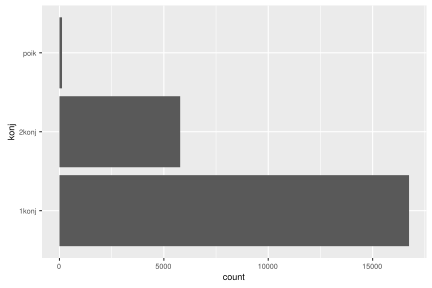
\includegraphics[width=0.9\textwidth,keepaspectratio]{../figure/wikidata.pdf}
\caption{Konjugaatioiden yleisyydet Wikisanakirjassa}
\end{figure}
\FloatBarrier

Kuvio osoittaa, että ensimmäiseen konjugaatioon kuuluvien verbien määrä
on huomattavan suuri verrattuna toisen konjugaation verbeihin: tarkkaan
ottaen 16744 verbiä siinä missä toiseen konjugaatioon voidaan laskea
5782 verbiä ja poikkeuksellisiin 122 verbiä. Tilastot eivät varmasti
poikkeusten osalta ole ehdottoman tarkkoja, mutta yhtä kaikki kokeilu
antaa hyvän vahvistuksen sille, että 1. konjugaation verbit todella ovat
selkeässä enemmistössä.

Koska toinen konjugaatio on huomattavasti harvinaisempi, se on hyvä
paikka aloittaa, kun yrittää miettiä, mistä minkäkin taivutustyypin
tunnistaa. Šeljakin (2006: 125--126) esittää, että infinitiivivartalon
perusteella voidaan päätellä verbi 2. konjugaatioon kuuluvaksi, jos

\begin{enumerate}
\def\labelenumi{\arabic{enumi}.}
\tightlist
\item
  infinitiivivartalo päättyy /и/-äänteeseen \emph{eikä ole osa
  juurimorfia}. Tästä seuraa, että verbit tyyppiä женить, учить,
  звонить, просить ovat toisen konjugaation verbejä, mutta verbit пить,
  шить, бить ensimmäisen, samoin kuin verbit брить (`ajaa (partaa)') ja
  гнить (`pilaantua'). Tämä on ylivoimaisesti suurin ryhmä:
  Wikisanakirjadatan 2. konjugaation sanoista peräti 5086 päättyy
  infinitiivissä \emph{ить}.
\item
  infinitiivivartalo päättyy /а/-vokaaliin, jota edeltää suhuäänne, eikä
  /а/-vokaali säily preesensvartalossa. Tämä tarkoittaa verbejä tyyppiä
  слышать, держать, прозвучать, лежать. Lisäksi a:han ilman suhuäännettä
  päättyvät спать ja гнать. Jos /a/ säilyy preesensvartalossa, kyseessä
  on 1. konjugaation sana (обещать ym.). Wikisanakirjan aineistossa
  tämän ryhmän sanoja on 243.
\item
  infinitiivivartalo päättyy /а/-vokaaliin ja sitä edeltää vokaali
  j-äänne: стоять, бояться. Wikisanakirjadatassa näitä tapauksia on 27
  ja kaikki ovat johdoksia edellä mainituista kahdesta verbistä
  (esimerkiksi простоять, достояться, побояться ym.)
\item
  infinitiivimuoto päättyy -еть, eikä е säily preesensvartalossa.
  Tällaisia sanoja on Wikisanakirja-aineistossa 373, esimerkiksi
  прозвенеть, оглядеть, смотреться, захрапеть ym -- usein kyseessä on
  jokin äänen lähettämiseen liittyvä verbi kuten храпеть, звенеть. Jos е
  säilyy preesensvartalossa, verbi kuuluu 1. konjugaatioon kuten
  esimerkiksi покраснеть.
\end{enumerate}

\section{Infinitiivi- ja preesensvartaloiden suhteista ensimmäisessä
deklinaatiossa}\label{infinitiivi--ja-preesensvartaloiden-suhteista-ensimmuxe4isessuxe4-deklinaatiossa}

Tarkastellaan vielä ensimmäisen deklinaation tärkeimpiä sisäisiä
sanaryhmiä, joita tässä erotellaan seitsemän.

\subsection{1. ryhmä}\label{ryhmuxe4}

Produktiivisin ja ylivoimaisesti suurin ryhmä ovat verbit tyyppiä
\emph{читать}, joissa infinitiivivartalon lopussa on jokin vokaaleista
а, е, и/ы tai у (Шелякин 2006: 127). Yhteistä tälle ryhmälle on, että
preesensvartalo loppuu /j/-äänteeseen: читать - читаj-, покраснеть -
покраснеj, дуть - дуj. Tämän lisäksi infinitiivivartalon viimeinen
vokaali on preesensvartalossa joskus eri: открыть - откроj, мыть - моj,
брить - брej sekä и--j-vaihtelu sanoissa ltyyppiä /бить/--/бью/т
(foneettisesti: /би/т'/--/бj/ут/).

\subsection{2. ryhmä}\label{ryhmuxe4-1}

Toisen 1. konjugaation sisäisen ryhmän muodostavat ne tutut verbit,
joiden infinitiivivartalo päättyy /ова/ (tai /ева/) ja preesensvartalo
/уj/: /интерес/ова/ -- /интерес/уj/, /жева/ -- /жуj/ (жевать, `purra').

\subsection{3. ryhmä}\label{ryhmuxe4-2}

Hieman edellisen kaltainen ryhmä ovat verbit tyyppiä давать. Näillä
infinitiivivartalon loppu on muotoa /ава/ ja preesensvartalo /аj/.
Ryhmään kuuluvat esimerkiksi /признава/ть/ -- /призна/j/, /устава/ть/ --
/устаj/.

\subsection{4. ryhmä}\label{ryhmuxe4-3}

Seuraavaksi ryhmäksi voidaan erottaa verbit tyyppiä \emph{писать}.
Näissä infinitiivivartalo päättyy /а/-vokaaliin, ja preesensvartalo
eroaa infinitiivivartalosta juurimorfin viimeisen konsonantin osalta:
/писа/ -- /пиш/, /плака/ -- /плач/.\footnote{Huomaa, ettei näitä verbejä
  pidä sekoittaa niihin ensimmäisen konjugaation verbeihin, joilla
  tapahtuu preesensvartalon sisällä äänteenmuutos /о/-alkuisissa
  muodoissa (ks. жить edellä).} Šeljakinin (2006: 129) mukaan tämän
tyypin verbejä on noin sata (писать, сказать, двигать,
махать,искать,брызгать ym.).

\subsection{5. ryhmä}\label{ryhmuxe4-4}

Verbit, joiden infinitiivivartalo päättyy \emph{ну}, voidaan jakaa
kahteen ryhmään sen perusteella, miten niiden preteritimuodot
muodostetaan. Ensimmäiseen ryhmään kuuluvat \emph{momentaaniset}
(одноактный) verbit tyyppiä толкнуть, joilla preteritimuoto muodostetaan
suoraan infinitiivivartalon perusteella (/толкну/л/). Toisen ryhmän
muodostavat verbit tyyppiä \emph{остынуть} (`jäähtyä, haaleta'), jotka
ilmaisevat asteittaista olotilan muutosta ja joiden preteritimuodoissa
ну-suffiksi katoaa taivutuspäätteen edeltä (остыл). Näitä jälkimmäisiä
verbejä on selvästi vähemmän, Šeljakinin (2006: 129) mukaan noin
viisikymmentä. Kummassakin tapauksessa preesensvartalo päättyy /н/
(толкн -- остын). Yhteensä näitä ryhmiä edustaa Wikisanakirjan
aineistossa 926 verbiä, esimerkiksi подвинуть, шагнуть, замёрзнуть
(preteriti замёрз).

\subsection{6. ryhmä}\label{ryhmuxe4-5}

Šeljakin (2006: 133) laskee perustellusti omaksi ryhmäkseen verbit
tyyppiä начать/обнять (`halata') / понять/нажать (`painaa'), joissa
preesensvartalo eroaa melko selkeästi infinitiivivartalosta. Muodostus
noudattaa mallia /нача/ -- /начн/, /обня/ -- /обним/, /поня/ -- /пойм/,
/нажа/ -- /нажм/. Kaikissa tapauksissa siis preesensvartaloon ilmestyy
nasaali /м/ tai /н/ sekä tämän lisäksi joko /и/ tai /j/.

\subsection{7. ryhmä}\label{ryhmuxe4-6}

Ehkä haastavimman ryhmän muodostavat verbit, joissa tapahtuu edellä
mainittu äänteenmuutos muissa kuin yksikön ensimmäisessä ja monikon
kolmannessa persoonassa. Lisäksi tämän ryhmän verbeillä esiintyy
esimerkiksi väistyvän vokaalin ilmiötä. Ryhmän muodostavat seuraavat
alaluokat:

\begin{itemize}
\tightlist
\item
  infinitiivissä \emph{-чь} päättyvät verbit tyyppiä печь, жечь, лечь,
  joilla infinitiivi- ja preesensvartalot ovat identtiset. Huomaa
  väistyvä vokaali жечь-verbillä (infinitiivi жечь, mutta preesensmuodot
  /жг/у, /жжёшь/ jne.) лечь-verbillä puolestaan on preesensmuodoissa
  vartalon lopussa a-vokaali: лягу, ляжешь ym.
\item
  infinitiivissä /сти/ tai /зти/ tai /сть/ päättyvät verbit kuten
  нести,спасти, везти, красть ja попасть. Näillä verbeillä äänteenmuutos
  tapahtuu liudentumattomien ja liudentuneiden konsonanttien välillä,
  kuten (selvyyden vuoksi foneettisesti esitettynä) /вез/у -- /вез'/ош
  ja /попад/у -- /попад'/ош/. Osalla сти-infinitiivin saavista verbeistä
  sekä kaikilla сть-infinitiivin saavista preteritin vartalo päättyy
  vokaaliin ja saa peräänsä normaalin л-tunnuksen (vrt. везти -- вёз ja
  брести -- брёл / попасть -- попал).
\item
  Edellisen kaltainen alaryhmänsä ovat verbit плыть ja жить, joilla
  preesensvartalo loppuu infinitiivivartalossa esiintymättömään
  в-konsonanttiin ja on siis muotoa /жив/ tai /плыв/ ja joilla myös
  toteutuu äänteenmuutos liudentuneiden ja liudentumattomien
  konsonanttien välillä. Vastaavasti verbillä учесть preesensvartalossa
  on ``ylimääräinen'' \emph{т}: учесть -- /учт/. Myös verbit tyyppiä
  умереть kuuluvat tähän ryhmään: niilläkin tapahtuu vaihtelu
  liudentuneen ja liudentumattoman konsonantin välillä. Lisäksi
  havaitaan väistyvä vokaali: infinitiivivartalo on muotoa /умере/,
  preesensvartalo /умр/.
\end{itemize}

\section{Epäsäännöllisesti taipuvia
verbejä}\label{epuxe4suxe4uxe4nnuxf6llisesti-taipuvia-verbejuxe4}

Edellä käsiteltiin etenkin ensimmäiseen konjugaatioon liittyviä paikoin
melko monimutkaisiakin eroja infinitiivi- ja preesensvartaloiden välillä
sekä preesensvartalon sisällä tapahtuvia äänteenmuutoksia niin
ensimmäisessä kuin toisessakin konjugaatiossa. Vaikka kuvatut ilmiöt
tekevät venäjän verbitaivutuksesta melko laajan ilmiön, voidaan todeta,
että loppujen lopuksi suuri osa verbeistä sopii kuitenkin joko
ensimmäiseen tai toiseen konjugaatioon -- poikkeuksia ja
sekataivutustapauksia ei ole älyttömän paljon. Wikisanakirjan
aineistossa varsinaisten poikkeustapausten luokkaan osuu vain 122
tapausta (mukana paljon johdoksia) kaikkiaan noin 27 000
verbilekseemistä . Merkittävimpiä näistä lienevät
\href{http://ru.wiktionary.org/wiki/\%D1\%85\%D0\%BE\%D1\%82\%D0\%B5\%D1\%82\%D1\%8C}{хотеть},
\href{http://ru.wiktionary.org/wiki/\%D0\%B1\%D0\%B5\%D0\%B6\%D0\%B0\%D1\%82\%D1\%8C}{бежать},
\href{http://ru.wiktionary.org/wiki/\%D0\%B4\%D0\%B0\%D1\%81\%D1\%82\%D1\%8C}{дасть}
ja
\href{http://ru.wiktionary.org/wiki/\%D0\%B5\%D1\%81\%D1\%82\%D1\%8C}{есть}
(linkit Wikisanakirjaan). Kaksi ensimmäistä sekoittavat 1. ja 2.
deklinaation, дать-verbissä on tyystin omat päätteensä ja
есть-verbilläkin yksikön ensimmäinen persoona saa aivan oman, muista
slaavilaisista kielistä kuten tsekistä tutun m-päätteen sekä eräitä
muutoksia preesensvartaloon.

\section{Muutama sana painoista}\label{muutama-sana-painoista}

Tässä yhteydessä verbien painotyyppeihin ei perehdytä yhtä tarkasti kuin
substantiivien. Šeljakinin (2006: 136) perusteella voidaan kuitenkin
todeta, että verbit jakautuvat painon puolesta kolmeen pääryhmään:

\begin{enumerate}
\def\labelenumi{\arabic{enumi}.}
\tightlist
\item
  Paino aina vartalolla

  \begin{itemize}
  \tightlist
  \item
    Tähän kuuluvat kaikki verbit, joiden infinitiivi päätty painottomaan
    \emph{ать}-tavuun kuten
    \href{http://ru.wiktionary.org/wiki/\%D0\%BE\%D0\%B1Едать}{обЕдать},
    \href{http://ru.wiktionary.org/wiki/\%D0\%BBАять}{лАять},
    \href{http://ru.wiktionary.org/wiki/Ехать}{Ехать} ym. Muutenkin
    edellä esitetty 1. konjugaation ensimmäinen ja suurin alaryhmä
    sisältää käytännössä vain tähän painotyyppiin kuuluvia verbejä
    (poikkeuksena verbit tyyppiä
    \href{http://ru.wiktionary.org/wiki/\%D0\%B1\%D0\%B8\%D1\%82\%D1\%8C}{бить}
    /
    \href{http://ru.wiktionary.org/wiki/\%D0\%BF\%D0\%B5\%D1\%82\%D1\%8C}{петь}).
    Lisäksi suurin osa \emph{ова/ева}-suffiksillisista verbeistä (toinen
    1. konjugaation alaryhmä) kuuluu tähän ryhmään.
  \end{itemize}
\item
  Paino aina päätteellä

  \begin{itemize}
  \tightlist
  \item
    Tähän päätetyyppiin kuuluu suurin osa edellä 1. konjugaation
    seitsemänneksi alaryhmäksi luokitelluista verbeistä
    (\href{http://ru.wiktionary.org/wiki/\%D0\%B6\%D0\%B8\%D1\%82\%D1\%8C}{жить},
    \href{http://ru.wiktionary.org/wiki/\%D0\%BD\%D0\%B5\%D1\%81\%D1\%82\%D0\%B8}{нести},
    \href{http://ru.wiktionary.org/wiki/\%D0\%BA\%D1\%80\%D0\%B0\%D1\%81\%D1\%82\%D1\%8C}{красть}
    ym. MUTTA
    \href{http://ru.wiktionary.org/wiki/\%D0\%BB\%D0\%B5\%D1\%87\%D1\%8C}{лечь},
    \href{http://ru.wiktionary.org/wiki/\%D1\%81\%D0\%B5\%D1\%81\%D1\%82\%D1\%8C}{сесть}).
    Toinen suuri tyhmä ovat toisen konjugaation verbit, joiden
    infinitiivi loppuu painolliseen
    /ить/-tavuun(\href{http://ru.wiktionary.org/wiki/\%D0\%B7\%D0\%B2\%D0\%BE\%D0\%BD\%D0\%B8\%D1\%82\%D1\%8C}{звонить},
    \href{http://ru.wiktionary.org/wiki/\%D1\%82\%D0\%B2\%D0\%BE\%D1\%80\%D0\%B8\%D1\%82\%D1\%8C}{творить}
    ym.). Lisäksi joitakin ова/ева-verbejä
    (\href{http://ru.wiktionary.org/wiki/\%D0\%B6\%D0\%B5\%D0\%B2\%D0\%B0\%D1\%82\%D1\%8C}{жевать},
    \href{http://ru.wiktionary.org/wiki/\%D0\%BE\%D1\%81\%D0\%BD\%D0\%BE\%D0\%B2\%D0\%B0\%D1\%82\%D1\%8C}{основать},
    \href{http://ru.wiktionary.org/wiki/\%D0\%BA\%D0\%BB\%D0\%B5\%D0\%B2\%D0\%B0\%D1\%82\%D1\%8C}{клевать}
    ym.) ja kaikki ава-verbit
    (\href{http://ru.wiktionary.org/wiki/\%D0\%B4\%D0\%B0\%D0\%B2\%D0\%B0\%D1\%82\%D1\%8C}{давать},
    \href{http://ru.wiktionary.org/wiki/\%D0\%BF\%D1\%80\%D0\%B8\%D0\%B7\%D0\%BD\%D0\%B0\%D1\%82\%D1\%8C}{признать}
    ym.).
  \end{itemize}
\item
  Paino aina vartalolla paitsi yksikön ensimmäisessä persoonassa

  \begin{itemize}
  \tightlist
  \item
    Tähän päätetyyppiin kuuluvat kaikki edellä neljänneksi 1.
    konjugaation alaryhmäksi luetellut verbit, jos ne loppuvat
    infinitiivissä painolliseen \emph{ать}-tavuun (писать, махать).
    Lisäksi tähän kuuluu parikymmentä 2. konjugaation painolliseen
    \emph{ить}-tavuun infinitiivissä päättyvä verbiä kuten
    \href{http://ru.wiktionary.org/wiki/\%D0\%B2\%D0\%BE\%D0\%B4\%D0\%B8\%D1\%82\%D1\%8C}{водить},
    \href{http://ru.wiktionary.org/wiki/\%D0\%BA\%D1\%83\%D0\%BF\%D0\%B8\%D1\%82\%D1\%8C}{купить},
    \href{http://ru.wiktionary.org/wiki/\%D0\%BB\%D0\%BE\%D0\%B2\%D0\%B8\%D1\%82\%D1\%8C}{ловить},
    \href{http://ru.wiktionary.org/wiki/\%D0\%BA\%D0\%BE\%D1\%80\%D0\%BC\%D0\%B8\%D1\%82\%D1\%8C}{кормить},
    \href{http://ru.wiktionary.org/wiki/\%D1\%81\%D1\%82\%D1\%83\%D0\%BF\%D0\%B8\%D1\%82\%D1\%8C}{ступить}
    ym.
  \end{itemize}
\end{enumerate}

\section{Partisiippien muodostus}\label{partisiippien-muodostus}

Pohjustetaan nyt tulevaa luentoa pääluokista käymällä läpi vielä yhtä
sananmuodostusoppiin liittyvää teemaa: partisiippien muodostusta.

\subsection{Mitä partisiipit ovat?}\label{mituxe4-partisiipit-ovat}

Verbeillä on niin suomessa kuin venäjässä kahdenlaisia muotoja:
persoonamuotoja (спрягаемые формы глагола) ja nominaali- eli
infiniittimuotoja (неспрягаемые формы глагола). Persoonamuodot taipuvat
suomalaisen nimityksensä mukaisesti persoonissa tai venäjän tapauksessa
menneen ajan muotojen osalta suvussa ja luvussa. Nominaalimuodot
puolestaan muistuttavat taivutukseltaan ja osin myös syntaktiselta
käyttäytymiseltään nomineja, esimerkiksi adjektiiveja. Partisiipit ovat
nominaalimuoto, joita on sekä suomessa että venäjässä mutta jotka eivät
kuitenkaan näissä kahdessa kielessä muodosta identtisiä kategorioita.

Venäjässä partisiipit voidaan jakaa neljään ryhmään riippuen niiden
edustamasta \emph{aikamuodosta} ja \emph{pääluokasta} (molemmat verbien
ilmaisemia kieliopillisia kategorioita).

\begin{enumerate}
\def\labelenumi{\arabic{enumi}.}
\tightlist
\item
  Aktiivin partisiipit

  \begin{itemize}
  \tightlist
  \item
    aktiivin partisiipin preesensmuoto ilmaisee jonkin subjektin jotakin
    ominaisuutta nykyhetkessä: человек, \emph{несущий} ящик. Suomessa
    tätä vastaa niin kutsuttu VA-partisiippi (ks.
    \href{http://scripta.kotus.fi/visk/sisallys.php?p=521}{VISK §521}):
    laatikkoa \emph{kantava} henkilö.
  \item
    aktiivin partisiipin preteritimuotoa puolestaan vastaa suomen
    NUT-partisiippi ja se ilmaisee vastaavaa ominaisuutta menneessä
    ajassa: человек, \emph{нёсший} ящик (laatikkoa \emph{kantanut}
    henkilö)
  \end{itemize}
\item
  Passiivin partisiipit

  \begin{itemize}
  \tightlist
  \item
    passiivin partisiipin preesensmuoto ilmaisee jonkun agentin jollekin
    kohteelle suorittamaa tai suoritettavissa olevaa toimintaa: ящик,
    несомый человеком (ihmisen kantama laatikko). Tätä vastaa usein
    suomen agenttipartisiippi. Toisaalta suomen agenttipartisiippi on
    nimensä mukaisesti sidottu tekijään: asiat ovat aina jonkun
    \emph{tekemiä}, joten kun tekijää ei ilmaista, joudutaan suomessa
    turvautumaan muihin muotoihin. Vertaa esimerkiksi muotoa
    \emph{понимаемый} virkkeessä \emph{Интерес для них представляют
    территории, удовлетворяющие определенным (хотя и не всегда
    однозначно понимаемым) принципам}, jossa partisiippi ilmaistaisiin
    suomeksi pikemminkin `ymmärrettävissä oleva'. Toisaalta lauseessa
    \emph{Деньги должны храниться в хорошо охраняемых помещениях}
    agentittoman passiivin partisiipin preesensmuodon vastineena on
    puhtaasti vain suomen TU-partisiippi (hyvin vartioiduissa).
  \end{itemize}
\end{enumerate}

\subsection{Miten partisiipit
muodostetaan?}\label{miten-partisiipit-muodostetaan}

\subsubsection{Rajoituksia}\label{rajoituksia}

Venäjän partisiipeissa on syytä kiinnittää huomiota siihen, ettei
kaikkia partisiippeja voi muodostaa kaikista verbeistä. Tarkastellaan
ensin, mitä puhtaan sananmuodostuksellisia rajoituksia partisiippien
muodostamiseen liittyy.

\subparagraph{Sananmuodostukselliset
rajoitukset}\label{sananmuodostukselliset-rajoitukset}

Pääpiirteissään sananmuodostuksen tasolla ovat voimassa seuraavat
rajoitukset:

\begin{enumerate}
\def\labelenumi{\arabic{enumi}.}
\tightlist
\item
  Niin aktiivin kuin passiivin partisiipin \textbf{preesensmuotoja}
  muodostetaan vain imperfektiivisen aspektin verbeistä.
\item
  \textbf{Passiivin partisiipin preteritimuotoja} muodostetaan vain
  perfektiivisen aspektin verbeistä.
\item
  \textbf{Aktiivin partisiipin preteritimuotoja} voidaan muodostaa
  aspektista riippumatta.
\end{enumerate}

\subparagraph{Käyttöön liittyvät
rajoitukset}\label{kuxe4yttuxf6uxf6n-liittyvuxe4t-rajoitukset}

Vaikka jokin partisiippimuoto voitaisiin teoriassa muodostaa, on usein
käytännössä niin, ettei muotoa kuitenkaan ole olemassa. Ensinnäkin
partisiippien käyttöä rajoittaa se syntaktinen seikka, että passiivin
partisiippimuotoja muodostetaan pääasiassa transitiiviverbeistä eli
verbeistä, jotka saavat täydennyksekseen suoran objektin (poikkeuksena
esimerkiksi руководить чем, josta voidaan muodostaa passiivin
partisiipin preesensmuoto). Šeljakin (2006: 177) huomauttaa lisäksi
erityisesti passiivin partisiipin preesensmuodoista, että ne ovat
tyyliltään kirjallisia, mistä johtuen monista arkipäiväisistä verbeistä
niitä ei todellisuudessa muodosteta: esimerkiksi verbeistä ругать,
кормить, крыть. Wade (2010: 369) antaa tarkemman luettelon siitä, minkä
tyyppisistä verbeistä ei passiivin partisiipin preesensiä muodosteta.
Waden huomiot ovat pääpiirteissään seuraavia:

\begin{itemize}
\tightlist
\item
  Passiivin partisiipin preesensiä ei muodosteta verbeistä, joiden
  infinitiivi päättyy -чь, -уть, -ереть, -зть, -сть
\item
  Ei myöskään monista yksitavuisista verbeistä kuten бить, брать, мыть,
  шить
\item
  Ei useimmista edellä 1. konjugaation 4. alaryhmäksi nimitetyistä
  verbeistä (писать, плакать, прятать)
\item
  Monet 2. konjugaation verbit ovat sellaisia, ettei niistä muodosteta
  passiivin partisiipin preesensiä. Wade mainitsee esimerkkeinä mm.
  verbit благодарить, платить, портить ja чистить.
\end{itemize}

\subsubsection{Vartalot}\label{vartalot}

Partisiipit muodostetaan venäjässä suffiksien avulla. Nikunlassin (2002:
163) mukaan muodostus voidaan (hieman yksinkertaistaen) tiivistää
toteamalla, että preesensmuotojen pohjana on preesensvartalo,
preteritimuotojen pohjana infinitiivivartalo. Näin ollen edellä
esimerkkinä toimineesta нести-verbistä voidaan preesensmuotojen osalta
todeta:

\begin{enumerate}
\def\labelenumi{\alph{enumi})}
\tightlist
\item
  Aktiivin partisiipin preesens:

  \begin{enumerate}
  \def\labelenumii{\arabic{enumii}.}
  \tightlist
  \item
    Preesensvartalo muodostetaan нести -- /нес/ут/ -- /нес/
  \item
    Aktiivin partisiipin preesens muodostetaan /ущ/-suffiksilla
  \item
    Aktiivin partisiipin preesensmuodon vartaloksi saadan /нес/ущ/
  \item
    Partisiippimuotojen taivutuspäätteet ovat adjektiivideklinaation
    mukaiset, joten aktiivin partisiipin preesensmuotoja нести-sanasta
    ovat /нес/у/щий/, /нес/ущ/ая/ ym.
  \end{enumerate}
\item
  Passiivin partisiipin preesens:

  \begin{enumerate}
  \def\labelenumii{\arabic{enumii}.}
  \tightlist
  \item
    Preesensvartalo muodostetaan нести -- /нес/ут/ -- /нес/
  \item
    Aktiivin partisiipin preesens muodostetaan /ом/-suffiksilla
  \item
    Aktiivin partisiipin preesensmuodon vartaloksi saadan /нес/ом/
  \item
    Partisiippimuotojen taivutuspäätteet ovat adjektiivideklinaation
    mukaiset, joten aktiivin partisiipin preesensmuotoja нести-sanasta
    ovat /нес/ом/ый/, /нес/ом/ая/ ym.
  \end{enumerate}
\end{enumerate}

Preteritimuotojen kohdalla on parempi käyttää esimerkkinä jotakin
säännöllisen infinitiivivartalon verbiä, esimerkiksi прочитать:

\begin{enumerate}
\def\labelenumi{\alph{enumi})}
\tightlist
\item
  Aktiivin partisiipin preteriti:

  \begin{enumerate}
  \def\labelenumii{\arabic{enumii}.}
  \tightlist
  \item
    Infinitiivivartalo muodostetaan /прочита/ть -- /прочита/
  \item
    Aktiivin partisiipin preteriti muodostetaan /вш/-suffiksilla
  \item
    Aktiivin partisiipin preteritimuodon vartaloksi saadaan /прочита/вш/
  \item
    Partisiippimuotojen taivutuspäätteet ovat adjektiivideklinaation
    mukaiset, joten aktiivin partisiipin preesensmuotoja
    прочитать-sanasta ovat /прочита/вш/ий, /прочита/вш/ая ym.
  \end{enumerate}
\item
  Passiivin partisiipin preteriti:

  \begin{enumerate}
  \def\labelenumii{\arabic{enumii}.}
  \tightlist
  \item
    Infinitiivivartalo muodostetaan /прочита/ть -- /прочита/
  \item
    Passiivin partisiipin preteriti muodostetaan /нн/-suffiksilla
  \item
    Aktiivin partisiipin preteritimuodon vartaloksi saadaan /прочита/нн/
  \item
    Partisiippimuotojen taivutuspäätteet ovat adjektiivideklinaation
    mukaiset, joten aktiivin partisiipin preesensmuotoja
    прочитать-sanasta ovat /прочита/нн/ый, /прочита/нн/ая ym. Lisäksi
    voidaan muodostaa lyhyet muodot /прочита/н/ø/,/прочита/н/а/ ym.,
    joissa /онн/-suffiksin sijasta on suffiksi /он/
  \end{enumerate}
\end{enumerate}

\subsubsection{Suffiksit}\label{suffiksit}

Partisiippien muodostamisessa käytettävät suffiksit vaihtelevat jonkin
verran. Seuraavassa käydään läpi vaihtelut muodostussuffikseissa
partisiipeittain (tarkemmin ks. Nikunlassi 2002: 162, Шелякин (2006):
175--178).

\subparagraph{Preesenspartisiipit}\label{preesenspartisiipit}

Partisiippien preesensmuotojen muodostus on selkeää. Aktiivin
partisiipin preesensin suffikseja on kaksi: /ущ/ ja /ащ/. Nämä
jakautuvat siististi niin, että 1. konjugaation verbeillä suffiksi on
/ущ/, 2. konjugaation verbeillä /ащ/. Passiivin partisiipin
preesensmuodoissa 1. konjugaation suffiksi on /ом/ ja 2. konjugaation
suffiksi /им/. Huomaa jälleen kerran, että /ом/-suffiksin vokaali on
painollisen tavun jälkeinen redusoitunut /о/, jota liudentuneen
konsonantin tai j-äänteen jäljessä merkitään е-kirjaimella.

Tarkastellaan esimerkkiä kummastakin konjugaatiosta.

\begin{enumerate}
\def\labelenumi{\alph{enumi})}
\tightlist
\item
  Verbi /покупать/ kuuluu 1. konjugaatioon. Preesenspartisiipit
  muodostetaan preesensvartalosta, joka tässä tapauksessa on /покупаj/.

  \begin{itemize}
  \tightlist
  \item
    Aktiivin partisiipin tunnus 1. konjugaatiolla on /ущ/, joten
    muodoksi saadaan: /покупаj/ущ/ий/.
  \item
    Passiivin partisiipin tunnus 1. konjugaatiolla on /ом/ joten
    muodoksi saadaan /покупа/ем/ый (foneettisessa asussaan
    /покупаj/ом/ый)
  \end{itemize}
\item
  Verbi /держать/ kuuluu 2. konjugaatioon. Preesenspartisiipit
  muodostetaan preesensvartalosta, joka tässä tapauksessa on /держ/.

  \begin{itemize}
  \tightlist
  \item
    Aktiivin partisiipin tunnus 2. konjugaatiolla on /ащ/, joten
    muodoksi saadaan: /держ/ащ/ий/.
  \item
    Passiivin partisiipin tunnus 1. konjugaatiolla on /им/ joten
    muodoksi saadaan /держ/им/ый
  \end{itemize}
\end{enumerate}

Kuten todettu, preesenspartisiipit muodostetaan säännönmukaisesti
preesensvartalosta. Poikkeuksen muodostavat kuitenkin edellä 1.
konjugaation toiseksi alaryhmäksi nimetty joukko, jonka verbeillä
\emph{passiivin partisiipin} muodostus tapahtuu infinitiivivartalon
perusteella. Esimerkiksi sanat признавать ja давать saavat siis
muodoiksi признаваемый/даваемый (eivätkä preesensvartaloon pohjautuvia
*признаюемый/*даюемый).

\subparagraph{Aktiivin partisiipin
preteriti}\label{aktiivin-partisiipin-preteriti}

Aktiivin partisiipin preteritissä on myös kaksi eri vaihtoehtoa
suffiksille: /вш/ tai /ш/. Ensimmäistä käytetään, jos verbin
infinitiivivartalo päättyy vokaaliin, toista muissa tapauksissa.
Selkeitä sanoja tässä suhteessa ovat sanat, joilla infinitiivin tunnus
on tavallinen \emph{ть}: /прочита/вш/ий/, /игра/вш/ий,
/рассматрива/вш/ий jne. Enemmän pohdiskelua vaativat чь-, сть ja
сти-infinitiivit.

Pohditaan ensin чь-päätteisiä verbejä, esimerkiksi verbejä печь ja
стричь (`leikata hiuksia'). Edellä todettiin, että infinitiivivartalo on
näillä verbeillä preesensvartalon kaltainen eli muodostetaan /печь/ --
/пек/ут/ -- /пек/ ja /стричь/ -- /стриг/ут/ -- /стриг/. Näissä
tapauksissa infinitiivivartaloita ovat siis пек ja стриг, jotka
päättyvät konsonanttiin. Partisiipin muodostava suffiksi on siis /ш/,
joten aktiivin partisiipin preteritimuodot ovat /пёк/ш/ий/ ja
/стриг/ш/ий/ (huomaa kuitenkin painollinen о-vokaali пёкший-sanassa).

Myös сти-verbeistä todettiin edellä, että infinitiivivartalo on
preesensvartalon kaltainen. Näin ollen нести-verbin infinitiivivartalo
on /нести/ -- /нес/ут/ -- /нес/. Koska vartalo päättyy konsonanttiin,
käytetään /ш/-suffiksia ja aktiivin partisiipin preteritimuodoksi
saadaan /нёс/ш/ий (tässäkin tapauksessa vartalon vokaalina o).
Esimerkiksi Повести-verbistä infinitiivivartalo taas on /повед/, joten
aktiivin partisiipin preteritissä saadaan /повед/ш/ий. Erikseen on
mainittava идти-verbi, jonka partisiippimuodossa vartalo muuttuu
kokonaan ja on /шед/ш/ий.

Чь- ja сти-päätteisten verbien tavoin myös сть-päätteisillä verbeillä
infinitiivivartalo on preesensvartalon kaltainen: /сес/ть/ -- /сяд/,
/упас/ть/ -- /упад/. Näillä verbeillä partisiipin muodostus ei
kuitenkaan noudata edellä kuvattua logiikkaa, vaan verbit saavat
вш-suffiksin, joka liitetään preteritimuodon vartaloon. Aktiivin
partisiipin preteritimuodot ovat tällöin: сесть -- /се/вш/ий/ ja упасть
-- /упа/вш/ий/.

\subparagraph{Passiivin partisiipin
preteriti}\label{passiivin-partisiipin-preteriti}

Passiivin partisiipin preteritin muodostamiseksi on muita partisiippeja
enemmän eri suffikseja. Vaihtoehtoja ovat /нн/, /онн/ ja /т/. Muodostus
on edellisiä partisiippeja hankalampaa myös siinä mielessä, että siihen
liittyy äänteenmuutoksia. Suffiksit jakautuvat seuraavasti:

\begin{enumerate}
\def\labelenumi{\arabic{enumi}.}
\tightlist
\item
  Jos verbin infinitiivivartalo päättyy а-suffiksiin, on partisiipin
  muodostava suffiksi muotoa /нн/. Esimerkiksi прочитать-verbillä
  infinitiivivartalo muodostetaan /прочитать/ -- /прочита/ть/ ja se
  loppuu /а/-suffiksiin. Partisiippimuoto on siis /прочита/нн/ый/.
\item
  Hankaluutena edellisen kohdan osalta on, että verbien
  infinitiivivartalon vokaali voi olla /а/, vaikka kyseessä ei olisikaan
  verbinmuodostussuffiksi -- /а/ voi nimittäin olla osa verbin
  juurimorfeemia, kuten sanoissa /нача/ть. Tällaisia ovat itse asiassa
  kaikki edellä 1. konjugaation 6. ryhmäksi luetellut verbit: нажать,
  понять, принять jne. Näissä tapauksissa partisiippi muodostetaan
  /т/-suffiksilla: /нажа/т/ый, /нача/т/ый jne. lukuun ottamatta eräitä
  poikkeuksia: дать -- данный.
\item
  /т/-suffiksia puolestaan käytetään myös, jos infinitiivivartalo
  päättyy /ну/, /ере/ tai -/о/. Esimerkiksi /вытереть/-verbin
  infinitiifivartalo on /вытере/. Tästä muodostetaan passiivin
  partisiipin preteriti poistamalla viimeinen vokaali ja lisäämällä
  /т/-suffiksi: /вытер/т/ый. /Затянуть/-verbin vartalo on puolestaan
  /затяну/ ja partisiippimuoto /затЯнутый/.
\item
  Jos verbin infinitiivivartalo päättyy konsonanttiin, partisiippi
  muodostetaan suffiksilla /онн/. Esimerkiksi провести-verbillä
  preesens- ja infinitiivivartalo ovat yhtenevät, joten
  infinitiivivartalokin muodostetaan /провед/ут -- /провед/. Tähän
  liitetään /онн/-suffiksi, jolloin partisiippimuodoksi saadaan
  /провед/ённ/ый. Lisäksi tämän päätteen saavat toisen konjugaation
  verbit, joiden infinitiivivartalo päättyy /и/- tai /е/-suffiksiin.
  Tällaisia ovat esimerkiksi исказить (`vääristää') ja просмотреть.
  Исказить-verbin infinitiivivartalo on /искази/. Partisiippia
  muodostaessa /и/-suffiksi häviää ja tilalle liitetään /онн/-suffiksi:
  /искаж/ённ/ый/. Kuten huomaat, samalla tapahtuu äänteenmuutos.
  Онн-suffiksin edellä tapahtuvat äänteenmuutokset ovat itse asiassa
  samoja kuin 1. ja 2. konjugaatioiden persoonapäätteiden kohdalla
  havaittiin. Просмотреть-verbissä puolestaan
  /просмотре/-infinitiivivartalosta häviää /е/-suffiksi ja se korvautuu
  /онн/-suffiksilla: /просмОтр/енн/ый/. Huomaa jälleen kerran, että
  liudentuneen konsonantin jäljessä painoton /о/-äänne kirjoitetaan
  е:nä.
\end{enumerate}

\chapter{Pääluokka kieliopillisena
kategoriana}\label{luento-14-puxe4uxe4luokka-kieliopillisena-kategoriana}


\emph{Pääluokka} (залог) on kieliopillinen kategoria, joka on yksinomaan
verbien ominaisuus. Kategorialla on kaksi arvoa: aktiivi (действительный
залог) ja passiivi (страдательный залог).

Pääluokkakategorian oletusarvona voi hyvin pitää aktiivia: verbit ovat
\emph{useimmiten} aktiivissa, ja passiivinen käyttö on niin suomessa
kuin venäjässäkin aina jonkinasteinen poikkeus. Tässä yhteydessä onkin
kysyttävä funktionaalisen morfologian kannalta tärkeä kysymys: Milloin
ja mihin passiivia tarvitaan?

Marjatta Vanhala-Aniszewskin (1992: 242) mukaan passiivin tärkein
funktio niin suomessa kuin venäjässä on huomion vieminen pois toiminnan
varsinaisesta suorittajasta (дефокусировка реального производителя
действия). Vertaa tähän liittyen seuraavia lauseita:

\begin{enumerate}
\def\labelenumi{(\arabic{enumi})}
\setcounter{enumi}{221}
\tightlist
\item
  Я написал книгу как для современников, так и для потомков
\item
  Книга написана как для современников, так и для потомков
\end{enumerate}

Yksinkertaisimmillaan aktiivin ja passiivin erossa on kyse lauseiden 222
ja 223 välisestä erosta: lauseessa 222 on selvästi ilmaistu, kuka on
vastuussa suoritetusta toiminnasta, kun taas lause 223 jättää tämän
auki. Monimutkaisemmaksi ero muuttuu, kun ajatellaan passiivilauseita,
joissa tekijä ilmaistaan agenttitäydennyksen avulla:

\begin{enumerate}
\def\labelenumi{(\arabic{enumi})}
\setcounter{enumi}{223}
\tightlist
\item
  Книга написана Достоекским.
\end{enumerate}

Kuitenkin myös lauseesta 224 voidaan todeta, ettei päähuomio ole
tekijässä vaan tekemisen kohteessa: tekijän ilmaiseminen on ainoataan
täydentävää informaatiota.

\section{Passiivirakenteet
venäjässä}\label{passiivirakenteet-venuxe4juxe4ssuxe4}

Venäjästä erotetaan tavallisesti kaksi erityyppistä passiivirakennetta
ja näiden lisäksi kolmas rakenne, jota käytetään passiivin funktiossa.
Varsinaisia (morfologisessa ja syntaktisessa mielessä)
passiivirakenteita ovat \emph{morfologinen} (ся-passiivi) ja
\emph{perifrastinen} passiivi (морфологический / перифрастический
пассив) (Vanhala-Aniszewski 1992: 60). Kaikkiin passiivirakenteisiin
liittyy olennaisena vaatimuksena verbin transitiivisuus: toisin sanoen
intransitiiviverbejä kuten бежать, расти, работать ei voi käyttää
passiivissa.

\subsection{Morfologinen passiivi}\label{morfologinen-passiivi}

Morfologinen passiivi muodostetaan nimensä mukaisesti morfologisin
keinoin, lisäämällä postfiksi /ся/ \emph{imperfektiivistä aspektia
edustavaan} verbiin. Koska se muodostetaan imperfektiivisen aspektin
verbeistä, seurauksena on, että morfologisella passiivilla kuvattava
toiminta on aina \emph{prosessuaalista} (процессный), se ei koskaan
saavuta suoritetun toiminnan rajaa tai voi kertoa loppuun saatetusta
prosessista. Morfologinen passiivi voidaan muodostaa niin menneen
(esimerkit 228, 229) kuin ei-menneen ajan muodoista (esimerkit 225, 226,
227), mukaan lukien futuurimuodot.

\begin{enumerate}
\def\labelenumi{(\arabic{enumi})}
\setcounter{enumi}{224}
\tightlist
\item
  Завод \emph{строится} на новой промышленной площадке
\item
  Тема \emph{будет обсуждаться} и на проводимой Высшей школой экономики
  Четвёртой ежегодной конференции
\item
  Узбекский хлеб \emph{печётся} в традиционных глиняных печах --
  тандырах.
\item
  Все детали будущего дома \emph{изготавливались} для вас на
  домостроительных комбинатах
\item
  Выяснилось, самолет \emph{проектировался} еще в начале пятидесятых
  специалистами фирмы «Локхид эркрафт корпорейшен»
\end{enumerate}

\subsection{Perifrastinen passiivi}\label{perifrastinen-passiivi}

Perifrastisella passiivilla tarkoitetaan partisiippien ja быть-verbin
avulla muodostettavaa passiivirakennetta. Tarkkaan ottaen rakenne
muodostetaan passiivin partisiipin preteritin lyhyistä muodoista. Kuten
edelliseltä luennolta muistat, passiivin partisiipin preteritimuotoja
tehdään \emph{ainoastaan perfektiivisen aspektin verbeistä}, joten
perifrastinen passiivi heijastelee perfektiivisen aspektin ominaisuuksia
siinä missä morfologinen passiivi imperfektiivisen aspektin. Myös tätä
passiivimuotoa on mahdollista käyttää niin menneen (esimerkit 230, 231)
kuin ei-menneen ajan toiminnasta (esimerkki 232).

\begin{enumerate}
\def\labelenumi{(\arabic{enumi})}
\setcounter{enumi}{229}
\tightlist
\item
  Данная технология \emph{была использована} для подготовки входных
  тестов по математике
\item
  Вертолёт \emph{был обнаружен} 6 сентября в Ингушетии
\item
  Особое внимание \emph{будет уделено} наращиванию международного
  партнерского сотрудничества
\end{enumerate}

Perifrastista passiivia voidaan käyttää myös ilman быть-verbiä. Tällöin
on Vanhala-Aniszewskin (1992: 66) mukaan kyse niin kutsutusta passiivin
perfektimerkityksestä (перфект пассива). Keskeisintä tässä merkityksessä
on ajatus siitä, että toiminnan tulos on puhehetkellä voimassa. Näin
ollen esimerkissä 233 Hodorkovski on puhehetkellä pidätettynä (merkitys
on staattinen), kun taas быть-verbin sisältävässä esimerkissä 234
pidätys kuvataan menneisyydessä tapahtuneena toimintana, jonka tuloksen
ei oleteta olevan enää voimassa:

\begin{enumerate}
\def\labelenumi{(\arabic{enumi})}
\setcounter{enumi}{232}
\tightlist
\item
  Ходорковский арестован
\item
  Ходорковский был арестован (после чего его повезли в Москву для
  допросов)
\end{enumerate}

\subsection{Indefiniittis-persoonainen
rakenne}\label{indefiniittis-persoonainen-rakenne}

Indefiniittis-persoonaiset (неопределенно-личные) rakenteet eivät ole
morfologian tai syntaksin kannalta varsinaisia passiivimuotoja, mutta
niitä yhtä kaikki käytetään samaan tarkoitukseen kuin passiivia: ennen
kaikkea varsinaisen tekijän häivyttämiseen tai identifioimatta
jättämiseen. Kiinnostavaa kyllä, juuri indefiniittis-persoonaiset
rakenteet vastaavat esimerkiksi Nikunlassin (2002: 162, 203) mukaan
kaikkein lähimmin suomen passiivirakenteita.

Indefiniittis-persoonaiset rakenteet muodostetaan venäjässä
tavallisimmin jättämällä lauseesta pois subjekti ja käyttämällä verbin
monikon kolmannen persoonan muotoa tai monikon preteritimuotoa. Lisäksi
on mahdollista käyttää быть-verbiä ja lyhyttä adjektiivia tai passiivin
partisiipin preteritin lyhyttä neutrimuotoa, jota usein (muttei aina)
seuraa infinitiivi. Šeljakin (2006: 261) antaa kustakin
indefiniittis-persoonaisesta lausetyypistä seuraavat esimerkit.
Esimerkissä 235 muodostuksen pohjana on monikon kolmas persoona,
esimerkissä 236 preteritin monikkomuoto, esimerkissä 237
partisiippimuoto infinitiivin kanssa ja esimerkissä 238 partisiippimuoto
ilman infinitiiviä.

\begin{enumerate}
\def\labelenumi{(\arabic{enumi})}
\setcounter{enumi}{234}
\tightlist
\item
  По радио передают последние известия
\item
  Выставку открыли вчера
\item
  В школе были довольны его работой
\item
  Нам рекомендовано отменить поход в горы
\item
  В городе построено много домов
\end{enumerate}

Tässä yhteydessä on hyvä mainita, että indefiniittis-persoonaista
rakennetta muistuttavat myös \emph{geneeris-persoonaiset}
(обобщенно-личные) rakenteet. En tarkastele niitä kuitenkaan yhtenä
passiivin ilmaisun keinona, vaan kyseessä on ennemminkin, nimensä
mukaisesti, pyrkimys yleistää jokin ilmiö yhden esimerkkitapauksen
perusteella tarkoittamaan ketä tahansa ihmistä tai jonkin konkreettisen
ryhmän (lapset, opiskelijat ym.) edustajaa. Tässä merkityksessä
tavallinen on etenkin yksikön toinen persoona: \emph{если ты знаешь
иностранные языки, найти работу будет нетрудно}.

\subsection{Passiivilauseen agentti}\label{passiivilauseen-agentti}

Toisin kuin suomessa, venäjässä passiivilauseenkin tekijä voidaan
erikseen mainita. Tähän käytetään niin kutsuttua
\emph{agenttitäydennystä} (агентивное дополнение), joka ilmaistaan
instrumentaalilla. Esimerkiksi virkkeeseen 234 voitaisiin liittää
tekijä, jolloin saataisiin virke 240. Tekijä voidaan lisätä myös
morfologisesti muodostettuun passiivirakenteeseen, jolloin esimerkistä
225 saadaan 241:

\begin{enumerate}
\def\labelenumi{(\arabic{enumi})}
\setcounter{enumi}{239}
\tightlist
\item
  Ходорковский был арестован полицией
\item
  Завод строится компанией ``NCC''.
\end{enumerate}

Huomaa kuitenkin, että vaikka tekijän ilmaisu on mahdollista, se ei ole
yleistä. Vanhala-Aniszewskin (1992: 244--245) mukaan agenttimuotoja
käytetään lähinnä virallisessa asiatyylissä ja tieteellisessä tyylissä.
Nikunlassi (2002: 200) puolestaan esittää jopa tarkan luvun: vain
20\%:ssa passiivimuodoista on ilmaistu agentti.

\chapter{Aika ja aspekti kieliopillisina
kategorioina}\label{luento-15-aika-ja-aspekti-kieliopillisina-kategorioina}


Aika on varsin poikkitieteellinen käsite. Se on merkittävä niin
filosofisessa, psykologisessa, lingvistisessä kuin fysikaalisessakin
mielessä. On luonnollista, että ajan ilmaiseminen kielessä on yksi
keskeisimmistä ja tärkeimmistä kysymyksistä, joita niin kielenoppija
kuin -tutkija joutuu pohtimaan. Menemättä sen syvempiin filosofisiin
pohdintoihin, todettakoon käytännön tasolla, että ajan ja ajallisten
suhteiden ilmaisuun voidaan luonnollisissa kielissä käyttää ainakin
\emph{verbien aikamuotoja}, \emph{aspektia}, \emph{adverbeja} sekä
esimerkiksi kiinan kielessä olevia \emph{temporaalipartikkeleita} (Klein
{[}1994{]} 1999, 143). Tällä ja seuraavilla kahdella luennollolla
keskitymme kahteen ensiksi mainittuun kieliopilliseen kategoriaan:
aikamuotoihin eli tempukseen (категория времени) sekä aspektiin
(категория вида).

\section{Aikamuodot venäjässä}\label{aikamuodot-venuxe4juxe4ssuxe4}

Aikaa ja aspektuaalisuutta paljon tutkineen kielitieteilijän A.V.
Bondarkon (2005: 261) mukaan venäjässä käytössä olevat aikamuodot
(aikakategorian arvot) on perinteisimmän tulkinnan mukaisesti jaettu
seuraavan taulukon kuvaamalla tavalla:

\begin{longtable}[c]{@{}lll@{}}
\toprule
Aika & muoto1 & muoto 2\tabularnewline
\midrule
\endhead
Mennyt (preteriti) & прошедшее несовершенное & прошедшее
совершенное\tabularnewline
Nykyhetki (preesens) & настоящее несовершенное & -\tabularnewline
Tuleva (futuuri) & будущее несовершенное & будущее
совершенное\tabularnewline
\bottomrule
\end{longtable}

Taulukko kiinnittää huomion siihen, että aikaa ilmaistaessa
aikamuotokategoria ja aspektikategoria toimivat venäjässä yhteistyössä:
ei oikeastaan ole mahdollista puhua aikamuodoista puhumatta myös
aspektista. On tähdennettävä, että esitetyt muodot koskevat ainoastaan
\emph{indikatiivin} tapaluokkaa (изъявительное наклонение). Tutkitaan
vielä toista versiota taulukosta, jossa käsitteiden nimet on korvattu
konkreettisilla esimerkeillä, verbien открыть ja открывать
indikatiivimuodoilla:

\begin{longtable}[c]{@{}lll@{}}
\toprule
Aika & muoto1 & muoto 2\tabularnewline
\midrule
\endhead
Mennyt (preteriti) & открывал & открыл\tabularnewline
Nykyhetki (preesens) & открываю & -\tabularnewline
Tuleva (futuuri) & буду открывать & открою\tabularnewline
\bottomrule
\end{longtable}

Kummassakin esitetyistä taulukoista on silmiinpistävää, että yksi solu
on tyhjänä. Menneestä ja tulevasta ajasta on esitetty aspektien
(perfektiivinen aspekti, совершенный вид; imperfektiivinen aspekti,
несовершенный вид) mukaiset muodot: прошедшее несовершенное/совершенное
(imperfektiivinen/perfektiivinen preteriti), будущее
несовершенное/совершенное (imperfektiivinen/perfektiivinen futuuri).
Nykyhetkestä ei ole kuitenkaan erotettu muotoa ``настоящее совершенное''
(perfektiivinen preesens). Pohditaan tätä hieman tarkemmin.

Yksi perfektiivisen aspektin tärkeimmistä ominaisuuksista on, että se
ilmaisee toiminnan yhtenä ehjänä kokonaisuutena: se on ikään kuin
molemmista päistään rajattu jana, jota ei voi paloitella pienempiin
osiin:

\textbar{}---------------\textbar{}

Tehdään tähän liittyen ajatusleikki. Kuvittele \emph{avaamista}
toimintana. Ajattele vaikka itsesi avaamassa kirjaa:

\begin{figure}[htbp]
\centering
\includegraphics{../figure/openbook.jpeg}
\caption{}
\end{figure}

Ajattele edelleen, että sillä hetkellä, kun kätesi on jo ottanut kirjan
etukannesta kiinni ja nostanut sitä muutaman sentin, joku kysyy sinulta,
mitä teet. Vastaat tietenkin ``Avaan kirjaa.'' (huomaa suomen objektin
partitiivi). Jos kirjan avaaminen kuvattaisiin nyt edellisen kaltaisella
janalla\ldots{}

Avaaminen alkaa \textbar{}---------------\textbar{} Avaaminen päättyy

\ldots{}olisi sinut puhehetkellä (H) sijoitettava janalle jotakuinkin
seuraavalla tavalla:

Avaaminen alkaa \textbar{}----H---------\textbar{} Avaaminen päättyy

Mitä kaikki tämä kertoo tekemästäsi kirjan avaamisesta toimintana? Sen,
\emph{ettei toimintaa esitetä yhtenä ehjänä, suljettuna kokonaisuutena}
(целостное действие). Voisi sanoa, että sinä puhujana ikään kuin ``astut
toiminnan keskelle'', sen sisään. Venäjässä tällainen sisälle astuminen
on mahdollista imperfektiivisen aspektin verbeillä, \emph{muttei
perfektiivisen aspektin verbeillä}. Nikunlassin (2002: 176) mukaan juuri
tästä seuraa, että perfektiivisen aspektin verbit eivät voi samalla
tavoin ilmasta nykyhetkeä kuin imperfektiivisen aspektin verbit. Mieti
edellistä ajatusleikkiä ja siinä annettua vastausta venäjäksi.
Kysymykseen ``Что ты делаешь?'' on mahdollista vastata ainoastaan
``Открываю книгу''. Jos vastaus olisi ``Открою книгу'', sijoittuisi
toiminta tulevaan siitä syystä, että perfektiivinen aspekti ei annan
mahdollisuutta hypätä keskelle verbin kuvaamaa toimintaa vaan pakottaa
kuulijan kuvittelemaan toiminnan yhtenä kokonaisuutena.

\section{Aikamuotojen
muodostaminen}\label{aikamuotojen-muodostaminen}

Siirrytään nyt tarkastelemaan venäjän aikamuotoja sananmuodostusopin
kannalta. Preesensin muodostaminen oikeastaan kävi ilmi jo edellisestä:
se tehdään imperfektiivisen aspektin verbeistä taivuttamalla niitä
persoonamuodoissa\footnote{Tässä esittämäni kuvaus on tarkoituksellisen
  yksinkertaistettu. Todellisuudessa (ks. esim. Bondarko 2005: 262--265)
  myös perfektiivisen aspektin muodot pystyvät ilmaisemaan merkityksiä,
  jotka on tulkittavissa preesensmerkityksiksi.}. Enemmän huomiota on
sen sijaan kiinnitettävä menneen ajan muotoihin.

\subsection{Preteriti}\label{preteriti}

Jos palautetaan mieleen edellä esitetty verbivartaloiden jakaminen
preesens- ja infinitiivivartaloihin, on perussääntö preteritin
muodostamiseen yksinkertainen: verbin \emph{infinitiivivartaloon}
lisätään taivutuspääte /л/. Lisäksi preteriti ilmaisee venäjässä sukua
ja lukua, joten /л/-päätteen perään lisätään vielä lyhyistä
adjektiiveista tutut /ø/ (maskuliinin nollapääte), /а/, /о/ tai /и/.
Monikkoa ilmaisevan /и/-päätteen edellä preteritin tunnus muuttuu
liudentuneeksi: /л'/. Esimerkiksi verbistä открывать saadaan
infinitiivivartalo /открыва/, johon liitetään preteritin pääte:
/открыва/л/. Verbillä /открыть/ infinitiivivartalo on /откры/, joten
preteritimuoto ennen suku-/lukupäätteitä on /откры/л/.

On olemassa joukko tapauksia, joissa preteritin /л/-päätettä ei ilmaista
maskuliinimuodoissa ja joihin liittyy myös muutoksia
inifinitiivivartalossa. Nikunlassi (2002: 157) luettelee tähän liittyen
seuraavat ryhmät:

\begin{enumerate}
\def\labelenumi{\arabic{enumi}.}
\tightlist
\item
  Jos infinitiivivartalo päättyy \emph{ере}, kuten verbeillä
  \emph{умереть} ja \emph{вытереть}. Näillä verbeillä \emph{ере} putuoaa
  pois menneen ajan muodoissa, niin että verbillä вытереть (`pyyhkiä')
  preteritimuodot ovat /вытер/ø, /вытер/л/а, /вытер/л/о ja /вытер/л/и.
  Jos ollaan aivan tarkkoja, maskuliinimuodossa on kaksi nollapäättettä,
  sillä sekä preteriti että suku on ilmaistu nollapäätteellä:
  /вытер/ø/ø/
\item
  Jos verbi kuuluu edellä ensimmäisen konjugaation viidenneksi
  alaryhmäksi määriteltyyn verbien joukkoon eikä ole momentaaninen verbi
  (kuten толкнуть, махнуть) vaan ilmaisee olotilan muutosta kuten
  \emph{погИбнуть} tai \emph{ослАбнуть}. Tällöin \emph{ну} putoaa pois
  vartalosta kaikissa preteritimuodoissa: /ослаб/ø/ø/, /ослаб/л/а/,
  /ослаб/л/о/, /ослаб/л/и/.
\item
  Jos verbin infinitiivivartalo on sama kuin preesensvartalo ja päättyy
  konsonanttin (печь, нести, мочь ym.). Tällöin vartalosta ei kuitenkaan
  häviä mitään, vaan ainoa poikkeus on /л/-päätteen puuttuminen
  maskuliinimuodosta: /пёк/ø/ø, /пек/л/а jne. Poikkeuksen tästä
  muodostavat verbit tyyppiä \emph{попасть} ja \emph{вести}. Näillä
  infinitiivivartalo päättyy konsonanttiin (попад, вед), mutta preteriti
  muodostetaan siten, että vartalon viimeinen konsonantti häviää, ja
  myös maskuliinimuodossa on /л/-pääte: /попа/л/ø, /вё/л/ø ym.
\end{enumerate}

\subsection{Futuuri}\label{futuuri}

Jo edellä oli puhetta siitä, että jos perfektiivisen aspektin verbejä
käytetään ei-menneen ajan muodossa (indikatiivin persoonamuodoissa),
viitataan tällöin toiminnan sisäisestä rajattuudesta johtuen väistämättä
johonkin, mikä tapahtuu tulevaisuudessa. Perfektiivisen aspektin
indikatiivin persoonamuotoja nimitetäänkin usein \emph{yksinkertaiseksi
futuuriksi} (простое будущее время) erotukseksi liittofutuurista
(сложное будущее время), joka puolestaan muodostetaan imperfektiivisen
aspektin verbistä ja sen yhteyteen liitettävästä быть-verbistä.

Huomaa, että liittofutuuri ja yksinkertainen futuuri eivät ole kaksi eri
tapaa ilmaista sama asia, vaan (kuten taulukot edellä antavat ymmärtää)
kaksi erillistä muotoa, joilla kummallakin on oma merkityksensä. Lauseet
\emph{я буду открывать} ja \emph{я открою} eivät ole merkitykseltään
samoja. Seuraavilla luennoilla pureudutaan tarkemmin siihen, miten
imperfektiivisen ja perfektiivisen aspektin futuurimuodot eroavat
toisistaan.

\section{Aspektikategoria ja sen
arvot}\label{aspektikategoria-ja-sen-arvot}

Nyt siirrymme käsittelemään tarkemmin itse aspektikategoriaa. Kuten
esimerkiksi \emph{persoona-} tai \emph{sijakategorian} kohdalta muistat,
kieliopillisilla kategorioilla on aina tietty määrä mahdollisia arvoja
-- persoonakategorialla arvot ovat 1., 2. ja 3. persoona,
sijakategorialla nominatiivi, genetiivi, datiivi, akkusatiivi,
instrumentaali ja prepositionaali. Aspektikategorian arvoina voidaan
pitää \emph{imperfektiivistä aspektia} (несовершенный вид) ja
\emph{perfektiivistä aspektia} (совершенный вид). Mutta mitä aspektilla
ylipäätään tarkoitetaan?

Jos halutaan antaa lavea määritelmä aspektille, sanotaan yleensä
esimerkiksi, että se muodostaa \emph{näkökulman toimintaan tai tarkemmin
sanottuna sen rakenteeseen} (ks. esim. Nikunlassi 2002: 175; Klein
{[}1994{]} 1999: 16). Tämän määritelmän valossa voidaan puhua ylipäätään
\emph{aspektuaalisuudesta}, joka on läsnä myös suomen kielessä. Suomessa
aspektuaalisuutta ilmaistaan usein esimerkiksi objektin sijalla (söin
puuroa/puuron) tai esimerkiksi sellaisilla verbimuodoilla kuin
\emph{kuolemaisillaan} virkkeessä \emph{sotilas oli kuolemaisillaan,
mutta hengitti vielä, joskin raskaasti}. Mikä tekee slaavilaisten
kielten aspektista erityisen, on se, että kyseessä ei ole vain yleisen
tason ilmaistava näkökulma, vaan varsinainen \emph{kieliopillinen
kategoria}.

Muistatko ensimmäisiltä luennoilta, miten kieliopillisen kategorian
käsite voitiin määritellä? Määritelmä kuului, että kieliopillinen
kategoria on \emph{ominaisuus, jonka suhteen eri sanat tai sananmuodot
ovat oppositiossa keskenään}. Venäjässä jokainen verbi ilmaisee joko
perfektiivistä tai imperfektiivistä aspektia: aivan samoin kuin
substantiivi edustaa aina jotakin kuudesta sijasta, edustaa verbi aina
jompaakumpaa kahdesta aspektikategorian arvosta.

Viedään opposition käsitettä nyt vähän eteenpäin. Paitsi oppositioista
ylipäätään, kielitieteessä voidaan puhua myös \emph{privatiiveista
oppositioista} (приватвные оппозиции). Privatiivilla oppositiolla
tarkoitetaan tilannetta, joissa toiselta opposition jäseneltä puuttuu
jokin piirre tai ominaisuus, joka toisella on, ja tämä tietyn piirteen
läsnäolo tai puute on se, mikä erottaa jäsenet toisistaan. Venäjän
aspektikategorian arvot ovat juuri tällaisessa, privatiivissa,
oppositiossa keskenään. Mutta mikä on se piirre, jota toinen aspekti
ilmaisee ja toinen ei?

Esitin luennon alussa esimerkin kirjan avaamisesta. Väitin, että
perfektiivinen aspekti ei annan mahdollisuutta astua sisään
avaamistapahtumaan, vaan esittää tapahtuman yhtenä rikkomattomana
kokonaisuutena, jolla on alku ja loppu, toisin sanoen totaalisena. Juuri
tämä ominaisuus, jota yleisemmin voidaan nimittää \emph{toiminnan
sisäiseksi rajaksi} (\emph{внутренный предел действия}), on karkeasti
yleistäen se piirre, \textbf{joka perfektiivisellä aspektilla on, mutta
jonka suhteen imperfektiivinen aspekti on neutraali}. Voidaan sanoa,
että perfektiivinen aspekti on opposition \emph{tunnusmerkillinen}
(маркированный член оппозиции) osapuoli, imperfektiivinen taas
\emph{tunnusmerkitön} (немаркированный член оппозиции). Siinä, missä
perfektiivinen aspekti on tarkkaan rajattu kappale

\FloatBarrier
\begin{figure}[htbp]
\centering
\includegraphics[width=.3\textwidth]{../figure/sphere.png}
\caption{Perfektiivinen aspekti rajattuna kokonaisuutena}
\end{figure}
\FloatBarrier

on imperfektiivinen aspekti enemmän kuin epämääräistä usvaa (ajatus
vertaukseen peräisin Nikunlassilta 2002: 176, joka puhuu \emph{kaasusta
tai nesteestä}):

\FloatBarrier
\begin{figure}[htbp]
\centering
\includegraphics[width=.6\textwidth]{../figure/silver-gray-mist-background.jpg}
\caption{Imperfektiivinen aspekti epämääräisenä, rajaamattomana ilmiönä}
\end{figure}
\FloatBarrier

On kuitenkin pidettävä mielessä, että aspektin kategoria on
monimutkainen ja monitahoinen ilmiö, jota ei ole mahdollista tai
järkevääkään yrittää puristaa yhteen virkkeeseen tai yhteen
ominaisuuteen. Ajatus sisäisestä rajasta lienee kuitenkin toimivampi
kuin tavallisessa kouluopetuksessa usein esitettävä \emph{toiminnan
suorittaminen loppuun vs.~toiminnan keskeneräisyys}. Ajattele vaikka
seuraavaa esimerkkilausetta:

\begin{enumerate}
\def\labelenumi{(\arabic{enumi})}
\setcounter{enumi}{241}
\tightlist
\item
  Ковальчук о чем-то \emph{пошутил} и басисто \emph{засмеялся}
\end{enumerate}

Kumpaakaan esimerkin 242 (perfektiivisistä) verbeistä ei erityisen hyvin
kuvaa ajatus siitä, että puhuja korostaisi niiden suorittamista loppuun.
\emph{Засмеятся}-verbi merkitsee \emph{nauramisen alkamista}, jolloin
ajatus rajasta ja toiminnasta kokonaisuutena tuntuu selvästi
järkevämmältä; \emph{пошутить} puolestaan merkitsee `vitsailemista
pikkaisen / vähän aikaa', ja loppuun suorittaminen vaikuttaa myös tässä
jonkin verran kömpelöltä tavalta ilmaista perfektiivisen aspektin
luonnetta.

Ajatus sisäisestä rajasta on kuitenkin sekin vielä sinänsä turhan
pelkistävä. Tähän liittyen Bondarko (2005: 230--231) esittää, että
kumpaakin aspektia on hedelmällistä tarkastella kokonaisen piirrejoukon
valossa, ja vertailla, mitä piirrettä mikin aspekti ilmentää usein, mitä
harvoin ja mitä ei lainkaan. Bondarkon esittämiä piirteitä ovat muun
muassa seuraavat:

\begin{itemize}
\tightlist
\item
  Toiminnan käsittäminen kokonaisuutena (sisäinen raja)
\item
  Prosessuaalisuus
\item
  Kesto
\item
  Toiminnan äkillinen alkaminen
\item
  Toiminnan samanaikaisuus ja peräkkäisyys
\end{itemize}

Prosessuaalisuus on esimerkiksi imperfektiiviselle aspektille
tyypillistä, sisäinen raja puolestaan perfektiiviselle. Kestoa aspektit
ilmaisevat kumpikin, mutta eri tavoin, äkillistä alkamista,
samanaikaisuutta ja peräkkäisyyttä myös, mutta erilaisin painotuksin.

\section{Aspektiparin käsite}\label{aspektiparin-kuxe4site}

Aspektien välinen oppositio toteutuu sanatasolla siten, että verbeistä
on tapana muodostaa aspektikategorian suhteen pareja. Voidaan
esimerkiksi ajatella, että verbit открыть ja открывать ovat oppositiossa
keskenään, niin että открыть ilmaisee perfektiivisyyttä, открывать
imperfektiivisyyttä. Aina ei kuitenkaan ole yksinkertaista määritellä,
mitkä osapuolet mihinkin pariin kuuluvat. Mikä olisi mielestäsi
aspektipari esimerkiksi niinkin tavallisen verbin kuin ехать
aspektipari? Поехать? Доехать? Приехать?

Edellisessä esimerkissä -- ja yleisemmälläkin tasolla -- aspektiparin
määrittämisestä tekee vaikeaa se, että kukin ehdotetuista pareista tuo
jotakin lisää verbin merkitykseen. Ехать-verbin tapauksessa verbiin
liittyy ehdotetusta parista riippuen mielikuva joko lähtemisestä,
saapumisesta, loppuun asti kulkemisesta tai muusta vastaavasta. Yleinen
aspektiparin määritelmä nimittäin kuuluu, että aspektiparin
\emph{muodostavat verbit, jotka ovat merkitykseltään täysin samoja,
mutta eroavat toisistaan aspektikategorian osalta}. Kuten Nikunlassi
(2002: 177) huomauttaa, on kuitenkin hankala määritellä, mikä
merkityksessä lopulta on aspektikategorian mukanaan tuomaa, mikä
leksikaalista eli sanan oman merkityksen piiriin kuuluvaa.

Aspektiparin määrittelyvaikeuksiin ei mennä tässä yhteydessä sen
syvemmälle. On kuitenkin hyvä muistaa, että verbit voivat muodostaa
selkeämpiä ja vähemmän selkeitä aspektipareja. Kaikkein selkeimmät
aspektiparit syntyvät silloin, kun perfektiivisestä verbistä
muodostetaan imperfektiivinen verbi suffiksin avulla:

\begin{itemize}
\tightlist
\item
  перечит/а/ть -- перечит/ыва/ть
\item
  рассмотр/е/ть -- рассматр/ива/ть
\item
  замет/и/ть -- замеч/а/ть
\end{itemize}

Prosessia, jossa perfektiivisestä aspektista muodostetaan
imperfektiivisen aspektin verbi suffiksin avulla, kutsutaan
\emph{imperfektivaatioksi} (имперфективация). Kun sananmuodostus
tapahtuu toiseen suuntaan -- kuten edellä ехать-esimerkissä -- syntyy
usein vähemmän selviä aspektipareja. Sananmuodostusta suuntaan
imperfektiivinen--perfektiivinen kutsutaan \emph{perfektivaatioksi}
(перфективация) ja se tapahtuu aina \emph{prefiksien} avulla:

\begin{itemize}
\tightlist
\item
  звонить -- позвонить
\item
  видеть -- увидеть
\item
  рисовать -- нарисовать
\item
  благодарить -- поблагодарить
\end{itemize}

Kuten edellä mainittiin, perfektivaation tuloksena on joskus verbejä,
joilla merkitys muuttuu selvästikin. Aina prefiksin lisäämistä
imperfektiiviseen verbiin ei voi lainkaan ajatella aspektiparin
tuottamisena. Ajattele vaikkapa imperfektiivistä играть-verbiä ja
perfektiivisiä verbejä \emph{выиграть} ja \emph{проиграть}.

Perfektivaatiossa käytettävien prefiksien määrä on suuri: mahdollisia
ovat esimerkiksi до, от, по, с, из, об, пере, про, с ja monet muut.
Imperfektivaatiossa käytettävien suffiksien määrä on rajatumpi.
Nikunlassi (2002: 166) luettelee muun muassa seuraavat:

\begin{itemize}
\tightlist
\item
  ива (прочитать -- прочитывать)
\item
  ева (заболеть -- заболевать)
\item
  а (обучить -- обучать, толкнуть -- толкать)
\end{itemize}

On olemassa joukko tapauksia, joissa aspektiparin osapuolina olevat
sanat eivät muistuta toisiaan lainkaan. Tällöin aspektinmuodostuksessa
ei ole käytetty sen paremmin prefiksejä (perfektivaatio) kuin
suffiksejakaan (imperfektivaatio), vaan sanojen juurimorfitkin ovat
erilaisia. Tällaista muodostumista sanotaan \emph{suppletiiviseksi}
(супплетивный способ), ja esimerkkejä siitä ovat esimerkiksi говорить -
сказать sekä класть - положить.

\section{Aspektin valinnasta}\label{aspektin-valinnasta}

Olen edellä jättänyt tarkoituksellisen vähälle huomiolle
sananmuodostuksellisen puolen aspektista. Tarkoitukseni on tällä
kurssilla keskittyä enemmän aspektiin funktionaalisen morfologian
kannalta ja pohtia, joskin vain pintapuolisesti ja melko nopeasti, ennen
kaikkea kysymystä siitä, milloin mitäkin aspektia tulisi tai kannattaisi
käyttää. Tähän kysymykseen paneudutaan seuraavilla kahdella luennolla.
Pohjustuksena niille on kuitenkin hyvä käydä läpi seuraavat huomiot.

\begin{enumerate}
\def\labelenumi{\arabic{enumi}.}
\tightlist
\item
  Jommankumman aspektin käyttäminen on harvoin normatiivisessa mielessä
  oikein tai väärin. Kyse on aina puhujan viestintätavoitteesta: usein
  molempi aspekti on \emph{mahdollinen}, mutta niillä on eri
  merkitykset.
\item
  Aspektin valintaan vaikuttavat monet puhtaan kieliopilliset tekijät.
  Kun pohdit aspektin käyttöä, mieti ainakin seuraavia seikkoja:

  \begin{itemize}
  \tightlist
  \item
    Mikä aikamuoto on kyseessä?
  \item
    Onko kyseessä kielto- vai myöntölause?
  \item
    Onko kyse indikatiivimuodoista vai kenties infinitiivistä?
  \item
    Edustaako tilanteessa käytettävä verbi jotakin \emph{teonlaatua}
    (tähän käsitteeseen pureudutaan luennolla 17)?
  \end{itemize}
\item
  Kuten jo todettua, aspektin merkitystä pohdittaessa ei kannata olla
  liian yksipuolinen vaan muistaa, että kyse on monitahoisista
  ilmiöistä. Kummastakin aspektista voidaan erottaa useita erilaisia
  merkityksiä. Voidaan ensinnäkin puhua imperfektiivisen ja
  perfektiivisen aspektin \emph{perusmerkityksistä} (общие видовые
  значения), jotka kuvaavat kaikkein tyypillisintä tapaa käyttää
  kumpaakin aspektia. Näiden lisäksi voidaan eritellä tarkempia
  konteksteja ja käyttötilanteita, joissa kumpaakin aspektia käytetään
  jollain perusmerkityksestä mahdollisesti poikkeavalla tavalla.
  Tällaisissa tapauksissa puhutaan aspektin \emph{erityismerkityksistä}
  (частные видовые значения).
\end{enumerate}

\chapter{Aspekti kieliopillisena kategoriana
2}\label{luento-16-aspekti-kieliopillisena-kategoriana-2}


Edellisen luennon lopussa esiteltiin ajatus aspektuaalisten merkitysten
jakamisesta perus- ja erityismerkityksiin (общие и частные видовые
значения). Perusmerkityksillä tarkoitetaan sellaista imperfektiivisen
tai perfektiivisen aspektin käyttöä, jossa kummallekin aspektille
tyypilliset ominaisuudet tulevat kaikkein selvimmin esiin (Nikunlassi
2002: 178). Toisin sanoen perusmerkityksissä aspekti käyttäytyy
odotetulla, ikään kuin säännönmukaisimmalla mahdollisella tavalla.

\section{Perusmerkitykset}\label{perusmerkitykset}

Imperfektiivisen aspektin perusmerkityksenä pidetään niin kutsuttua
\emph{konkreettis-prosessuaalista} merkitystä (конкретно-процессное
значение). Konkreettis-prosessuaalinen merkitys (jatkossa lyhyemmin KPM)
viittaa nimensä mukaisesti tapauksiin, jossa imperfektiivistä aspektia
käytetään viittaamaan yhteen konkreettiseen tapahtumaan, jota kuitenkin
kuvataan ei sisäisesti rajattuna vaan avoimena, prosessuaalisena. Pohdi
esimerkin 243 jälkimmäistä lausetta:

\begin{enumerate}
\def\labelenumi{(\arabic{enumi})}
\setcounter{enumi}{242}
\tightlist
\item
  Когда мама пришла домой, я играл на фортепиано
\item
  Сижу дома на кухне и занимаюсь китайским.
\item
  Он думал, думал, думал, и чувствовал, что голова у него раздувается
  точно воздушный шар.
\end{enumerate}

Esimerkin 243 jälkimmäisessä lauseessa on selvästi nähtävissä, että

\begin{enumerate}
\def\labelenumi{\arabic{enumi}.}
\tightlist
\item
  Kyseessä on yksittäinen tapahtuma
\item
  Tapahtumalle ei ole asetettu rajoja, vaan se on avoin (ajattele edellä
  esitettyä vertausta usvasta)
\item
  Tapahtumaa voitaisiin siis kuvata prosessiksi, joskaan ei tässä
  tapauksessa prosessiksi siinä mielessä, että kyseessä olisi
  ``toiminto, jota ei ole saatu valmiiksi''. Oleellisempi ajatus on
  \emph{prosessuaalinen} vastakohtana \emph{rajatulle}.
\end{enumerate}

Vastaavasti myös esimerkeissä 244 ja 245 kuvataan \emph{yksittäisiä} ja
\emph{konkreettisia} tapahtumia, mutta esitetään ne ilman sisäistä rajaa
tai ajatusta toiminnan totaalisuudesta.

Jos KPM-merkityksen toimintoja esittää samassa lauseessa useita, on
tuloksena useita \emph{samanaikaisia} prosesseja:

\begin{enumerate}
\def\labelenumi{(\arabic{enumi})}
\setcounter{enumi}{245}
\tightlist
\item
  Молодая женщина \emph{сидела} у окна вагона и \emph{читала}
\item
  Она \emph{сидела} и \emph{думала} и в голову ей приходила \ldots{}
  только пустота
\item
  Я плакала и обнимала дочку.
\end{enumerate}

Perfektiivisellä aspektilla perusmerkitykseksi kutsutaan
\emph{konkreettis-faktista} merkitystä (конкретно-фактическое значение).
Samoin kuin imperfektiivisellä aspektilla, tässäkin on siis kyse yhdestä
konkreettisesta toiminnasta. Siinä missä imperfektiivinen aspekti
esittää toiminnan rajaamattomana, esiintyy se perfektiivisellä
aspektilla kuitenkin \emph{rajattuna}, kokonaisena faktana, jonka
tapahtumisesta (alkuineen ja loppuineen) kerrotaan. Tarkastellaan
esimerkkejä:

\begin{enumerate}
\def\labelenumi{(\arabic{enumi})}
\setcounter{enumi}{248}
\tightlist
\item
  Он повторил мне свой вопрос.
\end{enumerate}

Esimerkistä 249 voidaan todeta, että lause on hyvin selkeä ja helposti
tulkittavissa. Konkreettis-faktiselle merkitykselle (jatkossa lyhyemmin
KFM) onkin tyypillistä, ettei sen ilmenemiseen tarvita sen laajempaa
kontekstia, vaan se on yleensä melko yksitulkintainen. Esimerkissä 249
käy hyvin selväksi, että kyseessä on yksi konkreettinen, rajattu
tapahtuma jonka keskelle ei hypätä, vaan jonka tapahtuminen esitetään
kokonaisena faktana.

\begin{enumerate}
\def\labelenumi{(\arabic{enumi})}
\setcounter{enumi}{249}
\tightlist
\item
  Бухгалтер сделал в учете запись.
\item
  \emph{Перешлю} ссылку на эту статью знакомым учителям.
\item
  Я \emph{заполз} под диван, \emph{лег} ничком, \emph{вынул} нож из
  кармана и \emph{прорезал} в ситце дырку, чтоб удобно было
  подсматривать.
\end{enumerate}

Erityisen havainnollinen on esimerkki 252, joka on peräisin Charles
Dickensin salapoliisitarinasta (Три рассказа о сыщиках). Verbeillä
\emph{заползти} (`ryömiä'), \emph{лечь} (ничком) -- `mennä maaten
(mahalleen)' -- , \emph{вынуть} (ottaa esille) ja прорезать (`leikata')
kuvataan kaikilla selkeästi kokonaisia, rajattuja, yksittäisiä
toimintoja -- tapahtuneita faktoja. Huomaa, että kun KFM-merkityksen
toimintoja on lauseessa monta, ne eivät tapahdu samanaikaisesti (vrt.
esim. 246) vaan \emph{peräkkäisesti}.

\section{Joitakin
erityismerkityksiä}\label{joitakin-erityismerkityksiuxe4}

Perusmerkitysten lisäksi voidaan erotella tutkijasta riippuen enemmän
tai vähemmän suuri joukko imperfektiivisen ja perfektiivisen aspektin
erityismerkityksiä. Siinä missä perusmerkitykset ilmenevät ilman
erityistä kontekstia ja ovat suoraviivaisia tulkittavia, tarkoitetaan
erityismerkityksillä melko spesifejä tilanteita, tiettyjä ympäristöjä,
joissa imperfektiivinen tai perfektiivinen aspekti tuo esiin tietyn
puolen toiminnasta. Erityismerkitysten voi ajatella olevan johdettuja
perusmerkityksestä: perfektiiviseen aspektiin liittyy edelleen toiminnan
rajattuus ja kokonaisuus. Näissä tilanteissa kuitenkin käyttö voi
etenkin kielenoppijan kannalta olla jossain määrin ennalta
arvaamattomampaa. Erityismerkityksistä kannattaa muistaa, että ne ovat
usein jollain tavalla värittyneitä lauseita, ja saman asian pystyisi
sanomaan neutraalimmin perusmerkityksiä käyttämällä.

\subsection{Toistoon liittyvät
erityismerkitykset}\label{toistoon-liittyvuxe4t-erityismerkitykset}

Aloitetaan erityismerkitysten tarkastelu joukosta merkityksiä, jotka
kaikki kuvaavat jollain tavalla toistoa. Ehkä hieman yllättäen näitä
merkityksiä on sekä imperfektiivisellä että perfektiivisellä aspektilla.

Imperfektiivisellä aspektilla voidaan erottaa kaksi toistoon liittyvää
erityismerkitystä: rajoittamattoman ja rajoitetun toiston merkitykset
(неограниченно-кратное / ограниченно-кратное значение). Tutkitaan
kumpaakin esimerkkien kautta.

Rajoittamaton toisto on hyvin tavallinen merkitys. Siinä tapahtumaa ei
sijoiteta mihinkään konkreettiseen aikaan vaan kuvataan se toistuvana,
eikä ilmaista tarkkaan, kuinka paljon toistoja on:

\begin{enumerate}
\def\labelenumi{(\arabic{enumi})}
\setcounter{enumi}{252}
\tightlist
\item
  Я часто покупаю на рынке овощи.
\item
  В Финляндии всегда играют в хоккей.
\item
  Сайт постоянно пополняется новыми материалами
\end{enumerate}

Kuten nimestä voi päätellä, rajoitetun toiston merkityksessä nimenomaan
kerrotaan, kuinka monta kertaa jokin toistuva tai toistunut toiminto
tapahtuu tai on tapahtunut. Tämä merkitys on edellistä huomattavasti
harvinaisempi ja tulee kysymykseen vain melko rajatuissa konteksteissa.
Oleellista on, että toistokertojen välinen aika jää hämärän peittoon ja
voi olla pitkäkin, kuten erityisesti esimerkissä 256:

\begin{enumerate}
\def\labelenumi{(\arabic{enumi})}
\setcounter{enumi}{255}
\tightlist
\item
  Я три раза поступал в университет
\item
  Мне это надоело. Три раза подогревала тебе суп.
\end{enumerate}

Etenkin esimerkki 257 on kuitenkin hyvin lähellä sitä toistoon liittyvää
eristyismerkitystä, joka kuuluu perfektiiviselle aspektille. Tätä
merkitystä kutsutaan \emph{summatiiviseksi} (суммарное значение) ja
aivan kuten rajoitetun toiston merkitys, se kuvaa tapahtumia, jotka ovat
toistuneet tarkkaan määritellyn määrän kertoja. Oleellinen ero kuitenkin
on siinä, että perfektiivinen aspekti -- joka, kuten muistat, on
aspekteista se \emph{kantaaottavampi osapuoli} -- ei jätä samanlaista
tulkinnanvaraa sille, voisiko tapahtumien välinen aika olla jollain
tapaa epämääräinen tai mahdollisesti pitkäkin. Pohdi seuraavia
esimerkkejä:

\begin{enumerate}
\def\labelenumi{(\arabic{enumi})}
\setcounter{enumi}{257}
\tightlist
\item
  Он несколько раз перечитал записку
\item
  Вчера я пять раз прочитал материал для экзамена.
\item
  Он несколько раз переспросил : «Точно?» --- но уже не на ухо, слышали
  и другие.
\item
  Мимо меня 15 раз прошел замечательный Вася Герелло, и в пятнадцатый
  раз сказал: ``Все, не могу больше, ухожу домой.''
\end{enumerate}

Joskus summatiivisen ja rajoitetun toiston merkityseroja on vaikea
erottaa tai niitä ei käytännössä ole, mutta vertaa esimerkkiä 258
seuraavaan imperfektiivisen aspektin esimerkkiin, ja pohdi, missä eron
voisi havaita:

\begin{enumerate}
\def\labelenumi{(\arabic{enumi})}
\setcounter{enumi}{261}
\tightlist
\item
  Я перечитывал этот роман несколько раз
\end{enumerate}

\subsection{Perfektiivisen aspektin muita
erityismerkityksiä}\label{perfektiivisen-aspektin-muita-erityismerkityksiuxe4}

Tutustutaan vielä kahteen perfektiivisen aspektin erityismerkitykseen:
perfektin merkitykseen (значение перфекта) ja potentiaaliseen
merkitykseen ().

Perfektin erityismerkitys liittyy perinteiseen ajatukseen ``tuloksen
voimassaolosta'' ja siitä, että juuri tätä perfektiivinen aspekti
painottaa. Jos nimittäin on tilanne, jossa puhuja kertoo jostakin
sellaisesta toiminnasta, jonka tulos on puhetilanteessa jotenkin näkyvä
tai läsnä, perfektiivinen aspekti on usein looginen valinta. Nikunlassi
(2002: 179) esittää tähän liittyen seuraavan esimerkin:

\begin{enumerate}
\def\labelenumi{(\arabic{enumi})}
\setcounter{enumi}{262}
\tightlist
\item
  Он похудел и постарел
\end{enumerate}

Esimerkissä 263 puheen kohteena olevasta henkilöstä on nähtävissä
muutos, joka on puhehetkellä voimassa. Suomessakin tällainen voimassaolo
tulisi ilmaistuksi perfektin aikamuodolla: Hän on laihtunut ja
vanhentunut. Vertaa lausetta vastaavaan imperfektiiviseen lauseeseen (он
худел и старел), jolloin kyseessä olisi konkreettis-prosessuaalinen
merkitys: katsottaisiin menneisyyteen kohti itse laihtumistapahtumaan
sen sijaan, että ihmeteltäisiin tapahtuman tulosta nykyhetkessä. Olga
Rassudova (1984) antaa lisäksi seuraavan esimerkin:

\begin{enumerate}
\def\labelenumi{(\arabic{enumi})}
\setcounter{enumi}{263}
\tightlist
\item
  Вы можете взять анкету. Я ее уже заполнил.
\end{enumerate}

Esimerkissä 264 puhuja on juuri täyttänyt lomakkeen (perfektiivinen
заполнил). Perfektiivinen aspekti ilmaisee tuloksen olevan puhehetkellä
läsnä ja relevantti.

Siirrytään nyt miettimään \emph{potentiaalista} merkitystä. Ajattele
seuraavia esimerkkilauseita:

\begin{enumerate}
\def\labelenumi{(\arabic{enumi})}
\setcounter{enumi}{264}
\tightlist
\item
  Саше можно доверять. Он всегда \emph{поможет} другу.
\item
  По лицу не \emph{поймешь}, сколько ей лет
\item
  Купил новый замок, теперь никто не \emph{пролезет} в квартиру.
\item
  Только \emph{скажешь} ему -- он немедленно приедет.
\end{enumerate}

Potentiaalisessa merkityksessä voidaan ajatella, että puhuja antaa siinä
arvionsa

\begin{enumerate}
\def\labelenumi{\arabic{enumi}.}
\tightlist
\item
  Tekijän kyvystä \emph{tai kyvyttömyydestä} suorittaa jokin tehtävä
\item
  Tekijän taipumuksesta toimia tietyllä tavalla
\end{enumerate}

Esimerkissä 265 puhuja katsoo lauseen tekijällä (Саша) olevan tietty
taipumus toimia: hän on aina valmis auttamaan. Voisi ajatella, että
valitsipa minkä tahansa kerran kaikista mahdollisista kerroista, joina
ikinä pyydät Sašalta apua, niin aina voit olla varma, että hän auttaa.
Vastaavasti esimerkissä 268 voidaan kuvitella mikä tahansa
``sanomiskerta'': joka kerta pyynnön kohde varmuudella tulee.
Esimerkeissä 266 ja 267 puolestaan annetaan arvio tekijän kyvystä
päätellä henkilön ikä tai murtautua asuntoon.

\subsection{Imperfektiivisen aspektin
erityismerkityksiä}\label{imperfektiivisen-aspektin-erityismerkityksiuxe4}

Imperfektiivisen aspektin osalta keskitytään tarkastelemaan
\emph{yleisesti toteavaa merkitystä} (обобщённо-фактическое значение)
sekä pysyvää ominaisuutta tai tilaa korostavaa erityismerkitystä
(значение состояния, свойства или отношения).

Perinteinen esimerkki yleisesti toteavasta erityismerkityksestä on
seuraava:

\begin{enumerate}
\def\labelenumi{(\arabic{enumi})}
\setcounter{enumi}{268}
\tightlist
\item
  Ты читал ``Преступление и наказание''?
\end{enumerate}

Yleisesti toteava merkitys tuo esiin imperfektiivisen aspektin
neutraaliuden tai kantaaottamattomuuden. Sitä käytetään, kun halutaan
selvittää tai ilmaista, onko jokin toiminta ylipäätään tapahtunut.
Toisin kuin usein imperfektiivisen aspektin osalla, huomio viedään siis
pois toiminnasta sinäänsä ja kiinnostus kohdistuu vain siihen, oliko
toimintaa vai ei. Siinä missä perfektiivinen aspekti olisi värikkäämpi
ja esimerkiksi edellä esitetyissä Dickensin salapoliisitarinoissa
tyypillinen kerronnallinen verbimuoto, on yleisesti toteava merkitys
päinvastoin nimensä mukaisesti vain kuivan toteava. Näin ollen
esimerkissä 269 puhujaa kiinostaa, ilman mitään ennakko-odotuksia, onko
kuulija koskaan lukenut Rikosta ja rangaistusta. Vertaa tätä esimerkkiin
270:

\begin{enumerate}
\def\labelenumi{(\arabic{enumi})}
\setcounter{enumi}{269}
\tightlist
\item
  Ты прочитал ``Преступление и наказание''?
\end{enumerate}

Lause 270 ottaa edellistä enemmän kantaa toimintaan. On mahdollista,
että keskustelun osapuolet A ja B ovat aiemmin sopineet, että B:n pitää
lukea Rikos ja rangaistus. Nyt koittaa totuuden hetki ja A kysyy: Oletko
lukenut, niin kuin sovittiin? Tai toisaalta voi olla, että B kertoi
edellisenä iltana lukevansa juuri Rikosta ja Rangaistusta ja nyt A:ta
kiinnostaa, tuliko kirja luettua loppuun. Yhtä kaikki, se, onko
lukemista koskaan tapahtunut, ei ole epäilyksen alla: oletetaan, että
lukemista joko on tapahtunut tai olisi pitänyt tapahtua. Esimerkissä 269
puolestaan tähän ei oteta kantaa. Ajattele vastaavasti esimerkkiä 271:

\begin{enumerate}
\def\labelenumi{(\arabic{enumi})}
\setcounter{enumi}{270}
\tightlist
\item
  Я знаю, что Ханна поступала в магистерскую программу по
  переводоведению в Тамперском университете
\end{enumerate}

Esimerkissä 271 ollaan, samalla tavalla kuin esimerkissä 269,
neutraaleja suhteessa suoritettuun toimintaan. Esimerkissä 271 puhuja ei
tiedä, pääsikö Hanna sisään tai onko hän kenties yrittänyt pääsyä
useampaan kertaan vai ainoastaan kerran. Perfektiivisen aspektin verbi
olisi aivan eri tason kannanotto kaikkiin näihin kysymyksiin.

Yleisesti toteava merkitys voidaan jakaa moniin alamerkityksiin.
Erityisen huomionarvoinen alamerkitys on ajatus \emph{toiminnan
mitätöitymisestä} (аннулированность действия). Näissä tapauksissa
yleisesti toteava merkitys ja edellä käsitelty perfektin merkitys
muodostavat ikään kuin parin, jossa perfektiivinen aspekti merkitsee
jonkin tuloksen voimassaoloa, imperfektiivinen mitätöitymistä. Tähän
liittyvät seuraavat esimerkit:

\begin{enumerate}
\def\labelenumi{(\arabic{enumi})}
\setcounter{enumi}{271}
\tightlist
\item
  -- Почему в аудитории так холодно? Вы не открывали окно?
\item
  -- Папа вчера приезжал.
\end{enumerate}

Esimerkissä 272 kysyjä epäilee, että \emph{vaikka ikkuna on puhehetkellä
kiinni}, se on ehkä avattu hänen poissa ollessaan ja sitten taas
suljettu (avaaminen on mitätöity). Vastaavasti isä on esimerkissä 273
tullut ja edelleen lähtenyt (tuleminen mitätöity). Perfektiivisen
aspektin tapauksessa korostuisi toiminnan tuloksen voimassaolo: ikkuna
olisi auki (открыли) ja isä vielä talossa (приехал).

Yleisesti toteavan merkityksen lisäksi tarkastellaan vielä laajempaa
rypästä eri merkityksiä, jotka liittyvät imperfektiiviseen aspektiin.
Nikunlassi (2002: 182) käyttää tässä yhteydessä nimitystä \emph{tilan,
ominaisuuden tai suhteen merkitys} (значение состояния, свойства, или
отношения). Ajatus on, että jos kuvataan jonkin asian, esineen tai
ihmisen pysyvää ominaisuudetta tai tämänhetkistä tilaa, käytetään
tavallisesti imperfektiivistä aspektia. Ajattele esimerkkiä 274:

\begin{enumerate}
\def\labelenumi{(\arabic{enumi})}
\setcounter{enumi}{273}
\tightlist
\item
  Река течет через город.
\end{enumerate}

Virtaaminen on joen pysyvä ominaisuus -- kyse ei ole toistosta tai
yksittäisestä konkriittesta tapauksesta, vaan jatkuvasta tilasta. A.V.
Bondarko käyttää vastaavista tapauksista nimitystä
potentiaalis-laadullinen merkitys (потенциально-качественное значение).
Kyse voi kuitenkin olla myös pienemmän mittakaavan ominaisuuksista tai
tiloista kuten seuraavissa:

\begin{enumerate}
\def\labelenumi{(\arabic{enumi})}
\setcounter{enumi}{274}
\tightlist
\item
  Ты играешь на гитаре?
\item
  Миша болеет гриппом.
\item
  Она на самом деле считает, что солнце - это очень старая звезда
\end{enumerate}

Tilasta, ominaisuudesta ja suhteesta on siis kyse myös, kun kerrotaan
jonkun olevan sairaana tai tiettyä mieltä jostakin asiasta (mielipide
nähdään ominaisuutena).

\chapter{Aspekti kieliopillisena kategoriana
3}\label{luento-17-aspekti-kieliopillisena-kategoriana-3}


Kielenoppijan kannalta kiinnostavin ja tärkein kysymys aspektiin
liittyen on, milloin kumpaakin aspektia käytetään ja mistä voisi löytää
edes jonkinlaisia ankkuripisteitä, joiden perusteella jommankumman
aspektin valintaa olisi mahdollista perustella. Yksi mahdollinen tapa
vastata tähän tarpeeseen on pyrkiä ryhmittelemään
aspektinkäyttötilanteita mahdollisimman tarkasti. Sen sijaan, että
pyrittäisiin antamaan yksi universaali vastaus -- ``käytä
imperfektiivistä aspektia aina kun haluat kuvata toiminnan
prosessuaalisena'' tms. -- voidaan yrittää eritellä, minkälaisia
aspektinvalintatilanteita liittyy esimerkiksi menneeseen/tulevaan
aikamuotoon, kieltomuotoon tai infinitiiveihin\footnote{Hyvä teos tässä
  suhteessa -- ja lähtökohta tämän luennon pohdinnoille -- on (Rassudova
  1984).}.

\section{Aspektin valinnasta menneessä
ajassa}\label{aspektin-valinnasta-menneessuxe4-ajassa}

Kun ajatellaan aspektin valintaa menneessä ajassa, voidaan eritellä
neljä tärkeää oppositiota, neljä merkitysparia, joiden välillä valinta
on usein suoritettava:

\begin{enumerate}
\def\labelenumi{\arabic{enumi}.}
\tightlist
\item
  Konkreettis--faktinen merkitys ja konkreettis-prosessuaalinen merkitys
\item
  Konkreettis--faktinen merkitys ja rajoittamattoman toiston merkitys
\item
  Summatiivinen merkitys ja rajoittamattoman toiston merkitys
\item
  Konkreettis--faktinen merkitys ja yleisesti toteava merkitys
\item
  Perfektin merkitys ja yleisesti toteava merkitys
\end{enumerate}

\subsection{Konkreettis-faktinen/-prosessuaalinen merkitys sekä
toisto}\label{konkreettis-faktinen-prosessuaalinen-merkitys-sekuxe4-toisto}

Laajin näistä merkityspareista on luonnollisesti ensimmäinen, koska kyse
on perusmerkityksistä ja siten aspektien välisestä peruserosta.
Pohditaan muutamaa yleistä huomiota tästä oppositiosta.

Ensinnäkin, KPM- ja KFM-merkitysten välinen ero saattaa näkyä hyvin
konkreettisesti siinä, mihin ajalliseen hetkeen puhujan huomio
varsinaisesti kohdistuu. Mieti vaikkapa seuraavien lauseiden
merkityseroa:

\begin{enumerate}
\def\labelenumi{(\arabic{enumi})}
\setcounter{enumi}{277}
\tightlist
\item
  Самолет возвращался на аэродром.
\item
  Самолет возвратился на аэродром.
\item
  Билеты уже продавали.
\item
  Билеты уже продали
\end{enumerate}

Lauseiden 278 ja 279 sekä 280 ja 281 välillä on selvä ero siinä, mihin
hetkeen puhujan huomio kohdistuu. Lauseessa 278 huomio on hetkessä,
jolloin lentokone on vielä ilmassa, mutta seuraavassa lauseessa huomio
on laskeutumisen jälkeisessä ajassa. Vastaavasti lauseessa 280 huomio on
myyntihetkessä, lauseessa 281 myynnin jälkeisessä hetkessä. KPM- ja
KFM-merkitysten välinen ero tulee erityisen hyvin ilmi, kun ne
esiintyvät aikaa ilmaisevassa sivulauseessa. Esimerkissä 282 kyse on
selkeästi yhdestä konkreettisesta prosessista, esimerkissä 283 yhdestä
rajatusta tapahtumasta:

\begin{enumerate}
\def\labelenumi{(\arabic{enumi})}
\setcounter{enumi}{281}
\tightlist
\item
  Студенты волновалиь, когда выступали c докладом
\item
  Когда студенты выступили, они neрестали волноваться
\end{enumerate}

Pidetään huomio edelleen perfektiivisen aspektin konkreettis-faktisessa
merkityksessä, mutta siirrytään imperfektiivisen aspektin osalta
tarkastelemaan rajoittamattoman toiston merkitystä. Näissä tapauksissa
kysymys siis kuuluu, onko puhe yhdestä yksittäisestä ja rajatusta
tapahtumasta vai toistuvasta toiminnasta. Rassudova (1984) esittää tähän
liittyen seuraavat esimerkit:

\begin{enumerate}
\def\labelenumi{(\arabic{enumi})}
\setcounter{enumi}{283}
\tightlist
\item
  К вечеру больному стало хуже
\item
  К вечеру больному становилось хуже
\item
  К десяти часам утра, не выдержав неслыханной нагрузки, портились все
  телефоны.
\item
  К десяти часам утра, не выдержав неслыханной нагрузки, испортились все
  телефоны.
\end{enumerate}

Perfektiivinen aspekti on vastaavissa tilanteissa syytä valita, kun ei
haluta luoda ajatusta toistuvuudesta: esimerkeissä 285 ja 286 kerrotaan
useista tapahtumista (aina iltaisin kävi niin, että sairaan vointi
huononi / joka kerta kello kymmeneen mennässä tapahtui niin, että
puhelimet menivät epäkuntoon). Vastaavasti esimerkit 284 ja 287
viittaavat yhteen konkreettiseen faktaan.

Toistoon liittyen oma erityistapauksensa ovat tilanteet, joissa
kerrotaan, \emph{missä ajassa jokin toiminto suoritetaan}. Huomaatko
eroa seuraavissa lauseissa?

\begin{enumerate}
\def\labelenumi{(\arabic{enumi})}
\setcounter{enumi}{287}
\tightlist
\item
  Он читал за два часа 30 страниц
\item
  Он прочитал за два часа 30 страниц
\end{enumerate}

Lause 288 on varmasti harvinaisempi, mutta mahdollinen, ja ilmaisee,
että joskus -- nuoruudessaan, kouluaikoina tms. -- henkilön lukunopeus
oli 30 sivua kahdessa tunnissa. Jälleen kerran, lause 289 tuottaa
tulkinnan yhdestä konkreettisesta prosessista.

Kuten varmasti muistat, myös perfektiivinen aspekti voi kuitenkin
ilmaista toistoa. Tästä seuraa, että rajoitetun toiston merkitys
(imperfektiivinen aspekti) ja summatiivinen merkitys (perfektiivinen
aspekti) kilpailevat jossain määrin keskenään. Näissä tilanteissa
auttaa, kun ajattelee, että perfektiivisen aspektin tapauksessa kyse on
luultavasti peräkkäisistä toistoista, kun taas imperfektiivinen aspekti
ei määrittele toistojen välistä aikaa vaan ennemmin toteaa vain niiden
olemassaolon. Esimerkissä 290 verbi сморгнул (`räpäyttää silmiä')
selkeästi kuvaa toinen toistaan seuraavia räpäytyksiä, esimerkissä 291
puolestaan \emph{много раз рассматривали} vain toteaa, että toistoja
todella on ollut useita eikä vain yksi.

\begin{enumerate}
\def\labelenumi{(\arabic{enumi})}
\setcounter{enumi}{289}
\tightlist
\item
  Стало жарко глазам, я несколько раз сморгнул, потом без раздумий налил
  половину фужера и тут же выпил.
\item
  Мы много раз рассматривали на заседании Президиума РАН вопросы,
  связанные с ракетной и авиационной техникой, но в первый раз в
  повестку нашего заседания поставлена тема корабельной ядерной
  энергетики
\end{enumerate}

\subsection{Yleisesti toteavaan erityismerkitykseen liittyvä
aspektinvalinta}\label{yleisesti-toteavaan-erityismerkitykseen-liittyvuxe4-aspektinvalinta}

Tarkastellaan vielä imperfektiivisen aspektin yleisesti toteavaa
erityismerkitystä. Sen käyttö on lähellä toisaalta perfektiivisen
aspektin konkreettis-faktista merkitystä, toisaalta perfektin
merkitystä. Erona ensimmäisessä oppositiossa on, että imperfektiivisen
aspektin tapauksessa otetaan vähemmän kantaa, ollaan toteavia, kun taas
perfektiivisen aspektin tapauksessa on kertovampi, selostavampi ote.
Katsotaan taas Rassudovan (1984: 55) esimerkkejä:

\begin{enumerate}
\def\labelenumi{(\arabic{enumi})}
\setcounter{enumi}{291}
\tightlist
\item
  1-го Мая в Доме Дружбы собрались представители общественности
\item
  Собирались представители общественности 1-го Мая?
\end{enumerate}

Perfektiivinen aspekti selostaa tässä tapahtumia ja tuo mukanaan
kertovan, värikkäämmän vaikutelman. Imperfektiivinen aspekti puolestaan
keskittää huomion siihen, voidaanko todeta, että toiminta on tapahtunut
vai ei.

\begin{enumerate}
\def\labelenumi{(\arabic{enumi})}
\setcounter{enumi}{293}
\tightlist
\item
  Мне кажется, что я где-то уже видел Вас
\item
  Я Вас, кстати, увидел вчера в столовой.
\end{enumerate}

Esimerkit 294 ja 295 kuvaavat omalta osaltaan imperfektiivisen aspektin
värittömyyttä ja kantaaottamattomuutta ja toisaalta perfektiivisen
aspektin konkreettisuutta ja tarkkuutta.

Kuten mainittu, yleisesti toteava merkitys voi sekoittua myös perfektin
merkitykseen. Perfektin merkityksessähän kyse oli siitä, että
korostetaan jonkin tuloksen ajankohtaisuutta puhehetkellä. Selkeimmin
tämä oppositio tulee esille, kun puhutaan toiminnan mitätöitymisestä:

\begin{enumerate}
\def\labelenumi{(\arabic{enumi})}
\setcounter{enumi}{295}
\tightlist
\item
  Пока меня не было, кто-то включил компьютер/взял фломастер/открыл окно
\item
  Пока меня не было, кто-то явно включал компьютер/брал
  фломастер/открывал окно
\end{enumerate}

Seraava Rassudovan (1984: 65) esimerkkidialogi valaisee hyvin ajatusta
tuloksen näkymisestä puhehetkellä vs.~asian toteamista:

\begin{enumerate}
\def\labelenumi{(\arabic{enumi})}
\setcounter{enumi}{297}
\tightlist
\item
  -- Добрый день. Помните? Мы, кажется, встречались\ldots{}
\item
  -- Да, вот вспомнил. Ты изменился!
\end{enumerate}

Esimerkissä 298 on yleisesti toteava verbi встречаться, kun taas
esimerkissä 299 kyse on perfektin merkityksestä (`oletpa muuttunut').

\section{Aspektin valinnasta tulevassa
ajassa}\label{aspektin-valinnasta-tulevassa-ajassa}

Aspektin valintaan menneisyydessä liittyy usein eniten vaikeuksia, minkä
takia sille myös omistettiin edellä melko paljon huomiota. Pohditaan
kuitenkin myös eräitä huomioita futuurista.

Kuten edellisillä luennoilla selitettiin, venäjästä voidaan
\emph{merkityksen} perusteella erottaa kaksi futuurimuotoa,
imperfektiivinen ja perfektiivinen. Imperfektiiviselle aspektille ovat
tyypillisiä seuraavat piirteet:

\begin{itemize}
\tightlist
\item
  Prosessuaalisuus
\item
  Toistoa
\item
  Aikomusta
\item
  Epävarmuutta
\end{itemize}

Kaksi ensimmäistä lueteltua merkitystä liittyvät tietysti
imperfektiivisen aspektin yleisiin ominaisuuksiin, joista on jo paljon
puhuttu. Ajattele varbiä заниматься seuraavassa lauseessa:

\begin{enumerate}
\def\labelenumi{(\arabic{enumi})}
\setcounter{enumi}{299}
\tightlist
\item
  Я завтра не смогу поехать с вами на стадион, буду заниматься.
\end{enumerate}

On selvää, että kyseessä on konkreettis-prosessuaalinen merkitys. Sen
sijaan esimerkissä 301 luetellaan rajattuja, ei-prosessuaalisia,
yksittäisiä tapahtumia:

\begin{enumerate}
\def\labelenumi{(\arabic{enumi})}
\setcounter{enumi}{300}
\tightlist
\item
  Я поднимусь, помою посуду и пойду помогать маме.
\end{enumerate}

Voidaan siis sanoa, ettei aspektien välinen perusero häviä futuurissa
minnekään. Peruseron lisäksi on kuitenkin lisäsävyjä, jotka on hyvä
muistaa. Katsotaan ensin kahta jälkimmäistä edellä listattua
imperfektiivisen aspektin ominaisuutta. Ajattele esimerkkejä 303 ja 304
(nämäkin Rassudovalta).

\begin{enumerate}
\def\labelenumi{(\arabic{enumi})}
\setcounter{enumi}{301}
\tightlist
\item
  Ты будешь есть?
\item
  Если Дима будет уходить, позвоните мне
\item
  Если Дима уйдет, позвоните мне.
\end{enumerate}

Esimerkissä 302 aikomuksen merkitys tulee esiin kysymyksessä:
\emph{Meinaatko/onko sinulla aikomusta syödä?} -- tämä tuo esiin puhujan
epävarmuuden. Esimerkissä 303 soittaa pitää silloin, jos Dima ryhtyy
tekemään lähtöä, ilmaisee aikomuksen. Esimerkki 304 puolestaan ei kerro
aikomuksesta, vaan soittaa pitää silloin, jos Dima on jo lähtenyt.
Ylipäätään voidaan sanoa, että siinä missä imperfektiivinen aspekti
ilmaisee epävarmuutta ja aikomusta, ilmaisee perfekti varmuutta ja
päättäväisyyttä, kuten seuraavassa esimerkissä:

\begin{enumerate}
\def\labelenumi{(\arabic{enumi})}
\setcounter{enumi}{304}
\tightlist
\item
  Не волнуйся, ты справишься с этим курсом!
\end{enumerate}

Imperfektiivisen ja perfektiivisen aspektin välinen ero varmuudessa
voidaan melko hyvin tiiviistää seuraavaan esimerkkiin:

\begin{enumerate}
\def\labelenumi{(\arabic{enumi})}
\setcounter{enumi}{305}
\tightlist
\item
  Делать я, пожалуй, буду, а сделаю, не знаю.
\end{enumerate}

Perfektiiviselle aspektille tyypillisenä futuurimerkityksenä voi myös
pitää esimerkin 308 viimeistä verbiä (сейчас уберу):

\begin{enumerate}
\def\labelenumi{(\arabic{enumi})}
\setcounter{enumi}{306}
\tightlist
\item
  Я еще не убрал бумаги, уже убираю, сейчас \emph{уберу}
\end{enumerate}

Ajatus on, että perfektiivinen aspekti ilmaisee \emph{lupauksen
suorittaa toiminta loppuun}. Vertaa myös seuraava esimerkki:

\begin{enumerate}
\def\labelenumi{(\arabic{enumi})}
\setcounter{enumi}{307}
\tightlist
\item
  Что ты так долго одеваешься?\\
   -- Сейчас \emph{оденусь}
\end{enumerate}

\section{Aspektin valinnasta kieltomuotojen
yhteydessä}\label{aspektin-valinnasta-kieltomuotojen-yhteydessuxe4}

Aspektinvalinnan kannalta on paljon merkitystä sillä, onko kyseessä
kielto- vai myöntölause. Katsotaan aluksi joitakin esimerkkejä liittyen
aspektin käyttöön kieltomuodossa ja menneessä ajassa. Yleisesti ottaen
voidaan todeta, että \emph{kieltomuodossa imperfektiivisen aspektin
käyttöala laajenee}, ei kuitenkaan, että kieltomuoto automaattisesti
merkitsisi imperfektiivistä aspektia.

Imperfektiivisellä aspektilla on usein se merkitys, ettei toiminta ole
vielä edes alkanut:

\begin{enumerate}
\def\labelenumi{(\arabic{enumi})}
\setcounter{enumi}{308}
\tightlist
\item
  Уже стемнело, но свечи ещё не \emph{горели}.
\item
  Былеты еще не продавали
\item
  В 40-ые годы кварки не изучали.
\end{enumerate}

Toinen tyypillinen imperfektiivisen kieltomuodon merkitys on, että
toiminnassa ei tapahdu muutoksia:

\begin{enumerate}
\def\labelenumi{(\arabic{enumi})}
\setcounter{enumi}{311}
\tightlist
\item
  Дождь не переставал.
\item
  Компьютер не включался.
\item
  Ученые долго не находили ответа на вопрос о том, почему значение
  гравитационной постоянной составвляет именно 6,67408(31)·10--11 м3·с--2·кг--1
\end{enumerate}

Esimerkissä 312 \emph{sataminen} on tila, jossa ei tapahdu muutoksia,
esimerkissä 313 puolestaan vastaava tila on tietokoneen
käynnistymättömyys (sammuksissa oleminen). Esimerkki 314 on merkittävä
siinä mielessä, että \emph{находить} on verbi, joka yleensä ei ilmaise
jatkuvaa tilaa tai kestoa, mutta joka kuitenkin kieltolauseessa näin
tekee.

Edellä käsiteltiin aspektien eroa sellaisissa lauseissa kuin ``Ты читал
книгу?'' ja ``Ты прочитал книгу?'' ja todettiin, että perfektiivinen
aspekti ottaa kantaan siihen, oliko toiminta odotettua vai ei. Jonkin
toiminnan odottamisen tai edellyttämisen merkitys näkyy myös
kieltolauseissa, kuten seuraavissa esimerkeissä:

\begin{enumerate}
\def\labelenumi{(\arabic{enumi})}
\setcounter{enumi}{314}
\tightlist
\item
  Ваня, мы по тебе скучали, что же это ты не \emph{пришел}?
\item
  Кстати, на заседание сенатского комитета представители Минпечати не
  \emph{пришли}, хотя приглашение им было направлено.
\item
  Мы не посмотрели фильм, хотя все его хвалили
\end{enumerate}

Samoin perfektin erityismerkitys voi olla syy puoltaa perfektiivisen
aspektin käyttöä. Esimerkissä 318 принести-verbillä on selvä yhteys
nykyhetkeen:

\begin{enumerate}
\def\labelenumi{(\arabic{enumi})}
\setcounter{enumi}{317}
\tightlist
\item
  -- У тебя есть со собой ноутбук?\\
   -- Нет, я его не \emph{принес}
\end{enumerate}

Etenkin verrattaessa konkreettis-faktista ja yleisesti toteavaa
erityismerkitystä aspektin valinta kieltomuodon suhteen on usein
häilyvää ja muotojen väliltä on vaikea löytää suuria merkityseroja. Näin
on esimerkiksi seuraavissa lauseissa:

\begin{enumerate}
\def\labelenumi{(\arabic{enumi})}
\setcounter{enumi}{318}
\tightlist
\item
  Меня никто не встретил/ встречал.
\item
  Автобус не останавливался / остановился?
\item
  Он не сообщил / сообщал о своем приезде.
\item
  Сегодня я не купила / покупала фруктов.
\end{enumerate}

Siirrytään nyt tarkastelemaan kieltomuotoa ja infinitiivejä. Sen
lisäksi, että kaiken kaikkiaan kieltomuoto kasvattaa imperfektiivisen
aspektin käyttöalaa, voidaan kieltomuoto + infinitiivi -rakenteiden
osalta todeta, että näissä tapauksissa imperfektiivinen aspekti on aivan
erityisen todennäköinen, joskaan ei edelleenkään millään tavalla ainoa
vaihtoehto.

Periaatteessa myös infinitiivimuotojen kohdalla on mietittävä edellä
mainittuja imperfektiivisen ja perfektiivisen aspektin peruseroja.
Esimerkiksi seuraavissa lauseissa perfektiivinen verbi ilmaisee
yksittäistä tulokertaa, imperfektiivinen toistuvia kertoja:

\begin{enumerate}
\def\labelenumi{(\arabic{enumi})}
\setcounter{enumi}{322}
\tightlist
\item
  Он не согласился \emph{прийти} в понедельник
\item
  Он не согласился \emph{приходить} в понедельник
\end{enumerate}

On kuitenkin olemassa tiettyjä kielteisiä infinitiivirakenteita, joissa
aspektin valinta on hyvin selkeää.

Ensinnäkin, jos kiellon kohteena on itse infinitiivimuoto eikä sen
pääsana, imperfektiivisen aspektin käyttö on lähes varmaa:

\begin{enumerate}
\def\labelenumi{(\arabic{enumi})}
\setcounter{enumi}{324}
\tightlist
\item
  Я старался не \emph{употреблять} слов, которые не были бы понятны
  второкласснику
\item
  Агент обязуется не \emph{заключать} аналогичные соглашения с другими
  платёжными системами
\item
  А насчёт всего здания мы предпочитаем не \emph{загадывать}
\end{enumerate}

Toiseksi, kieltomuodon ja pakkoa tai tarvetta ilmaisevien \emph{надо},
\emph{нужно}, \emph{нельзя}, \emph{должен} rakenteiden yhdistelmään
liittyy säännönmukaisesti juuri imperfektiivisen aspektin verbi:

\begin{enumerate}
\def\labelenumi{(\arabic{enumi})}
\setcounter{enumi}{327}
\tightlist
\item
  Не надо \emph{забывать}, что нефть -- невоспроизводимый ресурс.
\item
  Больше не нужно \emph{откладывать} покупку на потом!
\item
  Мы твердо убеждены, что клиент не должен \emph{переплачивать} за
  раскрученный бренд
\end{enumerate}

Vertaa tässä yhteydessä myös зачем + infinitiivi -rakenteet:

\begin{enumerate}
\def\labelenumi{(\arabic{enumi})}
\setcounter{enumi}{330}
\tightlist
\item
  Зачем \emph{писать} много о том, чьи взгляды тебе чужды?
\end{enumerate}

Huomaa kuitenkin, että нельзя-sanan yhteydessä perfektiivistä aspektia
voi käyttää, kun ilmaistaan \emph{mahdottomuutta} (vrt. potentiaalin
erityismerkitys):

\begin{enumerate}
\def\labelenumi{(\arabic{enumi})}
\setcounter{enumi}{331}
\tightlist
\item
  Нельзя \emph{сказать}, что в пьесе Ибсена только одна тема.
\item
  На муниципальном уровне нельзя \emph{решить} межгосударственные
  вопросы.
\end{enumerate}

\section{Aspektin valinnasta myöntömuotoisten infinitiivimuotojen
yhteydessä}\label{aspektin-valinnasta-myuxf6ntuxf6muotoisten-infinitiivimuotojen-yhteydessuxe4}

Paitsi kielto- myös myöntömuotoiseen infinitiiviin liittyy eräitä hyvin
selkeitä säännönmukaisuuksia. Yksi tavallisimmista tapauksista liittyy
niin kutsuttuihin \emph{vaihetta ilmaiseviin verbeihin}. Näitä ovat
esimerkiksi начинать, стать, кончать, продолжать. Näiden verbien
yhteydessä kohdataan jälleen kerran se imperfektiivisen aspektin
ominaisuus, että puhujan on mahdollista astua sisälle verbin ilmaisemaan
toimintaan, pilkkoa se palasiksi (Nikunlassi 2002: 176). Perfektiivisen
aspektin toiminta, joka on luonteeltaan rajattua ja totaalista, ei tätä
salli, ja siksi vaihetta ilmaisevien verbien kanssa käytetään aina
imperfektiivisen aspektin verbejä. Varsinaisten vaihetta ilmaisevian
verbien lisäksi ryhmään voi luetella monia muitakin verbejä, jotka
viittaavat esimerkiksi vaiheittaiseen oppimiseen, omaksumiseen tms.
Toisin sanoen sellaisia verbejä kuin учиться, привыкнуть, бросить
(merkityksessä `lopettaa') yms.

\begin{enumerate}
\def\labelenumi{(\arabic{enumi})}
\setcounter{enumi}{333}
\tightlist
\item
  Ситуация там \emph{продолжает оставаться} достаточно сложной\ldots{}
\item
  Бабушка сейчас ложится спать и требует, чтобы я \emph{кончала писать}
  и тоже легла
\end{enumerate}

Toisaalta tietyt verbit ovat luonteeltaan niin selkeästi tulosta
painottavia, että niiden yhteydessä käytetään käytännössä aina
perfektiivistä aspektia. Tällaisia ovat ainakin \emph{успеть} ja
\emph{удаться}:

\begin{enumerate}
\def\labelenumi{(\arabic{enumi})}
\setcounter{enumi}{335}
\tightlist
\item
  Очень рассчитываем на то, что Президенту X. Карзаю \emph{удастся
  укрепить} центральное правительство
\item
  -- Так вы уже \emph{успели прочитать} эти странички?
\end{enumerate}

Myös забыть-verbin täydennys on käytännössä aina perfektiivinen verbi:

\begin{enumerate}
\def\labelenumi{(\arabic{enumi})}
\setcounter{enumi}{337}
\tightlist
\item
  Мы забыли \emph{купить} закуски и подарки, и кинулись исправлять свой
  промах
\end{enumerate}

Mainittakoon myös, että давать-verbi + infinitiivi -rakenteissa
käytetään imperfektiivistä aspektia:

\begin{enumerate}
\def\labelenumi{(\arabic{enumi})}
\setcounter{enumi}{338}
\tightlist
\item
  Давайте придерживаться темы!
\end{enumerate}

Jos käytetään perfektiivistä aspektia, verbi esiintyy infinitiivin
sijasta persoonamuodossa:

\begin{enumerate}
\def\labelenumi{(\arabic{enumi})}
\setcounter{enumi}{339}
\tightlist
\item
  Давайте придержимся темы!
\end{enumerate}

Edellä mainittujen jossain määrin kiinteiden rakenteiden ulkopuolella
infinitiivillä ja imperfektiivisella aspektilla on taipumus useimmiten
ilmaista jotakin toistuvaa tai jollakulla tapana olevaa:

\begin{enumerate}
\def\labelenumi{(\arabic{enumi})}
\setcounter{enumi}{340}
\tightlist
\item
  Я решил \emph{делать} мемуарные записи об артистах, режиссёрах,
  писателях, с которыми мне повезло работать и дружить.
\item
  Учительница настоятельно советовала Наcте \emph{обращать} больше
  внимания на подопечного.
\item
  Везде принято \emph{давать} чаевые -- 10\% от общей суммы
\item
  И конечно, не забывайте почаще \emph{менять} пароль.
\end{enumerate}

Toisin sanoen, jos infinitiivillä ilmaistaan yksittäistä tapahtumaa,
perfektiivinen aspekti on hyvin todennäköinen:

\begin{enumerate}
\def\labelenumi{(\arabic{enumi})}
\setcounter{enumi}{344}
\tightlist
\item
  В воскресенье мы собираемся \emph{сходить} на выставку
\item
  Мне надо \emph{поговорить} с ним
\item
  Я хочу \emph{прочитать} эту книгу
\end{enumerate}

\section{Teonlaadun käsite}\label{teonlaadun-kuxe4site}

Yksi aspektinvalintaan vaikuttava tekijä ovat niin kutsutut
\emph{teonlaadut} (способы действия)\footnote{Isachenko
  (2003{[}1965{]}), jolla on ollut erityisen suuri vaikutus teonlaatujen
  tutkimukseen, käyttää niistä termiä \emph{совершаемость}.}, joita
tässä yhteydessä sivutaan vain hyvin ohimennen. Teonlaatu on tiettyjen
konkreettisten sanojen tai sanaryhmien ominaisuus -- vertaa tätä
aspektiin yleensä, joka on \emph{poikkeuksetta kaikkien verbien
ilmaisema kategoria}.

Jotta asia kävisi ymmärrettäväksi, katsotaan konkreettisia esimerkkejä.
Pohdi verbejä засмеяться, заплакать, зарыдать, запеть ja зашуметь. Nämä
ovat kaikki perfektiivisen aspektin verbejä, mutta niitä yhdistää jokin
tarkempi ominaisuus kuin vain ne, jotka ovat tyypillisiä
perfektiivisille verbeille. Kaikki nämä за-etuliitteiset verbit
nimittäin ilmaisevat nimenomaan toiminnan \emph{alkamista}:

\begin{enumerate}
\def\labelenumi{(\arabic{enumi})}
\setcounter{enumi}{347}
\tightlist
\item
  Когда за вдовцом хлопнула дверь, Ирина \emph{заплакала}.
\item
  Как будто я должен тут просто \emph{запеть} от радости.
\end{enumerate}

Tämä ei ole perfektiivisen aspektin ominaisuus sinänsä, eikä näillä
verbeillä ole aspektiparia. Niiden käyttö ei perustu niinkään yleisiin
syihin käyttää perfektiivistä aspektia (muuta kuin epäsuorasti), vaan
siihen, että puhuja haluaa ilmaista nimenomaan toiminnan -- yleensä
jonkin äänen tai muun aistein havaittavan ärsykkeen lähettämisen --
alkamista. Alkamista ilmaisevaa teonlaatua nimitetään
\emph{inkoatiiviseksi} (начинательный способ действия).

Useimmiten teonlaadut, kuten edellisessä tapauksessa, muodostetaan aina
tietyllä prefiksillä, ja muodostamisen tuloksena on aina perfektiivisiä
verbejä. Inkoatiivisen teonlaadun lisäksi mainittakoon tässä yhteydessä
seuraavat:

\begin{enumerate}
\def\labelenumi{\arabic{enumi}.}
\tightlist
\item
  Perduratiivinen (продолжительный) teonlaatu

  \begin{itemize}
  \tightlist
  \item
    ilmaisee tekemistä jonkin tietyn konkreettisen ajan verran
  \item
    muodostetaan про-prefiksillä
  \item
    verbejä: просидеть, промолчать, продержать, пролежать, простоять
  \item
    esimerkkilause: \emph{Как мне потом сказали, проспал я 14 часов}
  \end{itemize}
\item
  Delimitatiivinen (ограничительный) teonlaatu

  \begin{itemize}
  \tightlist
  \item
    ilmaisee myös tekemistä jonkin rajoitetun ajan, mutta yleensä vain
    vähän aikaa
  \item
    muodostetaan yleensä по-prefiksillä, usein intransitiiviverbeistä
  \item
    verbejä: посидеть, постоять, покурить, поговорить
  \item
    usein suomennettaessa lisätään esimerkiksi adverbi ``vähän'' tms.
    (istuttiin vähäsen, vähän aikaa tupakoitiin, puhutaan pikkasen)
  \item
    esimerkkilause: *Большинство спектаклей для детей повсеместно
    сделаны по железным рецептам" старым казачьим способом ``:
    \emph{поговорили}, \emph{попели}, потанцевали.*
  \end{itemize}
\item
  Momentaaninen (одноактный) teonlaatu

  \begin{itemize}
  \tightlist
  \item
    ilmaisee jotakin yksittäistä tapahtumaa (heilautusta, yskähdystä,
    hypähdystä) erotettuna mohdollisesta useiden tapahtumien sarjasta
  \item
    ei muodosteta prefiksillä vaan kyseessä ну-suffiksin sisältäviä
    verbejä
  \item
    verbejä: махнуть, прыгнуть, кашлянуть
  \item
    esimerkkilause: \emph{Он кашлянул, чертыхнулся (`kirosi'), откинул
    крючок и предстал перед ними.}
  \end{itemize}
\item
  Saturatiivinen (сатуративный) teonlaatu

  \begin{itemize}
  \tightlist
  \item
    ilmaisee jonkin asian tekemistä kyllikseen tai jopa kyllästymiseen
    asti
  \item
    muodostetaan на-prefiksillä sekä ся-postfiksilla
  \item
    verbejä: наесться, насмеяться, накупаться, насмотреться,
    нахвастаться
  \item
    esimerkkilause: Довольно \emph{нашутились} мы, пора и за дело!
  \end{itemize}
\end{enumerate}

\chapter{Tapaluokka kieliopillisena kategoriana
1}\label{luento-18-tapaluokka-kieliopillisena-kategoriana-1}


Olemme keskellä kurssin toista puoliskoa (tai oikeastaan jo sen
loppupuolella), ja viime viikot käsittelyn kohteena ovat olleet verbit
ja niihin ilmentämät kieliopilliset kategoriat. Pääluokka- ja aika- ja
aspektikategorioiden jälkeen siirrymme nyt tutkimaan \emph{tapaluokka-}
eli \emph{moduskategoriaa} (категория наклонения).

Tapaluokkakategorialla on venäjässä seuraavat arvot:

\begin{itemize}
\tightlist
\item
  Indikatiivi (изъявительное наклонение)
\item
  Konditionaali (сослогательное наклонение)
\item
  Imperatiivi(повелительное наклонение)
\end{itemize}

Koska tapaluokka on kielipillinen kategoria, kaikki verbimuodot
ilmaisevat jotakin sen kolmesta arvosta -- lukuun ottamatta
nominaalimuotoja. Tähän asti käsiteltyjen aiheiden yhteydessä lähes
kaikki tutkimamme verbitapaukset ovat olleet indikatiivitapauksia. Se
onkin tavallisin modus. Siinä missä konditionaali ilmaisee ehdollisuutta
(условность), ja imperatiivi käskyä (повелительность), on indikatiivin
tehtävänä ilmaista suoria väitteitä ilman velvoitteen tai epävarmuuden
sävyjä. Indikatiivi on myös aikamuotojen suhteen laajimpikäyttöisin
modus, sillä indikatiivimuotoja voidaan muodostaan niin menneen ajan,
nykyhetken kuin tulevankin ajan verbimuodoista. Nopea vertailu eri
moduksista voidaan tehdä seuraavan simppelin esimerkin avulla (esimerkki
350 indikatiivi, esimerkki 351 konditionaali ja esimerkki 352
imperatiivi):

\begin{enumerate}
\def\labelenumi{(\arabic{enumi})}
\setcounter{enumi}{349}
\tightlist
\item
  Я играю на гармошке
\item
  Я играл бы на гармошке
\item
  Играй на гармошке!
\end{enumerate}

Indikatiivin muodostus on käyty läpi, kun pohdittiin persoona-,
preteriti- ja futuurimuotojen rakentamista. Tällä luennolla keskitytään
\emph{imperatiivin} muodostamiseen, ensi luennolla puolestaan
imperatiivin käyttöön ja konditionaaliin.

\section{Imperatiivin muodostus
venäjässä}\label{imperatiivin-muodostus-venuxe4juxe4ssuxe4}

Kuten monesti aiemminkin, Ahti Nikunlassi (2002: 159--160) tarjoaa
koulukielioppeja syvällisemmän mallin siihen, miten imperatiivi
venäjässä muodostetaan. Muodostuksen kannalta ongelmallinen on
luonnollisesti 2. persoonan infinitiivi, joten keskitytään siihen
seuraavassa huolellisemmin.

\subsection{2. persoonan imperatiivin
päätteet}\label{persoonan-imperatiivin-puxe4uxe4tteet}

Ensinnäkin, voidaan erottaa kaksi päätettä 2. persoonan imperatiiville.
\textbf{Ensimmäinen näistä on /И/}, kuten muodossa

\begin{enumerate}
\def\labelenumi{(\arabic{enumi})}
\setcounter{enumi}{352}
\tightlist
\item
  /смотр/И/
\end{enumerate}

\textbf{Toinen on vanha tuttu nollapääte /ø/}, joka esiintyy esimerkiksi
muodossa

\begin{enumerate}
\def\labelenumi{(\arabic{enumi})}
\setcounter{enumi}{353}
\tightlist
\item
  \emph{/достань/ø/}.
\end{enumerate}

\textbf{Lisäksi,} vaikkei ensi katsomalta huomaisi, nollapääte on myös
muodossa

\begin{enumerate}
\def\labelenumi{(\arabic{enumi})}
\setcounter{enumi}{354}
\tightlist
\item
  \emph{/налей/} (`kaada')
\end{enumerate}

Esimerkin 355 morfologinen asu ei siis ole /нале/й/, jossa /й/ olisi
imperatiivin pääte. Ennemminkin muoto on konstruoitava näin: /налеj/ø/,
niin että imperatiivin pääte on /ø/. Miksi? Pohditaan tarkemmin.

Nikunlassin (2002: 159; vrt Шелякин 2006: 162) mukaan imperatiivin
muodostuksen pohjana on preesensvartalo. Katsotaan esimerkkien 353, 354
ja 355 preesensvartaloita, jotka ovat:

\begin{itemize}
\tightlist
\item
  смотреть - смотрят - \textbf{смотр}
\item
  достать - достанут - \textbf{достан}
\item
  налить - налеют - \textbf{налеj}
\end{itemize}

Jos yllä lueteltuja preesensvartaloita vertaa esimerkkeihin 353, 354 ja
355, voidaan todeta, että

\begin{enumerate}
\def\labelenumi{\arabic{enumi}.}
\tightlist
\item
  esimerkissä 353 preesensvartaloon смотр on liitetty /и/
\item
  esimerkissä 354 preesensvartaloon достан on liitetty /ø/
\item
  esimerkissä 355 preesensvartaloon налеj on littetty /ø/
\end{enumerate}

Huomaa lisäksi, että esimerkeissä 354 ja 353 tapahtuu vartalon viimeisen
konsonantin liudentuminen, joten tarkkaan ottaen muodot ovat /смотр'и/
ja /достан'/ -- tämän takia esimerkissä 354 myös on kirjoitusasussa
pehmeä merkki. Ei siis niin, että ``pehmeä merkki olisi imperatiivin
pääte'', vaan niin, että imperatiivin pääte on /ø/ ja sen edellä
konsonantti liudentuu. Paras todiste nollapäätteen olemassaolosta on
esimerkki 355, jossa preesensvartalolle ei tapahdu mitään (/налеj/ on
preesensvartalo ja imperatiivi /налеj/ø.

\subsection{Milloin mikäkin
pääte?}\label{milloin-mikuxe4kin-puxe4uxe4te}

Päätteet ovat siis /И/ ja /ø/, mutta kielenoppijan kannalta tärkeä
kysymys on, milloin mitäkin päätettä pitäisi käyttää. Intuition valossa
vaikuttaa selvältä, että и-pääte on yleisempi -- nollapääte siis
jonkinasteinen erityistapaus.

Oleellisia asioita, joiden perusteella pääte määräytyy, ovat

\begin{enumerate}
\def\labelenumi{\arabic{enumi}.}
\tightlist
\item
  Päättyykö preesensvartalo j-äänteeseen?
\item
  Missä paino on 1. persoonan ei-menneen ajan muodossa?
\end{enumerate}

Katsotaan esimerkkiä 353 edellisten kriteerien perusteella. Kysymykseen
1 vastaus on kielteinen: preesensvartalo on /смотр'/, joten se ei pääty
j-äänteeseen. Toiseen kysymykseen voidaan vastata, että paino on
päätteellä: смотрЮ. \textbf{Lopputulos: /и/-pääte} .

Katsotaan nyt esimerkkiä 354. Kysymykseen 1 vastaus on jälleen
kielteinen (/достан/ ei pääty j:hin). Vastaus kysymykseen 2 sen sijaan
on erilainen kuin äsken. Paino ei ensimmäisen persoonan muodossa ole
päätteellä vaan vartalolla: /достАну/. \textbf{Lopputulos: /ø/-pääte}.

Siirytään vielä esimerkkiin 355. Kysymykseen 1 vastaus on myönteinen
(/налеj/), ja toiseen kysymykseen voidaan sanoa, että paino on
vartalolla (налЕю). \textbf{Lopputulos: /ø/-pääte} .

Edellä olevat esimerkit antavat perusmallin imperatiivin eri päätteiden
käytölle.

\begin{enumerate}
\def\labelenumi{\arabic{enumi}.}
\tightlist
\item
  Jos preesensvartalo päättyy j-äänteeseen, imperatiivin pääte on
  nollaäänne.
\item
  Jos paino yksikön ensimmäisen persoonan muodossa on päätteellä,
  imperatiivin pääte on /и/
\item
  Jos paino yksikön ensimmäisen persoonan muodossa on vartalolla,
  imperatiivin pääte on nollaäänne.
\end{enumerate}

Testataan esitettyä sääntöä esimerkiksi verbeillä
\href{http://ru.wiktionary.org/wiki/\%D0\%BF\%D0\%B8\%D1\%81\%D0\%B0\%D1\%82\%D1\%8C}{писать},
\href{http://ru.wiktionary.org/wiki/\%D1\%81\%D0\%B8\%D0\%B4\%D0\%B5\%D1\%82\%D1\%8C}{сидеть},
\href{http://ru.wiktionary.org/wiki/\%D1\%81\%D0\%BC\%D0\%BE\%D1\%82\%D1\%80\%D0\%B5\%D1\%82\%D1\%8C}{смотреть}
ja
\href{http://ru.wiktionary.org/wiki/\%D0\%B2\%D0\%B7\%D1\%8F\%D1\%82\%D1\%8C}{взять}
(linkit Wiktionaryyn). Kaikilla näillä:

\begin{enumerate}
\def\labelenumi{\arabic{enumi}.}
\tightlist
\item
  Preesensvartalo ei pääty j:hin
\item
  Yksikön 1. persoonassa paino on päätteellä
\item
  Imperatiivin pääte on /И/.
\end{enumerate}

Toisaalta esimerkiksi петь, быть, темнеть, играть saavat nollapäätteen,
koska

\begin{enumerate}
\def\labelenumi{\arabic{enumi}.}
\tightlist
\item
  verbeillä петь, темнеть, играть on preesensvartalon lopussa j
\item
  быть-verbillä ei ole j:tä, mutta paino 1. persoonassa vartalolla
  (бУду)
\item
  Muodot ovat siis /поj/ø/, /буд'/ø/ jne.
\end{enumerate}

\textbf{Huomaa, että kummankin imperatiivin päätteen edellä
preesensvartalon viimeinen konsonantti liudentuu (jos ei jo valmiiksi
sitä ollut)}. Tämän takia saamme muodot \emph{будь} eikä \emph{буд},
\emph{достань} eikä \emph{достан} jne.

\subsection{Tarkennuksia
sääntöön}\label{tarkennuksia-suxe4uxe4ntuxf6uxf6n}

Edellä esitettyä voidaan vähän tarkentaa. Ajattele verbejä
\href{http://ru.wiktionary.org/wiki/\%D0\%BA\%D0\%BE\%D0\%BD\%D1\%87\%D0\%B8\%D1\%82\%D1\%8C}{кончить},
\href{http://ru.wiktionary.org/wiki/\%D0\%BF\%D1\%80\%D1\%8B\%D0\%B3\%D0\%BD\%D1\%83\%D1\%82\%D1\%8C}{прыгнуть}
ja \href{http://ru.wiktionary.org/wiki/\%D1\%87\%D0\%B8cтить}{чиcтить}.
Niissä

\begin{enumerate}
\def\labelenumi{\arabic{enumi}.}
\tightlist
\item
  preesensvartalo (/конч/, /прыгн/, /чист/) ei pääty j:hin
\item
  paino on yksikön 1. persoonassa vartalolla: кОнчу, прЫгну, чИщу
\end{enumerate}

Edellä esitetyn säännön perusteella tuloksena pitäisi olla
nollapäätteinen imperatiivimuoto (конч, прыгн, чист). Näin ei kuitenkaan
ole, vaan mainituilla verbeillä imperatiivin pääte on /И/. Tästä voidaan
tehdä tarkennus edellä esitettyyn sääntöön:

\begin{itemize}
\tightlist
\item
  Jos paino on yksikön 1 persoonassa vartalolla \textbf{ja
  preesensvartalo päättyy konsonanttiyhtymään} (tässä: нч, гн, ст),
  imperatiivin pääte on /И/. Huomaa, että paino myös imperatiivissa
  pysyy tällöin vartalolla, joten muodot ovat: \emph{кОнчи},
  \emph{прЫгни}, \emph{чИсти}. (vrt. kuitenkin толкнуть - толкнУ -
  толкнИ).
\end{itemize}

Toinen vastaava tarkennus on, että painollisella вы-prefiksillä
alkavilla verbeillä pääte on /И/ eikä nollapääte, vaikka paino 1.
persoonassa ei olekaan päätteellä: вЫходить -- вЫходи, вЫсказать --
вЫскажи jne. Tämä pätee kuitenkin vain, jos prefiksittömällä verbillä on
И-pääte imperatiivissa (ходИ, скажИ). Esimerkiksi
\emph{выбросать}-verbillä imperatiivi on siis вЫбросай, koska
бросать-verbillä imperatiivi on бросай.

Kolmantena tarkennuksena mainittakoon sellaiset melko harvalukuisat
verbit kuin доить ja поить, joiden imperatiivimuodot ovat /до/И/ ja
/по/И/. Näillä verbeillä preesensvartalot ovat /доj/ ja /поj/, mutta
silti imperatiivin pääte /И/: доИ ja поИ.

Neljäs tarkennus koskee verbejä tyyppiä \emph{давать}, joissa
muodostuksen pohjana onkin infinitiivivartalo: \emph{давай},
\emph{узнавай}, \emph{вставай}.

Viides tarkennus koskee väistyvää vokaalia. Verbin /бить/
preesensvartalo on /б'j/, mutta -- kuten ehkä muistat -- ennen
nollapäätettä väistyvä vokaali esiintyy ilmiäänteenä (``oikeana
vokaalina''), joten näillä verbeillä imperatiivimuodot ovat mallia
/бей/, /пей/.

Oma yksittäinen imperatiivimuotonsa on lisäksi verbillä
\href{http://ru.wiktionary.org/wiki/\%D0\%B5\%D1\%81\%D1\%82\%D1\%8C}{есть}.
Šeljakin (2006: 163) toteaa myös, että kaikista (prefiksittömistä)
verbeistä imperatiivia ei muodosteta ja mainitsee tässä yhteydessä
verbit хотеть, видеть, мочь ja слышать.

Lisäksi tietenkin on todettava, että monikkomuodot muodostetaan kaikista
edellä käsitellyistä yksikön toisen persoonan muodoista lisäämällä
lisäämällä imperatiivin päätteen perään pääte /те/: смотрите, пейте,
станьте, будьте, играйте jne.

\section{Muita imperatiivimuotoja}\label{muita-imperatiivimuotoja}

Edellä käsiteltiin tarkkaan yksikön toisen persoonan imperatiivin
muodostamista, koska se tapahtuu erityisten päätteiden avulla,
synteettisesti. On olemassa kuitenkin myös muita imperatiivimuotoja,
jotka muodostetaan \emph{analyyttisesti}, apusanoja käyttäen. Itse
asiassa, kun lasketaan monikkomuodot, Šeljakin (2006: 162) toteaa, että
venäjässä on peräti kuusi eri imperatiivimuotoa. Edellä niistä
käsiteltiin kahta (2. persoonan yksikkö ja monikko), mutta mitä ovat
loput neljä (tai paremminkin kaksi, joista kummastakin yksikkö- ja
monikkomuodot)?

Ensiksi voidaan mainita kolmannen persoonan käskymuodot, jotka
muodostetaan sanojen \emph{пусть/пускай} avulla:

\begin{enumerate}
\def\labelenumi{(\arabic{enumi})}
\setcounter{enumi}{355}
\tightlist
\item
  -- Пожалуйста, не кричите, на нас смотрят. -- \emph{Пускай смотрят}. Я
  -- за гласность.
\item
  -- Только не говори ему об этом, \emph{пусть остаётся} в счастливом
  неведении.
\end{enumerate}

Toiseksi omaksi käskymuodokseen voidaan erottaa käskyt, joita koskevan
joukon osa myös puhuja on (Šeljakinilla tässä termi \emph{совместное
действие}). Nämä muodostetaan sananmuodon \emph{давай} avulla. Siihen
voidaan yhdistää joko imperfektiivisen aspektin verbi
infinitiivimuodossa tai perfektiivisen aspektin verbi
indikatiivimuodossa:

\begin{enumerate}
\def\labelenumi{(\arabic{enumi})}
\setcounter{enumi}{357}
\tightlist
\item
  -- Разве это справедливо? \emph{Давай делиться} по-честному.
\item
  -- \emph{Давай выпьем} кофе, -- предложил Мартин
\end{enumerate}

Toisaalta puhujan itsensä käsittämää joukkoa voi käskeä myös ilman
давай-sanaa:

\begin{enumerate}
\def\labelenumi{(\arabic{enumi})}
\setcounter{enumi}{359}
\tightlist
\item
  -- Ну, что ж под дождем то стоять?.. пойдем куда-нибудь, -- сказал
  Сеня.
\end{enumerate}

Myös infinitiivimuotoja voidaan käyttää käskemiseen, kuten seuraavassa
Nikunlassin (2002: 199) esimerkissä:

\begin{enumerate}
\def\labelenumi{(\arabic{enumi})}
\setcounter{enumi}{360}
\tightlist
\item
  Всем студентам собраться у главного входа!
\end{enumerate}

Näissä tapauksissa kyse on jyrkästä, kategorisesta kiellosta. Toisaalta
infinitiivi on tavallinen käskymuoto esimerkiksi resepteissä:

\begin{enumerate}
\def\labelenumi{(\arabic{enumi})}
\setcounter{enumi}{361}
\tightlist
\item
  Готовое мясо \emph{завернуть} в фольгу, чтобы сохранить его горячим, а
  кости вместе с соком со сковородки, 40 мл воды и соком устриц варить в
  кастрюле 20 минут, после чего \emph{процедить} через мелкое сито,
  \emph{добавить} пассерованную на масле муку, \emph{смешать} всё
  венчиком и \emph{варить} 5 минут, \emph{положить} устрицы с
  шампиньонами и \emph{греть} соус ещё несколько минут.
\end{enumerate}

\chapter{Tapaluokka kieliopillisena kategoriana
2}\label{luento-19-tapaluokka-kieliopillisena-kategoriana-2}


\section{Imperatiivi funktionaalisen morfologian
kannalta}\label{imperatiivi-funktionaalisen-morfologian-kannalta}

Edellisellä luennolla keskityttiin imperatiivin muodostamiseen.
Katsotaan tämän luennon aluksi vielä muutamia huomioita imperatiivin
käytöstä eli imperatiivista funktionaalisen morfologian kannalta.

Edellä todettiin jo, että käskyjä voidaan ilmaista monilla muillakin
muodoilla kuin varsinaisilla sananmuodostuksellisessa mielessä
imperatiiveilla (infinitiiveillä, indikatiivimuodoilla). Asia voidaan
kääntää myös toisin päin: \emph{varsinaisia sananmuodostuksellisessa
mielessä imperatiiveja voidaan käyttää myös muihin tarkoituksiin kuin
käskyn tai kehotuksen ilmaisemiseen}.

Yksi tällainen tapaus ovat konditionaalilauseen ehdot. Konditionaaliin
paneudutaan tällä tunnilla tarkemmin edempänä, mutta katsotaan jo nyt
seuraavia esimerkkiä:

\begin{enumerate}
\def\labelenumi{(\arabic{enumi})}
\setcounter{enumi}{362}
\tightlist
\item
  \emph{Будь} я марксистом, я бы посчитал, что эти идеи имеют классовую
  природу.
\item
  А \emph{останься} я тогда, всё свелось бы только к воспитанию
  младенцев да к ожиданию смерти.
\end{enumerate}

Suomennokset voisivat kuulua esimerkiksi:

\begin{enumerate}
\def\labelenumi{(\arabic{enumi})}
\setcounter{enumi}{364}
\tightlist
\item
  Jos olisin marxisti, olisin sitä mieltä, että nämä ajatukset ovat
  luonteeltaan luokkakysymyksiä
\item
  Jos olisin sillon jäänyt, kaikesta olisi tullut vain lasten
  kasvattamista ja kuoleman odottelua
\end{enumerate}

Kyseisissä esimerkeissä imperatiivi siis ilmaisee käskyn sijasta
\emph{ehtoa}, aivan kuten tavallinen konditionaali yleensä. Toinen
vastaava imperatiivin ei--käskevä merkitys on Nikunlassin (2002: 197)
mukaan niin kutsuttu konsessiivirakenne, kuten seuraavassa esimerkissä:

\begin{enumerate}
\def\labelenumi{(\arabic{enumi})}
\setcounter{enumi}{366}
\tightlist
\item
  Землю приходилось как-то поделить, а как ни \emph{подели}, все равно
  будет несправедливо
\item
  Этого никто не может понять, как ни \emph{объясняй}.
\end{enumerate}

Esimerkkien 367 ja 368 imperatiivit voisi suomentaa rakenteilla `Miten
ikinä jaatkin/selitätkin, joka tapauksessa/kuitenkaan\ldots{}'.

\subsection{Pari sanaa aspektista}\label{pari-sanaa-aspektista}

Jatketaan vielä aspektikategorian käsittelyä imperatiivien kannalta.
Ensinnäkin, kuten edellä esimerkiksi futuurin osalta todettiin,
aspektien välinen perusero säilyy myös imperatiivimuodoissa. Vertaa
esimerkiksi seuraavia esimerkkejä, joista 369 edustaa
konkreettis-faktista merkitystä ja 370 konkreettis-prosessuaalista:

\begin{enumerate}
\def\labelenumi{(\arabic{enumi})}
\setcounter{enumi}{368}
\tightlist
\item
  Поработай, а потом пойдем гулять.
\item
  Стойте здесь, никуда не уходите.
\end{enumerate}

Esimerkissä 369 kyseessä on rajattuja ja peräkkäisiä toimintoja,
esimerkissä 370 puolestaan avoimia ja samanaikaisia. Myös oppositio
toiston (rajoittamattoman toiston merkitys) ja yhden kerran
(konkreettis-faktinen merkitys) välillä säilyy, kuten seuraavassa:

\begin{enumerate}
\def\labelenumi{(\arabic{enumi})}
\setcounter{enumi}{370}
\tightlist
\item
  Перед началом работы проветрите комнату
\item
  Перед началом работы проветривайте комнату
\end{enumerate}

Esimerkki 371 ilmaisee yksittäistä konkreettista toimintaa, esimerkki
372 toistuvaa, joka kerta suoritettavaa.

Sen lisäksi, että peruserot aspektien välillä säilyvät, voidaan
kuitenkin erottaa myös eräitä erityispiirteitä aspektin käytölle
nimenomaan imperatiivissa. Perusero on, että \emph{imperfektiivinen
aspekti käskee vähemmän radikaaleja asioita}, ikään kuin
imperfektiivisellä aspektilla pyytäminen on vähemmän pyydetty. Huomaa,
ettei tämä tarkoita, että kohteliaampi pyyntö olisi aina
imperfektiivinen, vaan pikemminkin, että \emph{odottamattomampi} pyyntö
on yleensä perfektiivinen.

Vertaa seuraavia tilanteita urheilukaupassa. Ajatellaan ensin, että
lähestyt myyjää, joka ei vielä tiedä, minkälaista asiaa sinulla on. Sinä
olet tullut ostamaan tennismailaa. Aspektin kannalta olisi luontevaa
kysyä:

\begin{enumerate}
\def\labelenumi{(\arabic{enumi})}
\setcounter{enumi}{372}
\tightlist
\item
  -- Пожалуйста, покажите мне теннисные ракетки.
\end{enumerate}

Pyyntö ei ole millään lailla epäkohtelias, mutta perfektiivinen aspekti
on läsnä, koska se ei ``pelkkää retoriikkaa'', myyjää pyydetään oikeasti
tekemään jotakin. Kun myyjä vie sinut tennismailahyllylle, hän voi
puolestaan todeta:

\begin{enumerate}
\def\labelenumi{(\arabic{enumi})}
\setcounter{enumi}{373}
\tightlist
\item Вот такие у нас есть. Выбирайте!
\end{enumerate}

Kyseessä on koko lailla retorinen, tyhjempi, käsky: sinua kehotetaan
tekemään toiminto, josta jo tiedät, että sitä sinulta odotetaan. Sama
imperfektiivisen aspektin neutraalius tulee esille, jos puhujalla ei ole
johonkin pyyntöön vahvaa kantaa tai häntä ei kiinnosta:

\begin{enumerate}
\def\labelenumi{(\arabic{enumi})}
\setcounter{enumi}{374}
\tightlist
\item
  -- Я хочу сходить сегодня к Саше. - Ну что же, {иди.}
\end{enumerate}

Imperfektiivisen aspektin ja odotetun toiminnan suhde imperatiivissa
näkyy myös kehotuksen toistamisrakenteissa. Tyypillisen tilanteen voi
kuvitella ruokapöydässä, jossa isäntä tai emäntä näkee sinun istuvan
paikallasi, etkä ole vielä ottanut mitään lautasellesi:

\begin{enumerate}
\def\labelenumi{(\arabic{enumi})}
\setcounter{enumi}{375}
\tightlist
\item
  -- Возьми, пожалуйста, булочку!
\end{enumerate}

Jos pyynnön kuultuasi alat epäröidä, etkä oikein tiedä, ottaisitko vai
etkö, emäntä/isäntä toistaa:

\begin{enumerate}
\def\labelenumi{(\arabic{enumi})}
\setcounter{enumi}{376}
\tightlist
\item
  Бери, бери, не стесняйся!
\end{enumerate}

Ensimmäisessä pyynnössä (376) käytössä on siis perfektiivisen aspektin
verbi, toisessa imperfektiivisen.

Toistettakoon vielä, ettei edellä mainittu odotettavuuden ero liity
kohteliaisuuteen, vaan päinvastoin imperfektiivinen aspekti voi usein
olla epäkohteliaampi vaihtoehto. Voisi esimerkiksi kuvitella, että
vanhus pyytää sinulta apua kadulla perfektiivisellä aspektilla:

\begin{enumerate}
\def\labelenumi{(\arabic{enumi})}
\setcounter{enumi}{377}
\tightlist
\item
  Молодой человек, помогите пожалуйста, с сумкой.
\end{enumerate}

Imperfektiivinen aspekti voisi olla kärsimätön, heti toimintaan
patistava:

\begin{enumerate}
\def\labelenumi{(\arabic{enumi})}
\setcounter{enumi}{378}
\tightlist
\item
  Ну чего же вы тут ждете, ничего не делаете, помогайте мне!
\end{enumerate}

Kieltomuodoista ja imperatiivista Šeljakin (2006: 165) esittää, että
imperfektiivisen aspektin voi katsoa usein olevan jyrkempi,
absoluuttinen: Не говори ему об этом! Не ходите туда! Perfektiivinen
aspekti kantaa ennemminkin varoituksen luonnetta: Смотри, не скажи ему
об этом! Смотри не упади!

\section{Konditionaali}\label{konditionaali}

Konditionaalia käytetään, kuten mainittua, ilmaisemaan jokin asiaintila
ehdollisena tai mahdollisena. Venäjän konditionaalin voi ajatella usein
tarkoittavan, että tällä hetkellä on voimassa vastakkainen asiaintila
kuin hetkellä, johon konditionaalilause viittaa (Nikunlassi 2002: 195).
Ajattele esimerkkiä 380, jossa oletetaan, että kuulija ei näe, millä
ilolla emäntä kertoi historiaa:

\begin{enumerate}
\def\labelenumi{(\arabic{enumi})}
\setcounter{enumi}{379}
\tightlist
\item
  Если бы вы видели, с каким восторгом хозяйка рассказывала его
  150-летнюю историю!
\end{enumerate}

Lause 380 esittää samalla konditionaalin muodostusperiaatteen venäjässä:
konditionaali saadaan aikaan verbin menneen ajan muodolla yhdistettynä
taipumattomaan бы-partikkeliin. Toisin kuin esimerkiksi eglannissa tai
ruotsissa, sekä ehtolauseen että päälauseen verbit ovat
konditionaalimuodossa:

\begin{enumerate}
\def\labelenumi{(\arabic{enumi})}
\setcounter{enumi}{380}
\tightlist
\item
  ``\emph{Если бы} я \emph{был} Дедом Морозом, то \emph{заставил бы}
  людей верить в чудеса''
\end{enumerate}

Lause 381 näyttää myös, että ehtolauseissa бы-konjunktion paikka on
selkeä: se seuraa heti konjunktion jälkeen. Sen sijaan päälauseissa
paikka voi jonkin verran vaihdella. Wade (2010: 334) toteaa, että paitsi
verbin jäljessä (kuten esimerkissä 381), partikkeli voi sijaita myös
verbin edessä:

\begin{enumerate}
\def\labelenumi{(\arabic{enumi})}
\setcounter{enumi}{381}
\tightlist
\item
  ``\emph{Если бы} я \emph{был} Дедом Морозом, я \emph{бы заставил}
  людей верить в чудеса''
\end{enumerate}

Šeljakin (Шелякин 2006: 167) tarkentaa, että tavallisin paikka on verbin
jäljessä ja että sijaitessaan ennen verbiä бы yleensä on koko lauseen
toinen sana.

\subsection{Funktionaalisen morfologian
kannalta}\label{funktionaalisen-morfologian-kannalta}

Katsotaan seuraavassa tarkemmin konkreettisia konditionaalin
käyttötilanteita.

Yksi tärkeä konditionaalin tehtävä on \emph{toiveen} ilmaiseminen (vrt.
suomen ``kunpa''/``jospa''-lauseet).

\begin{enumerate}
\def\labelenumi{(\arabic{enumi})}
\setcounter{enumi}{382}
\tightlist
\item
  Уезжали бы уже скорей, не \emph{рвали бы} душу!
\item
  \emph{Знал бы} ты, каким трудом это всё достаётся, бездельник ты такой
\end{enumerate}

Toiveen ilmaisemiseen liittyy eräs kielenoppijan kannalta kriittinen
huomio. Konditionaali nimittäin on pakollinen sivulauseessa aina, kun
toive kohdistuu johonkuhun muuhun kuin puhujaan itseensä (Wade 2010:
335; Nikunlassi 2002: 196). Tällöin бы-partikkeli yhdistyy
что-konjunktioon:

\begin{enumerate}
\def\labelenumi{(\arabic{enumi})}
\setcounter{enumi}{384}
\tightlist
\item
  Ты хочешь, чтобы я этот чёртов компьютер в окно выбросила?
\item
  Хочешь, чтобы тебя уважали и любили?
\item
  Родители часто требуют, чтобы ребёнок не вставал из-за стола до тех
  пор, пока не приготовит все уроки.
\item
  Он желал, чтобы суд над преступниками происходил с возможной степенью
  законности и гласности.
\end{enumerate}

Kuten esimerkeistä 385 -- 388 havaitaan, tavallisia tällaisissa
tilanteissa käytettäviä lievempää tai jyrkempää toivomusta ilmaisevia
verbejä ovat \emph{хотеть}, \emph{желать}, \emph{требовать}. Joukko on
kuitenkin laajempi kuin vain perusajatus ``toivomisesta'' antaisi
ymmärtää. Myös sanojen \emph{необходимо, нужно, надо} kanssa käytetään
konditionaalia:

\begin{enumerate}
\def\labelenumi{(\arabic{enumi})}
\setcounter{enumi}{388}
\tightlist
\item
  Необходимо, чтобы наши партийные организации включились в это дело
\item
  Нужно, чтобы голос бизнеса звучал громче, чем он звучал раньше.
\item
  Надо, чтобы ребёнок становился самостоятельным.
\end{enumerate}

Wade (2010: 336) listaa myös seuraavat sanat, joiden yhteydessä
käytetään vastavalla tavalla konditionaalia:

\begin{itemize}
\tightlist
\item
  важно
\item
  желательно
\item
  лучше
\item
  против
\end{itemize}

Esimerkiksi:

\begin{enumerate}
\def\labelenumi{(\arabic{enumi})}
\setcounter{enumi}{391}
\tightlist
\item
  Но они против того, чтобы иностранным гражданам продавали землю.
\item
  Но лучше, чтобы ребёнок сам увидел, что мама/папа не бросают свои
  чашки.
\end{enumerate}

Huomaa myös että сказать-verbi + konditionaali -yhdistelmä voi ilmaista
jonkin toiminnan toivottuutta tai suotavuutta / ylipäätään käskynomaista
pyyntöä:

\begin{enumerate}
\def\labelenumi{(\arabic{enumi})}
\setcounter{enumi}{393}
\tightlist
\item
  Я скажу, чтобы Джамал вам позвонил.
\item
  Но потом мама сказала, чтобы я о нём больше не спрашивала.
\item
  Помнишь, ты мне сказала, чтобы я тебя здесь подождал?
\end{enumerate}

Lisäksi konditionaali voidaan yhdistää esimerkiksi verbiin предложить
korostamaan, että kyseessä on jonkun tahdon ilmaus (Nikunlassi 2002:
196):

\begin{enumerate}
\def\labelenumi{(\arabic{enumi})}
\setcounter{enumi}{396}
\tightlist
\item
  Верно ли, что на недавней коллегии Минтранса вы предложили, чтобы
  российские чиновники летали в командировки за рубеж только рейсами
  российских авиакомпаний?
\end{enumerate}

\subsection{Kontrastiivisia
huomioita}\label{kontrastiivisia-huomioita-1}

Vaikka sekä suomessa että venäjässä, kuten useimmissa muissa kielissä,
on tapaluokka nimeltä konditionaali, se ei tarkoita, että kyseessä
olisivat täysin samanlaiset tapaluokat. Seuraavassa joitakin erityisesti
suomalaisen kielenoppijan kannalta ongelmallisia eroja.

Ensimmäinen silmiinpistävä ero on, että venäjän konditionaalissa ei ole
\emph{aikamuotoja}. Suomessa konditionaalia voidaan käyttää preesensissä
ja perfektissä (tulisi / olisi tullut), mutta venäjässä konditionaalin
aikamuoto on aina sama. Niinpä seuraava Waden (2010: 333) esimerkki
voisi saada kontekstista riippuen kaksi suomennosta: 1. Menisin, jos
minut kutsuttaisiin; 2. Olisin mennyt, jos minut olisi kutsuttu.

\begin{enumerate}
\def\labelenumi{(\arabic{enumi})}
\setcounter{enumi}{397}
\tightlist
\item
  Я пошёл бы, если бы меня пригласили.
\end{enumerate}

Toiseksi voidaan karkeasti todeta, että suomessa konditionaalia
käytetään ahkerammin kuin venäjässä. Tämä johtuu muun muassa siitä, että
suomessa niin kutsutut modaaliset predikaatit (Nikunlassi 2002: 196)
kuten tahtoa, luulla, arvella ovat usein konditionaalissa, vaikka
periaatteessa ne jo ilmankin ilmaisisivat puhujan epävarmuutta
ilmaisemastaan asiasta. Venäjässä näissä tapauksissa käytetään kuitenkin
tavallisesti indikatiivia. Vertaa seuraavia ParFin-rinnakkaiskorpuksen
esimerkkejä. Kyseessä on siis suomenkielisiä alkuperäistekstejä ja
niiden venäjännöksiä:

\begin{longtable}[c]{p{7.2cm}p{7.2cm}}
\toprule
suomenkielinen lähdeteksti & venäjänkielinen kohdeteksti\tabularnewline
\midrule
\endhead
Miten sinä pärjäät, Kaisa? \emph{Luulisin}, että sinulla on aivan
tarpeeksi paineita ilman murhajuttuihin sekaantumistakin? & Как ты,
Кайса, со всем справляешься? \emph{Думаю}, что у тебя достаточно
нагрузки и без вмешательства в дело об убийстве?\\ 
\tabularnewline
Luulisitteko kykenevänne pelaamaan sellaisella panoksella, jos tämä
tapahtuma olisi kehittynyt sellaisiin mittoihin. & Считаете ли вы себя
способным поставить на нее, если дело дойдет до таких
масштабов? \\ \tabularnewline
Mitä se sieltä haki? --- Mitä luulisit? & Что он там забыл?- Как ты
думаешь?\\ \tabularnewline
Esityksen päätyttyä mies kysyi haluaisinko juoda kahvit & Закончив
выступление, он спросил, не хочу ли я выпить кофе,\\ \tabularnewline
Minä haluaisin kernaasti ostaa sen kornetin & Я охотно куплю
трубу\\ \tabularnewline
Mies ymmärtäisi hyvin sen, että vaimo haluaisi hoitaa heidän kotiaan ja
puutarhaansa huolellisemmin. & Он хорошо понимал, что жена хочет более
тщательно ухаживать за их домом и садом.\\ \tabularnewline
\bottomrule
\end{longtable}

Jos konditionaalilla kuitenkin ilmaistaan selvästi jonkin asiaintilan
ehdollisuutta eikä vain puhujan epävarmuutta, venäjässäkin konditionaali
on tarpeen, kuten seuraavassa käännösesimerkissä:

\begin{itemize}
\tightlist
\item
  Moni tyttö haluaisi pysyä sellaisen miehen luona.\\
\item
  Многие девушки хотели бы иметь такого мужчину.
\end{itemize}

\chapter{liikeverbit 1}\label{luento-20-liikeverbit-1}


Venäjän verbijärjestelmästä erottuu omaksi ryhmäkseen eräiden
liikkumista ilmaisevien verbien joukko, jota kielenopetuksessa ja
tutkimuskirjallisuudessa nimitetään \emph{liikeverbeiksi} (глаголы
движения). Liikeverbeiksi ei lueta kaikkia mahdollisia liikkumista
ilmaisevia verbejä (ei esimerkiksi `двигаться', `путешествовать',
`перемещаться'), vaan sellaiset verbit, jotka tuntuvat muodostavan
tietynlaisen \emph{parin} toisen vastaavaa liikettä tarkoittavan verbin
kanssa. Tällaisen parin muodostavat esimerkiksi verbit \emph{идти} ja
\emph{ходить}. Mikä sitten näissä verbeissä on sellaista, että ne
jossain mielessä kuuluvat yhteen?

A.V. Isachenko (2003{[}1965{]}, 310) esittää seuraavan pohdinnan
verbeihin \emph{идти} ja \emph{ходить} liittyen ja toteaa, että näistä
verbeistä tiedetään:

\begin{enumerate}
\def\labelenumi{\arabic{enumi}.}
\tightlist
\item
  Että molemmat ovat semanttisesti hyvin lähellä toisiaan (merkitsevät
  muun muassa liikettä kävellen).
\item
  Että molemmat ovat imperfektiivisen aspektin verbejä
\item
  Että kumpikaan ei edusta mitään erityistä teonlaatua
\item
  Että verbit tuntuvat jollain tavalla muodostavan parin, jota vastaavia
  voidaan löytää myös tietyillä muilla, kuitenkin tarkkaan rajatuilla
  verbeillä.
\item
  Tällaisten verbiparien ryhmä on tiukkaan rajattu ja epäproduktiivinen:
  Kieleen ei ilmesty uusia vastaavia verbipareja, vaan päinvastoin
  jotkin olemassaolevista pareista alkavat käytöltään hiipua.
\item
  Vaikka verbit muodostavat jonkinlaisen parin, ei ole mahdollista
  sanoa, että toinen verbi olisi johdettu toisesta niin kuin esimerkiksi
  perfektivaation ja imperfektivaation tapauksissa.
\end{enumerate}

Näiden verbien välinen ero ei ole siis aspektissa, mutta verbit
kuitenkin muodostavat jonkin ominaisuuden suhteen parin. Isachenko
nimittää tätä erottavaa ominaisuutta termillä \emph{характер действия}
(toiminnan luonne).

Mikä sitten on идти- ja ходить-verbien välinen ero? Voidaan esittää,
että идти-tyypin verbit \emph{ilmaisevat toiminnan yksisuuntaisena},
mutta ходить-tyypin verbit \emph{eivät ota suoraan kantaa siihen, kuinka
moneen suuntaan toimintaa suoritetaan}. Идти-tyypin verbejä voidaan
nimittää \emph{duratiivisiki} ja ходить-tyypin verbejä
\emph{iteratiivisiksi} (направленные/ненаправленные глаголы движения).

Katsotaan tähän liittyen esimerkkejä:

\begin{enumerate}
\def\labelenumi{(\arabic{enumi})}
\setcounter{enumi}{398}
\tightlist
\item
  Маша идет по тропинке
\end{enumerate}

Esimerkissä 399 kuvataan, kuinka Maša etenee yhteen suuntaan polkua
pitkin. Verrataan tätä esimerkkiin 400:

\begin{enumerate}
\def\labelenumi{(\arabic{enumi})}
\setcounter{enumi}{399}
\tightlist
\item
  Маша ходит по комнате
\end{enumerate}

Esimerkissä 400 kuvataan, miten Maša kävelee sinne tänne, useisiin
suuntiin, huoneessa. Toisaalta esimerkissä 401

\begin{enumerate}
\def\labelenumi{(\arabic{enumi})}
\setcounter{enumi}{400}
\tightlist
\item
  Маша \emph{ходит} в школу через парк
\end{enumerate}

kuvataan tarkalleen kaksisuuntaista liikettä (Maša menee kouluun ja
tulee koulusta tiettyä reittiä) ja esimerkissä 402 ei puhuta suunnasta
sinänsä mitään, vaan ennemminkin kyvystä:

\begin{enumerate}
\def\labelenumi{(\arabic{enumi})}
\setcounter{enumi}{401}
\tightlist
\item
  Больной уже \emph{ходит}.
\end{enumerate}

Voidaan siis todeta, että ходить-tyypin verbeillä kysymykseen toiminnan
luonteesta ei oteta samalla tavalla kantaa kuin идти-tyypin verbeillä --
ne ovat tämän oppositioparin neutraali, tunnusmerkitön osapuoli.

\section{Liikeverbiparit}\label{liikeverbiparit}

Edellä mainittiin, että liikkeen suunnan perusteella paritettavien
verbien määrä on rajattu, eikä ryhmään enää tule uusia verbejä. Mitä
pareja sitten ylipäätään on olemassa?

Seuraavissa taulukoissa on esitetty merkittävimmät duratiiviset ja
iteratiiviset liikeverbit. Taulukoiden kolmanteen sarakkeeseen on
merkitty, onko kyseessä transitiivinen (suoran objektin saava) vai
intransitiivinen (ilman objektia käytettävä) verbi. Liikeverbit on
jaettu kahteen taulukkoon, niin että ensimmäisessä ovat (oletettavasti)
tavallisimmin käytetyt verbit, toisessa harvinaisemmat.

\subsection{Tavallisimpia
liikeverbipareja}\label{tavallisimpia-liikeverbipareja}

\begin{longtable}[c]{@{}lll@{}}
\toprule
duratiivinen verbi & iteratiivinen verbi &
transitiivisuus\tabularnewline
\midrule
\endhead
идти & ходить & intransitiivinen\tabularnewline
бежать & бегать & intransitiivinen\tabularnewline
нести & носить & transitiivinen\tabularnewline
вести & водить & transitiivinen\tabularnewline
ехать & ездить & intransitiivinen\tabularnewline
лететь & летать & intransitiivinen\tabularnewline
плыть & плавать & intransitiivinen\tabularnewline
везти & возить & transitiivinen\tabularnewline
\bottomrule
\end{longtable}

идти-ходить-, бежать-бегать-, нести-носить- ja вести-водить-verbipareja
yhdistää kaikkia se, että ne ilmaisevat liikettä ilman kulkuneuvoa (tai
itse kulkuneuvon liikettä, mistä jäljempänä tarkemmin), kun taas
ехать-ездить-, лететь-летать-, плыть-плавать- ja везти-возить-verbejä
yhdistää se, että niillä tavallisesti (joskaan esimerkiksi
плыть-плавать-parilla ei toki aina) ilmaistaan liikettä kulkuneuvolla.

\section{Harvinaisempia
liikeverbipareja}\label{harvinaisempia-liikeverbipareja}

\begin{longtable}[c]{@{}lll@{}}
\toprule
duratiivinen verbi & iteratiivinen verbi &
transitiivisuus\tabularnewline
\midrule
\endhead
лезть & лАзить & intransitiivinen\tabularnewline
ползтИ & пОлзать & intransitiivinen\tabularnewline
гнать & гонЯть & transitiivinen\tabularnewline
катИть & катАть & transitiivinen\tabularnewline
тащИть & таскАть & transitiivinen\tabularnewline
*брестѝ & бродИть & intransitiivinen\tabularnewline
\bottomrule
\end{longtable}

Vaikka nämä verbit on luokiteltu harvinaisemmiksi kuin edellä mainitut,
ovat ne silti käytössä, ja koko venäjän verbikategoriaa tarkasteltaessa
kuitenkin verrattain yleisiä. Verbipari брести-бродить yleensä
ilmoitetaan yhtenä liikeverbiparina, mutta Isachenko (2003{[}1965{]},
313) ei pidä sitä varsinaisena liikeverbiparina, koska verbien
merkitykset eroavat toisistaan muutenkin kuin vain liikkeen suunnan
kuvaamisen suhteen.

\section{Huomioita käytöstä}\label{huomioita-kuxe4ytuxf6stuxe4}

Kieltenoppijan kannalta hankalia ovat yleensä tilanteet, joissa oma
äidinkieli kuvaa jonkin ilmiön enemmän tai vähemmän ylimalkaisesti,
mutta opiskeltava kieli tekee tarkempia erotteluja. Tätä ongelmaa voi
kuvata ongelmaksi \emph{tiheän} ja \emph{harvan} käsiteverkon välillä.

Liikeverbien suhteen suomen käsiteverkon voi hyvin todeta harvaksi
verrattuna venäjän vastaavaan: suomessa usein pärjää pelkästään sanoilla
``mennä'' tai ``tulla'', jotka eivät ota kantaa liikkeen suuntaisuuteen
tai siihen, tehdäänkö se kulkuneuvolla vai jalan. Tämän vuoksi venäjän
järjestelmä, jossa nämä asiat on välttämättä ratkaistava, aiheuttaa
suomenkieliselle venäjänopiskelijalle vaikeuksia: suomen lausetta
``Milloin sinä tulit'' voisi periaatteessa vastata venäjäksi mikä vain
esimerkiksi lauseista ``Когда ты пришел/приехал/прилетел/приплыл''.

Tässä yhteydessä kannattaa huomata, että suomalainen venäjänopiskelija
käyttää helposti \emph{ехать}-verbiä liian usein. Siinä missä suomessa
mennään ja tullaan yhtä lailla laivalla, junalla kuin lentokoneella,
venäjässä kulkuvälineen tyyppi otetaan yleensä tarkemmin huomioon.
Vertaa seuraavia lauseita:

\begin{enumerate}
\def\labelenumi{(\arabic{enumi})}
\setcounter{enumi}{402}
\tightlist
\item
  Для этого они с Дарьей заблаговременно \emph{приплыли} в Нью-Йорк, но
  не стали останавливаться в отеле, а решили остаться на борту яхты.
\item
  Президент России Владимир Путин \emph{прилетел} в Австрию с мирными
  инициативами
\item
  Два месяца назад я \emph{приехал} в Питер с мечтой о лучшей жизни.
\end{enumerate}

Jokainen esimerkkien 403 -- 405 lauseista voitaisiin suomentaa
käyttämällä tulla- tai saapua-verbejä -- suomeksi jopa olisi jokseenkin
outoa, jos lauseisiin 403 ja 404 liitettäisiin erikseen tietoa
kulkuneuvosta, jolla ollaan tultu (``He saapuivat laivalla New Yorkiin''
tai ``Venäjän presidentti saapui lentäen itävaltaan''). Etenkin vesitse
tapahtuvan kulkemisen kuvaaminen плыть-verbillä on usein suomenkielisen
kannalta odottamatonta.

Toinen kulkuvälineisiin liittyvä tarkennus liikeverbien käytöstä koskee
kulkuvälineiden itsensä liikettä. Kun kuvataan maalla liikkuvien
kulkuvälineiden liikettä ennemmin kuin ihmisten liikkumista
kulkuvälineillä, käytetään tavallisesti идти-verbiä, kuten seuraavissa
esimerkeissä:

\begin{enumerate}
\def\labelenumi{(\arabic{enumi})}
\setcounter{enumi}{405}
\tightlist
\item
  Поезд шёл через ночной город.
\item
  Поезд идёт, останавливается, долго стоит, снова идёт
\item
  К счастью, машина шла очень медленно
\item
  Автобус шел бесконечно долго, и от остановки надо было еще бесконечно
  долго идти пешком.
\end{enumerate}

\chapter{Liikeverbit 2}\label{luento-21-liikeverbit-2}


Edellisellä luennolla todettiin, että liikeverbit ovat venäjässä oma
ryhmänsä ennen kaikkia sen perusteella, että ne ne muodostavat pareja
liikkeen suuntaisuuden eli toiminnan luonteen perusteella. Ilman
prefiksejä käytettäessä niin duratiiviset kuin iteratiivisetkin verbit
ovat imperfektiivisen aspektin verbejä ja kuvaavat joko yksisuuntaista
liikettä (duratiiviset) tai kaksisuuntaista, useampisuuntaista tai
suunnan suhteen määrittelemätöntä liikettä (iteratiiviset).

Tällä luennolla perehdytään siihen, mitä tapahtuu, kun liikeverbit
esiintyvät prefiksillisinä muotoina.

\section{Oikeinkirjoituksesta}\label{oikeinkirjoituksesta}

Liitettäessä prefiksejä iteratiivisten ja duratiivisten verbien
vartaloihin kannattaa muistaa seuraavat tapaukset:

\begin{enumerate}
\def\labelenumi{\arabic{enumi}.}
\tightlist
\item
  Kun идти-verbiin (myös preteritissä) liitetään konsonanttiin päättyvä
  prefiksi, prefiksin ja vartalon väliin lisätään о:

  \begin{itemize}
  \tightlist
  \item
    \emph{сойти, обойти, вошёл, подошёл} jne.
  \end{itemize}
\item
  Kun ехать-/ездить-verbeihin liitetään konsonanttiin päättyvä prefiksi,
  prefiksin ja vartalon väliin lisätään Ъ:

  \begin{itemize}
  \tightlist
  \item
    съехать, въехать jne.
  \end{itemize}
\end{enumerate}

\section{Muodostamisesta}\label{muodostamisesta}

Prefiksillisten liikeverbien muodostaminen on monimutkaisempi kysymys
kuin miltä ensi katsomalta vaikuttaisi. Ainoa täysin selkeä osa-alue
ovat duratiivisten (идти-tyyppi) verbien prefiksilliset johdokset
(прийти ym.). Näistä voidaan todeta, että:

\begin{enumerate}
\def\labelenumi{\arabic{enumi}.}
\tightlist
\item
  Prefiksillinen verbi muodostetaan lisäämällä prefiksi duratiivisen
  verbin vartalon edelle.
\item
  Tuloksena on perfektiivisen aspektin verbi
\end{enumerate}

Toisin sanoen:

\begin{itemize}
\tightlist
\item
  ехать-verbistä voidaan johtaa perfektiiviset muodot приехать, поехать,
  въехать, объехать, подъехать ym.
\item
  лететь-verbistä voidaan johtaa perfektiiviset muodot прилететь,
  полететь, влететь, облететь, подлететь ym.
\item
  ja niin edelleen kaikkien duratiivisten verbien osalta
\end{itemize}

Hankalammaksi tilanne muuttuu, kun ryhdytään tutkimaan iteratiivisten
verbien pohjalta (ainakin näennäisesti) johdettuja muotoja. On nimittäin
niin, että käytännössä kaikissa muissa tapauksissa prefiksin lisääminen
imperfektiivisen aspektin verbiin tuottaa perfektiivisen aspektin
verbin, mutta esimerkiksi verbi приносить onkin \emph{imperfektiivinen}.
Tämä häiritsevä huomio on johtanut eräät lingvistit, etupäässä A.V.
Isachenkon (2003{[}1965{]}), esittämään melko poikkeuksellisen teorian
prefiksillisten liikeverbien muodostuksesta. Laura Janda (2010) esittää
oman, hyvin toisenlaisen ratkaisunsa ongelmaan todeten (eittämättä
perustellusti) että perinteinen liikeverbit poikkeuksellisiksi julistava
näkemys on keinotekoinen. Tällä kurssille pyrimme olemaan puuttumatta
mainittuun muodostusongelmaan, ja otamme lähestymistavan, josta uskoisin
olevan eniten käytännön hyötyä esimerkiksi opetustyössä. Se tarkoittaa
jossain määrin pitäytymistä mainittuun ``keinotekoinen poikkeus''
-lähestymistapaan.

\textbf{Oletetaan siis,} perinteisten kielioppien tapaan, että

\begin{enumerate}
\def\labelenumi{\arabic{enumi}.}
\tightlist
\item
  Prefiksin liittäminen duratiiviseen liikeverbiin tuottaa
  perfektiivisen aspektin verbin
\item
  Prefiksin liittäminen iteratiiviseen liikeverbiin tuottaa
  imperfektiivisen aspektin verbin.
\item
  Tietyt iteratiiviset verbit käyttäytyvät poikkeuksellisella tavalla
  prefiksillistä muotoa muodostettaessa
\end{enumerate}

\subsection{Selkeät tapaukset}\label{selkeuxe4t-tapaukset}

Suurin osa etenkin tavallisimmista iteratiivisista liikeverbeistä
käyttäytyy onneksi hyvin säännönmukaisesti, kun niihin liitetään
prefiksi. Tähän säännönmukaiseen ryhmään kuuluvat seuraavat verbit, eikä
näiden verbien vartalolle tapahdu mitään prefiksin liittämisen
yhteydessä:

\begin{longtable}[c]{@{}ll@{}}
\toprule
iteratiivinen verbi & от-prefiksi/i\tabularnewline
\midrule
\endhead
ходить & отходИть\tabularnewline
носить & относИть\tabularnewline
водить & отводИть\tabularnewline
летать & отлетАть\tabularnewline
возить & отвозИть\tabularnewline
гонЯть & отгонЯть\tabularnewline
бродить & *отбродИть\tabularnewline
\bottomrule
\end{longtable}

* от-prefiksillinen muoto tästä verbistä on ainoastaan hypoteettinen

\subsection{Painollinen a-suffiksi}\label{painollinen-a-suffiksi}

Kolme verbiä muodostaa poikkeuksen siinä suhteessa, että paino siirtyy
prefiksillisessä muodossa kohti sanan loppua. Lisäksi ездить-verbillä
tapahtuu sama äänteenmuutos kuin persoonataivutuksessa:

\begin{longtable}[c]{@{}ll@{}}
\toprule
iteratiivinen verbi & от-prefiksi/i\tabularnewline
\midrule
\endhead
бЕгать & отбегАть\tabularnewline
пОлзать & отползАть\tabularnewline
Ездить & отъезжАть\tabularnewline
\bottomrule
\end{longtable}

\subsection{Muodostuksen pohjana prefiksillinen duratiivinen
verbi}\label{muodostuksen-pohjana-prefiksillinen-duratiivinen-verbi}

Lopuksi voidaan erottaa neljä tapausta, joissa ainakin
\emph{vaikuttaisi} siltä, että imperfektiivisen aspektin muoto ei itse
asiassa ole muodostettu prefiksillä iteratiivisesta prefiksittömästä
verbistä vaan ennemminkin \emph{suffiksilla duratiivisesta
prefiksillisestä} verbistä.

\begin{longtable}[c]{@{}ll@{}}
\toprule
iteratiivinen verbi & от-prefiksi/i\tabularnewline
\midrule
\endhead
плАвать & отплывать\tabularnewline
катАть & откатывать\tabularnewline
лАзить & отлезАть\tabularnewline
таскАть & оттаскивать\tabularnewline
\bottomrule
\end{longtable}

Toisin sanoen, samalla tapaa kuin verbi перечитывать on muodostettu
suffiksilla verbistä перечитать, verbi отплывать ainakin vaikuttaa
muodostetun suffiksilla verbistä отплыть. Vertailun vuoksi seuraavassa
on esitetty rinnakkain prefiksilliset duratiivisesta liikeverbistä
muodostetut muodot ja tämän ryhmän imperfektiiviset muodot:

\begin{longtable}[c]{@{}ll@{}}
\toprule
iteratiivinen verbi & от-prefiksi/i\tabularnewline
\midrule
\endhead
отплыть & отплывАть\tabularnewline
откатить & откАтывать\tabularnewline
отлезть & отлезАть\tabularnewline
оттащить & оттаскивать\tabularnewline
\bottomrule
\end{longtable}

\subsection{Vielä yksi}\label{vieluxe4-yksi}

Tilanne ei vieläkään ole täysin tyydyttävästi selitetty. Asiaan
vaikuttavat vielä \emph{liikeverbien teonlaadut}, joita käsitellään
luennon lopuksi.

\section{Prefiksillisten verbien välinen ero aspektuaalisena
erona}\label{prefiksillisten-verbien-vuxe4linen-ero-aspektuaalisena-erona}

Идти- ja ходить-verbien välinen ero, kuten jo monesti todettua, on
peräisin näiden verbien eri tavasta kuvata liikkeen suuntaa. Jos
verrataan esimerkiksi проходить- ja пройти-verbejä, tilanne on kuitenkin
toinen: \emph{ero muuttuu tavallisesti aspektuaaliseksi}.

Tätä huomiota on syytä tutkia tarkemmin. Verbien пройти/проходить,
пробежать/пробегать, пролететь/пролетать välillä ei siis tämän väitteen
mukaan olekaan edellä käsiteltyä eroa liikkeen suunnassa vaan ero on
muuttunut aspektuaaliseksi eroksi imperfektiivisen (проходить) ja
perfektiivisen (пройти) verbin välillä. Tutkitaan tätä vertaamalla
seuraavia lauseita:

\begin{enumerate}
\def\labelenumi{(\arabic{enumi})}
\setcounter{enumi}{409}
\tightlist
\item
  Папа ходил в магазин
\item
  Папа шёл в магазин
\item
  Папа проходил мимо магазина
\item
  Папа прошёл мимо магазина
\end{enumerate}

Lauseessa 410 iteratiivinen verbi ilmaisee liikettä kahteen suuntaan,
lauseessa 411 duratiivinen verbi ilmaisee liikkeen yksisuuntaisena.
Lauseiden 412 ja 413 välinen ero kuitenkin on nimenomaan aspektuaalinen:
lauseessa 412 проходить kuvaa toiminnan sisäisesti rajaamattomana, niin
että lauseen isä kuvataan kulkemassa juuri kaupan ohitse; lauseessa 413
прошёл kuvaa toiminnan sisäisesti rajattuna, niin että kauppa on jo
ohitettu. Samoin esimerkissä 414 on verbi приезжать eikä verbiä приехать
puhtaan aspektuaalisista syistä: perfektiivinen aspekti viittaisi yhteen
konkreettiseen faktaan, joten часто-adverbin kanssa on käytettävä
imperfektiivista aspektia.

\begin{enumerate}
\def\labelenumi{(\arabic{enumi})}
\setcounter{enumi}{413}
\tightlist
\item
  Я часто приезжаю в университет на автобусе
\end{enumerate}

Ajattele tässä yhteydessä taannoista esimerkkiämme 273, jonka toista
tässä esimerkkinä 415

\begin{enumerate}
\def\labelenumi{(\arabic{enumi})}
\setcounter{enumi}{414}
\tightlist
\item
  -- Папа вчера приезжал.
\end{enumerate}

Esimerkissä 415 toki on tapahtunut liike kahteen suuntaan, mutta
ennemmin kuin liikkeen suunnasta, tässä on kyse \emph{toiminnan
mitätöitymisestä} -- samalla tapaan kuin lauseissa ``кто брал со стола
фломастер'', ``вы не открывали окно'' jne. Приехать-verbin käyttö toisi
puolestaan tulkinnan siitä, että isä on käymässä tälläkin hetkellä
perfektiivisyytensä vuoksi, ei niinkään liittyen liikkeen suuntaan.

Nikunlassi (2002: 187) kuitenkin huomauttaa, että tietyillä
liikeverbeillä on rajoituksia siinä, mitä kaikkia aspektuaalisia
merkityksiä ne voivat ilmaista. Esimerkiksi приходить-verbiä ei voi
Nikunlassin mukaan käyttää lauseessa ``*Смотри, брат приходит'', vaan on
turvauduttava prefiksittömään идти-verbiin.

\section{Prefiksit ja merkitykset}\label{prefiksit-ja-merkitykset}

Seuraavassa on kuvattu lyhyesti eri prefiksien tavallisesti mukanaan
tuomat merkitykset.

\subsection{По}\label{ux43fux43e}

По-prefiksi on poikkeuksellinen kaikkiin muihin nähden, sillä se ei
toimi säännönmukaisesti siten, että sen liittäminen duratiiviseen
verbiin muodostaisi perfektiivisen aspektin verbin ja liittäminen
iteratiiviseen verbiin puolestaan tälle aspektiparin. Yksinkertaistaen
voidaan sanoa, että по-prefiksi voidaan liittää vain duratiiviseen
verbiin (пойти, muttei походить, ellei kyse ole \emph{delimitatiivisesta
teonlaadusta, kuten jäljempänä selitetään}). Näin muodostettavat verbit
ovat liikkeen alkamista tai laveammin ilmaistuna lähtöä merkitseviä
perfektiivisen aspektin verbejä, joilla ei ole aspektipareja:

\begin{enumerate}
\def\labelenumi{(\arabic{enumi})}
\setcounter{enumi}{415}
\tightlist
\item
  Миша побежал.
\item
  Как ты еще здесь? -- Не волнуйся, скоро пойду.
\end{enumerate}

Perfektiivisen aspektin voimassa olevaa tulosta korostava luonne näkyy
seuraavissa esimerkeissä:

\begin{enumerate}
\def\labelenumi{(\arabic{enumi})}
\setcounter{enumi}{417}
\tightlist
\item
  Он пошел на работу
\item
  Маша понесла книгу в библиотеку.
\end{enumerate}

Toisin kuin muilla prefikseillä, joilla itsellään on jokin suuntaan
liittyvä merkitys (pois, kohti, loitommas, taakse ym.), \emph{по} ei
kanna suuntaan liittyviä merkityksiä, vaan sen tuoma muutos verbiin
liittyy alkamisen merkitykseen ja perfektiiviseen aspektiin. Sekä
esimerkissä 418 että 419 lauseen subjekti on puhehetkellä poissa -- joko
töissä tai kirjastossa. Huomaa, että по saattaa tähän liittyen merkitä
myös liikkeen laadun muuttumista (Wade 2010: 355):

\begin{enumerate}
\def\labelenumi{(\arabic{enumi})}
\setcounter{enumi}{419}
\tightlist
\item
  Сначала мы шли медленно, но потом пошли быстрее.
\end{enumerate}

\subsection{У}\label{ux443}

\begin{itemize}
\tightlist
\item
  liike pois, pidemmäksi aikaa / kauemmaksi
\end{itemize}

\begin{enumerate}
\def\labelenumi{(\arabic{enumi})}
\setcounter{enumi}{420}
\tightlist
\item
  Он был единственным сыном в семье, были еще две старшие сестры,
  которые \emph{уехали} из России в 1918--1919 годах
\item
  Брат уходит на работу через 15 минут
\end{enumerate}

\subsection{Вы}\label{ux432ux44b}

\begin{itemize}
\tightlist
\item
  liikkua sisältä ulos
\item
  ylittää kahden tilan välinen raja ja jättää raja taakseen\\
\item
  ilmaisee myös lähtöpistettä, etenkin lähtöajan yhteydessä
\item
  poistua hetkeksi
\end{itemize}

\begin{enumerate}
\def\labelenumi{(\arabic{enumi})}
\setcounter{enumi}{422}
\tightlist
\item
  Затем мы \emph{вылетели} из Соединенных Штатов и прибыли в Японию
\item
  Естественно, если вы впервые \emph{выехали} за пределы Родины, то
  основной проблемой для вас наверняка является вопрос проживания на
  отдыхе
\item
  \emph{Вышел} на минуту протереть лобовое стекло и в мгновение лишился
  сумки, которая лежала на заднем сиденье
\end{enumerate}

\subsection{При}\label{ux43fux440ux438}

\begin{itemize}
\tightlist
\item
  Tulla jonnekin, ilmestyä jonnekin
\end{itemize}

\begin{enumerate}
\def\labelenumi{(\arabic{enumi})}
\setcounter{enumi}{425}
\tightlist
\item
  Олег приехал в Питер
\end{enumerate}

\subsection{За}\label{ux437ux430}

\begin{itemize}
\tightlist
\item
  Poiketa varsinaiselta reitiltä ja tulla / päätyä jonnekin vähäksi
  aikaa
\end{itemize}

Huomaa käyttö myös puhuttaessa internetissä liikkumisesta:

\begin{enumerate}
\def\labelenumi{(\arabic{enumi})}
\setcounter{enumi}{426}
\tightlist
\item
  Уважаемый посетитель, Вы \emph{зашли} на сайт как незарегистрированный
  пользователь
\end{enumerate}

\begin{itemize}
\tightlist
\item
  Päätyä jonnekin kauas, jonkin rajan taakse
\end{itemize}

\begin{enumerate}
\def\labelenumi{(\arabic{enumi})}
\setcounter{enumi}{427}
\tightlist
\item
  Предположительно, он \emph{заплыл} в подводную пещеру Ko Poo и не смог
  выбрать\ldots{}
\end{enumerate}

\begin{itemize}
\tightlist
\item
  Muu negatiivinen seuraus
\end{itemize}

\subsection{Под}\label{ux43fux43eux434}

\begin{itemize}
\tightlist
\item
  lähestyä jotakin
\end{itemize}

\begin{enumerate}
\def\labelenumi{(\arabic{enumi})}
\setcounter{enumi}{428}
\tightlist
\item
  Гарри \emph{подбежал} к окну, игнорируя пораженные вопли Флитвика
\end{enumerate}

\subsection{В}\label{ux432}

\begin{itemize}
\tightlist
\item
  liikkua/liikuttaa sisälle
\item
  ylittää kahden tilan välinen raja
\end{itemize}

\begin{enumerate}
\def\labelenumi{(\arabic{enumi})}
\setcounter{enumi}{429}
\tightlist
\item
  На жарком африканском солнышке сохло все это моментально. И земляная
  насыпь перед пирамидой, чтобы \emph{втаскивать} туда каменные блоки,
  была не нужна
\item
  Да так сильно, что бур просто \emph{влетел} в зону аномально высокого
  пластового давления.
\end{enumerate}

\subsection{Про}\label{ux43fux440ux43e}

\begin{itemize}
\tightlist
\item
  ohittaa / jättää taakseen
\item
  mennä sisään ja edetä peremmälle jossakin tilassa tai ensin edetä ja
  sitten astua sisälle
\item
  kulkea suoraviivainen reitti
\end{itemize}

\begin{enumerate}
\def\labelenumi{(\arabic{enumi})}
\setcounter{enumi}{431}
\tightlist
\item
  Мы \emph{прошли} в отдел новых поступлений, и девушка принесла мне
  женскую сумку Gianfranco Sisti
\item
  Они \emph{прошли} в дом через большую каменную террасу
\end{enumerate}

\subsection{Пере}\label{ux43fux435ux440ux435}

\begin{itemize}
\tightlist
\item
  liikkua jonkin puolelta toiselle
\item
  vaihtaa (asuin-)paikkaa
\end{itemize}

\begin{enumerate}
\def\labelenumi{(\arabic{enumi})}
\setcounter{enumi}{433}
\tightlist
\item
  \ldots{} он и есть тот самый мостик, через который русские
  антикоммунисты \emph{перебежали} из Европы в Аргентину в 1947г.
\end{enumerate}

\subsection{От}\label{ux43eux442}

\begin{itemize}
\tightlist
\item
  loitota pieni etäisyys / vähäksi aikaa
\item
  Toimittaa jokin sinne, minne se kuuluu / toimittaa joksikin aikaa /
  (palauttaa) /
\end{itemize}

\begin{enumerate}
\def\labelenumi{(\arabic{enumi})}
\setcounter{enumi}{434}
\tightlist
\item
  Несколько парней почти сразу отбежали в сторону
\item
  Утром мать отвела дочку в детский сад
\item
  По просьбе Генри я отвез рукопись ему
\end{enumerate}

\subsection{до}\label{ux434ux43e}

\begin{itemize}
\tightlist
\item
  saavuttaa jokin raja
\item
  matkan luonnehdinta
\end{itemize}

\begin{enumerate}
\def\labelenumi{(\arabic{enumi})}
\setcounter{enumi}{437}
\tightlist
\item
  За 40 вас довезут до аэропорта
\item
  Как вы доехали?
\end{enumerate}

\hyperdef{}{ux43e}{\subsection{о}\label{ux43e}}

\begin{itemize}
\tightlist
\item
  liikkua ympäri
\item
  käydä useissa paikoissa
\end{itemize}

\begin{enumerate}
\def\labelenumi{(\arabic{enumi})}
\setcounter{enumi}{439}
\tightlist
\item
  Он \emph{обежал} поляну и бросился вон, а за ним - вся стая
\item
  я \emph{объехал} США вдоль и поперек и такого не видел
\end{enumerate}

\subsection{с}\label{ux441}

\begin{itemize}
\tightlist
\item
  laskeutua
\item
  kerääntyä yhteen paikkaan
\end{itemize}

\begin{enumerate}
\def\labelenumi{(\arabic{enumi})}
\setcounter{enumi}{441}
\tightlist
\item
  Лыжник \emph{съехал} с горы
\item
  В Московской консерватории 23 октября \emph{сошлись} Восток и Запад.
\end{enumerate}

\subsection{Раз}\label{ux440ux430ux437}

\begin{itemize}
\tightlist
\item
  hajaantua eri suuntiin
\end{itemize}

\begin{enumerate}
\def\labelenumi{(\arabic{enumi})}
\setcounter{enumi}{443}
\tightlist
\item
  Милиция поговорила с ребятами, они \emph{разошлись} и, собственно,
  ничего не произошло.
\end{enumerate}

\subsection{Вз}\label{ux432ux437}

\begin{itemize}
\tightlist
\item
  nousta ylös
\end{itemize}

\begin{enumerate}
\def\labelenumi{(\arabic{enumi})}
\setcounter{enumi}{444}
\tightlist
\item
  Они уже \emph{взошли} на вершину холма, от остальной компании их
  скрывала полуразрушенная стена
\item
  Солнце уже \emph{взошло}.
\end{enumerate}

\section{Liikeverbien teonlaadut}\label{liikeverbien-teonlaadut}

Edellä aspektiaiheisten luentojen lopuksi puhuttiin nopeasti
\emph{teonlaatujen} (способы действия) käsitteestä. Teonlaadut ovat
selitysvoimainen termi myös eräitä prefiksillisiä liikeverbejä
tutkittaessa, tarkemmin sanottuna verbejä, jotka on muodostettu
pääasiassa iteratiivisista (ходить-tyyppi) liikeverbeistä.

Muistatko aspektiluennon yhteydestä verbejä tyyppiä \emph{поработать,
посидеть, покурить}? Nämähän ilmaisivat tekemistä jonkin tietyn, rajatun
ajan: \emph{После обеда мы посидели в гостиной}. Samalla tapaa
iteratiivisista liikeverbeistä voidaan muodostaa tällaisia
\emph{delimitaatiivista teonlaatua} (ограничительный способ действия)
edustavia perfektiivisen aspektin verbejä:

\begin{enumerate}
\def\labelenumi{(\arabic{enumi})}
\setcounter{enumi}{446}
\tightlist
\item
  И у меня еще один вопрос: если просто \emph{поплавать} в бассейне, то
  это платно или бесплатно?
\item
  Приехали в Хельсинки, \emph{поездили} по городу на автобусе, побывали
  в соборе в скале, а потом поехали в аквапарк.
\item
  Поскольку жизнь в квартире для растущих детей ограничивает их. Им
  нужен простор, где побегать.
\end{enumerate}

On tärkeä huomata että verbit \emph{пойти} ja \emph{походить} eivät ole
aspektipareja, vaan походить on aspektipariton delimitatiivinen verbi,
joka merkitsee `kävellä vähän aikaa'. Verbien пойти, поехать, полететь
sekä muiden по-etuliitteisten duratiivisista verbeistä muodostettujen
verbien voi puolestaan nähdä edustavan inkoatiivista (начинательный)
teonlaatua, eli niiden tehtävä on ilmaista liikkeen \emph{alkamista}
(vrt. alkamista ilmaisevat засмеяться, заплакать jne.).

Liikeverbeistä voidaan muodostaa myös muita teonlaatuja, kuten
perduratiivinen (продолжительный):

\begin{enumerate}
\def\labelenumi{(\arabic{enumi})}
\setcounter{enumi}{449}
\tightlist
\item
  Вы можете много лет \emph{проездить} на мощных автомобилях и ни разу в
  жизни не надавить педаль газа до пола.
\end{enumerate}

Ehkä kaikkein oleellisin iteratiivisista liikeverbeistä muodostettava
teonlaatu on kuitenkin momentaaninen (одноактный) teonlaatu, joka
liikeverbien tapauksessa muodostetaan liittämällä с-prefiksi
iteratiivisen verbin vartaloon. Liikeverbien tapauksessa merkitykseksi
muodostuu `jonnekin poikkeaminen', usein jonkin päämäärän -- haettavan
tavaran -- tähden tai `jossain käyminen kerran'.

\begin{enumerate}
\def\labelenumi{(\arabic{enumi})}
\setcounter{enumi}{450}
\tightlist
\item
  Сегодня \emph{съездила} в треннажерку и поехала к Серёже.
\item
  Купил два конверта и написал Лёхе Матвееву, чтобы \emph{сходил} к деду
  моему и объяснил ему всё.
\item
  Ну, я \emph{сбегал} в видеосалон, быстренько просмотрел пару боевиков,
  возвращаюсь, а их нет.
\item
  Затем \emph{сходил} в сарай за топором и быстро нарубил щепы.
\item
  Однажды инженер Иванов решил \emph{сходить} за кефиром.
\item
  Вокруг лес. Есть возможность \emph{сходить} за грибами.
\end{enumerate}

Huomaa, että teonlaatujen muodostaminen iteratiivisista liikeverbeistä
tapahtuu eri tavalla kuin ``tavallisten'' perfektiivisten liikeverbien.
Teonlaatujen tapauksessa iteratiivisen verbin vartalolle ei tapahdu
mitään -- edes paino ei liiku. Ajattele esimerkin 451 verbiä
\emph{съездить}. Muodostettaessa tavallisia perfektiivisen aspektin
liikeverbiä käytetään \emph{езжать}-vartaloon perustuvia muotoja kuten
\emph{поезжать}, \emph{отъезжать} ym. Teonlaatuja muodostettaessa
lähtökohtana on kuitenkin muuttumaton iteratiivisen verbin vartalo.
Tämän takia myös esimerkissä 447 verbi on \emph{поплавать}, vaikka
muuten prefiksilliset muodot плавать-verbin tapauksessa ovat tyyppiä
\emph{подплывать}, \emph{отплывать} jne. Huomaa myös, että бЕгать-verbin
teonlaaduissa paino pysyy е-vokaalilla (дети поБегали на улице), mutta
tavallisissa prefiksillisissä muodoissa paino liikkuu viimeiselle
tavulle (спортсмены пробегАли мимо стадиона).

S-etuliitteiset momentaaniset liikeverbit ovat merkitykseltään lähellä
etuliitteettömiä iteratiivisia liikeverbejä. Äkkiseltään esimerkiksi
lauseilla 457 ja 458 ei juuri ole eroa:

\begin{enumerate}
\def\labelenumi{(\arabic{enumi})}
\setcounter{enumi}{456}
\tightlist
\item
  Я ездил в Петербург
\item
  Я съездил в Петербург
\end{enumerate}

Ero voidaan kuitenkin nähdä siinä, että perfektiiviselle aspektille
tyypillisesti esimerkki 458 painottaa tuloksen voimassa oloa, eli tässä
tapauksessa sitä, että matka onnistuttiin tekemään ja on ikään kuin
vähemmän neutraali, kun taas esimerkki 457 ainoastaan toteaa, että
tällainen matka tuli tehtyä. G.K. Skvortsova (2003) kuvaa eroa
liikeverbiharjoituskirjassaan seuraavilla selittävillä lauseilla:

\begin{enumerate}
\def\labelenumi{(\arabic{enumi})}
\setcounter{enumi}{458}
\tightlist
\item
  Я ездил в Петербург = Я был в Петербурге
\item
  Я съездил в Петербург = Мне удалось побывать в Петербурге
\end{enumerate}

Huomaa vielä, että koska с-prefiksi tuottaa myös merkityksen `liikkua
jostakin alas', syntyy edellä ensimmäiseen muodostysryhmään lueteltujen
tavallisimpien verbien (сходить, сносить ym.) kohdalla homonyymisiä
muotoja, joiden kohdalla vain konteksti kertoo, onko kyse
momentaanisesta teonlaadusta vai alaspäin vievän liikeen merkityksestä.

\chapter{Gerundit ja
adverbit}\label{luento-2223-gerundit-ja-adverbit}

\begin{itemize}
\tightlist
\item
  \href{https://mustikka.uta.fi/~juho_harme/morfologia/\#tästä-kurssista}{Takaisin
  sivun ylälaitaan}
\item
  \href{http://mustikka.uta.fi/~juho_harme/morfologia/presentations/luento22.html}{Tutki
  luentokalvoja}
\item
  \href{http://mustikka.uta.fi/~juho_harme/morfologia/tehtavat/luento22.pdf}{Tutki
  tuntitehtäviä}
\end{itemize}

Luennoilla 22 ja 23 perehdytään vielä yhteen verbimuotoon, gerundeihin
(деепричастия). Kyseessä ei ole enää kieliopillinen kategoria, vaan oma
verbimuotonsa, joka ilmaisee tiettyjä kieliopillisia kategorioita, kuten
aspektia. Lisäksi tarkastellaan adverbien muodostamista venäjässä sekä
joitakin adverbien funktioita.

\section{Gerundit ja niiden
muodostus}\label{gerundit-ja-niiden-muodostus}

Nimityksellä gerundi tarkoitetaan venäjästä puhuttaessa adverbimaisia
verbimuotoja, joita tavallisesti käytetään korvaamaan sivulauseita.
Академическая грамматика (Шведова 1980: 669) määrittelee termin
\emph{деепричастие} seuraavasti:

\begin{verbatim}
атрибутивная форма глагола, в которой совмещаются значения двух частей речи:
глагола и наречия, т. е. значения действия и
обстоятельственно--определительное: бежал, подпрыгивая.
вышел, хлопнув дверью.
\end{verbatim}

Suomessa vastaavia nominaalimuotoja ovat niin kutsutut toisen
infinitiivin (e-infinitiivi) muodot kuten \emph{hyppienA, }juosten* ja
partisiippirakenteet kuten \emph{juostuaanA, }hypittyään* (Hakulinen et
al. 2004: §120).

Venäjän gerundeja on kahta tyyppiä: imperfektiivisen aspektin gerundeja
(деепричастия несовершенного вида) ja perfektiivisen aspektin gerundeja
(деепричастия совершенного вида). Tarkastellaan seuraavassa kummankin
muodostusta Nikunlassin (2002: 158) esityksen pohjalta.

\subsection{Imperfektiivisen aspektin
gerundi}\label{imperfektiivisen-aspektin-gerundi}

Imperfektiivisen aspektin gerundin (jäljempänä i-gerundi) muodostamisen
lähtökohtana on verbin \emph{preesensvartalo}. Gerundin tunnus on /а/ ja
perustapauksessa se vain liitetään konjugaatiosta riippumatta suoraan
preesensvartalon perään. Mikäli vartalo päättyy liudentumattomaan
konsonanttiin (kuten нести-verbillä), konsonantti vaihtuu liudentuneeksi
(Nikunlassi 2002: 158).

\begin{longtable}[c]{@{}llll@{}}
\toprule
verbi & preesensvartalo & gerundi & kirjoitusasu\tabularnewline
\midrule
\endhead
играть & играj & /играj/а & играя\tabularnewline
думать & думаj & /думаj/а & думая\tabularnewline
глядеть & гл'ад' & /гл'ад'/а & глядя\tabularnewline
ходить & ход' & /ход'/а & ходя\tabularnewline
нести & нес & /нес'/а & неся\tabularnewline
\bottomrule
\end{longtable}

Kuten olemme monesti aiemmin havainneet, давать-tyypin verbit
käyttäytyvät poikkeuksellisesti siinä mielessä, että ва-suffiksi ei
putoa pois gerundia muodostettaessa:

\begin{longtable}[c]{@{}llll@{}}
\toprule
verbi & preesensvartalo & gerundi & kirjoitusasu\tabularnewline
\midrule
\endhead
давать & даj & /да/ва/j/а & давая\tabularnewline
\bottomrule
\end{longtable}

Voidaan siis todeta, että i-gerundin muodostaminen on yksinkertaista.
Hankaluutena näihin muotoihin liittyen on usein tietää, \emph{voidaanko
i-gerundia ylipäätään muodostaa juuri tästä verbistä}.

Luonnollisesti ensimmäinen edellytys muodostamiselle on, että kyseessä
on \emph{imperfektiivistä} aspektia edustava verbi: i-gerundia ei voi
siis muodostaa esimerkiksi verbistä проходить. Kaikki
imperfektiivisetkään verbit eivät kuitenkaan kelpaa, vaan muodostuksessa
on lisäksi seuraavat rajoitukset:

\begin{enumerate}
\def\labelenumi{\arabic{enumi}.}
\tightlist
\item
  Edellä ensimmäisen konjugaation neljänneksi alaryhmäksi nimitettyyn
  luokkaan kuuluvista ш-/ж-/щ-äänteisiin preesensvartalossaan
  päättyvistä verbeistä i-gerundia ei muodosteta. Toisin sanoen
  verbeistä писать, двигать, искать ym.
\item
  I-gerundia ei muodosteta ylipäätään, jos verbin preesensvartalo
  päättyy konsonantteihin к tai г.
\item
  I-gerundia ei muodosteta, jos preesensvartalossa on н-suffiksi kuten
  verbeillä мокнуть, сохнуть ym.
\item
  Lisäksi verbit, joiden preesensvartalossa ei ylipäätään ole vokaaleja,
  eivät saa I-gerundin muotoa (vrt. рвать, пить)
\end{enumerate}

Wade (2010: 388) huomauttaa, että tapauksissa, joissa verbistä ei voida
muodostaa i-gerundia, gerundi usein tehdään käyttämällä pohjana jotakin
synonyymista verbiä. Näin ollen vaikka хотеть-verbillä ei ole gerundia,
voidaan vastaaja merkitys ilmaista желать-verbin gerundilla (желая), ja
vaikka мочь-verbillä ei ole gerundia, voidaan vastaava merkitys ilmaista
rakenteella `будучи в сосотоянии'.

\subsection{Perfektiivisen aspektin
gerundi}\label{perfektiivisen-aspektin-gerundi}

Perfektiivisen aspektin gerundin (jatkossa p-gerundi) muodostus on
jonkin verran i-gerundin muodostusta mutkikkaampaa. Ensinnäkin, siinä
missä i-gerundin muodostukseen käytetään vain yhtä mahdollista affiksia
(/а/), on p-gerundin muodostamisessa käytössä neljä: /в/, /вши/, /ши/ ja
/а/. Muodostus tapahtuu \textbf{infinitiivivartalosta} seuraavasti:

\subsubsection{Jos infinitiivivartalo päättyy
vokaaliin}\label{jos-infinitiivivartalo-puxe4uxe4ttyy-vokaaliin}

Ensimmäisessä tapauksessa p-gerundi muodostetaan lisäämällä
infinitiivivartaloon /в/-tunnus:

\begin{longtable}[c]{@{}llll@{}}
\toprule
verbi & infinitiivivartalo & gerundi & kirjoitusasu\tabularnewline
\midrule
\endhead
помыть & /помы/ & /помы/в/ & помыв\tabularnewline
собрать & /собра/ & /собра/в/ & собрав\tabularnewline
заметить & /замет'и/ & /замет'и/в/ & заметив\tabularnewline
сказать & /сказа/ & /сказа/в/ & сказав\tabularnewline
подарить & /подар'и/ & /подар'и/в/ & подарив\tabularnewline
умереть\footnote{verbeillä, joihin sisälty ну-suffiksi tai
  ере-äänneyhtymä, esiintyy rinnakkaismuotoja, jotka on muodostettu
  ши-suffiksilla: умереть: умерев/умерши; промокнуть: промокнув/промокши
  (Nikunlassi 2002: 159)} & /умере/ & /умере/в/ & умерев\tabularnewline
\bottomrule
\end{longtable}

/в/-pääte koskee myös сть-päätteisiä verbejä, vaikka edellä niiden
infinitiivi- vartalo onkin todettu yhteneväksi preesensvartalon kanssa:
упасть - упав.

Jos verbiin kuuluu ся-postfiksi, p-gerundin tunnuksena on в:n sijasta
/вши/. Koska vokaalin jälkeen ся on aina muodossa сь, nämä gerundimuodot
päättyvät /вши/сь/.

\begin{longtable}[c]{@{}llll@{}}
\toprule
verbi & infinitiivivartalo & gerundi & kirjoitusasu\tabularnewline
\midrule
\endhead
помыться & /помы/ & /помы/вши/сь/ & помывшись\tabularnewline
собраться & /собра/ & /собра/вши/сь/ & собравшись\tabularnewline
\bottomrule
\end{longtable}

\subsubsection{Jos vartalo päättyy
konsonanttiin}\label{jos-vartalo-puxe4uxe4ttyy-konsonanttiin}

Toisen ryhmän muodostavat verbit, joiden infinitiivivartalo päättyy
konsonanttiin. Tällöin p-gerundi muodostetaan lisäämällä jompikumpi
affikseista /ши/ tai /а/. Näiden suffiksien käytössä on jonkin verran
horjuntaa ja myös tapauksia, joissa molempia käytetään. Pääpiirteissään
voidaan sanoa, että /ши/-suffiksia käytetään \emph{чь}- ja
\emph{зть}-päättyvissä infinitiiveissä (huomaa, että nämä ovat usein
tapauksia, joissa i-gerundia ei käytännössä muodosteta) ja /а/-suffiksia
сти- ja сть-päättyvissä infinitiiveissä (sekä идти-verbistä).

сти- ja сть-päättyvien verbien infinitiivivartalon määrittely lienee
hyvä kerrata (ks. Nikunlassi 2002: 137):

Jos

\begin{enumerate}
\def\labelenumi{\alph{enumi}.}
\tightlist
\item
  infinitiivimuoto päättyy ч-konsonanttiin (печь, лечь, течь, мочь jne.)
  \textbf{TAI}
\item
  verbin infinitiivimuoto loppuu -сти tai -сть ja preesensvartalossa
  с-konsonanttia vastaa д- tai т-konsonantti (вести-ведут,
  упасть-упадут, цвести-цветут jne.)
\end{enumerate}

infinitiivivartalo ja preesensvartalo ovat samoja: печь-verbillä siis
\emph{пек}, вести-verbillä \emph{вед} ja niin edelleen.

\begin{longtable}[c]{@{}llll@{}}
\toprule
verbi & infinitiivivartalo & gerundi & kirjoitusasu\tabularnewline
\midrule
\endhead
испечь & /испек/ & /испёк/ши/ & испёкши\tabularnewline
залезть & /залез/ & /залез/ши/ & залезши\tabularnewline
пройти & /пройд'/ & /пройд'/а/ & пройдя\tabularnewline
унести & /унес/ & /унес'/а/ & унеся\tabularnewline
увезти & /увез/ & /увез'/а/ & увезя\tabularnewline
изобрести & /изобрет/ & /изобрет'/а/ & изобретя\tabularnewline
\bottomrule
\end{longtable}

Poikkeuksen muodostavat verbit упасть ja сесть, joiden gerundit ovat
\emph{упав} ja \emph{сев}.

Kaiken kaikkiaan nyrkkisääntönä voi ajatella, että liikeverbeillä muodot
ovat suurimmaksi osaksi /а/-päätteisiä.

\section{Gerundien käyttö}\label{gerundien-kuxe4yttuxf6}

Gerundit kuuluvat pääasiassa kirjoitettuun asiatyyliin ja ovat siis
puhekielessä harvinaisia. Kirjoitettaessa kannattaa muistaa
oikeinkirjoitussääntö, jonka mukaan gerundimuotoja edeltää aina pilkku.
Kuten edellä mainittiin, gerundeja käytetään pääasiassa korvaamaan
sivulauseita. Koska ne ovat luonteeltaan adverbimaisia, niitä voidaan
käyttää myös ylipäätään kuvaamaan toiminnan tapaa. Seuraavassa ensin
muutama korpusesimerkki imperfektiivisen aspektin gerundeista:

\begin{enumerate}
\def\labelenumi{(\arabic{enumi})}
\setcounter{enumi}{460}
\tightlist
\item
  Датчане довели бутерброды до художественного совершенства,
  \emph{нагружая} на ржаной хлеб сочетание креветок, горчицы и клубники,
  да ещё \emph{настаивая} на том, что это вкусно
\item
  Иванов подал заявление в суд, \emph{требуя} ограничить Сафронову в
  родительских правах
\item
  А вопрос это немаловажный, \emph{учитывая} постоянную занятость игрока
  «Зенита».
\item
  \emph{Глядя} на снимок, в данном случае, на селфи, человек сразу
  формирует первое впечатление об объекте
\end{enumerate}

Esimerkissä 461 gerundimuoto \emph{нагружая} kuvaa toiminnan tapaa:
sitä, miten voileipien vieminen kohti taiteellista täydellisyyttä on
tapahtunut; toinen gerundi \emph{настаивая} kuvaa toimintaa, joka
tapahtuu edellisen toiminnan ohella: tanskalaiset paitsi ahtavat leivän
päälle katkarapuja, myös väittävät että lopputulos on maukas.
Esimerkissä 462 puolestaan gerundin \emph{требуя} käyttö on jossain
määrin vähemmän suoraviivaista: Ivanov on tehnyt anomuksen, \emph{jossa}
vaatii vanhempainoikeuksien rajoittamista. Huomaa siis, että
suomentaminen e-infinitiivi rakenteella saattaa usein johtaa
kömpelyyksiin suomessa (Jätti hakemuksen vaatien Safronovin oikeuksien
rajoittamista = jättäessään hakemusta samalla vaati).

Katsotaan vielä esimerkkejä perfektiivisen aspektin gerundeista:

\begin{enumerate}
\def\labelenumi{(\arabic{enumi})}
\setcounter{enumi}{464}
\tightlist
\item
  \emph{Сделав} несколько кругов, летчик принял решение садиться на
  воду.
\item
  \emph{Придя} в себя, артист признался, что все было именно так, как
  описала Ванга
\item
  А в этом году собрали целый букет из наград, \emph{завоевав} три
  золотых и одну серебряную медаль
\end{enumerate}

Esimerkeistä 465--467 käy selvästi ilmi, että p-gerundiin liittyy
perfektiivisen aspektin luonteen mukaisesti ajatus toimintojen
peräkkäisyydestä ja kokonaisuudesta. Esimerkissä 465 lentäjä on ensin
tehnyt muutaman kierroksen ja sen jälkeen tehnyt päätöksen. Esimerkissä
466 artisti on ensin palannut tolkkuihinsa ja sitten tunnustanut.
Esimerkissä 467 palkintoja on kertynyt sitä kautta, että ensin on
voitettu kolme kulta- ja yksi hopeamitali.

Gerundit siis ilmaisevat muun muassa toiminnan tapaa, varsinaisen
toiminnan ohessa tapahtunutta toimintaa ja peräkkäisiä toimintoja.
Useimmiten nämä muodot olisi mahdollista korvata tavallisilla verbin
indikatiivimuodoilla (они нагруживают\ldots{} в котором он
требует\ldots{}. если учитываем.. Когда гдядишь\ldots{})

Huomaa, että gerundit ovat kuitenkin puhekielessäkin yleisiä monissa
fraaseissa ja sanonnoissa, kuten seuraavissa говорить-verbiin
liittyvissä:

\begin{enumerate}
\def\labelenumi{(\arabic{enumi})}
\setcounter{enumi}{467}
\tightlist
\item
  \emph{Иначе говоря}, вопросы информационной борьбы становятся
  предметом глобального военно-политического планирования
\item
  \emph{Короче говоря}, негатив стал запредельным.
\item
  Очень любопытный и, \emph{мягко говоря}, странный, случай имел место в
  Краснодарском крае
\end{enumerate}

Jotkin gerundimuodot ovat leksikaalistuneet ja muuttuneet adverbeiksi:

\begin{enumerate}
\def\labelenumi{(\arabic{enumi})}
\setcounter{enumi}{470}
\tightlist
\item
  Несмотря на то что тебе было уже двадцать три\ldots{}
\item
  И да, и нет. \emph{Смотря как} понимать это слово.
\end{enumerate}

\section{Adverbeista}\label{adverbeista}

Kurssin viimeisenä aiheena ennen kertausta käsitellään vielä lyhyesti
muutamaa adverbeihin (наречия) liittyvää huomiota.

Adverbit ovat tietyssä mielessä eräänlainen sanaluokkajaottelun
roskakori: adverbeiksi luetellaan karkeasti ottaen ne sanat, jotka eivät
ole substantiiveja, verbejä, adjektiiveja, pronomineja jne. Useimmiten
adverbit ilmaisevat tapaa (медленно), paikkaa (далеко) tai aikaa
(завтра).

Mitä voidaan sanoa adverbien muodostamisesta? Luonnollisesti sellaisten
sanojen kuin \emph{завтра, тогда, там} ym. kohdalla muodostuksesta
puhumisella on vain kielihistoriallista merkitystä. Nykykielen kannalta
nämä muodot on vain otettava annettuina, yhtenä morfeemina. Lisäksi
edellä oli puhetta siitä, että esimerkiksi ajanilmaukset \emph{утром}
\emph{вечером}, ja muut vastaavat ovat nykykielen kannalta yhdestä
morfeemista koostuvia adverbeja. On kuitenkin myös iso joukko adverbeja,
jotka koostuvat ainakin kahdesta morfeemista, ja joiden muodostamisesta
on siis mielekästä puhua tarkemmin.

\subsection{Adjektiiveista muodostetut
adverbit}\label{adjektiiveista-muodostetut-adverbit}

Jos ajatellaan adverbeja tyyppiä \emph{скучно}, \emph{странно} ja
\emph{медленно}, voidaan todeta, että ne ainakin näyttävät itse asiassa
adjektiivien lyhyiltä neutrimuodoilta. Nikunlassin mukaan (2002: 128)
tämä onkin uskottava teoria ajatellen sitä, että juuri yksikkö ja neutri
ovat luku- ja sukukategorian oletusarvoja, joita käytetään, kun mikään
lauseessa ei erityisesti ohjaa käyttämään jotakin tiettyä sukua tai
lukua. Oli asia todellisuudessa miten vain, tämän tyypin adverbeista
voidaan vähintäänkin todeta, että ne on \emph{muodostettu} liittämällä
neutrimuodonkin ilmaisema morfeemi /о/ tai /е/ adjektiivin vartaloon.
Wade (2010: 396) tosin huomauttaa, että paino saattaa vaihtua riippuen
siitä, onko muotoa käytetty predikatiivina vai adverbina: \emph{он
бОльно скучает по тебе}, mutta \emph{это животное больнО}.

Mainittujen adjektiiveista muodostettavien adverbien kohdalla kannattaa
pitää mielessä, että jos adjektiivilla on liudentunut pääte (искренний,
крайний, внешний), adverbimuoto on, kuten lyhyt neutrimuotokin,
\textbf{kirjoitusasussaan} е-päätteinen: \emph{крайне}, \emph{искренне},
\emph{внешне} lukuunottamatonta liudentumattoman päätteen sisältäviä
sanoja \emph{давнО}, \emph{пОздно} ja \emph{рАно}. Adjektiiveista
muodostettavien adverbien joukossa oma erityistapauksensa ovat -ский tai
-цкий-päättyvät sanat (исторический, классический, братский), joista
adverbit muodostetaan pelkällä /и/-suffiksilla: исторически,
классически, братски. По-alkuisia muotoja näistä sanoista voidaan
käyttää, kun sanalla viitataan ominaisuuteen, joka kuuluu \emph{jollekin
elolliselle olennolle} tai joukolle olentoja. Suurin tällaisten sanojen
luokka ovat kansallisuuteen viittaavat по-русски, по-фински, по-шведски
jne. Oma lukunsa ovat vielä sanat, joilla ei ole varsinaista
о-päätteistä adverbimuotoa mutta joilla voidaan ilmaista tapaa
yhdistämällä niiden datiivimuoto ja по-prefiksi: по-другому,
по-настоящему.

\subsection{Muihin kuin adjektiiveihin
pohjaavat}\label{muihin-kuin-adjektiiveihin-pohjaavat}

Wade (mts) huomauttaa, että tapaa ilmaisevia adverbeja muodostetaan
paitsi adjektiivien, myös useiden partisiippien pohjalta samalla
periaatteella kuin adjektiiveista: угрожающий -- угрожающе, обоснованный
-- обосновано jne. Toisaalta -- kuten jo утром-tyyppisten muotojen
osalta huomattiin -- muodostuksen pohjana voivat olla myös
substantiivit. Jo mainittujen muotojen lisäksi tällaisina voidaan pitää
esimerkiksi sanoja \emph{дАром} (`ilmaiseksi, turhaan') ja
\emph{шёпотом}.

Paitsi instrumentaalimuotojen pohjalta, adverbejä on historiallisesti
katsoen muodostunut myös prepositio + substantiivi -yhdistelmistä.
Tällaisia ovat muun muassa sanat \emph{вслух} (`ääneen'),
\emph{наоборот}, \emph{издали}, \emph{вдали}, \emph{свЕрху},
\emph{поблизости}, \emph{вместе}, \emph{справа/слева}, \emph{снАружи} ja
\emph{внутри}.

\section{Adverbeistä funktionaalisen morfologian
kannalta}\label{adverbeistuxe4-funktionaalisen-morfologian-kannalta}

Adverbejä käytetään määrittämään joko koko lausetta (Летом мы много
купались), verbiä (странно выглядит), adjektiivia (безумно интересный)
tai toista adverbia (безумно ужасно). Toisaalta on myös tapauksia,
joissa adverbi itse on ikään kuin verbin paikalla. Näissä niin kutsutun
\emph{predikatiiviadverbin} sisältämissä lauseissa on datiivimuotoinen
subjekti: мне скучно/интересно/хорошо.

\chapter*{Kirjallisuutta}\label{kirjallisuutta}

\addcontentsline{toc}{chapter}{Kirjallisuutta}

\hyperdef{}{ref-bondarko2005}{\label{ref-bondarko2005}}
Bondarko, A.V. 2005. \emph{Теория Морфологических Категории И
Аспектологические Исследования}. Moskova: Jazyki slavjanskoj kultury. \\

\hyperdef{}{ref-visk}{\label{ref-visk}}
Hakulinen, Auli, Maria Vilkuna, Riitta Korhonen, Vesa Koivisto, Tarja
Riitta Heinonen, and Irja Alho. 2004. ``Iso Suomen Kielioppi.
Verkkoversio.'' Helsinki: Suomalaisen Kirjallisuuden Seura.
\url{http://scripta.kotus.fi/visk}. \\

\hyperdef{}{ref-janda2010}{\label{ref-janda2010}}
Janda, Laura. 2010. ``Perfectives from Indeterminate Motion Verbs in
Russian.'' \emph{New Approaches to Slavic Verbs of Motion. Amsterdam:
John Benjamins}, 125--39. \\

\hyperdef{}{ref-king1995}{\label{ref-king1995}}
King, Tracy Holloway. 1995. \emph{Configuring Topic and Focus in
Russian}. Stanford: CSLI Publications. \\

\hyperdef{}{ref-klein1999}{\label{ref-klein1999}}
Klein, Wolfgang. (1994) 1999. \emph{Time in Language}. London:
Routledge. \\

\hyperdef{}{ref-koivisto2013suomen}{\label{ref-koivisto2013suomen}}
Koivisto, Vesa. 2013. \emph{Suomen Sanojen Rakenne}. Suomalaisen
Kirjallisuuden Seura. \\

\hyperdef{}{ref-mlein}{\label{ref-mlein}}
Leinonen, Marja. 1985. \emph{Impersonal Sentences in Finnish and
Russian}. Slavica Helsingiensia 3. Hki: University of Helsinki. \\

\hyperdef{}{ref-mustajoki2005}{\label{ref-mustajoki2005}}
Mustajoki, Arto, and Михаил Вячеславович Копотев. 2005. ``Лодку Унесло
Ветром: Условия И Контексты Употребления Русской` Стихийной' Конструкции
(Лодку Унесло Ветром: The Conditions and Contexts of Use of the Russian`
Elemental' Construction).'' \emph{Russian Linguistics} 29 (1). JSTOR:
1--38.
\url{http://www.helsinki.fi/~mustajok/pdf/Lodku_uneslo_vetrom.pdf}. \\

\hyperdef{}{ref-nikunl}{\label{ref-nikunl}}
Nikunlassi, Ahti. 2002. \emph{Johdatus Venäjän Kieleen Ja Sen
Tutkimukseen}. Helsinki: Finn Lectura. \\

\hyperdef{}{ref-partee2006genitive}{\label{ref-partee2006genitive}}
Partee, Barbara, and Vladimir Borschev. 2006. ``The Genitive of Negation
in Russian: Multiple Perspectives on a Multi-Faceted Problem.'' In
\emph{First Annual Meeting of the Slavic Linguistics Society,
Bloomington, iN, September}.
\url{http://people.umass.edu/partee/docs/SLS06_handout.pdf}. \\

\hyperdef{}{ref-genlahde}{\label{ref-genlahde}}
Peteghem, Marleen Van, and Katia Paykin. 2013. ``The Russian Genitive
Within the NP and the VP.'' In \emph{The Genitive}, edited by Anne
Carlier and Jean-Christophe Verstraete. Vol. 5. John Benjamins
Publishing. \\

\hyperdef{}{ref-rassudova1984}{\label{ref-rassudova1984}}
Rassudova, O.P. 1984. \emph{Aspectual Usage in Modern Russian}. Moskova:
Russky Yazyk. \\

\hyperdef{}{ref-trakymaite2004}{\label{ref-trakymaite2004}}
Trakymaite, Ringaile. 2004. ``Падежная Система Современного Русского
Языка.'' Lund university.
\url{https://lup.lub.lu.se/student-papers/search/publication/3810042}. \\

\hyperdef{}{ref-vanhala92}{\label{ref-vanhala92}}
Vanhala-Aniszewski, Marjatta. 1992. ``Функции Пассива В Русском И
Финском Языках (= Studia Philologica Jyväskyläensia 25).''
\emph{Jyväskylä: University of Jyväskylä}. \\

\hyperdef{}{ref-wade2010}{\label{ref-wade2010}}
Wade, Terence. 2010. \emph{A Comprehensive Russian Grammar}. Vol. 8.
John Wiley \& Sons. \\

\hyperdef{}{ref-zolotova}{\label{ref-zolotova}}
Zolotova, G. A., N. K. Onipenko, and M. U. Sidorova. 2004.
\emph{Kommunikativnaja Grammatika Russkogo Jazyka}. Moskva: RAN. \\

\hyperdef{}{ref-isachenko2003}{\label{ref-isachenko2003}}
Исаченко, Александр. 2003{[}1965{]}. \emph{Грамматический Строй Русского
Языка В Сопоставлении С Словацким. Морфология. Часть 1, 2}. Москва:
Языки славянской культуры.
\url{https://www.litres.ru/a-v-isachenko/grammaticheskiy-stroy-russkogo-yazyka-v-sopostavlenii-s-slovackim-morfologiya-chast-1-2/}. \\

\hyperdef{}{ref-kasatkin}{\label{ref-kasatkin}}
Касаткин, Л. Л. 2006. \emph{Современный Русский Язык: Фонетика}. Moskva:
Academia. \\

\hyperdef{}{ref-musatov2016}{\label{ref-musatov2016}}
Мусатов, Валерий. 2016. \emph{Русский Язык. Морфемика. Морфонология.
Словообразование. Учебное Пособие}. Москва: Флинта.
\url{https://www.litres.ru/valeriy-musatov/russkiy-yazyk-morfemika-morfonologiya-slovoobrazovanie-uchebnoe-posobie/}. \\

\hyperdef{}{ref-skvortsova2003}{\label{ref-skvortsova2003}}
Скворцова, Г. Л. 2003. \emph{Глаголы Движения - Без Ошибок}. Москва:
Русский язык. Курсы. \\

\hyperdef{}{ref-supr2001}{\label{ref-supr2001}}
Супрун, ВИ. 2001. ``Антропонимы В Вокативном Употреблении.''
\emph{Известия Уральского Государственного Университета. 2001. 20}.
\url{http://elar.urfu.ru/bitstream/10995/23753/1/iurg-2001-20-17.pdf}. \\

\hyperdef{}{ref-akademitsheskaja}{\label{ref-akademitsheskaja}}
Шведова, Наталья Юльевна. 1980. \emph{Русская Грамматика. В Двух Томах.}
Наука.
\url{http://lukashevichus.info/knigi/russk_gramm_sl_shvedova_1.pdf}. \\

\hyperdef{}{ref-sheljakin}{\label{ref-sheljakin}}
Шелякин, М.А. 2006. \emph{Справочник По Русской Грамматике}. drofa. \\



\chapter*{Liite 1: termilista}
\addcontentsline{toc}{chapter}{Liite 1: termilista}



\hyperdef{}{termsux5fru}{\label{termsux5fru}}
\begin{longtable}[c]{p{4cm}p{4cm}p{7cm}}
\toprule
suomi & venäjä & määritelmä\tabularnewline
\midrule
\endhead
adjektiivideklinaatio & адъективное склонение & (Pitkien) adjektiivien,
eräiden pronominien ja partisiippien pitkien muotojen noudattama
taivutusmuotojen sarja\tabularnewline
adjektiivit & прилагательные & laatua ilmaisevia sanoja. Ilmaisevat myös
sukua taivutuspäätteillä\tabularnewline
adverbit & наречия & taipumattomia mm. tapaa, paikkaa ja aikaa
ilmaisevia sanoja\tabularnewline
affiksi & аффикс & morfeemeja, joiden avulla johdetaan uusia sanoja.
Jakautuvat suffikseihin, prefikseihin, interfikseihin ja
postfikseihin\tabularnewline
agenttitäydennys & агентивное дополение & instrumentaalimuotoinen
nomini, joka ilmaisee passiivilauseen tekijän\tabularnewline
aikamuotokategoria & категория времени & verbien ilmaisema
kieliopillinen kategoria, jonka tärkeimmät arvot mennyt aika ja
ei-mennyt aika\tabularnewline
aktiivi & действительный залог & Pääluokkakategorian toinen
arvo\tabularnewline
allomorfi & алломорф & morfi, joka on täydennysjakaumassa toisen morfin
kanssa eli on yksi kahdesta tai useammasta konkreettisesta esiintymästä,
jona jokin morfeemi ilmenee\tabularnewline
apusanaluokat & служебные части речи & muut sanaluokat paitsi
partikkelit, prepositiot, konjunktiot ja interjektiot\tabularnewline
aspektikategoria & категория вида & koko venäjän verbijärjestelmän
läpäisevä kategoria, jolla perinteisesti nähty kaksi arvoa,
imperfektiivinen ja perfektiivinen\tabularnewline
deklinaatio & тип склонения & taivutusmuotojen sarja
nomineilla\tabularnewline
delimitatiivinen teonlaatu & ограничительный способ действия & tietyn,
yleensä vähäisen, ajan kestävää toimintaa ilmaisevia verbejä, esim
посидеть, покурить\tabularnewline
distributiivinen merkitys & распределительное значение & datiivin
merkitys, jossa jotakin esinettä annetaan kullekin yksi\tabularnewline
duratiiviset liikeverbit & однонаправленные глаголы движения & esim.
идти, ехать, ilmaisevat liikettä yhteen suuntaan\tabularnewline
elollisuuskategoria & категория одушевлённости & erityisesti
akkusatiivin osalta oleellinen kategoria, joka liittyy sanan referentin
statukseen elollisena/elottomana olentona\tabularnewline
erityismerkitys (aspektin) & частное видовое значение & kontekstista
riippuva erityinen tapa käyttää aspektia\tabularnewline
feminiini & женский род & yksi sukukategorian arvoista\tabularnewline
fleksio & флексия & sama kuin taivutuspääte\tabularnewline
funktionaalinen morfologia & функциональная морфонология & morfologian
osa-alue, joka keskittyy sanojen ja morfeemien käytön
tutkimiseen\tabularnewline
imperatiivi & повелительное наклонение & käskyä ilmaiseva
tapaluokka\tabularnewline
indikatiivi & изъявительное наклонение & tavallisin tapaluokka, ilmaisee
toiminnan ilman ehtoa, käskyä tai puhujan arviota siitä.\tabularnewline
infiniittimuoto & неспрягаемая форма глагола & ks.
nominaalimuoto\tabularnewline
infinitiivivartalo & основа инфинитива & verbin vartalo, joka
muodostetaan poistamalla infinitiivimuodosta infinitiivin
tunnus\tabularnewline
inkoatiivinen teonlaatu & начинательный способ действия & alkamista
ilmaisevia verbejä, esimerkiksi заплакать, засмеяться\tabularnewline
interfiksi & интерфикс & morfeemi, joka esiintyy sanojen välissä, esin
лес/о/заготовка\tabularnewline
interjektiot & междометия & huudahdussanoja kuten ой! ах!
ym.\tabularnewline
intransitiivinen & непереходный & verbi, joka ei saa
objektia\tabularnewline
iteratiiviset liikeverbit & ненаправленные глаголы движения & esim.
ходить, ездить, eivät ota kantaa liikkeen suuntaisuuteen\tabularnewline
itsenäiset sanaluokat & самостоятельные части речи & muut sanaluokat
paitsi partikkelit, prepositiot, konjunktiot ja
interjektiot\tabularnewline
järjestysluvut & порядковые числителные & lukusanoja, jotka ilmaisevat,
kuinka mones jokin ilmiö/asia/tms. on.\tabularnewline
johdettu sana & производное слово & sana, jonka vartaloon kuuluu
juurimorfin lisäksi affikseja\tabularnewline
johtamaton sana & непроизводное слово & sana, jonka vartaloon ei kuuluu
(ainakaan nykykielen kannalta) juurimorfin lisäksi
affikseja\tabularnewline
juurimorfi & корневой морф, корень & sanan leksikaalisen ytimen
ilmaiseva johtamaton morfi\tabularnewline
kardinaaliluvut & количественные числителные & lukusanoja, jotka
ilmaisevat määrää\tabularnewline
kieliopillinen kategoria & грамматическая категория & morfeilla
ilmaistava kielellinen piirre (esim. sija, suku, aspekti, persoona,
pääluokka) jonka suhteen kaksi eri sananmuotoa (esim. играю, играешь)
ovat oppositiossa.\tabularnewline
kollektiivilukusanat & собирательные числителные & lukusanoja, jotka
viittaavat ryhmään henkilöitä\tabularnewline
komparatiivi & сравнительная степень & toinen
vertailuaste\tabularnewline
konditionaali & сослагательное наклонение & ehtoa tai mahdollisuutta
ilmaiseva tapaluokka\tabularnewline
kongruenssi & согласование & kongruenssiksi kutsutaan ilmiötä, jossa
jokin lauseen elementti (kuten predikaattiverbi) vaikuttaa jonkin toisen
elementin muotoon. Esimerkiksi verbin menneen ajan muoto on
kongruenssissa subjektin suvun ja luvun kanssa (она играла, спортсмены
играли)\tabularnewline
konjugaatio & спряжение & verbien taivutustyyppi\tabularnewline
konjunktiot & союзы & lauseita yhdistävien apusanojen ryhmä (а,и,но,хотя
ym.)\tabularnewline
konkreettis-faktinen merkitys & конкретно-фактическое значение &
perfektiivisen aspektin perusmerkitys\tabularnewline
konkreettis-prosessuaalinen merkitys & конкретно-процессное значение &
imperfektiivisen aspektin perusmerkitys\tabularnewline
laatuadjektiivi & качественное прилагательное & adjektiivi, joka voi
ilmaista toiminnan astetta ja intensiteettiä\tabularnewline
liikeverbit & глаголы движения & joukko verbejä, jotka muodostavat parin
liikkeen suuntaisuuden suhteen\tabularnewline
liittofutuuri & сложное будущее время & ei-mennyt aikamuoto, joka
muodostetaan быть-verbistä ja imperfektiivisen aspektin
verbistä\tabularnewline
lukukategoria & категория числа & venäjässä tällä kategorialla kaksi
arvoa: yksikkö ja monikko\tabularnewline
lukusanat & числителные & numeroita ja lukumäärää ilmaisevia sanoja --
morfologisesti osin epäyhtenäinen luokka\tabularnewline
maskuliini & мужской род & yksi sukukategorian arvoista\tabularnewline
modus & наклонение & ks. tapaluokkakategoria\tabularnewline
momentaaninen teonlaatu & одноактный способ действия & verbejä, jotka
ilmaisevat yksittäisen toiminnan erotettuna vastaavien toimintojen
sarjasta, esimerkiksi махнуть, кашлянуть\tabularnewline
morfeemi & морфема & kielen pienen merkitystä kantava
yksikkö\tabularnewline
morfeemiraja & морфемный шов & morfeemien välinen raja, esim juurimorfin
ja suffiksin raja\tabularnewline
morfi & морф & morfeemin konkreettinen esiintymä\tabularnewline
morfofonologia & морфонология & morfologian osa-alue, joka tutkii muun
muassa äänteenmuutoksia\tabularnewline
morfosyntaksi & морфосинтаксис & morfologian osa-alue, joka tutkii
morfologian ja syntaksin rapaintoja, esimerkiksi
kongruenssia\tabularnewline
neutri & средний род & yksi sukukategorian arvoista\tabularnewline
nollaäänne & нуль звука & erityisesti väistyvän vokaalin yhteydessä:
äänne, joka toisissa ympäristöissä edustuu konkreettisena äänteenä,
toisissa ei\tabularnewline
nollamorfi & нулевой морф & morfeemi, joka ei ilmene minään
konkreettisena kielellisenä aineksena, mutta jonka olemassaolo on
perusteltua olettaa\tabularnewline
nollavokaali & нуль гласного & ks. nollaäänne\tabularnewline
nominaalimuoto & неспрягаемая форма глагола & verbimuotoja, jotka eivät
taivu persoonissa vaan nominien tavoin. Esimerkiksi
partisiipit.\tabularnewline
nominit & инменные части речи & sijoissa taipuvat sanaluokat (pois
lukien sijoissa taipuvat partisiipit)\tabularnewline
obliikvisija & косвенный падеж & muut sijat kuin nominatiivi ja
nominatiivin kaltainen akkusatiivi\tabularnewline
oletusarco & значение по умолчанию & kieliopillisen kategorian (esim.
luvun tai suvun) arvo, jota käytetään, jos mikään lauseen elementti ei
suoraan ohjaa käyttämään tiettyä arvoa (ks. kongruenssi), mutta arvoa ei
yhtä kaikki voi myöskään olla ilmaisematta.\tabularnewline
pääluokkakategoria & категория залога & verbien ilmaisema kategoria,
jonka arvot ovat aktiivi (действительный залог) ja passiivi
(старательный залог)\tabularnewline
painotyyppi & акцентологический тип & säännönmukainen sanapainon
ilmeneminen tiettyjen muotojen päätteellä ja tiettyjen muotojen
vartalolla\tabularnewline
partikkelit & частицы & määrällisesti suuri taipumattomien
kieliopillisten sanojen ryhmä, esim. не, бы, мол\tabularnewline
passiivi & страдательный залог & Pääluokkakategorian toinen
arvo\tabularnewline
perduratiivinen teonlaatu & продолжительный способ действия & tietyn
ajan kestäviä tapahtumia ilmaisevia verbejä, esim прожить,
прозаниматься\tabularnewline
perfektin merkitys & значение перфекта & yksi perfektiivisen aspektin
erityismerkityksistä\tabularnewline
persoonakategoria & категория лица & tavallisimmin verbeillä, mutta
joissain tapauksissa myös pronomineilla ilmaistu kieliopillinen
kategoria\tabularnewline
perusmerkitys (aspektin) & общее видовое значение & aspektin
tyyppillisin, lähtökohtainen merkitys\tabularnewline
perusmerkitys (aspektin) & общее видовое значение & ks.
perusmerkitys\tabularnewline
positiivi & положительная степень & ensimmäinen
vertailuaste\tabularnewline
possessiiviadjektiivit & притяжательные прилагательные & adjektiivin
kaltaisia sananmuotoja, joilla osoitetaan jonkin asian tai esineen
kuuluuvuus jollekin elolliselle olennolle\tabularnewline
postfiksi & постфикс & morfeemi, joka esiintyy suffiksien ja päätteiden
jäljessä, esim. ся\tabularnewline
predikatiivi & именная часть сказуемого & se, mitä jostakin entiteetistä
predikoidaan: lauseen predikaattiverbin täydennys, joka kertoo
esimerkiksi jonkin ominaisuuden subjektista (я рад / дедушка
болен)\tabularnewline
predikatiiviadverbi & предикативное наречие & adverbi, joka toimii
lauseen predikaattia, esim. скучно lauseessa мне скучно\tabularnewline
preesensvartalo & основа настоящего времени & verbin vartalo, joka
muodostetaan poistamalla persoonapääte, tavallisesti oletuksena monikon
kolmannesta persoonasta\tabularnewline
prefiksi & префикс, приставка & affiksi, joka liittyy juurimorfeemin
etupuolelle\tabularnewline
prepositiot & предлоги & yksimorfeemisia sanoja, joilla ilmaistaan
kieliopillisia kategorioita. Adpositioita, jotka edeltävät niistä
riippuvaa substantiivia.\tabularnewline
pronominideklinaatio & местоименное склонение & Eräiden pronominien ja
muun muassa possesiiviadjektiivien noudattama taivutusmuotojen
sarja\tabularnewline
pronominit & местоимения & Nominien asemesta käytettäviä
sanoja\tabularnewline
rajoitetun toiston merkitys & ограниченно-кратное значение & yksi
imperfektiivisen aspektin erityismerkityksistä\tabularnewline
rajoittamattoman toiston merkitys & неограниченно-кратное значение &
yksi imperfektiivisen aspektin erityismerkityksistä\tabularnewline
relaatioadjektiivi & относительное прилагательное & adjektiivi, joka ei
voi ilmaista toiminnan astetta ja intensiteettiä\tabularnewline
salkkumorfi & гибридный морф & morfi, joka ilmaisee samalla kertaa
useampaa kieliopillista kategoriaa, esim. красив/ая/-sanan viimeinen
morfi sijaa ja lukua\tabularnewline
sanaluokka & часть речи & sanojen ryhmittely, joka yleensä tehdään
pääosin morfologisin, osin kuitenkin semanttisin (ja syntaktisin)
perustein\tabularnewline
sananmuodostusoppi & словообразование & morfologian toinen päähaara,
joka tutkii mm. affikseja ja johtamista\tabularnewline
semelfaktiivinen teonlaatu & одноактный способ действия & sama kuin
momentaaninen teonlaatu\tabularnewline
sidottu juurimorfi & связанный корень & juurimorfi, joka ei voi
itsessään muodostaa sanaa, esim. о/де/ть\tabularnewline
sijakategoria & категория падежа & tärkein venäjän nominien
keiliopillisista kategorioista, jolla erotetaan lukuisia erilaisia
merkityksiä\tabularnewline
substantiivit & существительные & sijoissa taipuva asioita / henkilöitä
/ esineitä ym. nimeävä sanaluokka\tabularnewline
suffiksi & суффикс & affiksi, joka liittyy juurimorfeemin jälkeen ennen
taivutuspäätteitä ja postfikseja\tabularnewline
sukukategoria & категория рода & substantiivien luokittelu kolmeen
ryhmään. Sukukategoriaa ilmaisevat myös adjektiivit, eräät pronominit
sekä tietyissä muodoissa verbit\tabularnewline
summatiivinen merkitys & суммарное значение & yksi perfektiivisen
aspektin erityismerkityksistä\tabularnewline
superlatiivi & превосходная степень & kolmas vertailuaste\tabularnewline
suppletiiviset muodot & супплетивные формы & sananmuotoja, joissa
juurimorfi vaihtuu ja mahdolliset affiksit lisätään eri
morfiin.\tabularnewline
taivutusoppi & словоизменение & morfologian toinen päähäära, joka tutkii
eri sananmuotoja\tabularnewline
taivutuspääte & окончание & ei uutta sanaa vaan uuden sananmuodon
muodostava morfeemi,joka ilmaisee esim. sijaa\tabularnewline
tapaluokkakategoria & категория наклонения & verbien ilmaisema
kieliopillinen kategoria, jonka arvoja mm. indikatiivi ja
konditionaali\tabularnewline
tempus & время & ks. aikakategoria\tabularnewline
teonlaatu & способ действия & tietyt verbit voidaan ryhmitellä
kuuluvaksi merkityksen ja käyttötavan puolesta yhtenäisiksi ryhmiksi,
joita kutsutaan teonlaaduiksi. Teonlaadut tuovat usein esille
jommankumman aspektin tyypillisiä ominaisuuksia kuten toiminnan rajattua
alkupistettä.\tabularnewline
transitiivinen & переходный & verbi, joka saa objektin\tabularnewline
tunnusmerkillinen osapuoli & маркированный член оппозиции & se
opposition osapuoli, joka ilmaisee jotakin piirrettä tai
ominaisuutta\tabularnewline
tunnusmerkitön osapuoli & немаркированный член оппозиции & se opposition
osapuoli, joka jättää jonkin piirteen tai ominaisuuden ilmaisematta tai
on sen suhteen neutraali\tabularnewline
vaihetta ilmaisevat verbit & фазовые глаголы & verbit tyyppiä начинать,
стать, joiden kanssa käytetään imperfektiivistä aspektia\tabularnewline
väistyvä vokaali & беглый гласный & morfofonologinen ilmiö, jossa
vokaalit {[}o{]}, {[}e{]} ja joskus {[}и{]} vaihtelevat nollavokaalin
kanssa, kuten muodoissa сон - сне\tabularnewline
vapaa juurimorfi & свободный корень & juurimorfi, joka voi sellaisenaan
muodostaa sanan\tabularnewline
vartalo & основа & se osa,joka jää (prefiksi+juuri+suffiksit) kun
taivutuspääte otetaan pois\tabularnewline
verbit & глаголы & tekemistä, toimintaa ilmaisevia sanoja, jotka
ilmaisevat aspektia, pääluokkaa, persoonaa\tabularnewline
vertailuaste & степень сравнения & adjektiivien ja adverbien
kieliopillinen kategoria, jolla on arvot positiivi, komparatiivi,
superlatiivi\tabularnewline
yksinkertainen futuuri & простое будущее время & ei-mennyt aikamuoto,
joka muodostetaan perfektiivisen aspektin verbin
persoonamuodoista\tabularnewline
äänteenmuutos/-vaihtelu & чередование & morfofonologinen ilmiö, jossa usein morfien rajalla esiintyy eri äänne sananmuodosta riippuen\tabularnewline
\bottomrule
\end{longtable}

\end{document}
